
\documentclass[a4paper, 11pt,twoside,openright]{book}

%----------------------------------------------------------------------------------------
%	VARIOUS REQUIRED PACKAGES AND CONFIGURATIONS
%----------------------------------------------------------------------------------------

\usepackage[top=3cm,bottom=3cm,left=3cm,right=3cm,marginparwidth=2.5cm,headsep=10pt,a4paper]{geometry} % Page margins

\usepackage{graphicx} % Required for including pictures
\graphicspath{{./Fig/}}% Specifies the directory where pictures are stored
\usepackage[svgnames,table]{xcolor} % Required to specify font color
%\usepackage{colortbl}
\usepackage{verbatim}

\usepackage{tikz} % Required for drawing custom shapes
%\usepackage{stmaryrd}
\usepackage[francais]{babel}%\usepackage[french]{} % English language/hyphenation
\usepackage{algpseudocode}
\usepackage{algorithm}
\usepackage{algorithmicx}
\usepackage{enumitem} % Customize lists
\setlist{nolistsep} % Reduce spacing between bullet points and numbered lists
% Default fixed font does not support bold face
\DeclareFixedFont{\ttb}{T1}{txtt}{bx}{n}{12} % for bold
\DeclareFixedFont{\ttm}{T1}{txtt}{m}{n}{12}  % for normal

% Custom colors
\usepackage{color}
\definecolor{deepblue}{rgb}{0,0,0.5}
\definecolor{deepred}{rgb}{0.6,0,0}
\definecolor{deepgreen}{rgb}{0,0.5,0}
%\definecolor{pslpurple}{RGB}{62, 55, 134}
\definecolor{pslpurple}{RGB}{36, 56, 141}
\definecolor{prune}{RGB}{99,0,60}
\definecolor{colortest}{RGB}{67,84,112} %colortest
\definecolor{niceblue}{RGB}{51,70,126}
\definecolor{niceblue2}{RGB}{51,70,150}
\definecolor{ocre}{RGB}{243,102,25}
\usepackage{listings}
\usepackage{stackrel}

\usepackage{booktabs} % Required for nicer horizontal rules in tables
\usepackage{xcolor} % Required for specifying colors by name
\definecolor{vert}{RGB}{0,154,205} % in contradiction this is blue and not green but it was easier
\definecolor{color2}{RGB}{0,20,20} % second color for some background
\definecolor{color1}{RGB}{0,100,180} % second color for some background
\colorlet{MainColor}{ocre}

%----------------------------------------------------------------------------------------
%	FONTS
%----------------------------------------------------------------------------------------
\usepackage{float}
\usepackage{avant} % Use the Avantgarde font for headings
%\usepackage{times} % Use the Times font for headings
\usepackage{mathptmx} % Use the Adobe Times Roman as the default text font together with math symbols from the Sym�bol, Chancery and Com�puter Modern fonts

\usepackage{microtype} % Slightly tweak font spacing for aesthetics
%\usepackage[utf8]{inputenc} % Required for including letters with accents
\usepackage[T1]{fontenc} % Use 8-bit encoding that has 256 glyphs

%----------------------------------------------------------------------------------------
%	NOUVELLES COMMANDES
%----------------------------------------------------------------------------------------

% Intervalles
\newcommand{\intervalle}[4]{\mathopen{#1}#2
 \mathclose{}\mathpunct{};#3
 \mathclose{#4}}
\newcommand{\intervalleff}[2]{\intervalle{[}{#1}{#2}{]}}
\newcommand{\intervalleof}[2]{\intervalle{]}{#1}{#2}{]}}
\newcommand{\intervallefo}[2]{\intervalle{[}{#1}{#2}{[}}
\newcommand{\intervalleoo}[2]{\intervalle{]}{#1}{#2}{[}}
%\newcommand{\intervalleentier}{\intervalle\llbracket{#1}{#2}\rrbracket}
 
 % Ensembles Nombres
 \newcommand{\ensemblenombre}[1]{\mathbb{#1}}
\newcommand{\N}{\ensemblenombre{N}}
\newcommand{\Z}{\ensemblenombre{Z}}
\newcommand{\Q}{\ensemblenombre{Q}}
\newcommand{\R}{\ensemblenombre{R}}
\newcommand{\C}{\ensemblenombre{C}}
 \newcommand{\Pro}{\ensemblenombre{P}}

 % Quelques raccourcis
 \newcommand{\diff}{\mathop{}\mathopen{}\mathrm{d}}
 \newcommand{\abs}[1]{\left\lvert#1\right\rvert}
\newcommand{\norme}[1]{\left\lVert#1\right\rVert}
\newcommand{\petito}[1]{o\mathopen{}\left(#1\right)}
\newcommand{\grandO}[1]{O\mathopen{}\left(#1\right)}
\newcommand{\enstq}[2]{\left\{#1\mathrel{}\middle|\mathrel{}#2\right\}}
\newcommand{\prodscal}[2]{\left\langle#1,#2\right\rangle}
\newcommand{\restreinta}{\mathclose{}|\mathopen{}}
\newcommand{\mean}[1]{\left\langle#1\right\rangle}
 
%----------------------------------------------------------------------------------------



%----------------------------------------------------------------------------------------
%	BIBLIOGRAPHY AND INDEX
%----------------------------------------------------------------------------------------
%\usepackage[square,authoryear]{natbib} 
\usepackage[square,numbers]{natbib}

%\usepackage[style=alphabetic,citestyle=authoryear,sorting=nyt,sortcites=true,autopunct=true,babel=hyphen,hyperref=true,abbreviate=false,backref=true,backend=biber,natbib=true]{biblatex}
%\addbibresource{biblio.bib} % BibTeX bibliography file
%\defbibheading{bibempty}{}

\usepackage{calc} % For simpler calculation - used for spacing the index letter headings correctly
\usepackage{makeidx} % Required to make an index
\makeindex % Tells LaTeX to create the files required for indexing

%----------------------------------------------------------------------------------------
%	MAIN TABLE OF CONTENTS
%----------------------------------------------------------------------------------------

\usepackage{titletoc} % Required for manipulating the table of contents

\contentsmargin{0cm} % Removes the default margin

% Part text styling
\titlecontents{part}[0cm]
{\addvspace{20pt}\centering\large\bfseries}
{}
{}
{}

% Chapter text styling
\titlecontents{chapter}[1.25cm] % Indentation
{\addvspace{12pt}\large\sffamily\bfseries} % Spacing and font options for chapters
{\color{MainColor}\contentslabel[\Large\thecontentslabel]{1.25cm}\color{MainColor}} % Chapter number
{\color{MainColor}}  
{\color{MainColor}\normalsize\;\titlerule*[.5pc]{.}\;\thecontentspage} % Page number

% Section text styling
\titlecontents{section}[1.25cm] % Indentation
{\addvspace{3pt}\sffamily\bfseries} % Spacing and font options for sections
{\contentslabel[\thecontentslabel]{1.25cm}} % Section number
{}
{\hfill\color{black}\thecontentspage} % Page number
[]

% Subsection text styling
\titlecontents{subsection}[1.25cm] % Indentation
{\addvspace{1pt}\sffamily\small} % Spacing and font options for subsections
{\contentslabel[\thecontentslabel]{1.25cm}} % Subsection number
{}
{\ \titlerule*[.5pc]{.}\;\thecontentspage} % Page number
[]

% List of figures
\titlecontents{figure}[0em]
{\addvspace{-5pt}\sffamily}
{\thecontentslabel\hspace*{1em}}
{}
{\ \titlerule*[.5pc]{.}\;\thecontentspage}
[]

% List of tables
\titlecontents{table}[0em]
{\addvspace{-5pt}\sffamily}
{\thecontentslabel\hspace*{1em}}
{}
{\ \titlerule*[.5pc]{.}\;\thecontentspage}
[]



%----------------------------------------------------------------------------------------
%	MINI TABLE OF CONTENTS IN PART HEADS
%----------------------------------------------------------------------------------------

% Chapter text styling
\titlecontents{lchapter}[0em] % Indenting
{\addvspace{15pt}\large\sffamily\bfseries} % Spacing and font options for chapters
{\color{MainColor}\contentslabel[\Large\thecontentslabel]{1.25cm}\color{MainColor}} % Chapter number
{}  
{\color{MainColor}\normalsize\sffamily\bfseries\;\titlerule*[.5pc]{.}\;\thecontentspage} % Page number

% Section text styling
\titlecontents{lsection}[0em] % Indenting
{\sffamily\small} % Spacing and font options for sections
{\contentslabel[\thecontentslabel]{1.25cm}} % Section number
{}
{}

% Subsection text styling
\titlecontents{lsubsection}[.5em] % Indentation
{\normalfont\footnotesize\sffamily} % Font settings
{}
{}
{}

%----------------------------------------------------------------------------------------
%	PAGE HEADERS
%----------------------------------------------------------------------------------------

\usepackage{fancyhdr} % Required for header and footer configuration

\pagestyle{fancy}
\renewcommand{\chaptermark}[1]{\markboth{\sffamily\normalsize\bfseries\chaptername\ \thechapter.\ #1}{}} % Chapter text font settings
\renewcommand{\sectionmark}[1]{\markright{\sffamily\normalsize\thesection\hspace{5pt}#1}{}} % Section text font settings
\fancyhf{} \fancyhead[LE,RO]{\sffamily\normalsize\thepage} % Font setting for the page number in the header
\fancyhead[LO]{\rightmark} % Print the nearest section name on the left side of odd pages
\fancyhead[RE]{\leftmark} % Print the current chapter name on the right side of even pages
\renewcommand{\headrulewidth}{0.5pt} % Width of the rule under the header
\addtolength{\headheight}{2.5pt} % Increase the spacing around the header slightly
%\renewcommand{\headrule}{\hbox to\headwidth{\color{pslpurple}\leaders\hrule height \headrulewidth\hfill}}

\renewcommand{\footrulewidth}{0pt} % Removes the rule in the footer
\fancypagestyle{plain}{\fancyhead{}\renewcommand{\headrulewidth}{0pt}} % Style for when a plain pagestyle is specified

% Removes the header from odd empty pages at the end of chapters
\makeatletter
\renewcommand{\cleardoublepage}{
\clearpage\ifodd\c@page\else
\hbox{}
\vspace*{\fill}
\thispagestyle{empty}
\newpage
\fi}

%----------------------------------------------------------------------------------------
%	THEOREM STYLES
%----------------------------------------------------------------------------------------

\usepackage{amsmath,amsfonts,amssymb,amsthm} % For math equations, theorems, symbols, etc
%\newcommand{\hb}{\mathchar'26\mkern-9mu h}
%\newcommand{\hb}{\hslash}
 
%----------------------------------------------------------------------------------------
%	SECTION NUMBERING IN THE MARGIN
%----------------------------------------------------------------------------------------

\makeatletter
\renewcommand{\@seccntformat}[1]{\llap{\textcolor{MainColor}{\csname the#1\endcsname}\hspace{1em}}}                    
\renewcommand{\section}{\@startsection{section}{1}{\z@}
{-4ex \@plus -1ex \@minus -.4ex}
{1ex \@plus.2ex }
{\normalfont\large\sffamily\bfseries}}
\renewcommand{\subsection}{\@startsection {subsection}{2}{\z@}
{-3ex \@plus -0.1ex \@minus -.4ex}
{0.5ex \@plus.2ex }
{\normalfont\sffamily\bfseries}}
\renewcommand{\subsubsection}{\@startsection {subsubsection}{3}{\z@}
{-2ex \@plus -0.1ex \@minus -.2ex}
{.2ex \@plus.2ex }
{\normalfont\small\sffamily\bfseries}}                        
\renewcommand\paragraph{\@startsection{paragraph}{4}{\z@}
{-2ex \@plus-.2ex \@minus .2ex}
{.1ex}
{\normalfont\small\sffamily\bfseries}}

%----------------------------------------------------------------------------------------
%	PART HEADINGS
%----------------------------------------------------------------------------------------

% numbered part in the table of contents
\newcommand{\@mypartnumtocformat}[2]{%
\setlength\fboxsep{0pt}%
\noindent\colorbox{MainColor!40}{\strut\parbox[c][\height+.4cm]{\ecart}{\color{black}\Large\sffamily\bfseries\centering#1}}\hskip\esp\colorbox{MainColor!40}{\strut\parbox[c][\height+.4cm]{\linewidth-\ecart-\esp}{\Large\sffamily\centering#2}}}% .7cm à l'origine au lieu de \height+.4cm
%%%%%%%%%%%%%%%%%%%%%%%%%%%%%%%%%%
% unnumbered part in the table of contents
\newcommand{\@myparttocformat}[1]{%
\setlength\fboxsep{0pt}%
\noindent\colorbox{MainColor!40}{\strut\parbox[c][.7cm]{\linewidth}{\Large\sffamily\centering#1}}}%
%%%%%%%%%%%%%%%%%%%%%%%%%%%%%%%%%%
\newlength\esp
\setlength\esp{4pt}
\newlength\ecart
\setlength\ecart{1.2cm-\esp}
\newcommand{\thepartimage}{}%
\newcommand{\partimage}[1]{\renewcommand{\thepartimage}{#1}}%
\def\@part[#1]#2{%
\ifnum \c@secnumdepth >-2\relax%
\refstepcounter{part}%
\addcontentsline{toc}{part}{\texorpdfstring{\protect\@mypartnumtocformat{\thepart}{#1}}{\partname~\thepart\ ---\ #1}}
\else%
\addcontentsline{toc}{part}{\texorpdfstring{\protect\@myparttocformat{#1}}{#1}}%
\fi%
\startcontents%
\markboth{}{}%
{\thispagestyle{empty}%
\begin{tikzpicture}[remember picture,overlay]%
\node at (current page.north west){\begin{tikzpicture}[remember picture,overlay]%	
	\node[anchor=north] at (4cm,-3.25cm){\color{MainColor!40}\fontsize{220}{100}\sffamily\bfseries\@Roman\c@part}; 
	\node[anchor=north east] at (\paperwidth-1cm,-10cm){\parbox[t][][t]{8.5cm}{
			\printcontents{l}{0}{\setcounter{tocdepth}{1}}%
	}};
	\node[anchor=north east] at (\paperwidth-1.5cm,-3.25cm){\parbox[t][][t]{13cm}{\strut\raggedleft\color{MainColor}\fontsize{30}{30}\sffamily\bfseries#2}};
	\end{tikzpicture}};
\end{tikzpicture}
	%%\hbox{ % Horizontal box
	%%\hspace*{0.25\textwidth} % Whitespace to the left of the title page
	%%{\color{pslpurple}\rule{1pt}{\textheight}} % Vertical line
	%%\hspace*{0.05\textwidth} % Whitespace between the vertical line and title page text

%%}
}%
\@endpart}
\def\@spart#1{%
\startcontents%
\phantomsection
{\thispagestyle{empty}%
	\hbox{ % Horizontal box
		\hspace*{0.2\textwidth} % Whitespace to the left of the title page
		{\color{MainColor}\rule{1pt}{\textheight}} % Vertical line
		\hspace*{0.05\textwidth} % Whitespace between the vertical line and title page text
	}
		
		\begin{tikzpicture}[remember picture,overlay]%
\node at (current page.north west){\begin{tikzpicture}[remember picture,overlay]%	
\fill[vert!20](0cm,0cm) rectangle (\paperwidth,-\paperheight);
\node[anchor=north east] at (\paperwidth-1.5cm,-3.25cm){\parbox[t][][t]{15cm}{\strut\raggedleft\color{white}\fontsize{30}{30}\sffamily\bfseries#1}};
\end{tikzpicture}};
\end{tikzpicture}}
\addcontentsline{toc}{part}{\texorpdfstring{%
\setlength\fboxsep{0pt}%
\noindent\protect\colorbox{MainColor!40}{\strut\protect\parbox[c][.7cm]{\linewidth}{\Large\sffamily\protect\centering #1\quad\mbox{}}}}{#1}}%
\@endpart}
\def\@endpart{\vfil\newpage
\if@twoside
\if@openright
\null
\thispagestyle{empty}%
\newpage
\fi
\fi
\if@tempswa
\twocolumn
\fi}


%----------------------------------------------------------------------------------------
%	HYPERLINKS IN THE DOCUMENTS
%----------------------------------------------------------------------------------------

\usepackage{hyperref}
\hypersetup{hidelinks,backref=true,pagebackref=true,hyperindex=true,colorlinks=false,breaklinks=true,urlcolor= MainColor,bookmarks=true,bookmarksopen=false,pdftitle={Title},pdfauthor={Author}}
\usepackage{bookmark}
\bookmarksetup{
open,
numbered,
addtohook={%
	\ifnum\bookmarkget{level}=0 % chapter
\bookmarksetup{bold}%
\fi
\ifnum\bookmarkget{level}=-1 % part
\bookmarksetup{color=MainColor,bold}%
\fi
}
}


\hypersetup{
	colorlinks=true,       % false: boxed links; true: colored links
	linkcolor=MainColor,          % color of internal links (change box color with linkbordercolor)
	citecolor=MainColor,        % color of links to bibliography
}

\newlength{\parskipinitial}
\newlength{\parskipnew}
\setlength{\parskipinitial}{\parskip}
\setlength{\parskipnew}{1em}
\setlength{\parskip}{\parskipnew}
%\setlength{\parskip}{\parskipinitial}
% Notes in the documents


\usepackage{marginnote}
%----------------------------------------------------------------------
%	SECTION/SUBSECTION/PARAGRAPH SET-UP
%----------------------------------------------------------------------
\makeatletter
\renewcommand{\@seccntformat}[1]{\llap{\textcolor{MainColor}{\csname the#1\endcsname}\hspace{1em}}}                    
\renewcommand{\section}{\@startsection{section}{1}{\z@}
{-4ex \@plus -1ex \@minus -.4ex}
{1ex \@plus.2ex }
{\normalfont\Large\sffamily\bfseries}}
\renewcommand{\subsection}{\@startsection {subsection}{2}{\z@}
{-3ex \@plus -0.1ex \@minus -.4ex}
{0.5ex \@plus.2ex }
{\normalfont\large\sffamily\bfseries}}
\renewcommand{\subsubsection}{\@startsection {subsubsection}{3}{\z@}
{-2ex \@plus -0.1ex \@minus -.2ex}
{.2ex \@plus.2ex }
{\normalfont\small\sffamily\bfseries}}                        
\renewcommand\paragraph{\@startsection{paragraph}{4}{\z@}
{-2ex \@plus-.2ex \@minus .2ex}
{.1ex}
{\normalfont\sffamily\bfseries}}
%\RequirePackage[explicit]{titlesec}
%\titleformat{\section}
%  {\color{niceblue}\large\sffamily\bfseries}
%  {}
%  {0em}
%  {\colorbox{niceblue!20}{\parbox[c][\height+.1cm]{\dimexpr\linewidth-2\fboxsep\relax}{\centering\arabic{chapter}.\arabic{section}. #1}}}
%  [\vspace{0.25cm}]
%\titleformat{name=\section,numberless}
%  {\color{niceblue2}\large\sffamily\bfseries}
%  {}
%  {0em}
%  {\colorbox{niceblue!20}{\parbox{\dimexpr\linewidth-2\fboxsep\relax}{\centering#1}}}
%  []  
%\titleformat{\subsection}
%  {\color{niceblue}\sffamily\bfseries}
%  {\thesubsection}
%  {0.5em}
%    {\color{black}\sffamily\bfseries#1}
%  []
%\titleformat{\subsubsection}
%  {\sffamily\small\bfseries}
%  {\thesubsubsection}
%  {0.5em}
%  {#1}
%  []    
%\titleformat{\paragraph}[runin]
%  {\sffamily\small\bfseries}
%  {}
%  {0em}
%  {#1} 
%\titlespacing*{\section}{0pc}{3ex \@plus4pt \@minus3pt}{5pt}
%\titlespacing*{\subsection}{0pc}{2.5ex \@plus3pt \@minus2pt}{0pt}
%\titlespacing*{\subsubsection}{0pc}{2ex \@plus2.5pt \@minus1.5pt}{0pt}
%\titlespacing*{\paragraph}{0pc}{1.5ex \@plus2pt \@minus1pt}{10pt}
\makeatletter

\renewcommand{\subsection}{\@startsection {subsection}{2}{\z@}
	{-3ex \@plus -0.1ex \@minus -.4ex}
	{0.5ex \@plus.2ex }
	{\normalfont\large\sffamily\bfseries}}

\renewcommand{\subsubsection}{\@startsection {subsubsection}{3}{\z@}
	{-2ex \@plus -0.1ex \@minus -.2ex}
	{.2ex \@plus.2ex }
	{\normalfont\small\sffamily\bfseries}}                        
\renewcommand\paragraph{\@startsection{paragraph}{4}{\z@}
	{-2ex \@plus-.2ex \@minus .2ex}
	{.1ex}
	{\normalfont\sffamily\bfseries}}
\makeatother


%\titleformat{\chapter}[display]
%  {\normalfont\sffamily\bfseries\color{niceblue}}
%  {\Large \hspace{-0.25cm}\chaptertitlename\ \thechapter}{20pt}{\Huge\raggedright \hspace{0.25cm}#1}
%\titleformat{name=\chapter,numberless}[display]
%  {\normalfont\sffamily\Huge\bfseries\color{niceblue}}
%  {#1}{20pt}{\Huge}
  
%----------------------------------------------------------------------------------------
%	CHAPTER HEADINGS
%----------------------------------------------------------------------------------------
\makeatletter
% A switch to conditionally include a picture, implemented by Christian Hupfer
\newif\ifusechapterimage
\usechapterimagetrue
\newcommand{\thechapterimage}{}%
\newcommand{\chapterimage}[1]{\ifusechapterimage\renewcommand{\thechapterimage}{#1}\fi}%
\newcommand{\autodot}{.}
\def\@makechapterhead#1{%
{\parindent \z@ \raggedright \normalfont
\ifnum \c@secnumdepth >\m@ne
\if@mainmatter
\begin{tikzpicture}[remember picture,overlay]
\node at (current page.north west)
{\begin{tikzpicture}[remember picture,overlay]
\node[anchor=north west,inner sep=0pt,opacity=0.7] at (0,0) {\ifusechapterimage\includegraphics[width=0.7\paperwidth]{\thechapterimage}\fi};%image en tête de chapitre, intialement opacité max et width=\paperwidth
%\draw[anchor=east] (\Gm@lmargin+\textwidth,-7cm) node {\fontsize{180}{100}\sffamily\bfseries\color{ocre!70}\thechapter\strut}; %rajouté
\node[anchor=east] (test) at (\Gm@lmargin+\textwidth,-7cm) {\fontsize{180}{100}\sffamily\bfseries\color{MainColor!70}\thechapter\strut};
\draw[anchor=west] (\Gm@lmargin,-7cm) node [line width=2pt,rounded corners=0pt,draw=MainColor,fill=white,fill opacity=0.8,inner sep=15pt]{\strut\makebox[22cm]{}}; %cadre autour du texte, -9cm, 22cm
\draw[anchor=west] (\Gm@lmargin+0.3cm,-7cm) node {\raggedright\huge\sffamily\bfseries\color{black}\thechapter\autodot~#1\strut}; %texte \sffamily, -9cm
\draw[anchor=north east] (test.north west) node {\Large\sffamily\bfseries\color{MainColor!50} Chapitre }; %modifier ça un peu plus pour que ça marche aussi sur les annexes. essayer de trouver un équivalent de chaptertitlename sans titlesec.
\end{tikzpicture}};
\end{tikzpicture}
\else
\begin{tikzpicture}[remember picture,overlay]
\node at (current page.north west)
{\begin{tikzpicture}[remember picture,overlay]
\node[anchor=north west,inner sep=0pt] at (0,0) {\ifusechapterimage\includegraphics[width=\paperwidth]{\thechapterimage}\fi};
\draw[anchor=west] (\Gm@lmargin,-9cm) node [line width=2pt,rounded corners=15pt,draw=MainColor,fill=white,fill opacity=0.5,inner sep=15pt]{\strut\makebox[22cm]{}};
\draw[anchor=west] (\Gm@lmargin+.3cm,-9cm) node {\huge\sffamily\bfseries\color{black}#1\strut};
\end{tikzpicture}};
\end{tikzpicture}
\fi\fi\par\vspace*{220\p@}}}%270

%-------------------------------------------

\def\@makeschapterhead#1{%
\begin{tikzpicture}[remember picture,overlay]
\node at (current page.north west)
{\begin{tikzpicture}[remember picture,overlay]
\node[anchor=north west,inner sep=0pt] at (0,0) {\ifusechapterimage\includegraphics[width=\paperwidth]{\thechapterimage}\fi};
\draw[anchor=west] (\Gm@lmargin,-9cm) node [line width=2pt,rounded corners=0pt,draw=MainColor,fill=white,fill opacity=0.5,inner sep=15pt]{\strut\makebox[22cm]{}};
\draw[anchor=west] (\Gm@lmargin+.3cm,-9cm) node {\huge\sffamily\bfseries\color{black}#1\strut};
\end{tikzpicture}};
\end{tikzpicture}
\par\vspace*{270\p@}}
\makeatother



\usepackage{subcaption}
\usepackage{lmodern}
\usepackage{lipsum}
\usepackage{psl-cover}
\usepackage{siunitx}
\usepackage{xifthen}
\DeclareSIUnit\gauss{G}
\usepackage{gensymb}
\usepackage{isotope}

\renewcommand{\arraystretch}{1.1}

%\newcommand{\hb}{\mathchar'26\mkern-9mu h}
\newcommand{\hb}{\hslash}
%%%%%%%%%%%%%% Commandes Manip et atome %%%%%%%%%%
\newcommand{\kB}[0]{k_{\mathrm{B}}}
\newcommand{\ldb}[0]{\lambda_{\mathrm{dB}}}
\newcommand{\Nzero}[0]{N_{\mathbf{0}}}
\newcommand{\mub}[0]{\mu_{\text{B}}}
\newcommand{\deltahf}[0]{\Delta_{\mathrm{hf}}}
\newcommand{\magicB}[0]{B_0^*}

\newcommand{\etat}[1]{\left| #1 \right\rangle}
\newcommand{\etatF}[2]{\etat{ F=#1 \ifthenelse{\isempty{#2}}{}{,m_{\mathrm{F}}=#2} }}

\newcommand{\gftilde}[0]{\widetilde{g}_{\mathrm{F},m_{\mathrm{F}}}}
\newcommand{\mf}[0]{m_{\mathrm{F}}}
\newcommand{\Bzero}[0]{B_0}

%%%%%%%%%%%%%% Commandes speckle %%%%%%%%%%%%%%%%%
\newcommand{\speckle}[0]{speckle}
\newcommand{\speckles}[0]{speckles}
\newcommand{\Speckle}[0]{Speckle}
\newcommand{\Speckles}[0]{Speckles}
\newcommand{\sigmae}[0]{\sigma_{\mathrm{e}}}
\newcommand{\re}[0]{r_{\mathrm{e}}}
\newcommand{\rdiff}[0]{r_{\mathrm{diff}}}
\newcommand{\thetadiff}[0]{\theta_{\mathrm{diff}}}

\newcommand{\tdiff}[0]{t_{\mathrm{diff}}}
\newcommand{\Cdiff}[0]{C_{\mathrm{diff}}}
\newcommand{\CE}[0]{C_{\mathrm{E}}}
\newcommand{\Ediff}[0]{E_{\mathrm{diff}}}
\newcommand{\Ezero}[0]{E_0}

\newcommand{\xd}[0]{\mathbf{x}_{\mathrm{d}}}
\newcommand{\xf}[0]{\mathbf{x}_{\mathrm{f}}}
\newcommand{\xzero}[0]{\mathbf{x}_0}

\newcommand{\deff}[0]{d_{\mathrm{eff}}}
\newcommand{\speckleext}[0]{\sigma_{\mathrm{ex}}}
\newcommand{\sigmal}[0]{\sigma_{\parallel}}
\newcommand{\sigmap}[0]{\sigma_{\perp}}
\newcommand{\ON}[0]{\mathrm{ON}}

\newcommand{\xscale}[0]{x_{\mathrm{scale}}}
%%%%%%%%%%%%%% Commandes TauS %%%%%%%%%%%%%%%%%%%%
\newcommand{\xiloc}[0]{\xi_{\mathrm{loc}}}
\newcommand{\VR}[0]{V_{\mathrm{R}}}
\newcommand{\taus}[0]{\tau_{\mathrm{S}}}
\newcommand{\ls}[0]{l_{\mathrm{S}}}
\newcommand{\taub}[0]{\tau_{\mathrm{B}}}
\newcommand{\lb}[0]{l_{\mathrm{B}}}

\title{Transport quantique d'atomes ultra-froids en milieu désordonné: Temps de diffusion élastique et fonctions spectrales}

\author{Baptiste LECOUTRE}

\institute{Institut d'Optique Graduate School}
\doctoralschool{Ondes et Matière}{572}{EDOM}
\specialty{Physique}
\date{30/11/2020}
\NNT{2020UPASA000}

%\jurymember{1}{Prénom NOM}{Titre, \'etablissement}{Président}
%% Faut-il mettre le grade des personnes ?)
\jurymember{4}{Jean-François CLEMENT}{Maître de conférences au Laboratoire de Physique des Lasers, Atomes et Molécules - Université de Lille}{Examinateur}
\jurymember{1}{Robin KAISER}{Directeur de recherche à l'Institut de Physique de Nice - Université Côte d'Azur}{Rapporteur}
\jurymember{2}{Dominique DELANDE}{Directeur de recherche au Laboratoire Kastler Brossel - Université Pierre et Marie Curie}{Rapporteur}
\jurymember{3}{Laurence PRUVOST}{Directrice de recherche au Laboratoire Aimé Cotton - Université Paris Saclay}{Examinateur}
\jurymember{6}{Alain ASPECT}{Directeur de recherche émérite au Laboratoire Charles Fabry - Institut d'Optique Graduate School - Université Paris Saclay}{Membre invité}
\jurymember{5}{Vincent JOSSE}{Maître de conférences au Laboratoire Charles Fabry - Institut d'Optique Graduate School - Université Paris Saclay}{Directeur de thèse}

\frtitle{Transport quantique d'atomes ultra-froids en milieu désordonné: Temps de diffusion élastique et fonctions spectrales}

\entitle{Quantum transport of ultracold atoms in disordered media: Elastic scattering time and spectral functions}

\frabstract{
Ce manuscrit présente les travaux de thèse traitant du transport quantique d'onde de matière dans des potentiels optiques désordonnés. Le contexte de cette thèse s'inscrit dans la quête de l'étude expérimentale du régime critique de la transition d'Anderson, séparant les états liés d'une particule quantique localisée dans un potentiel désordonné des états diffusifs. Dans un premier temps, nous présenterons les concepts fondamentaux de la propagation d'ondes en milieu désordonné pour introduire le phénomène de localisation d'Anderson, dont nous dresserons un état de l'art de l'étude avec des atomes ultra-froids. Nous présenterons ensuite notre plateforme expérimentale, permettant de générer des condensats de Bose-Einstein servant de source d'onde de matière ainsi que notre dispositif de génération de désordre optique dépendant de l'état de spin. Nous nous attacherons ainsi à décrire les modifications apportées à notre expérience afin de dépasser les limitations expérimentales précédemment rencontrées. Après la présentation de ces concepts, nous nous concentrerons sur la mesure du temps de diffusion élastique, un des paramètres élémentaires de la propagation d'ondes dans le désordre. Nous terminerons par relier ces mesures à la notion de fonction spectrale, précédemment mesurée sur notre expérience. L'ensemble de ces travaux ouvre la voie à l'étude spectroscopique de la transition d'Anderson avec des atomes ultra-froids.
}

\enabstract{
This manuscript presents the work of a thesis dealing with the quantum transport of matter-waves in optical disordered potentials. This thesis lies in the context of the experimental study of the critical regime of the Anderson transition separating the localized states of a quantum particle in a disordered potential from its diffusive states. We will first present the fundamental concepts of wave propagation in disordered media to introduce the phenomenon of Anderson localization, for which we will establish the state of the art of its study with ultracold atoms. We will then present our apparatus, generating Bose-Einstein condensates as sources of matter-waves as well as our setup generating a spin-dependant optical disorder. We will focus on the upgrades we brought to our experiment to overcome the limitations previously encountered. After the introduction of these concepts, we will focus on the measurement of the elastic scattering time which is one the elmentary parameters of wave propagation in disorder. We will finish by connecting those measurements to the concept of spectral function, previously measured with our experiment. All those works pave the way to the spectrocopic study of the Anderson transition with ultracold atoms.

}

\frkeywords{Localisation d'Anderson - Transition de phase - Condensat de Bose-Einstein - Speckle - Temps de diffusion élastique - Fonction spectrale}
\enkeywords{Anderson Localization - Phase transition - Bose-Einstein condensate - Speckle - Elastic scattering time - Spectral function}

\begin{document}
\usechapterimagefalse
\chapterimage{Fig/Localisation/g825.png}
\maketitle{}


%\chapterimage{Fig/Anex/Logo_eksta_these.pdf}
\chapter*{Remerciements}

Difficile exercice que celui de dresser le bilan de ces quatre dernières années! Je ne peux que me sentir privilégié d'avoir eu l'occasion, l'opportunité et la chance de vivre une telle expérience, tant sur le plan scientifique et professionnel que sur le plan personnel. La richesse de cette aventure est telle qu'il m'est impossible d'établir une liste de tout ce que j'ai pu apprendre, et j'espère pouvoir en transmettre une partie par le biais de ce document. Si vous décidez de vous limiter à ces quelques lignes, c'est très bien aussi! 

Les rencontres réalisées au cours pendant ma thèse constituent selon moi une des plus grandes richesses de ces années. Ces nombreuses personnes qui m'ont fait profiter de leur talent, qui m'ont partagé leur expérience, qui m'ont témoigné leur soutien, qui m'ont accompagné, je me dois de les remercier.


Mes premières pensées sont pour mon directeur de thèse, Vincent JOSSE

Alain Aspect

Je souhaite remercier à nouveau les membres du jury d'avoir évalué les travaux que j'ai réalisés au cours de ces années. Un grand merci à Dominique DELANDE et Robin KAISER pour leur lecture attentive de ce document et les commentaires très positifs qu'ils en ont formulé, mais aussi pour les échanges que nous avons pu avoir lors de nos différentes rencontres. Merci également à Laurence PRUVOST et Jean-François CLEMENT pour leurs commentaires et leurs questions stimulantes lors de la soutenance, dont je garderai un souvenir fantastique. 

Equipe: Adrien Signoles, Vincent Denechaud, Musawwadah Mukhtar, Vasiliki Angelopoulou, Yukun Guo, Azer Trimeche, Xudong Yu

Permanents du groupe: David, Thomas, Denis, Chris, Isabelle, Marc, LSP

Thésards: Momo forever, Guillaume, Lucas, Piduss, Maxou, Ziyad, Hugo, Cécile, Antoine, Gaëtan, Julien D, Léonard, Stéphane, Olivier, Anaïs, Clémence avec qui j'ai partagé cette ultime difficulté du doctorat qu'est l'écriture de ces lignes, Romaric, Maximilian, Baptiste C, 


Service Méca: Patrick Roth et Jean-René Rullier

Service Elec: Frédéric Moron

Florence

Direction du Labo: Patrick Georges

Direction de l'EDOM: Eric Charron et Alejandro Giacomotti

Kfet: Hélène et Doussou



Cette thèse au sein de l'Institut d'Optique a également été l'occasion de participer à la vie enseignante d'une école d'ingénieurs par le biais d'une mission d'enseignement qui m'a été confiée. À ce titre, je tiens à remercier Denis BOIRON et Franck DELMOTTE pour la confiance qu'ils ont placé en moi, et j'espère avoir été à la hauteur de leurs attentes. Je souhaite également remercier le responsable de l'enseignement d'optique physique, Henri BENISTY, pour sa gentillesse, son écoute et ses conseils. Merci aussi à Julien VILLEMEJANE et Fabienne BERNARD de m'avoir encadré pour les TPs et projets d'électronique embarquée, pour nos échanges passionnants, pour tous ces conseils, ces séances d'évaluation des livrables et ces bons moments. Enfin, merci à Cédric LEJEUNE et Thierry AVIGNON pour leur aide essentielle au bon déroulement de ces TPs.

Sur un plan plus personnel, de nombreuses personnes ont été à mes côtés ces quatre dernières années


L'eksta

Les copains: Le roi Caillou et Laurine, Kazoo, Didi, 

Les colocs copernic pour les bonnes barres de rire

Les parents et la famille






{\hypersetup{linkcolor=black}
\tableofcontents}
\setlength{\parskip}{\parskipnew}

%\makeatletter
%\def\toclevel@chapter{-1}
%\makeatother

\chapter{Introduction}
%\addcontentsline{toc}{chapter}{Introduction}

Le désordre est omniprésent dans la nature, les systèmes parfaitement ordonnés étant extrêmement rares. Le désordre se manifeste sous de nombreuses formes, telles que des particules en suspension dans l'atmosphère, un agencement irrégulier des cellules dans les tissus biologiques, ou encore des impuretés dans des matériaux conducteurs. La problématique de la propagation d'ondes dans un milieu désordonné est donc une thématique générale de la physique, commune à de nombreux domaines parmi lesquels on peut citer l'imagerie en milieu opaque, la sismologie, la physique de l'atmosphère ou encore la conduction électrique. 

Que ces ondes soient de nature classique ou quantique, la description de leur propagation repose sur la notion de marche aléatoire. Au cours de leur propagation, ces ondes se heurtent à des obstacles qui changent leur trajectoire de manière aléatoire, exhibant ainsi une dynamique diffusive. La distance typique $x$ parcourue pendant un temps $t$ est alors donnée par
\begin{equation}
x\propto\sqrt{Dt} \text{ ,}
\end{equation}
avec $D$ le coefficient de diffusion. Cette description classique de la propagation repose sur le brouillage des effets d'interférence, lié à moyennage sur un grand nombre de déphasages aléatoires. La propagation de l'onde est alors considérée comme incohérente.

En s'intéressant à la diffusion cohérente d'électrons dans les solides, \emph{P.W. Anderson} a montré en 1958 que le phénomène de diffusion pouvait être annulé, $D=0$, sous certaines conditions \citep{anderson1958absence}. Anderson a ainsi révélé l'existence de conséquences macroscopiques des effets d'interférence survivant au moyennage sur les différentes réalisations du désordre. Ce phénomène commun à tout type d'onde, baptisé \emph{Localisation d'Anderson}, a depuis fait l'objet de recherches intenses, aussi bien théoriques qu'expérimentales. 


\section{Localisation d'atomes ultra-froids}

Les atomes ultra-froids constituent un outil très versatile permettant de simuler des hamiltoniens sur mesure. Ceux-ci promettent de nombreuses applications telles que les lasers à atomes \citep{robins2013atom}, des interféromètres atomiques \citep{canuel2014matter}, des horloges atomiques sur réseaux optiques \citep{derevianko2011colloquium} encore le domaine récent de l'atomtronique \citep{eckel2014hysteresis}. Ces systèmes présentent ainsi un degré de contrôle inédit des paramètres expérimentaux à l'aide de nombreux outils d'interaction matière-rayonnement \citep{bloch2012quantum}. Il est en effet possible de
\begin{itemize}
\item[\textendash] Générer des potentiels sur mesure. À l'aide d'ondes lasers, il est possible de réaliser des potentiels harmoniques, quartiques, sinusoïdaux, des potentiels désordonnés...
\item[\textendash] Contrôler les interactions entre particules. De nombreuses espèces atomiques possèdent des résonances de Feshbach, qui permet de contrôler les interactions inter-atomique à l'aide de champs magnétiques. Il est ainsi possible de générer des interactions attractives, répulsives, ou bien encore de les annuler \citep{walraven2010elements}.
\item[\textendash] Imager la fonction d'onde d'un état quantique macroscopique. Il s'agit alors d'imagerie \emph{in-situ}, souvent difficilement réalisable dans d'autres systèmes. Il est de plus possible d'obtenir une grande résolution, capable de détecter un unique atome \citep{ott2016single}.
\end{itemize}



L'observation directe de la localisation d'Anderson d'ondes de matière à une dimension en 2008 a marqué une étape importante dans l'étude de systèmes désordonnés à l'aide d'atomes ultra-froids \citep{roati2008anderson}\citep{billy2008direct}. Rapidement, les efforts se sont tournés vers l'observation de la localisation d'Anderson à trois dimensions, rapportée par trois expériences \citep{kondov2011three}\citep{jendrzejewski2012three}\citep{semeghini2015measurement} au cours de la dernière décennie. Des signatures d'effets de localisation ont par suite été recherchées dans l'espace des vitesses, menant à la mesure des paramètres microscopiques de la diffusion \citep{richard2019elastic} ainsi qu'à l'observation du pic de rétro-diffusion cohérente \citep{jendrzejewski2012coherent}, signature d'effets de localisation faible. La preuve de la cohérence des processus de localisation faible a ensuite été observée sur notre expérience en manipulant la symétrie par renversement du temps \citep{muller2015suppression}. 

Les efforts expérimentaux sont à présent tournés vers l'étude du régime critique de la transition de phase quantique d'Anderson, qui reste un véritable défi expérimental. Si les comportements localisés et diffusifs ont pu être observés dans les expériences pionnières de la localisation d'Anderson à trois dimensions, aucune n'a pu sonder le régime critique, ni même déterminer précisément l'énergie critique de la transition, appelée \emph{seuil de mobilité}. Cette étude représente l'objectif de l'équipe de recherche au sein de laquelle ma thèse s'est déroulée.

Mentionnons l'existence d'un autre système basé sur des atomes froids, le système de \emph{rotateurs forcés}, s'intéressant à la localisation dynamique, équivalent de la localisation d'Anderson dans l'espace des vitesses. Ces systèmes témoignent de résultats impressionnants: l'expérience de Lille rapporte l'observation de la localisation à trois dimensions \citep{chabe2008experimental}, l'étude du régime critique\footnote{Il s'agit de la seule expérience réalisée rapportant une mesure des exposants critiques compatibles avec les simulations numériques.} et de l'universalité de la transition d'Anderson \citep{lopez2012experimental}, ainsi que l'observation de l'analogue du pic de diffusion cohérente vers l'avant, signature de la localisation d'Anderson récemment découverte \citep{hainaut2018controlling}.


\section{Déroulement de la thèse}
%\addcontentsline{toc}{section}{Déroulement de la thèse}

\subsection{Contribution scientifique}
Les trois expériences témoignant de la localisation d'Anderson d'onde de matière à trois dimensions n'ont pas pu fournir une mesure directe du seuil de mobilité. Notamment, l'application du désordre sur l'état initial élargit significativement sa distribution d'énergie. De fait, une fraction des atomes pour lesquels $E<\Ec$ reste localisée, tandis qu'une majorité d'énergie supérieure au seuil de mobilité ont un comportement diffusif, comme illustré figure \ref{fig:AL3D}. Si l'estimation de la fraction localisée est mesurable expérimentalement, la détermination du seuil de mobilité demande une connaissance fine de la distribution d'énergie des atomes dans le désordre. En particulier, Pasek et al. ont montré de fortes déviations entre les différentes estimations expérimentales du seuil de mobilité et les estimations issues de simulations numériques \citep{pasek2017anderson}.

Dans l'optique de sonder le régime critique de la transition d'Anderson, il s'avère nécessaire de mesurer la distribution d'énergie des atomes dans le désordre, liée à la fonction spectrale \citep{pasek2017anderson}. Pour cela, l'équipe a développé une approche spectroscopique pouvant adresser sélectivement les différentes énergies du désordre, et ayant mené à la mesure des fonctions spectrales \citep{volchkov2018measurement}\citep{denechaud2018vers}. Cependant, différentes contraintes expérimentales associées à cette approche spectroscopique n'ont pas permis de procéder aux expériences d'expansion nécessaires à la mesure du seuil de mobilité.

\begin{figure}
\centering
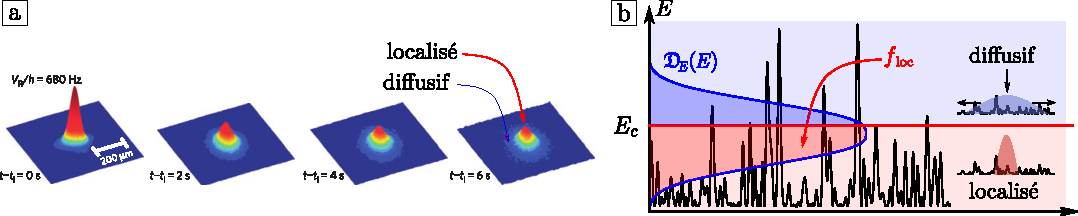
\includegraphics[width=\textwidth]{Fig/Introduction/AL3D.pdf}
\caption{\textbf{Observation de la localisation d'Anderson à trois dimensions.} \textbf{a:} images expérimentales de la localisation d'Anderson d'ondes de matière. Une partie des atomes reste localisée à temps long, tandis que le reste des atomes diffuse lentement. \textbf{b:} Illustration de la distribution d'énergie des atomes. La partie de basse énergie est localisée, tandis que la partie de haute énergie est diffusive. Ces comportements sont séparés par une transition de phase, d'énergie critique $\Ec$ appelée seuil de mobilité.}
\label{fig:AL3D}
\end{figure}

L'objectif de cette thèse était donc de dépasser les limitations expérimentales précédentes, telle qu'une limitation forte du temps de vie des atomes plongés dans le désordre, pour étendre le procédé de mesure des fonctions spectrales à la détermination du seuil de mobilité. Cependant, deux avaries majeures de l'expérience (détaillées dans la section suivante) n'ont pas rendu cette mesure possible dans le temps imparti. 

Ma contribution scientifique s'est alors focalisée sur l'exploitation des données expérimentales relatives au temps de diffusion élastique, obtenues lors de la thèse de Jérémie Richard \citep{richard2015propagation}\citep{richard2019elastic}, et leur confrontation aux mesures des fonctions spectrales \citep{signoles2019ultracold}. J'ai de plus réalisé des simulations numériques afin de compléter les mesures expérimentales, permettant de valider nos mesures du temps de diffusion élastique et de tester des modèles couramment utilisés pour la prédiction de ce dernier. Notamment, nous avons montré que l'approche des fonctions spectrales permet de décrire le comportement du temps de diffusion élastique sur la très large gamme de paramètres expérimentaux utilisée, permettant de sonder les régimes de désordre faible et de désordre fort. Cette étude nous a permis d'obtenir une vision très claire du processus de diffusion microscopique, qui constitue une brique élémentaire de la propagation d'ondes dans des milieux désordonnés.






\subsection{Contexte expérimental et déroulement de ma thèse}
%De premiers essais de stabilité du montage de désordre bichromatique, visant à dépasser la limitation du temps de vie des atomes dans le désordre identifiée lors de la mesure des fonctions spectrales, étaient en cours lors de mon arrivée à l'\emph{Institut d'Optique} en 2017. Une avarie du système informatique de contrôle de l'expérience, basé sur le logiciel \emph{Matlab}, a mis un terme à ces essais. Ce système, développé par l'ingénieur électronicien du laboratoire \emph{André Villing} parti à la retraite au cours de l'année 2017, a été remplacé par un système commercial \emph{National Instruments} et la suite \emph{Cicero Word Generator} développée au \emph{MIT} dans le groupe de \emph{Wolfgang Ketterle}. Ce remplacement, ainsi que la reconstruction de la séquence expérimentale, s'est déroulée de l'été 2017 jusqu'en mars 2018. Les changements informatiques associés ont été constants tout au long de ma thèse.
Peu après mon arrivée à l'\emph{Institut d'Optique} en 2017, un dysfonctionnement du système informatique de contrôle de l'expérience, basé sur le logiciel \emph{Matlab}, a fortement paralysé le reste de l'expérience. Ce système, développé par l'ingénieur électronicien du laboratoire \emph{André Villing} parti à la retraite au cours de l'année 2017, a été remplacé par un système commercial \emph{National Instruments} et la suite \emph{Cicero Word Generator} développée au \emph{MIT} dans le groupe de \emph{Wolfgang Ketterle}. Ce remplacement, ainsi que la reconstruction de la séquence expérimentale, s'est déroulée de l'été 2017 jusqu'en mars 2018. Les changements informatiques associés ont été constants tout au long de ma thèse. De manière plus générale, l'entièreté de l'expérience a été revue de fond en comble suite au remplacement de ce système.

\begin{figure}
\centering

\caption{\textbf{Chronologie du déroulement de ma thèse.} Stuff.}
\label{fig:chronologie_these}
\end{figure}

Au printemps 2018, une seconde avarie a paralysé l'expérience jusqu'au mois de novembre 2018. Une défaillance du circuit de refroidissement à eau des bobines de lévitation magnétique ont conduit au démontage d'une partie de l'expérience autour de la chambre de science. Des composants de génération du désordre, l'imagerie de la seconde chambre, des bobines de compensation de champs magnétiques et de lévitation ont ainsi été retirés du dispositif, puis remontés peu à peu. La calibration des champs magnétiques de la seconde chambre s'est déroulée entre le printemps et l'été 2019. L'étude du temps de diffusion élastique a eu lieu en parallèle de ces travaux de réparation, et ont duré jusqu'au printemps 2019.

Le printemps 2019 a aussi été marqué par le remplacement du laser fibré Ytterbium source pour notre piège dipolaire. La calibration de ce nouveau piège ainsi que l'optimisation de l'étape d'évaporation optique menant à la condensation de Bose-Einstein s'est déroulée jusqu'au début de l'année 2020. 

%L'entretien d'une expérience d'atomes ultra-froids nécessitant une présence quotidienne et un renouvellement constant de matériel, une mise à jour du système laser dédié au refroidissement est actuellement en cours. Nos lasers \emph{fait-maison} sont ainsi progressivement remplacés par des systèmes commerciaux \emph{Sacher Lasertechnik Cheetah}.




\section{Structure du manuscrit}
%\addcontentsline{toc}{section}{Structure du manuscrit}
Ce manuscrit se décompose selon les six chapitres suivants:
\begin{itemize}
\item[\textendash] \textbf{Chapitre \ref{ch:Localisation}: {\hypersetup{linkcolor=black}\nameref{ch:Localisation}}.} Nous commencerons par présenter les grandes lignes du transport quantique en milieu désordonné pour introduire le phénomène de localisation d'Anderson, pour ensuite nous attarder sur la transition de phase d'Anderson entre états localisés et états diffusifs. Nous nous concentrerons particulièrement sur l'état de l'art de la transition d'Anderson à l'aide des expériences d'atomes ultra-froids.  Nous ferons ainsi apparaître la quantité centrale de l'étude de la physique du désordre, la fonction spectrale. \\

\item[\textendash] \textbf{Chapitre \ref{ch:BEC_manip}: {\hypersetup{linkcolor=black}\nameref{ch:BEC_manip}}.} Dans un second temps, nous présenterons les grandes lignes de notre plateforme expérimentale. Nous rappellerons donc les principales propriétés d'un condensat de Bose-Einstein, ainsi que les différents processus d'interaction lumière-matière permettant de manipuler des atomes. Enfin, nous présenterons les différentes étapes d'un cycle expérimentales nous permettant d'obtenir un gaz quantique dégénéré. \\

\item[\textendash] \textbf{Chapitre \ref{ch:new_exp}: {\hypersetup{linkcolor=black}\nameref{ch:new_exp}}.} Après avoir présenté les différents éléments de notre expérience, nous allons nous focaliser sur les modifications apportées à notre dispositif au cours de ma thèse. En particulier, nous discuterons des deux éléments principaux de la chambre de science, la lévitation magnétique et le piège optique. Nos travaux sur ces éléments nous ont ainsi permis d'obtenir des condensats de Bose-Einstein bien meilleurs que précédemment, et de calibrer finement notre lévitation magnétique dans le but d'exploiter pleinement la dynamique de notre système. \\

\item[\textendash] \textbf{Chapitre \ref{ch:Speckle}: {\hypersetup{linkcolor=black}\nameref{ch:Speckle}}.} Après avoir présenté le dispositif générant notre onde de matière, nous décrirons notre milieu désordonné. Celui-ci est issu d'un champ de tavelures laser, ou \emph{speckle}, dont nous verrons les principales propriétés. Nous présenterons ainsi les différentes configurations de désordre que nous avons pu utiliser, et nous donnerons un aperçu de notre approche de désordre bichromatique visant à dépasser la contrainte du temps de vie limité des atomes dans le désordre à laquelle nous avons été confrontés. \\

\item[\textendash] \textbf{Chapitre \ref{ch:TauS_PRL}: {\hypersetup{linkcolor=black}\nameref{ch:TauS_PRL}}.} Ce chapitre se focalise sur la mesure du temps de diffusion élastique d'une onde de matière dans un potentiel désordonné optique. En suivant son évolution sur un large régime de paramètres, nous pourrons identifier le régime de diffusion faible pour lequel le temps de diffusion élastique est correctement décrit par l'approximation perturbative de Born. De plus, nous étudierons de manière quantitative la pertinence du critère de désordre faible $k_{\mathrm{i}}\ls^{\mathrm{Born}}=1$, et nous verrons que celui-ci dépend fortement de la nature du désordre considéré. \\

\item[\textendash] \textbf{Chapitre \ref{ch:TauS_NJP}: {\hypersetup{linkcolor=black}\nameref{ch:TauS_NJP}}.} Dans ce dernier chapitre, nous tacherons de décrire le comportement du temps de diffusion élastique à l'aide des fonctions spectrales. Nous verrons ainsi qu'une extension de l'approche perturbative ne permet pas d'étendre le domaine de validité de l'approximation de Born. De plus, nous verrons que l'approximation auto-consistante de Born, couramment utilisée, échoue à reproduire le comportement du temps de diffusion élastique dans un désordre de type \speckle . Nous verrons donc que la connaissance fine des détails de la fonction spectrale est nécessaire pour décrire la dynamique d'une onde de matière dans un désordre \speckle .
\end{itemize}


%\makeatletter
%\def\toclevel@chapter{0}
%\makeatother
%\setlength{\parskip}{0.5em}
%\part{Transport en milieu désordonné: phénomène de localisation}
\chapter{Phénomène de localisation d'Anderson} 
\label{ch:Localisation}
%\begin{tikzpicture}[remember picture, overlay]
%\node[anchor=north east,inner sep=0pt] at (current page.north east) {\includegraphics[scale=1]{Fig/Localisation/g825.png}};
%\end{tikzpicture}

Dans ce chapitre, nous commencerons par décrire comment, lors de la propagation cohérente d'une onde dans un milieu désordonné, les interférences peuvent altérer la diffusion classique et engendrer le phénomène spectaculaire de \emph{Localisation d'Anderson} dont nous donnerons les principales propriétés. Dans un second temps, nous présenterons succinctement les principaux systèmes utilisés pour l'investigation de la localisation d'Anderson, pour s'attarder plus particulièrement sur les expériences d'atomes froids. Enfin, nous terminerons ce chapitre par une discussion de nos enjeux actuels, l'étude du régime critique de la transition d'Anderson avec des atomes froids, dont nous présenterons l'état de l'art.

\section{Diffusion et interférences}
Cette première section a pour but de rappeler succinctement les mécanismes microscopiques à l'œuvre lors de l'étude de la propagation d'une onde dans un milieu désordonné, et comment le phénomène d'interférence peut modifier les grandeurs microscopiques associées. En particulier, nous nous focaliserons sur l'arrêt de la diffusion en conséquence de ces interférences, la localisation d'Anderson.

\subsection{Phénomène de diffusion}
\label{sc:diffusion_classique}
Le phénomène de diffusion macroscopique est un des phénomènes de transport les plus connus de la physique classique. Celui-ci permet par exemple de décrire de manière simple et unifiée la propagation de la chaleur dans un matériau homogène, l'homogénéisation de la concentration de particules dans un liquide ou encore le phénomène de résistance électrique. 

Le phénomène macroscopique de diffusion provient, de manière générale, de la marche aléatoire de particules au sein de leur environnement. Avec cette approche, Drude a par exemple été le premier à calculer la résistivité électrique des matériaux en introduisant un temps de relaxation microscopique basé sur des collisions élastiques entre les électrons, vecteurs du courant électrique, et les impuretés du matériau dans lequel ceux-ci se déplacent \citep{ashcroft2010solid}. 

Cet exemple historique illustre le fait que certaines propriétés macroscopiques des matériaux sont reliées aux grandeurs microscopiques de la marche aléatoire associée. Ces dernières grandeurs sont des briques élémentaires de la propagation en milieu désordonné, dont nous restreindrons l'étude au cas des collisions élastiques entre les particules et le désordre. Parmi ces briques élémentaires, que nous présenterons dans la suite, nous retrouvons le coefficient de diffusion, le temps de transport, ou encore le temps de diffusion élastique, auquel nous porterons une attention particulière.

\paragraph*{Temps de diffusion élastique}
La quantité la plus naturelle permettant de caractériser de manière microscopique le phénomène de diffusion est le \emph{temps de diffusion élastique} $\taus$, qui correspond à la durée typique entre deux évènements successifs de \emph{collision élastique} avec les impuretés du milieu. Ce temps est l'équivalent temporel du \emph{libre parcours moyen}  $\ls$ correspondant à la distance moyenne entre deux évènements de diffusion microscopiques successifs, illustrée figure \ref{fig:diffusion_classique}.a. Dans le cas d'une particule de masse $m$ se déplaçant à une vitesse $v_{\mathrm{i}}$, ces deux grandeurs sont reliées par
\begin{equation}
\taus=\frac{\ls}{v_{\mathrm{i}}}=\frac{m}{\hb} \frac{\ls}{k_{\mathrm{i}}} \text{ ,}
\label{eq:definition_taus}
\end{equation}
où $k_{\mathrm{i}}$ est le nombre d'onde de l'onde quantique associée à la particule (celui-ci est inchangé après chaque évènement de collision en raison de leur caractère élastique). 

Comme nous le verrons plus en détails dans les chapitres \ref{ch:TauS_PRL} et \ref{ch:TauS_NJP}, le temps de diffusion élastique est une quantité qui dépend des détails microscopiques du système et peut être interprété comme le temps de vie d'une onde plane dans le désordre.

\paragraph*{Temps de transport}
Si la norme du vecteur vitesse (ou de manière équivalente du vecteur d'onde) reste inchangée au cours de la propagation, sa direction est modifiée à chaque évènement de collision élastique. Comme nous le verrons plus en détails dans le chapitre \ref{ch:TauS_PRL}, lors de la collision avec un diffuseur de taille caractéristique $\sigma$, l'onde peut être diffusée selon un angle typique $\theta_{\mathrm{typ}}\sim 1/k_{\mathrm{i}} \sigma$. La diffusion peut donc être \emph{anisotrope}, en analogie avec la diffusion de Mie ou la diffraction en optique.

En considérant que la trajectoire d'une particule est composée de multiples collisions successives, il apparaît alors une seconde échelle de temps caractéristique, le \emph{temps de transport} ou temps de Boltzmann $\taub$, décrivant la durée nécessaire pour que la particule perde l'information de la direction initiale de sa vitesse. 


On peut ainsi montrer que le temps de transport (et son analogue spatial, la \emph{longueur de transport}) s'expriment en fonction du temps de diffusion élastique de la manière suivante \citep{akkermans2007mesoscopic}:
\begin{equation}
\taub=\frac{\taus}{1-\left\langle\cos{\theta}\right\rangle} \quad \text{et} \quad \lb=\frac{\ls}{1-\left\langle\cos{\theta}\right\rangle} \text{ ,}
\label{eq:definition_taub}
\end{equation}
où $\langle\:\cdots\:\rangle$ représente la valeur moyenne sur les différents évènements de diffusion, et $\theta$ l'angle de diffusion comme indiqué sur la figure \ref{fig:diffusion_classique}.a.

On voit donc que dans le cas de collisions élastiques isotropes, $\taub=\taus$, montrant qu'une seule collision suffit à perdre l'information sur la direction initiale de la vitesse de la particule. En revanche, un grand nombre de collisions sont nécessaires pour obtenir une isotropisation de la direction des vitesses dans le cas d'évènements de diffusion anisotrope.


\begin{figure}
\centering
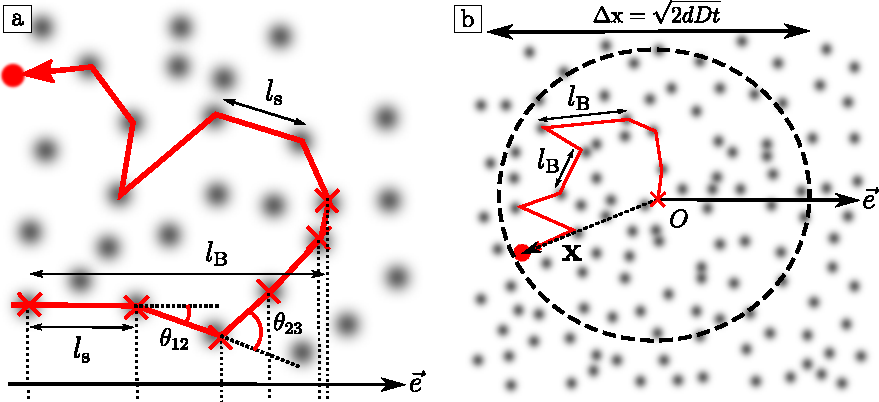
\includegraphics[width=\textwidth]{Fig/Localisation/diffusion_classique.pdf}
\caption{\textbf{a: Longueur de transport pour des collisions anisotropes.} Dans le cas de diffusion fortement anisotrope vers l'avant, une unique collision élastique ne modifie que peu la direction de la vitesse d'une particule. Il faut donc un grand nombre de collisions successives pour que la direction de la vitesse d'une particule soit décorrélée de la direction initiale. En conséquence, le temps de transport est beaucoup plus grand que le temps de diffusion élastique. \textbf{b: Mécanisme microscopique de la diffusion.} Le mouvement d'une particule peut être considérée comme une marche aléatoire composée d'évènements de diffusion isotropes tous les $\taub$ entre lesquels la particule se déplace d'une distance $\lb=v \taub$ dans une direction aléatoire. L'étalement typique obtenu croit avec le temps selon $\Delta \mathrm{x} =\sqrt{2dDt}$, avec $D$ le coefficient de diffusion.}
\label{fig:diffusion_classique}
\end{figure}





\paragraph*{Coefficient de diffusion}
Une fois que la particule a parcouru une distance $\lb$, on peut considérer qu'elle subit une diffusion isotrope. On assimile alors le mouvement des particules à une marche aléatoire pour laquelle les particules de vitesse $v$ subissent des évènements de collision isotrope à chaque intervalle de temps $\taub$ pendant lesquels la particule parcourt une distance $\lb=v \taub$, comme illustré figure \ref{fig:diffusion_classique}.b.

Ainsi, on peut déterminer l'étalement typique de la région explorée par la particule après $N$ collisions\footnote{On peut montrer que la probabilité qu'une particule ne subisse pas de collision isotrope sur une distance $x$ est donnée par $\mathcal{P}_x(x)=\frac{1}{\lb} e^{-x/\lb}$. La variance est alors obtenue par $\langle\Delta x^2 \rangle = \int_0^\infty{\diff x \: x^2 \:  \mathcal{P}_x(x)}=2\lb^2 $. Les $N$ collisions successives étant décorrélées, l'étalement typique de la région explorée est alors de $N \langle\Delta x^2 \rangle$.},
\begin{equation}
\left\langle \Delta \mathbf{x}^2 \right\rangle=2 N \lb^2 \text{ .}
\end{equation}
En définissant le coefficient de diffusion par $ \left\langle \Delta \mathbf{x}^2 \right\rangle = 2 d D t$ et en faisant apparaître le temps $t=N \taub$, on montre ainsi que \citep{akkermans2007mesoscopic}:
\begin{equation}
D=\frac{v \lb}{d}=\frac{\hb}{m d} k \lb \text{ ,}
\label{eq:definition_coefficient_diffusion}
\end{equation}
en faisant apparaître la quantité $k \lb$, qui sera essentielle dans la suite. Cette quantité peut être interprétée comme une mesure de la force du désordre comme nous aurons l'occasion de le voir dans la section \ref{sc:localisation_anderson} et dans le chapitre \ref{ch:TauS_PRL}. Notamment, le régime de désordre faible est défini par la condition $k\lb\gg 1$, signifiant que la distance entre deux collisions isotropes successives est très grande devant la longueur d'onde.

Une conséquence de l'équation \ref{eq:definition_coefficient_diffusion} est qu'une diminution de la longueur de transport entraîne une diminution du coefficient de diffusion. Ainsi, plus un système sera désordonné, plus le coefficient de diffusion sera petit.














\subsection{Localisation faible}
\label{sc:weak_localisation}
Si le mécanisme de marche aléatoire présenté permet de décrire un grand nombre de situations de diffusion classique, nous avons omis un ingrédient essentiel à la propagation d'ondes en milieu désordonné: la \emph{cohérence}, ou encore la capacité qu'une onde a à interférer. En particulier, nous verrons que celle-ci peut avoir des conséquences dramatiques sur les propriétés de transport d'une onde en présence de désordre.

\paragraph*{Mécanisme de localisation faible}
Pour cela, intéressons-nous à la probabilité $P(\mathbf{x},\mathbf{x}')$ qu'une onde initialement à la position $\mathbf{x}$ se retrouve à la position $\mathbf{x}'$ après propagation dans le milieu désordonné. Dans la limite $k\lb\gg 1$, la trajectoire de l'onde peut être vue comme une marche aléatoire, où chaque trajectoire de diffusion est associée à une amplitude complexe de probabilité $\left| A_j \right| e^{i \phi_j}$, avec $\phi_j$ la phase de la trajectoire. Ainsi, la probabilité $P(\mathbf{x},\mathbf{x}')$ est donnée par la somme de l'amplitude sur toutes les trajectoires possibles:
\begin{align}
P(\mathbf{x},\mathbf{x}') \nonumber&= \overline{{\left| \sum_j{ \left|A_j\right| e^{i \phi_j} }\right| }^2} = \overline{\sum_{j,l} {\left| A_j \right| \left| A_l \right| e^{i (\phi_j - \phi_l)}}} \\
&= \overline{\sum_j{{\left| A_j \right|}^2}} + \overline{\sum_{j\neq l}{\left| A_j \right| \left|A_l \right| e^{i(\phi_j - \phi_l)}}} \text{ ,}
\label{eq:amplitude_localisation_faible}
\end{align}
où $\overline{\:\cdots\:}$ désigne la moyenne sur les différentes réalisations du désordre.

Le premier terme décrit le phénomène de diffusion classique, pour lequel la probabilité $P(\mathbf{x},\mathbf{x}')$ est la somme des probabilités de chaque trajectoire. 

Le second terme de l'équation \ref{eq:amplitude_localisation_faible} représente quant à lui les interférences dues aux différentes phases accumulées par les différents chemins de diffusion. Intuitivement, on peut considérer que la contribution de ce terme s'annule en moyennant sur les différentes réalisations du désordre, $\overline{e^{i(\phi_j - \phi_l)}}=0$\footnote{L'annulation de ce second terme est à l'origine du traitement classique de la propagation d'ondes dans le désordre tels que dans la théorie de Drude ou du transfert radiatif.}. Cependant, une étude attentive montre que certaines trajectoires résistent au moyennage sur les réalisations du désordre.

En particulier, les trajectoires pour lesquelles l'onde se retrouve à son point de départ forment des boucles qu'il est possible de parcourir dans les deux sens, comme illustré figure \ref{fig:localisation_faible}. Par \emph{symétrie par renversement du temps}, la phase accumulée le long de ces trajectoires est identique pour les deux sens de propagation. De plus, ces paires de trajectoires existent quelque soit la réalisation du désordre, rendant ce processus d'interférences constructives robuste vis-à-vis du moyennage d'ensemble et $\overline{e^{i(\phi_j - \phi_l)}}=1$. Ainsi, la probabilité qu'une onde retourne à son point de départ est le double de la prédiction classique:
\begin{equation}
P(\mathbf{x},\mathbf{x})=2 \overline{\sum_j{{\left| A_j \right|}^2}} \text{ .}
\label{eq:proba_retour_origine}
\end{equation}

Les interférences entre chemins de diffusion tendent alors à favoriser le retour de l'onde à son point d'origine, ralentissant ainsi la diffusion. Cet effet de \emph{localisation faible}, commun à tout type d'onde, a été intensivement étudié aussi théoriquement que expérimentalement dans de nombreux domaines, tels qu'en physique des solides \citep{kramer1993localization}\citep{akkermans2007mesoscopic}, en optique \citep{wolf1985weak}\citep{mishchenko1993nature}, avec des ondes sismiques \citep{larose2004weak} ou encore avec des atomes froids \citep{jendrzejewski2012coherent}\citep{muller2015suppression}.


\begin{figure}
\centering
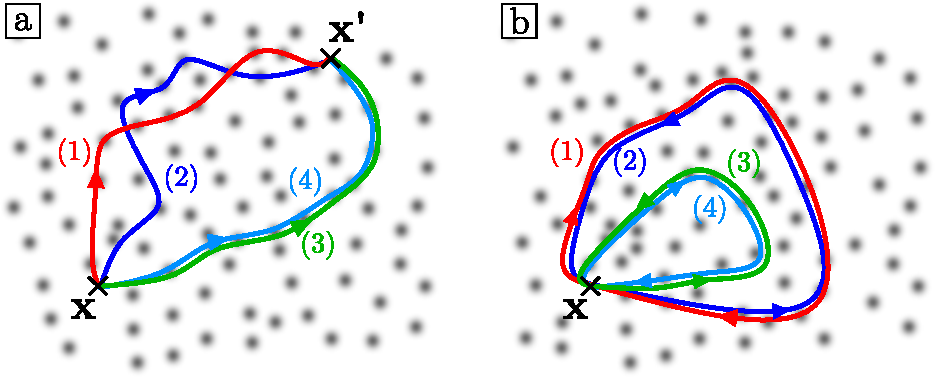
\includegraphics[width=0.9\textwidth]{Fig/Localisation/localisation_faible.pdf}
\caption{\textbf{a: Participation des différents chemins de diffusion à la propagation de l'onde.} La probabilité d'arriver au point $\mathrm{x'}$ en partant du point $\mathrm{x}$ est donnée par l'ensemble des trajectoires les reliant. Dans le cas des chemins 1 et 2, la phase accumulée le long de ces trajectoires diffère, détruisant en moyenne le phénomène d'interférence entre ces chemins. \textbf{b: Mécanisme de localisation faible.} Les chemins de diffusion pour lesquels l'onde retourne à son point de départ se présentent sous forme de boucles qu'il est possible de parcourir dans les deux sens, comme illustré par les trajectoires 1 et 2, ou encore les trajectoires 3 et 4. Ces paires de trajectoires existent quelle que soit la réalisation du désordre.}
\label{fig:localisation_faible}
\end{figure}



\paragraph*{Corrections de localisation faible}
Comme le montre l'équation \ref{eq:proba_retour_origine}, le retour de l'onde à son point d'origine est favorisé à l'aide des interférences constructives qu'il existe entre des trajectoires symétriques par renversement du temps. Notamment, cet effet de localisation faible se traduit par la diminution du coefficient de diffusion par rapport à la prédiction classique \ref{eq:definition_coefficient_diffusion}, que l'on peut alors écrire sous la forme
\begin{equation}
D= D_{\mathrm{0}}-\delta D \text{ ,}
\end{equation}
où $D_{\mathrm{0}}$ est le coefficient de diffusion classique \ref{eq:definition_coefficient_diffusion}, et $\delta D$ est la correction de localisation faible. Ces corrections de localisation faible dépendent des détails microscopiques du système, mais aussi de sa dimension $d$ et de sa taille $L$. En estimant le poids des boucles de localisation faible, on peut montrer que \citep{akkermans2007mesoscopic}:
\begin{equation}
\delta D/ D_{\mathrm{0}} = \left\lbrace \begin{aligned}
& \mathcal{O}\left(L/l_{\mathrm{B}}\right)  \quad &&\text{en 1D ,}\\
& \mathcal{O}\left(\frac{1}{k l_{\mathrm{B}}} \ln{\frac{L}{l_{\mathrm{B}}}} \right) \quad &&\text{en 2D ,}\\
& \mathcal{O}\left(\frac{1}{(k l_{\mathrm{B}})^2}\right) \quad &&\text{en 3D .}
\end{aligned}\right.
\label{eq:correction_localisation_faible}
\end{equation}
Ces relations témoignent ainsi de la forte influence de la dimension du système comme nous le verrons plus en détails dans la section suivante.






\subsection{Suppression du transport: Localisation d'Anderson}
\label{sc:localisation_anderson}

Les corrections de localisation faible données par l'équation \ref{eq:correction_localisation_faible} font apparaître un comportement remarquable: sous certaines conditions, il est possible que la correction $\delta D$ soit égale au coefficient de diffusion classique $D_{\mathrm{0}}$, entraînant ainsi la suppression du transport avec $D=0$. Cet effet dit de \emph{Localisation forte}, ou encore de \emph{Localisation d'Anderson}, a été découvert en 1958\footnote{Le phénomène de localisation d'Anderson a été découvert avant les processus de localisation faible.} par \emph{Philip W. Anderson} s'intéressant alors à la diffusion d'une particule quantique dans un réseau désordonné dans le cadre de la physique de la matière condensée \citep{anderson1958absence}. Cette inhibition du transport constitue la signature la plus spectaculaire de l'influence de la cohérence de l'onde lors de sa propagation dans un milieu désordonné. Ces travaux furent récompensés par le prix Nobel de physique en 1977, conjointement avec \emph{Sir Nevill Francis Mott} et \emph{John Hasbrouck van Vleck}. 



\paragraph*{Localisation d'Anderson et rôle de la dimension}
Dans le régime \emph{isolant}\footnote{Par opposition au régime \emph{métallique} où le transport existe.} de localisation d'Anderson, la fonction d'onde reste localisée aux alentours du point d'origine et présente un profil exponentiel
\begin{equation}
\left| \psi (\mathbf{x}) \right|^2 \propto e^{-\mathrm{x}/\xiloc} \text{ ,}
\label{eq:exponentielle_anderson}
\end{equation}
où $\xiloc$ correspond à la longueur typique sur laquelle l'onde s'étend, et est appelée \emph{longueur de localisation}\footnote{La longueur de localisation est définie comme la longueur caractéristique de décroissance des ailes de la fonction d'onde moyenne $\xiloc=\lim\limits_{x\rightarrow\infty} -\frac{x}{\;\overline{\ln|\psi(x)|^2}\;}$.}.

Pour un système de taille suffisamment grande, les corrections de localisation faible $\delta D$ de l'équation \ref{eq:correction_localisation_faible} en dimension 1 sont du même ordre que le coefficient de diffusion classique $D_{\mathrm{0}}$. On constate ainsi qu'en dimension 1, les processus de localisation faible sont très efficaces, rendant tous les états localisés. Il est possible d'estimer la longueur de localisation à l'aide des corrections de localisation faible en écrivant $\delta D(\xiloc)\sim D_{\mathrm{0}}$, d'où on déduit que $\xiloc=2 \lb$ pour un système unidimensionnel. De fait, la localisation d'Anderson se manifeste même pour des désordres faibles, témoignant de son caractère spectaculaire. 


De même, à deux dimensions, il apparaît des corrections de localisation faible \ref{eq:correction_localisation_faible} que tous les états sont localisés pour un système de taille suffisamment grande. En écrivant $\delta D(\xiloc)\sim D_{\mathrm{0}}$, on trouve ainsi que les états restent localisés mais sur des échelles de longueurs bien plus grandes que dans le cas unidimensionnel, de l'ordre de $\xiloc \sim \lb \exp{(k \lb)}$. Pour des désordres faibles ($k \lb \gg 1$), la longueur de localisation excède généralement la taille du système. On parle ainsi de dimension \emph{marginale} de la localisation d'Anderson.

Remarquablement, les corrections de localisation faible à trois dimensions ne dépendent pas de la taille du système, mais seulement de la force du désordre $k \lb$. Dans le cas d'un désordre faible ($k\lb\gg 1$), les boucles de localisation faible ne sont pas assez nombreuses pour changer de manière significative la dynamique diffusive de l'onde ($\delta D \ll D_{\mathrm{0}}$). En revanche, la localisation d'Anderson persiste dans le cas d'un désordre fort où $k \lb \leq 1$, pour lequel la phase de l'onde varie peu entre deux évènements successifs de diffusion. 

Notons que l'analyse intuitive des propriétés de localisation en fonction de la dimension à l'aide des corrections de localisation faible présentée ici a été rigoureusement étudiée et validée dans le cadre de la \emph{théorie d'échelle de la localisation d'Anderson}, développée à la fin des années 1970 \citep{abrahams1979scaling}.

\paragraph*{Transition d'Anderson à trois dimensions}
Il apparaît donc que le cas à trois dimensions présente un intérêt particulier. En effet, un même système peut, selon la force du désordre, présenter un comportement qui soit métallique ou isolant. Selon l'équation \ref{eq:correction_localisation_faible}, on peut estimer que ce changement de comportement se manifeste lorsque
\begin{equation}
k \lb \sim 1 \text{ ,}
\label{eq:ioffe_regel}
\end{equation}
condition connue sous le nom de \emph{critère de Ioffe-Regel}. 

Il est possible de donner une interprétation intuitive au critère de Ioffe-Regel en se focalisant sur la phase accumulée par l'onde entre deux évènements successifs de diffusion. En effet, cette phase est de l'ordre de $\phi\sim k\lb$. Dans le régime de désordre fort, la phase de l'onde est donc similaire pour plusieurs évènements de diffusion successifs, générant ainsi des interférences constructives entre les différentes ondes diffusées. 

Plus particulièrement, il a été montré à l'aide la théorie d'échelle de la localisation d'Anderson qu'il existe une transition de phase du deuxième ordre entre états localisés et états diffusifs pour des systèmes à trois dimensions \citep{abrahams1979scaling}. Le paramètre de contrôle de la transition étant l'énergie $E$ de l'onde, la transition d'Anderson possède donc une énergie critique $\Ec$ appelée \emph{seuil de mobilité}, comme illustré figure \ref{fig:transition_anderson}.a. 

La transition d'Anderson est de plus caractérisée par deux exposants critiques $\nu$ et $s$, décrivant respectivement comment la longueur de localisation $\xiloc$ diverge pour des états localisés proches du seuil de mobilité et comment le coefficient de diffusion $D$ s'approche de $0$ pour des états diffusifs (voir figure \ref{fig:transition_anderson}.b):
\begin{equation}
D \sim \left| E-\Ec \right|^s \quad \text{et} \quad \xi_{\mathrm{loc}} \sim \left| E-\Ec \right|^{-\nu} \text{ .}
\end{equation}
Bien qu'aucune théorie ne puisse décrire exactement le régime critique de la transition d'Anderson à l'heure actuelle, plusieurs études numériques s'accordent sur les valeurs $s=\nu=1.58$ des exposants critiques \citep{slevin1999corrections} \citep{evers2008anderson} \citep{slevin2014critical}. À ce jour, seule une expérience \textit{indirecte} a été capable de mesurer ces exposants critiques (voir section \ref{sc:localisation_atomes_froids}) \citep{lopez2012experimental}


\begin{figure}
\centering
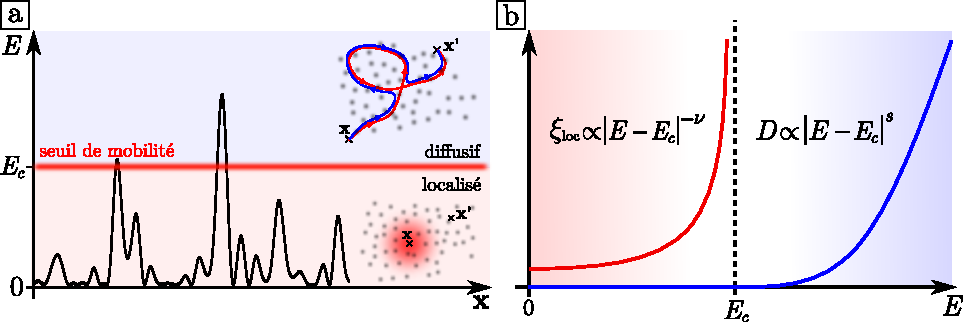
\includegraphics[width=\textwidth]{Fig/Localisation/transition_anderson.pdf}
\caption{\textbf{a: Transition d'Anderson.} À trois dimensions, il existe une transition de phase entre états diffusifs et états localisés. Pour une énergie supérieure à l'énergie critique de la transition, appelée seuil de mobilité, l'onde peut diffuser, tandis que pour une énergie inférieure au seuil de mobilité, l'onde est localisée. \textbf{b: Régime critique.} La transition d'Anderson est caractérisée par les exposants critiques $s$ et $\nu$, qui décrivent comment évoluent la longueur de localisation et la coefficient de diffusion aux alentours du seuil de mobilité. Dans le régime critique localisé, la longueur de localisation diverge en s'approchant du seuil de mobilité avec un exposant $\nu$. Dans le régime critique diffusif, le coefficient de diffusion s'annule selon une loi de puissance d'exposant $s$. }
\label{fig:transition_anderson}
\end{figure}
%\subsection{Théorie d'échelle}















\section{Localisation des atomes froids}
La localisation d'Anderson étant due au caractère ondulatoire du système étudié, celle-ci est donc commune à tout type d'onde, qu'elle soit classique (ondes lumineuses ou acoustiques) ou quantique (ondes électroniques, ondes de matière). Ce phénomène a donc été étudié expérimentalement à l'aide d'un grand nombre de systèmes dont nous allons brièvement présenter les principaux résultats ici, en mettant l'accent sur la transition métal-isolant.

\subsection{Etudes expérimentales de la localisation d'Anderson}
L'étude expérimentale de la localisation d'Anderson constitue un domaine de recherche qui s'est énormément développé, débutant dans les années 70-80 avec des systèmes électroniques et faisant aujourd'hui encore l'objet de recherches intenses.

\paragraph*{Localisation dans les systèmes électroniques}
Les premières expériences furent menées à l'aide de systèmes électroniques, et purent démontrer des effets de localisation faible ainsi que des effets de localisation forte \citep{mott1979electronic}\citep{paalanen1983critical}. Rapidement, les efforts se sont concentrés sur l'observation de la transition métal-isolant\footnote{Cette dénomination prend tout son sens dans les systèmes électroniques: les expériences menées correspondent à des mesures de conductivité.} prédite par la théorie d'échelle de la localisation. 

Cependant, une étude quantitative de la transition s'est révélée ardue en raison de la complexité de ces systèmes. En particulier, la présence d'interactions coulombiennes entre les électrons modifie profondément les propriétés de localisation, et rend délicate la distinction expérimentale entre la transition métal-isolant liée au désordre (transition d'Anderson) et la transition métal-isolant liée aux interactions (transition de Mott). Ces effets sont particulièrement marqués par la comparaison entre les exposants critiques mesurés ($\nu\sim 1$ pour \citep{shlimak1996determination}) et ceux estimés à l'aide de simulations numériques ($\nu\sim1.58$). Notons tout de même que de nouvelles expériences rapportent l'observation de la localisation d'Anderson à l'aide systèmes électroniques \citep{siegrist2011disorder}\citep{ying2016anderson}.

\begin{figure}
\centering
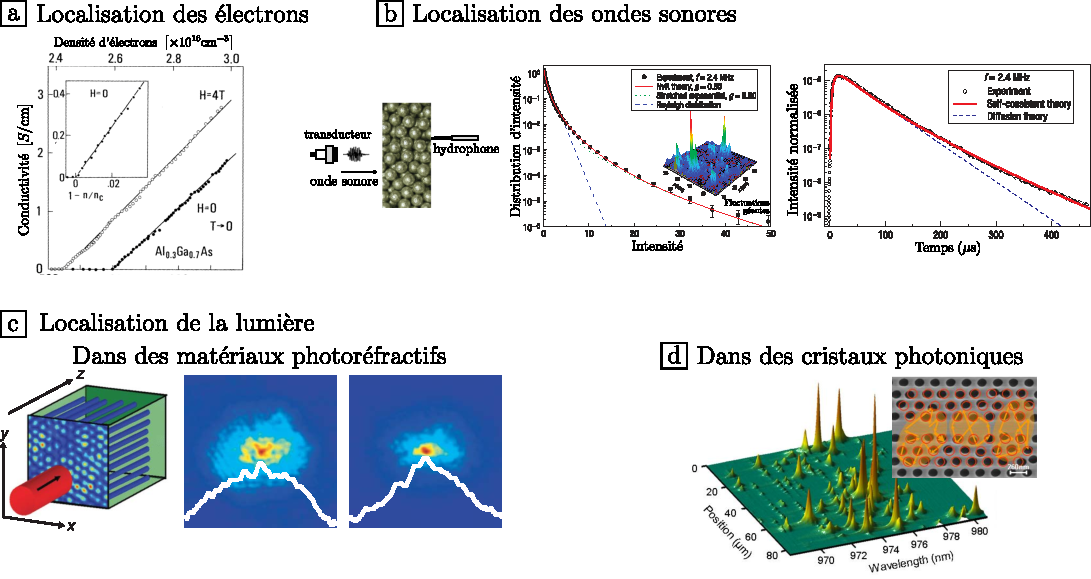
\includegraphics[width=\textwidth]{Fig/Localisation/experiences_localisation_anderson.pdf}
\caption{\textbf{Etudes expérimentales de la localisation d'Anderson.} \textbf{a:} A basse température, un métal peut devenir isolant à cause du désordre, sa conductivité s'annulant alors. Cette transition peut être atteinte en diminuant la densité d'électrons. Figure tirée de \citep{katsumoto1987fine}. \textbf{b:} La localisation d'Anderson d'ondes élastiques dans un réseau désordonné de billes d'aluminium peut être étudiée à l'aide d'un hydrophone après sa propagation. Il est possible de relever la distribution d'intensité de l'onde ainsi que son profil temporel qui présentent des signatures de la localisation d'Anderson. Figures tirées de \citep{hu2008localization}. \textbf{c} et \textbf{d:} La localisation de la lumière peut être étudiée à l'aide de plusieurs systèmes, tels que des matériaux photoréfractifs composés d'un réseau désordonné de guides d'ondes (\textbf{c}, figure tirée de \citep{schwartz2007transport}) ou encore dans des cristaux photoniques (\textbf{d}, figure tirée de \citep{sapienza2010cavity}).}
\label{fig:experiences_localisation_anderson}
\end{figure}

\paragraph*{Localisation dans les systèmes classiques} 
L'utilisation des ondes classiques s'est alors imposée comme étant un moyen de réaliser des systèmes mieux contrôlés que dans le cadre de la matière condensée. Les premières signatures de la localisation d'Anderson ont été obtenues dans les années 90 avec des ondes ultrasonores \citep{weaver1990anderson}, des ondes mécaniques de flexion \citep{ye1992observation}, des micro-ondes \citep{genack1991observation} ainsi que des ondes lumineuses \citep{wiersma1997localization}. 

Cependant, ces premières expériences s'appuyaient sur la décroissance exponentielle de l'intensité de l'onde pour analyser leurs résultats. Leur interprétation fut controversée en raison de l'existence d'autres phénomènes présentant la même signature, en particulier l'absorption qui présente aussi une décroissance exponentielle de l'intensité de l'onde comme décrit par la loi de Beer-Lambert \citep{scheffold1999localization}. Depuis, d'autres signatures ont été exploitées telle que la dynamique de l'onde en régime pulsé \citep{weaver1993anomalous} ou encore les fluctuations géantes de transmission \citep{nieuwenhuizen1995intensity} afin d'observer sans ambiguïté la localisation d'Anderson.

Aujourd'hui encore, la difficulté expérimentale s'accroît fortement en augmentant la dimension du système. En particulier, augmenter le pouvoir diffusant du milieu à trois dimensions afin d'atteindre le critère de Ioffe-Regel $k \lb \sim 1$ tout en s'affranchissant de l'absorption reste un tour de force expérimental. Ainsi, la seule observation de la localisation d'Anderson à trois dimensions faisant consensus à été réalisée au Canada dans le groupe de J. Page à l'aide d'ondes acoustiques se propageant dans des billes d'aluminium \citep{hu2008localization}.

Notons finalement que la localisation à trois dimensions d'ondes lumineuses fait l'objet de recherches intenses très débattues. Enfin, une récente étude numérique prédit l'absence de la localisation d'Anderson à trois dimensions dans le cas d'ondes lumineuses en raison de leur caractère vectoriel \citep{skipetrov2014absence}.












\subsection{L'approche des atomes froids}
\label{sc:localisation_atomes_froids}
Depuis le milieu des années 2000, une nouvelle plateforme participe à l'étude de la physique du désordre: les atomes ultra-froids. Ces systèmes, utilisés en interférométrie atomique et pour de la simulation quantique, sont bien connus pour leurs propriétés de cohérence sous forme de \emph{condensats de Bose-Einstein}. Ceux-ci présentent un degré de contrôle inédit et offrent des possibilités expérimentales complexes qu'il est impossible d'obtenir à l'aide d'autres systèmes.

En effet, les expériences d'atomes ultra-froids présentent un grand nombre d'avantages: il est possible d'imager la fonction d'onde des atomes aussi bien dans l'espace réel grâce à une imagerie \emph{in-situ} que dans l'espace des vitesses à l'aide d'une imagerie par \emph{temps de vol}. De plus, les atomes ultra-froids ne présentent pas d'absorption, et dépassent ainsi les difficultés des expériences pionnières d'observation de la localisation d'Anderson. Enfin, de tels systèmes offrent un vaste contrôle des paramètres microscopiques, de l'onde comme du désordre en passant par la dimension. Les atomes ultra-froids apparaissent alors comme une plateforme idéale pour étudier la physique du désordre.


\paragraph*{Atomes ultra-froids et désordre}
Il existe différentes méthodes pour générer un désordre sur les atomes. Parmi les plus utilisées on retrouve les champs de tavelures optiques, ou \emph{speckle}, et les réseaux bichromatiques pour lesquels un réseau de faible amplitude vient moduler de manière quasi-aléatoire le réseau principal (voir figure \ref{fig:localisation_1D_atomes_froids}). Notons aussi le développement récent de désordres générés à l'aide de modulateurs spatiaux de lumière ou de matrices de micro-miroirs, permettant de réaliser des profils d'illumination arbitraires.

Toutes ces façons de réaliser un désordre pour les atomes possèdent un point commun: ils sont générés à l'aide de champs lumineux et possèdent donc une longueur typique de variation, ou \emph{longueur de corrélation} $\sigma$, généralement de l'ordre du micromètre. L'existence de cette longueur typique impose une température critique pour le système présente un comportement quantique. En particulier, les effets quantiques associés au comportement ondulatoire de la matière sont attendus lorsque la longueur de \emph{de Broglie} est plus grande que la longueur de corrélation:
\begin{equation}
\ldb\geq\sigma \quad \text{soit} \quad T_{\mathrm{typ}} \leq \frac{\hb^2}{ \kB m \sigma^2}\sim \text{ quelques nanokelvins.}
\end{equation}
L'observation d'effets quantiques en présence de désordre nécessite donc des températures extraordinairement basses qui sont typiquement obtenues avec des \emph{condensats de Bose-Einstein}. 

\begin{comment}
Cependant, l'obtention de telles températures n'est pas nécessaire pour observer la dynamique diffusive d'atomes dans un désordre optique. Notamment, celle-ci a été étudiée en deux dimensions en se concentrant sur la décroissance temporelle de la densité atomique \citep{robert2010anisotropic}. Plus particulièrement, une décroissance de la densité atomique en $1/t$ au centre du nuage servant de point source, signature de la dynamique diffusive, a été observée en présence de désordre, tandis que celle-ci est caractérisée par une décroissance en $1/t^2$ pour une expansion balistique en absence de désordre.
\end{comment}







\paragraph*{Localisation d'Anderson d'ondes atomiques}
C'est en 2008 qu'a été observée la localisation d'Anderson d'ondes de matière simultanément dans deux expériences illustrées sur la figure \ref{fig:localisation_1D_atomes_froids}. L'expérience de Billy et al. \citep{billy2008direct}, menée au Laboratoire Charles Fabry à Palaiseau, rapporte l'arrêt de l'expansion d'un condensat de Bose-Einstein de \isotope[87]{Rb} dilué et plongé dans un guide d'onde optique unidimensionnel ainsi que dans un désordre de type speckle. De plus, la mesure du profil de densité atomique montre la décroissance exponentielle \ref{eq:exponentielle_anderson} de la fonction d'onde localisée, comme représenté figure \ref{fig:localisation_1D_atomes_froids}.a. 

La seconde expérience, réalisée par Roati et al. \citep{roati2008anderson} au LENS à Florence, rapporte aussi l'arrêt de l'expansion d'un condensat de Bose-Einstein de \isotope[39]{K} placé dans un potentiel unidimensionnel composé d'un réseau bichromatique\footnote{L'arrêt de l'expansion du paquet d'onde rapporté par les auteurs ne correspond à proprement parler de localisation d'Anderson, le réseau bichromatique ne constituant pas un système n'étant pas réellement désordonné. Le modèle d'Aubry-André décrivant ce système n'appartient pas à la même classe d'universalité que le modèle d'Anderson, et présente notamment une transition de phase en dimension 1 \citep{sarma1988mobility}.} représenté figure \ref{fig:localisation_1D_atomes_froids}.b. L'utilisation d'atomes de \isotope[39]{K} permet de contrôler les interactions inter-atomiques à l'aide d'une résonance de Feshbach et constitue la grande force de cette expérience.

Ces expériences ont ainsi démontré la pertinence des atomes ultra-froids pour l'étude des systèmes désordonnés. Ces résultats novateurs ont par suite déclenché de nombreux efforts expérimentaux pour l'étude de la localisation d'Anderson dans des systèmes de dimensions plus élevées, $d=2$ et notamment en dimension $d=3$ dans le but d'étudier la transition métal-isolant d'Anderson. 

\begin{figure}
\centering
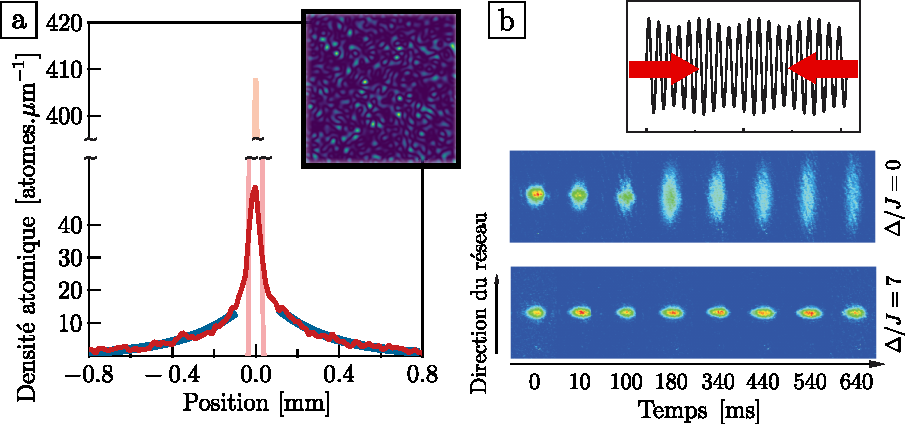
\includegraphics[width=\textwidth]{Fig/Localisation/localisation_1D_atomes.pdf}
\caption{\textbf{Premières expériences de localisation unidimensionnelle.} \textbf{a:} Localisation d'Anderson unidimensionelle d'ondes de matière dans un speckle. La densité atomique est mesurée après une seconde d'expansion dans un guide d'onde unidimensionnel et dans un potentiel de type speckle. Les ailes du profil sont caractérisées par un décroissance exponentielle (traits bleus). Le profil rose correspond à la densité atomique initiale. Figure tirée de \citep{billy2008direct}. \textbf{b:} Localisation d'ondes atomiques dans un réseau bichromatique unidimensionnel. Un condensat de Bose-Einstein s'étend dans l'espace libre (image du haut), tandis que son expansion est arrêtée lorsque celui-ci est placé dans un potentiel quasi-périodique (image du bas). Figure tirée de \citep{roati2008anderson}. }
\label{fig:localisation_1D_atomes_froids}
\end{figure}

\paragraph*{Localisation d'Anderson à deux dimensions}
L'observation expérimentale de la localisation d'Anderson à deux dimensions constitue un véritable tour de force se heurtant à deux obstacles majeurs. Comme nous avons vu précédemment, la longueur de localisation $\xiloc$ dépend de manière exponentielle de la force du désordre $k\lb$, et requiert l'utilisation de systèmes particulièrement larges\footnote{Les dimensions nécessaires sont plus grandes que $\SI{100}{\micro\metre}\times\SI{100}{\micro\metre}$, correspondant à des systèmes de grande taille pour des atomes ultra-froids \citep{white2019observation}.}. L'observation d'effets quantiques ($\ldb>\sigma$) nécessite alors que les potentiels optiques désordonnés possèdent une grande résolution optique sur l'ensemble du système.

Une seconde contrainte expérimentale forte provient de la distinction entre localisation d'Anderson, d'origine quantique, et le piégeage classique. Si les désordres de type speckle sont adaptés pour des systèmes unidimensionnels et tridimensionnels \citep{pilati2010dilute}, ceux-ci présentent un seuil de percolation classique particulièrement élevé en deux dimensions \citep{morong2015simulation}. L'utilisation d'un désordre fort, nécessaire pour l'observation de la localisation d'Anderson à deux dimensions, ne permet alors pas de distinguer cette dernière de la percolation classique.

Ce n'est que récemment (2019) que ces contraintes ont pu être contournées et que la localisation d'Anderson à deux dimensions a pu être observée à l'aide d'atomes ultra-froids. White et al. \citep{white2019observation} rapportent ainsi l'observation de la localisation d'Anderson en deux dimensions à l'aide d'une expérience de transmission entre deux réservoirs connectés par un canal désordonné. Les auteurs témoignent du profil exponentiel de la fonction d'onde localisée dans le canal désordonné. Ceux-ci ont pu contourner les obstacles présentés précédemment à l'aide un désordre optique généré par un modulateur spatial de lumière, permettant de contrôler le seuil de percolation classique en changeant la densité de diffuseurs dans le canal. 



\paragraph*{Localisation d'Anderson en trois dimensions}
C'est principalement vers l'étude de la localisation d'Anderson à trois dimensions et plus particulièrement vers l'étude de la transition de phase que ce se sont concentrés les efforts expérimentaux après l'observation de la localisation d'Anderson dans des systèmes unidimensionnels. Notamment, l'étude expérimentale du seuil de mobilité et plus généralement du régime critique de la transition d'Anderson reste un sujet de recherche d'actualité \citep{pasek2017anderson}.

Trois expériences rapportent l'observation de la localisation d'Anderson à trois dimensions. Le groupe de B. de Marco à Urbana Champaign a ainsi utilisé un gaz fermionique de \isotope[40]{K} dans un potentiel speckle anisotrope \citep{kondov2011three}. Simultanément, l'équipe de Palaiseau a observé un arrêt de l'expansion d'une partie du nuage d'atomes de \isotope[87]{Rb} plongé dans un désordre isotrope généré par la superposition cohérente de deux speckles, pour des durées d'observation allant jusqu'à \SI{6}{\second} \citep{jendrzejewski2012three}. Enfin, une expérience récente menée au LENS dans l'équipe de G. Modugno rapporte l'observation de la localisation complète du nuage atomique de \isotope[39]{K}, dont les interactions ont été annulées à l'aide de résonances de Feshbach \citep{semeghini2015measurement}.

Ces trois expériences constituent une étape capitale de l'étude de la localisation d'Anderson avec des atomes froids. En dépit de ce premier succès, ces expériences n'ont cependant pas permis d'adresser l'étude du régime critique et définissent ainsi le contexte de cette thèse, comme nous le verrons plus en détails dans la section \ref{sc:etat_art_transition}. 

\begin{figure}
\centering
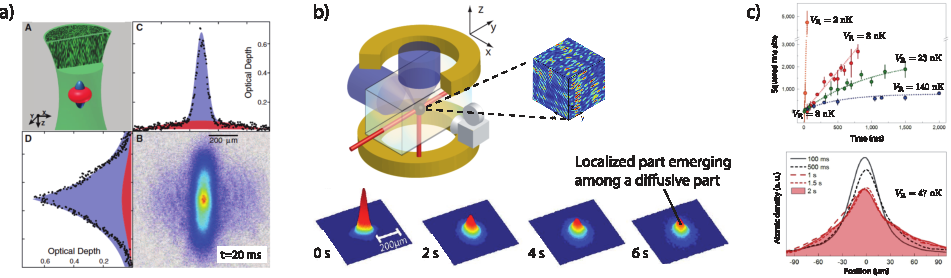
\includegraphics[width=\textwidth]{Fig/Localisation/localisation_3D_atomes_v1.pdf}
\caption{\textbf{Observation de la localisation d'Anderson à trois dimensions avec des atomes ultra-froids.} \textbf{a:} Localisation d'une partie du nuage de \isotope[40]{K} à temps très court. Une partie localisée émerge du centre d'un fond balistique. Figure tirée de \citep{kondov2011three}. \textbf{b:} Observation à temps très long d'une partie localisée du nuage de \isotope[87]{Rb} qui se démarque d'un fond très peu diffusif dans un désordre quasi-isotrope. Figure tirée de \citep{jendrzejewski2012three}. \textbf{c:} Localisation d'un nuage de \isotope[39]{K} complet dont les interactions sont annulées à l'aide d'une résonance de Feshbach. Figure tirée de \citep{semeghini2015measurement}.}
\label{fig:localisation_3D_atomes_froids}
\end{figure}





\paragraph*{Localisation dynamique}
Notons enfin l'existence d'un autre système permettant d'étudier la localisation d'Anderson à l'aide d'atomes froids, basé sur le phénomène de \emph{localisation dynamique}. Développé expérimentalement dans les années 1990 \citep{moore1995atom}, le système de \emph{rotateurs forcés} (ou \emph{kicked rotors} en anglais) repose sur un mapping entre un rotateur pulsé périodiquement et un modèle d'Anderson. Celui-ci se focalise sur l'apparition du phénomène de localisation dans l'espace des vitesses \citep{lemarietel-00424399}. 

En effet, à l'aide d'une onde stationnaire pulsée périodiquement, équivalente à une transmission périodique d'impulsion aléatoire, on peut décrire le mouvement des atomes soumis à ces \emph{kicks} comme une marche aléatoire dans l'espace des vitesses. Cependant, la richesse de ce système réside dans sa dynamique quantique, grâce à laquelle le phénomène de localisation apparaît de manière équivalente à celle dans l'espace réel et présente une localisation exponentielle de la distribution de vitesses des atomes illustrée figure \ref{fig:kicked_rotors}.

\begin{figure}
\centering
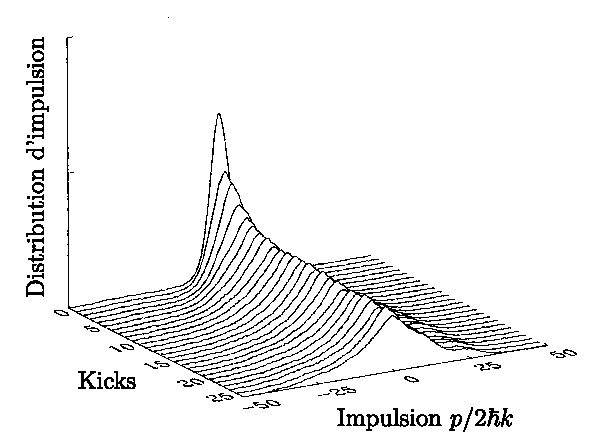
\includegraphics[width=0.6\textwidth]{Fig/Localisation/kicked_rotor.pdf}
\caption{\textbf{Localisation dynamique d'atomes froids.} Un nuage d'atomes de sodium est soumis à des kicks périodiques, induisant une marche aléatoire dans l'espace des impulsions. Après un certain nombre de kicks, la distribution d'impulsion se fige et présente une décroissance exponentielle. Figure tirée de \citep{moore1995atom}. }
\label{fig:kicked_rotors}
\end{figure}

L'extension du kicked rotor unidimensionnel à des dimensions supérieures $d=2$ et $d=3$ a pu se faire à l'aide d'une modulation temporelle des kicks \citep{casati1989anderson}. Le \emph{kicked rotor quasi-périodique} possède une transition de phase métal-isolant d'Anderson, confortée par l'existence d'un mapping \citep{lemarie2009observation} ainsi que par des études numériques \citep{lemarie2009universality}. L'expérience de Chabé et al. \citep{chabe2008experimental} réalisée à Lille rapporte ainsi une valeur de $\nu=1.63\pm0.05$ de l'exposant critique de la transition de phase associée, tout en vérifiant l'universalité de celle-ci \citep{lopez2012experimental}. Cette mesure constitue aujourd'hui encore la seule mesure expérimentale des exposants critiques de la transition d'Anderson compatible avec les estimations numériques \citep{slevin2014critical}.








\section{Vers l'étude du régime critique}
Nous avons vu dans la section précédente que la plateforme des atomes ultra-froids constitue un outil idéal pour étudier la problématique de la propagation cohérente d'ondes dans des milieux désordonnés. En revanche, malgré l'observation de la localisation d'Anderson dans des systèmes unidimensionnels et tridimensionnels, l'étude à énergie résolue de la transition d'Anderson reste un défi de taille auquel les trois expériences menées n'ont pas pu apporter de réponse.

Dans cette partie, nous allons donc décrire les limitations des différentes expériences afin de dresser un état de l'art de l'étude de la transition d'Anderson avec des atomes ultra-froids. Enfin, nous nous pencherons brièvement sur l'approche suivie par notre équipe pour tenter de dépasser ces limitations, approche qui sera plus amplement détaillée dans le chapitre \ref{ch:TauS_NJP}.

\subsection{Etat de l'art de l'étude de la transition d'Anderson avec des atomes ultra-froids}
\label{sc:etat_art_transition}
Comme nous allons le voir plus en détails, les trois expériences de localisation d'Anderson d'onde de matière à trois dimensions menées jusqu'à présent ont pour similarité d'estimer indirectement le seuil de mobilité $\Ec$. Si la détermination précise du seuil de mobilité constitue une première étape cruciale vers l'étude du régime critique de la transition d'Anderson, celle-ci n'en reste pas moins un véritable défi expérimental. Il est donc important de présenter les résultats de ces premières expériences afin de contextualiser les travaux réalisés dans le cadre de cette thèse.

\begin{comment}
Contrairement aux exposants critiques de la transition d'Anderson, l'énergie critique de la transition, le seuil de mobilité, n'est pas universelle et dépend des détails microscopiques du désordre. L'utilisation de désordres de type speckle par les expériences, de distribution asymétrique (voir chapitre \ref{ch:Speckle}), résultent en un comportement complexe du seuil de mobilité, qui diffère entre potentiels répulsifs ou attractifs. 
\end{comment}

\paragraph*{Expérience d'Urbana Champaign}
La première expérience à donner une estimation du seuil de mobilité à l'aide d'atomes ultra-froids a été menée en 2011 à Urbana Champaign aux États-Unis \citep{kondov2011three}. Celle-ci se base sur l'expansion d'un nuage thermique de fermions de \isotope[40]{K} polarisés\footnote{Le \isotope[40]{K} est une espèce fermionique dont les collisions dans l'onde \textit{s} sont supprimées si les atomes se trouvent dans le même état de spin. On peut ainsi négliger les interactions entre atomes.} dans un speckle répulsif anisotrope. L'analyse des auteurs repose sur l'observation d'une double structure du profil de densité atomique pour des temps de propagation $t\geq \SI{20}{\milli\second}$, interprétée comme la coexistence d'états localisés et d'états diffusifs. En définissant la fraction localisée comme la rapport entre le nombre d'atomes localisés et le nombre d'atomes total $\floc=N_{\mathrm{loc}}/(N_{\mathrm{loc}}+N_{\mathrm{D}})$, il est possible d'estimer le seuil de mobilité en remarquant que seuls les atomes d'énergie inférieure à $\Ec$ restent localisés:
\begin{equation}
\floc=\int_{-\infty}^{\Ec}{\diff E \: \DE} \text{ ,}
\label{eq:fraction_localisee}
\end{equation}
où $\DE$ est la distribution d'énergie des atomes dans le potentiel désordonné.

Afin de déterminer la distribution d'énergie $\DE$, les auteurs font l'hypothèse que l'allumage lent du désordre sur les atomes ne modifie pas le lien existant entre l'impulsion des atomes, donnée par la distribution des vitesses de Maxwell-Boltzmann, et leur énergie. Ce lien peut s'écrire sous la forme
\begin{equation}
\DE= \int{\frac{\mathrm{d}^d \mathbf{k}}{{(2 \pi)}^d} \: A(\mathbf{k},E) \: \mathcal{D}_{\mathbf{k}}(\mathbf{k})} \text{ ,}
\label{eq:fonction_spectrale}
\end{equation}
en introduisant la \emph{fonction spectrale} $A(\mathbf{k},E)$, représentant la probabilité qu'une particule d'impulsion $\mathbf{k}$ ait une énergie $E$ en présence de désordre. Cette quantité est d'une importance capitale pour l'étude de la localisation d'Anderson avec des atomes froids. Elle sera étudiée plus en détails dans le chapitre \ref{ch:TauS_NJP}.

L'hypothèse des auteurs selon laquelle le désordre n'affecte pas la distribution d'énergie des atomes revient à assimiler la fonction spectrale à une distribution infiniment fine:
\begin{equation}
A(\mathbf{k},E) = \delta\left(E- \frac{\hb^2 \mathbf{k}^2}{2m}\right) \text{ .}
\label{eq:hypothese_urbana_champaign}
\end{equation}

De nombreuses critiques ont été formulées quant à l'interprétation des données expérimentales \citep{muller2014comment}. Notamment, les temps de propagation très courts dans le désordre ne permettent pas de conclure quant à l'observation à proprement parler d'états localisés, indissociables d'états très lentement diffusifs. La fraction localisée extraite et le seuil de mobilité sont donc largement surestimés. De plus, l'observation de la localisation d'Anderson à trois dimensions requiert l'utilisation d'un désordre fort (comme spécifié par le critère de Ioffe-Regel $k\lb\sim 1$) pour lequel la fonction spectrale $A(\mathbf{k},E)$ est profondément modifiée par rapport au régime de désordre faible, comme nous le verrons dans le chapitre \ref{ch:TauS_NJP}. Les résultats de cette étude ne permettent donc pas de conclure quant à la mesure du seuil de mobilité \citep{pasek2017anderson}.



\paragraph*{Expérience de Palaiseau}
La seconde expérience, réalisée à Palaiseau en 2012, se focalise sur l'évolution temporelle de l'expansion d'un condensat de Bose-Einstein de \isotope[87]{Rb} dilué dans la superposition cohérente de deux speckles croisés afin d'obtenir un désordre quasi-isotrope \citep{jendrzejewski2012three}. Le suivi de la densité atomique $n(\mathbf{x},t)$ au cours de l'expansion jusqu'à \SI{6}{\second} témoigne d'une double structure pour les désordres les plus forts, identifiée à l'existence d'une partie localisée et d'un fond diffusif, comme illustré figure \ref{fig:experience_palaiseau}:
\begin{equation}
n(\mathbf{x},t)= \floc n_i(\mathbf{x}) + n_{\mathrm{D}}(\mathbf{x},t) \text{ .}
\end{equation}

L'estimation de la fraction localisée $\floc$ est réalisée en suivant la densité atomique au centre du nuage\footnote{Il s'agit en réalité de la densité atomique intégrée suivant la direction d'imagerie, voir section \ref{sc:imagerie}.}, ajustée par l'asymptote $\floc+\chi/t$, qui tient compte de la contribution de la partie diffusive aux temps longs\footnote{Le comportement $n_{\mathrm{D}}(0,t)\propto 1/t$ de la densité de la partie diffusive au centre est due à l'intégration suivant l'axe d'imagerie.}, voir figure \ref{fig:experience_palaiseau}.c. L'utilisation d'une telle limite asymptotique permet ainsi de s'affranchir des temps de propagation finis.


Contrairement à l'expérience d'Urbana Champaign, le désordre est allumé brusquement, projetant ainsi l'état initial sur les différents états propres du désordre. Étant donné l'énergie très faible des atomes, l'onde de matière initiale peut être considérée comme une onde plane $\etat{\mathbf{k}=0}$. À l'aide de l'équation \ref{eq:fonction_spectrale}, on trouve que la distribution d'énergie des atomes dans le désordre est donnée par 
\begin{equation}
\DE = A(\mathbf{k}=0,E) \text{ ,}
\end{equation}
c'est à dire la fonction spectrale pour des atomes d'impulsion nulle. Celle-ci est évaluée numériquement. Une fois la distribution d'énergie des atomes dans le désordre connue, il est possible d'estimer le seuil de mobilité à l'aide de l'équation \ref{eq:fraction_localisee} \citep{piraud2012localisation}.

Si l'observation de l'arrêt de l'expansion d'une partie du nuage est directe dans cette expérience, la détermination du seuil de mobilité est quant à elle très indirecte. En effet, celle-ci repose sur deux calculs intermédiaires: le calcul numérique de la fonction spectrale $A(\mathbf{k}=0,E)$ et la détermination expérimentale de $\floc$. 



\begin{figure}
\centering
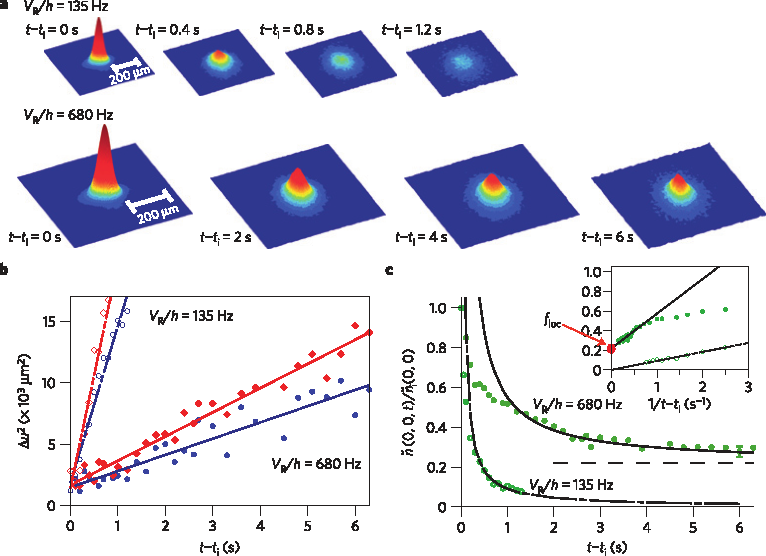
\includegraphics[width=\textwidth]{Fig/Localisation/experience_palaiseau.pdf}
\caption{\textbf{Expérience de Palaiseau.} \textbf{a:} Images expérimentales du nuage de \isotope[87]{Rb} après propagation dans le désordre. Pour un désordre de \SI{135}{\hertz}, le nuage a une dynamique de diffusion. Pour un désordre de \SI{680}{\hertz}, une partie localisée apparaît parmi un fond diffusif lent. \textbf{b:} Évolution temporelle de la taille rms du nuage selon deux axes. La dynamique temporelle linéaire permet de mettre en évidence la composante diffusive du nuage. L'augmentation de l'amplitude du désordre ralentit l'évolution de la composante diffusive du nuage. \textbf{c:} Évolution de la densité atomique au centre du nuage $n(0,t)$. Le régime asymptotique (aux temps longs) permet de déterminer la fraction localisée $\floc$. Figure tirée de \citep{jendrzejewski2012three}.}
\label{fig:experience_palaiseau}
\end{figure}


\paragraph*{Expérience de Florence}
La troisième expérience, réalisée en 2015 à Florence, est la dernière expérience en date cherchant à déterminer le seuil de mobilité avec des atomes ultra-froids \citep{semeghini2015measurement}. Si celle-ci partage de nombreuses similarités avec les expériences précédentes, telles que l'utilisation d'un désordre de type speckle répulsif et l'estimation du seuil de mobilité à l'aide de la mesure de la fraction localisée, cette expérience présente des avantages considérables par rapport à ses prédécesseurs en accordant une attention particulière à la distribution d'énergie des atomes dans le désordre. 

Notamment, un avantage de cette expérience est d'utiliser des atomes de \isotope[39]{K}, bosons dont les interactions sont contrôlables à l'aide d'une résonance de Feshbach. Ainsi, il est possible de charger "quasi-adiabatiquement" les atomes dans le désordre, rendant leur distribution d'énergie beaucoup plus fine que pour les expériences précédentes, utilisant des fermions ou un allumage rapide du désordre. Cette procédure permet de charger les atomes majoritairement dans des états de basses énergies du désordre, illustré figure \ref{fig:experience_florence}.a.I.

En conséquence du processus de chargement quasi-adiabatique, le désordre est ici allumé progressivement et la distribution d'impulsion du nuage $\mathcal{D}_{\mathbf{k}}(\mathbf{k})$ n'est plus associée à l'onde plane $\etat{\mathbf{k}=0}$. Ainsi, la distribution d'énergie des atomes après chargement dans le désordre est donnée par l'équation \ref{eq:fonction_spectrale}, où la distribution d'impulsion est mesurée expérimentalement par la méthode de temps de vol et la fonction spectrale $A(\mathbf{k},E)$ est calculée numériquement. La détermination de la distribution d'énergie nécessite donc de calculer la fonction spectrale pour toutes les impulsions du nuage, dont une représentation est donnée figure \ref{fig:experience_florence}.b.

Une seconde originalité de l'expérience de Florence réside dans sa manière de contrôler l'énergie des atomes chargés dans le désordre. À l'aide d'une modulation de l'amplitude du potentiel pendant une durée $T=\SI{500}{\milli\second}$, les auteurs transfèrent une partie contrôlée des atomes initialement dans un état de basse énergie $E$ vers un état de plus haute énergie $E+\hb\omega$, avec $\omega$ la fréquence de modulation. La distribution d'énergie des atomes après transfert peut alors s'exprimer
\begin{equation}
\mathcal{D}_{\mathrm{E}}(E,\hb\omega)=(1-\alpha)\DE+\alpha \mathcal{D}_{\mathrm{E}}(E-\hb\omega) \text{ ,}
\end{equation}
avec $\alpha$ la probabilité de transfert supposée indépendante de $E$ et $\omega$ dans le cadre de la théorie de la réponse linéaire. Le premier terme correspond à la distribution d'énergie des atomes non transférés, tandis que le second terme correspond quant à lui à la contribution de la partie excitée. Une illustration d'une telle distribution d'énergie est proposée figure \ref{fig:experience_florence}.c.

Avec ce procédé, certains atomes sont excités dans des états d'énergie $E$ supérieure au seuil de mobilité $\Ec$. La fraction localisée est alors obtenue en détectant les atomes restés localisés après \SI{500}{\milli\second} supplémentaires de propagation dans le désordre, voir figure \ref{fig:experience_florence}. Enfin, le seuil de mobilité est déterminé à l'aide de la fraction localisée par le biais de l'équation \ref{eq:fraction_localisee} de manière identique aux expériences précédentes.

\begin{figure}
\centering
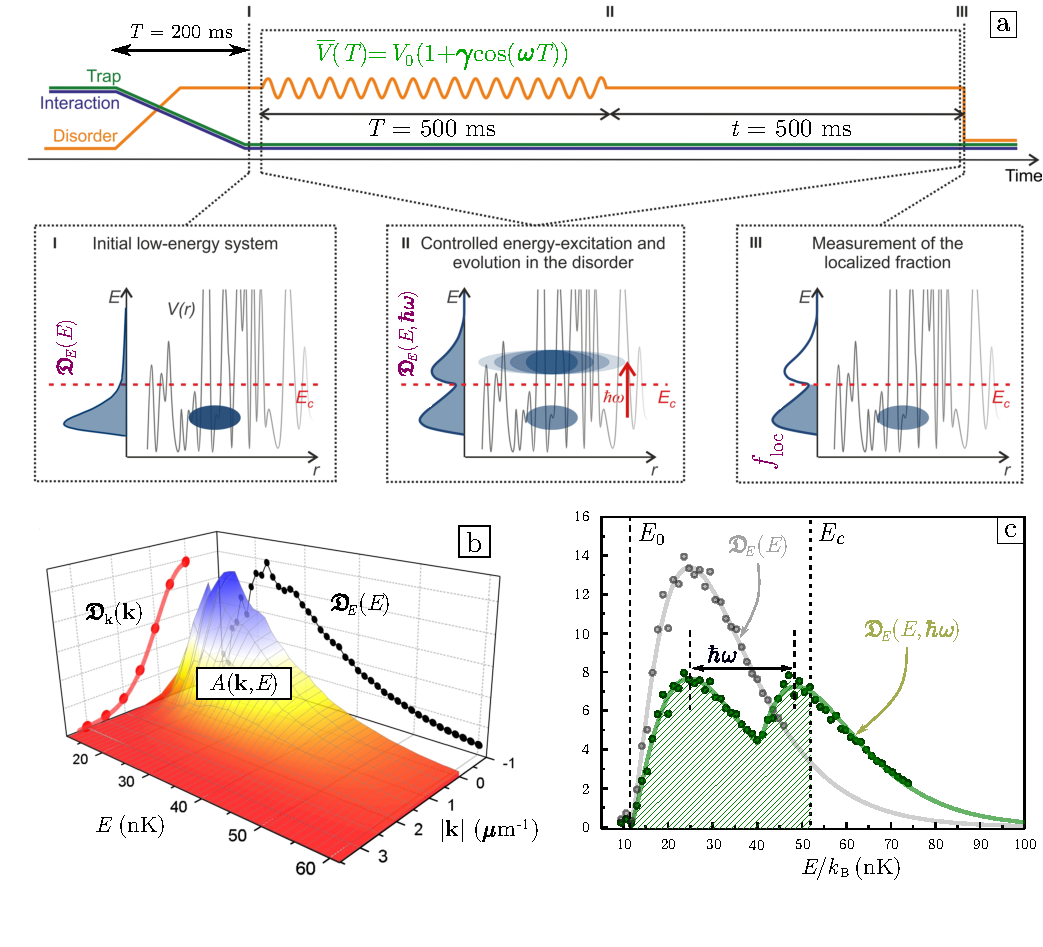
\includegraphics[width=\textwidth]{Fig/Localisation/experience_florence.pdf}
\caption{\textbf{Expérience de Florence.} \textbf{a:} Procédure de mesure du seuil de mobilité. Un état de basse énergie est chargé dans le désordre. Une modulation de l'amplitude du désordre permet de transférer une énergie $\hb \omega$ à certains atomes. La propagation dans le désordre permet d'éliminer la partie diffusive, révélant ainsi la fraction localisée. \textbf{b:} Fonction spectrale $A(\mathbf{k},E)$ calculée numériquement. Celle-ci permet de calculer la distribution d'énergie $\DE$ des atomes dans le désordre à partir de la distribution d'impulsion $\mathcal{D}_{\mathbf{k}}(\mathbf{k})$ des atomes mesurée après le chargement du désordre. \textbf{c:} Exemple de distribution d'énergie des atomes après chargement, modulation et propagation dans le désordre. La courbe grise correspond à la distribution d'énergie après chargement du désordre, la courbe verte correspond à la distribution d'énergie après modulation de l'amplitude du désordre et la surface verte correspond à la fraction des atomes qui sont localisés. Figure tirée de \citep{denechaud2018vers}.}
\label{fig:experience_florence}
\end{figure}

L'expérience de Florence se caractérise donc par une nouvelle approche à la mesure du seuil de mobilité. En particulier, l'attention portée à la sélection de l'énergie des atomes marque le début de l'étude de la transition d'Anderson à \emph{énergie résolue}. Néanmoins, cette expérience comporte des limitations. Notamment, la détermination du seuil de mobilité reste indirecte: il est nécessaire de calculer numériquement la fonction spectrale $A(\mathbf{k},E)$ ainsi que la population transférée. 



\paragraph*{Comparaison aux résultats numériques}
Les trois expériences présentées précédemment \citep{kondov2011three}\citep{jendrzejewski2012three}\citep{semeghini2015measurement} ont toutes cherché à déterminer le seuil mobilité séparant les états localisés des états diffusifs. Comme nous l'avons décrit, celles-ci se sont basées sur la mesure de fractions localisées et sur des estimations de la distribution d'énergie des atomes dans le désordre par le biais de la fonction spectrale.

Un second point commun entre ces expériences réside dans la nature du désordre utilisé: toutes ont utilisé un speckle répulsif, généré à l'aide d'un unique faisceau pour l'expérience d'Urbana Champaign tandis que les expériences de Palaiseau et de Florence ont profité de l'interférence de deux speckles croisés pour générer un désordre quasi-isotrope. 

Dans le cadre de l'étude de l'effet de l'anisotropie du potentiel sur la position du seuil de mobilité pour un potentiel de type speckle, Pasek et al. \citep{pasek2017anderson} ont montré qu'il existe une échelle d'énergie universelle, appelée \emph{énergie de corrélation}, qui permet de renormaliser l'amplitude du désordre $\VR$ et de rendre la prédiction du seuil de mobilité universelle pour un désordre de type speckle répulsif. Cette énergie est définie par
\begin{equation}
\ER=\frac{\hb^2}{m\overline{\sigma}^2} \quad \text{avec} \quad \overline{\sigma}={(\sigma_x \sigma_y \sigma_z)}^{1/3} \text{ ,}
\end{equation}
où les $\sigma_i$ correspondent aux longueurs de corrélation selon chaque direction. À l'aide de cette définition, Pasek et al. ont pu comparer les résultats des différentes expériences à une unique courbe universelle $\Ec/\VR=\mathcal{F}(\VR/\ER)$ obtenue à l'aide de simulations numériques. La compilation de ces résultats est illustrée figure \ref{fig:seuil_mobilite_delande}.


\begin{figure}
\centering
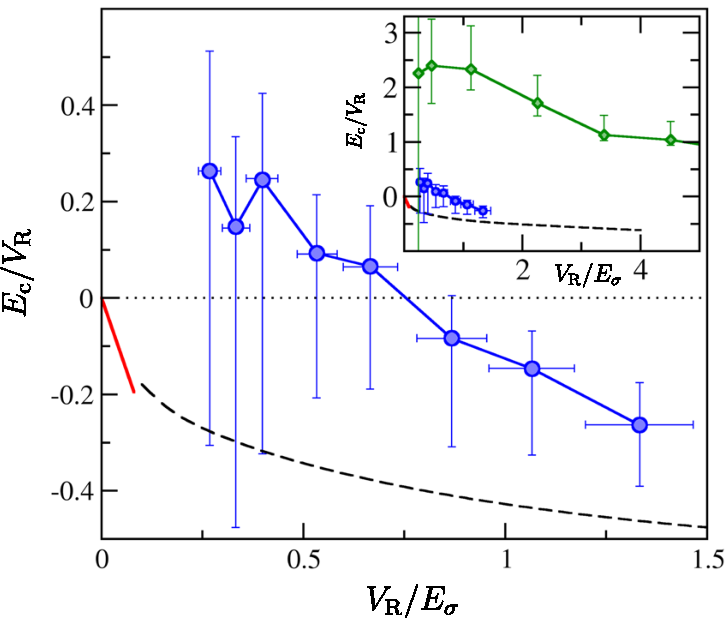
\includegraphics[width=0.6\textwidth]{Fig/Localisation/delande_expvsth.pdf}
\caption{\textbf{Comparaison des résultats expérimentaux à des simulations numériques.} Evolution du seuil de mobilité $\Ec$ en fonction de l'amplitude du désordre $\VR$. La ligne pointillée noire correspond à la prédiction universelle $\Ec/\VR=\mathcal{F}(\VR/\ER)$. Les résultats de l'expérience de Palaiseau sont représentés par la ligne rouge, tandis que les résultats de l'expérience de Florence sont reportés par des points bleus. Les résultats de l'expérience d'Urbana Champaign sont représentés par des points verts dans l'encart, représentant la même figure en échelle dilatée. Figure tirée de \citep{pasek2017anderson}.}
\label{fig:seuil_mobilite_delande}
\end{figure}

Les résultats de l'expérience d'Urbana Champaign, dont les interprétations sont fortement controversées, sont représentés en points verts dans l'encart et montrent un désaccord significatif avec les résultats numériques. En particulier, les résultats expérimentaux surestiment fortement le seuil de mobilité en raison du temps très court de propagation dans le désordre et de l'hypothèse \ref{eq:hypothese_urbana_champaign} sur la fonction spectrale. L'expérience de Palaiseau, dont les résultats sont représentés en rouge, semblent en accord quantitatif avec les prédictions numériques mais sont limités au régime de désordre faible, ou encore de désordre quantique comme nous le décrirons dans les chapitres \ref{ch:TauS_PRL} et \ref{ch:TauS_NJP}. Rappelons aussi que cette estimation du seuil de mobilité est très indirecte, car basée sur une mesure de la fraction localisée et une estimation numérique de la fonction spectrale. Les résultats de l'expérience de Florence sont représentés en bleu et semblent en accord qualitatif avec les résultats numériques. Néanmoins, les données expérimentales semblent légèrement surestimer le seuil de mobilité, probablement en raison d'un temps de propagation trop court dans le désordre ou du calcul de la distribution d'énergie. L'ensemble de ces résultats montre donc qu'il est fondamental d'avoir des temps de propagation dans le désordre de plusieurs secondes afin de ne pas surestimer le seuil de mobilité.




\subsection{Nécessité d'une spectroscopie pour sonder le régime critique}
\label{sc:spectroscopie_transition}
Les trois expériences citées précédemment reposent sur une détermination indirecte du seuil de mobilité, et nécessitent une estimation numérique de la distribution d'énergie $\DE$, capitale pour calculer le seuil de mobilité. Comme nous l'avons vu, l'obtention de la distribution d'énergie passe par l'intermédiaire de la fonction spectrale $A(\mathbf{k},E)$, qu'aucune de ces expériences n'a mesurée. 

De plus, dans le cas d'une estimation fiable de la fonction spectrale, la coexistence d'une phase localisée et d'une phase diffusive témoigne d'une large distribution d'énergie, rendant l'étude du régime critique et plus particulièrement des exposants critiques de la transition impossible.

Il apparaît donc que, dans l'optique de sonder le régime critique, il est important de maîtriser le paramètre de contrôle de la transition d'Anderson, c'est à dire l'énergie $E$ de l'onde. Pour cela, une nouvelle approche expérimentale résolue en énergie s'avère nécessaire, approche pour laquelle il serait possible de peupler sélectivement les états $\etat{E}$ d'énergie bien définie du désordre. La méthode proposée par notre équipe pour l'étude la transition d'Anderson consiste donc à réaliser une spectroscopie du désordre.





Un protocole expérimental de spectroscopie de la transition d'Anderson tel que celui envisagé par notre équipe serait proche de celui de l'expérience de Florence: un état initial $\etat{i}$ libre de faible énergie est transféré sélectivement dans un état propre $\etat{E_\alpha}$ du désordre dans un premier temps, puis une expansion de plusieurs secondes dans le désordre permet de caractériser cet état en terme de localisation ou de diffusion. 




\begin{figure}
\centering
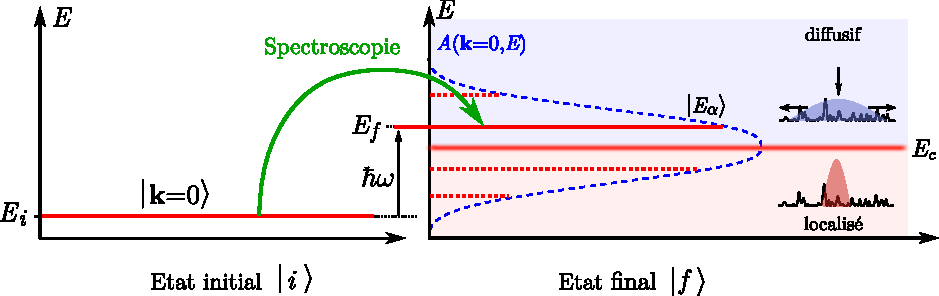
\includegraphics[width=\textwidth]{Fig/Localisation/spectroscopie_anderson.pdf}
\caption{\textbf{Approche spectroscopique de l'étude la transition d'Anderson.} Dans l'optique de sonder la transition d'Anderson, il est nécessaire de peupler sélectivement les différentes énergies du désordre. Pour cela, l'onde est préparée dans un état insensible au désordre, puis est transférée à une énergie bien définie dans le désordre à l'aide d'une spectroscopie. Enfin, l'expansion du nuage permet de caractériser l'énergie adressée en terme de localisation ou de diffusion.}
\label{fig:spectroscopie_anderson}
\end{figure}


Depuis ces premiers résultats expérimentaux novateurs, une telle spectroscopie a pu être implémentée sur notre expérience en tant que preuve de principe. Cette méthode spectroscopique a pu être validée en s'intéressant au taux de transfert entre l'état initial libre et les états habillés par le désordre, qui s'avère être une mesure directe de la fonction spectrale $A(\mathbf{k}=0,E)$ (le protocole de mesure sera explicité dans le chapitre \ref{ch:TauS_NJP}) \citep{volchkov2018measurement}.

Cette méthode spectroscopique répond alors à deux problématiques essentielles: celle-ci démontre notre capacité à adresser des énergies bien définies dans le désordre, donc de contrôler la distribution d'énergie des atomes dans le désordre, et de mesurer les fonctions spectrales dont la connaissance est capitale pour l'étude de la transition d'Anderson.
 
Cependant, différentes limitations expérimentales ont empêché de procéder aux mesures d'expansion nécessaires à la caractérisation des différents états d'énergie en terme de localisation. Les deux principales sources de limitation identifiées seront discutées dans les chapitres \ref{ch:new_exp} et \ref{ch:Speckle}.


\begin{comment}

%%% mettre les performances ??? ceci peut être intéressant ? chercher données ? Freedman peut être ?
\begin{figure}[h!]
	\centering
	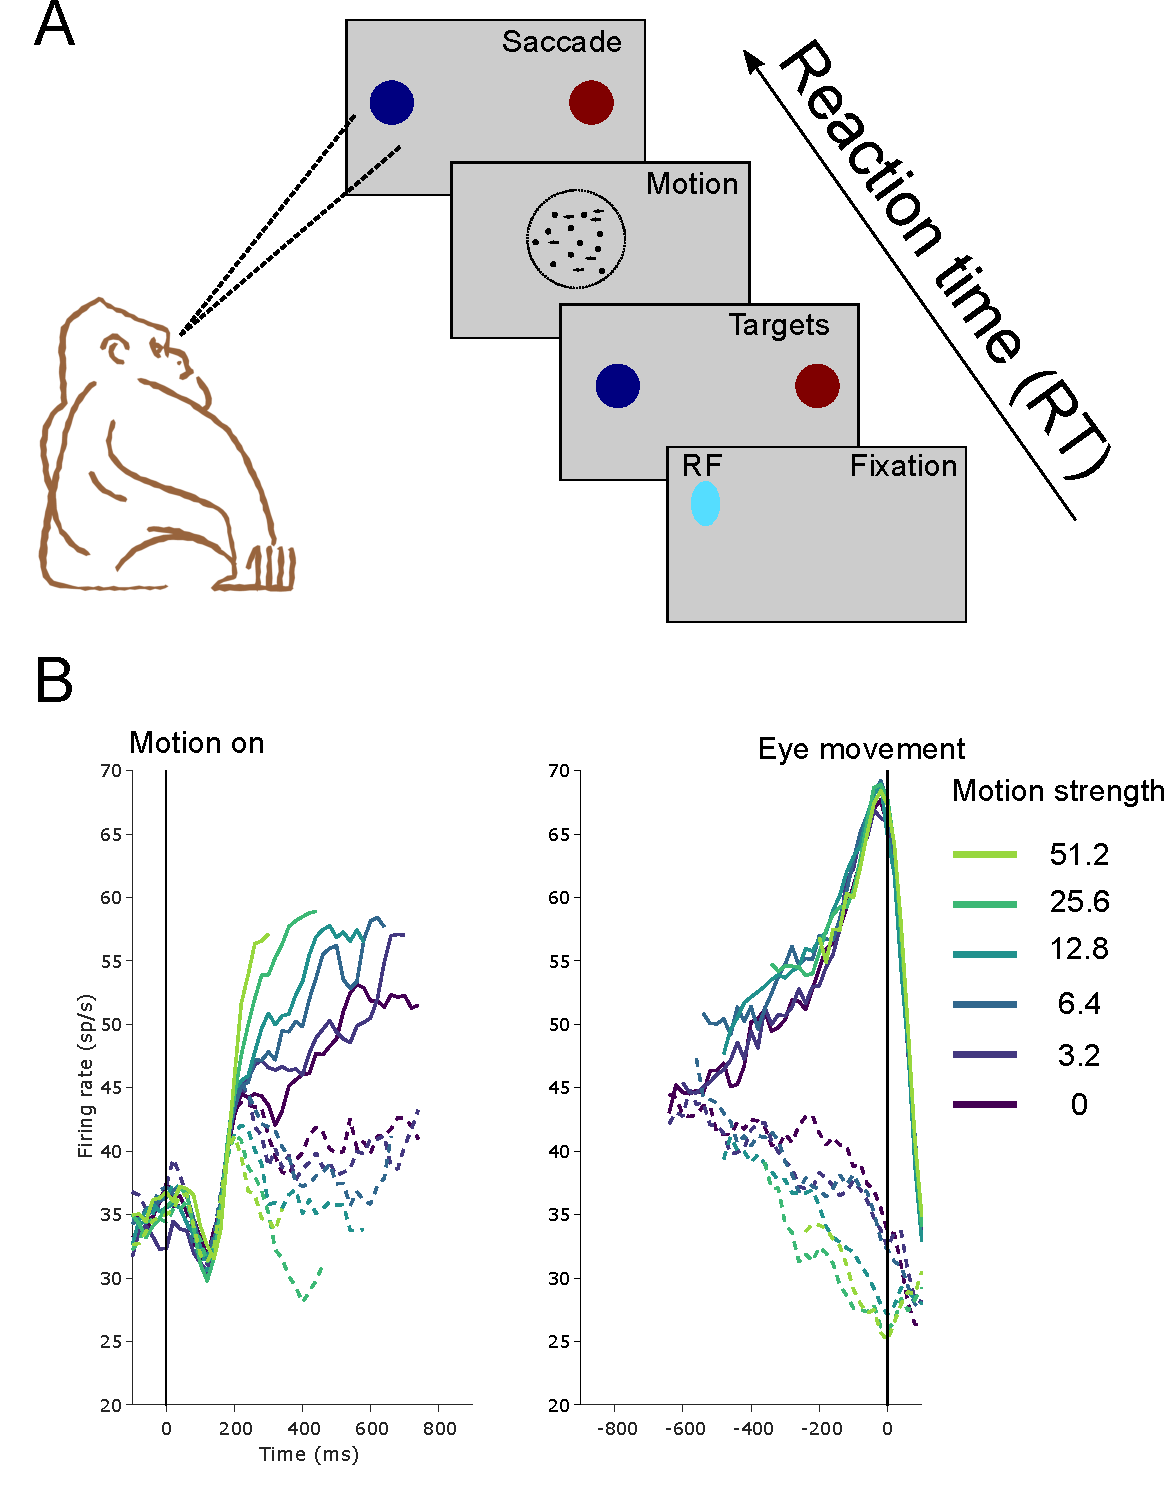
\includegraphics[width=0.8\linewidth]{Fig/Chapter1/RDM.pdf}
	\caption{{\bf Reaction time version of the random dot motion discrimination task.}   (A) The monkey views a set of dots moving across the screen and decides the net direction of movement. The decision is indicated by a saccadic eye movement to one the two peripheral target. The light blue field corresponds to the receptive field of one of the recorced LIP neurons. The monkey is the figure was obtained using the AutoDraw software. (B) Response of LIP neurons during decision. The data are from~\cite{roitman2002response} and are publicly available. The average firing rate of $54$ LIP neurons is shown for $6$ degrees of difficulty. The firing rate are grouped by motion difficulty and direction of choice (dashed line corresponding to choice out of the receptive field of the neuron). The left panel represents the average firing rate during decision formation starting from motion onset. The right panel shows the average firing rate centered at the time of the eye movement.
	}
	\label{fig:RDM}
\end{figure}
%% REF AutoDraw ??,

\end{comment}
%\stopcontents

\usechapterimagetrue
\chapterimage{Fig/BEC_manip/BEC.pdf}
%\part{Transport d'atomes ultrafroids dans un speckle} 
\chapter{Production d'ondes de matière}
\label{ch:BEC_manip}
%\begin{tikzpicture}[remember picture, overlay]
%\node[anchor=north east,inner sep=0pt] at (current page.north east) {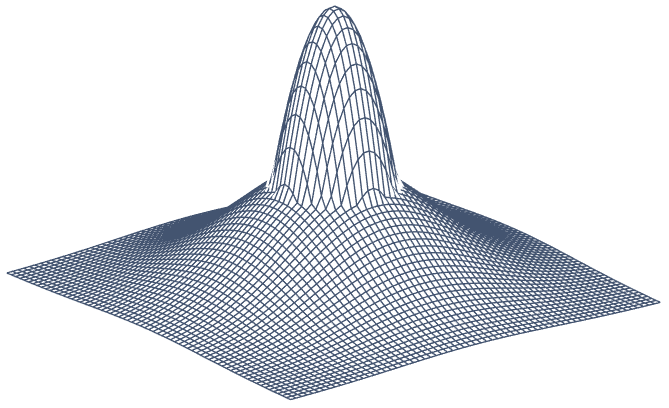
\includegraphics[scale=0.6]{Fig/BEC_manip/header.png}};
%\end{tikzpicture}

Dans la partie précédente, nous nous sommes concentrés sur la physique des atomes ultrafroids dans le désordre. En particulier, nous avons mis en évidence le fait que l'approche des atomes ultrafroids constitue une plateforme idéale pour l'étude de la propagation d'ondes dans un milieu désordonné, plateforme déjà éprouvée par l'observation de la localisation d'Anderson d'ondes de matières dans un désordre optique. 

À présent, concentrons-nous sur la description de l'un des deux éléments-clé de la propagation d'ondes dans le désordre: notre source d'ondes de matière. Le second élément, notre désordre optique, sera quant à lui présenté dans le chapitre \ref{ch:Speckle}.

Dans ce chapitre, nous nous attacherons donc à définir ce qu'est un condensat de Bose-Einstein puis nous décrirons ses principales propriétés. Dans un second temps, nous nous intéresserons aux outils dont nous disposons pour manipuler les atomes, puis nous terminerons en présentant la manière dont ces outils sont implémentés sur notre dispositif expérimental. 

\section{Condensation de Bose-Einstein}
Commençons par décrire ce qu'est un condensat de Bose-Einstein. Le phénomène de condensation a été prédit par Albert Einstein dans les années 1920 en s'appuyant sur les travaux de Satyendranath Bose traitant des statistiques quantiques pour des particules plus tard appelées \emph{bosons}. Il a cependant fallu attendre les années 1960 et le développement des premiers lasers pour voir émerger les premières techniques de manipulation d'atomes. La mise au point de telles technologies a d'ailleurs valu le prix Nobel à ses principaux architectes Claude Cohen-Tannoudji, Steven Chu et William D. Phillips en 1997. Enfin, le premier condensat de Bose-Einstein gazeux de \isotope[87]{Rb} a été obtenu par l'équipe de Eric Cornell et Carl Wieman \citep{anderson1995observation}, rapidement suivi par un condensat de \isotope[23]{Na} obtenu par Wolfgang Ketterle \citep{davis1995bose}. Ces travaux ont été récompensés par le prix Nobel de 2001.

Depuis, des condensats de Bose-Einstein ont été produits pour un grand nombre d'espèces chimique, pour des atomes comme pour des molécules. Aujourd'hui, les condensats sont couramment utilisés comme outils à des fins différentes, aussi leurs propriétés ont pu être abondamment étudiées par le passé et restent l'objet de l'investigation de plusieurs groupes dans le monde. Ainsi, nous n'en présenterons ici que les propriétés essentielles à la suite de ce manuscrit.

\subsection{Statistique de Bose-Einstein}
Le phénomène de condensation de Bose-Einstein trouve son origine dans la statistique de Bose-Einstein. Celle-ci se différencie de la statistique classique de Boltzmann dans le formalisme grand-canonique donnée par:
\begin{equation}
N_{\mathbf{n}}=g_{\mathbf{n}} \exp{\left( -(E_{\mathbf{n}}-\mu)/\kB T \right)} \text{ ,}
\end{equation}
pour un gaz de $N$ particules à l'équilibre thermique, avec $N_{\mathbf{n}}$ le nombre moyen d'atomes présents dans l'état d'énergie $E_{\mathbf{n}}$ et de dégénérescence $g_{\mathbf{n}}$, $\mu$ le potentiel chimique, $T$ la température et $\kB$ la constante de Boltzmann. L'origine de cette différence provient de l'indiscernabilité des particules: dans le cadre de la physique classique, les particules identiques sont discernables, c'est à dire qu'il est possible "d'étiqueter" les particules et de suivre leurs mouvements individuels.
Dans le cadre de la mécanique quantique, une telle approche n'est pas possible car les particules sont décrites par des fonctions d'onde, étalées dans l'espace. Lors de collisions de particules identiques, le recouvrement de leur fonction d'onde fait qu'il est impossible de déterminer les trajectoires suivies par les particules. L'indiscernabilité des particules dans le cadre de la mécanique quantique est donc essentielle.

\begin{figure}
\centering
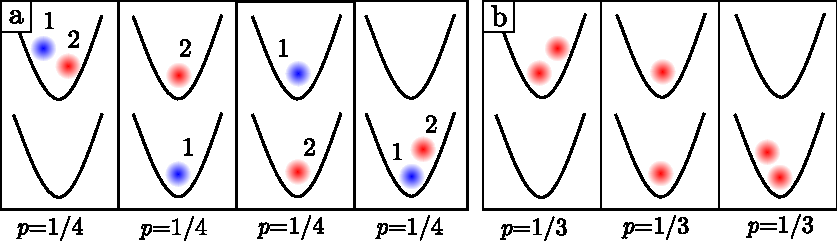
\includegraphics[width=\textwidth]{Fig/BEC_manip/stat_bose.pdf}
\caption{\textbf{a: Répartition de deux particules discernables numérotées 1 et 2 sur deux niveaux d'énergie.} Quatre configurations sont possibles. \textbf{b: Répartition de deux particules indiscernables sur deux niveaux d'énergie.} Dans le cas où ces particules peuvent se trouver dans le même état (bosons), trois configurations sont alors possibles.}
\label{fig:stat_bose}
\end{figure}

Considérons alors le cas simple de la répartition de deux particules sur deux niveaux d'énergie. Dans le cadre de la physique classique, il est possible d'attribuer un numéro à chaque particule, et il on peut placer chaque particule dans n'importe quel niveau d'énergie. Il existe alors quatre configurations que l'on supposera équiprobables, chacune de probabilité $p=1/4$ (voir figure \ref{fig:stat_bose}a). L'approche quantique, dans laquelle il n'est pas possible de discerner les particules, restreint le nombre de possibilités à trois et donc la probabilité de chacune des configurations est alors de $p=1/3$ (voir figure \ref{fig:stat_bose}b). Calculons maintenant la probabilité que deux particules soient dans le même état. En physique classique, cette probabilité est de $p=2/4=1/2$, tandis qu'en mécanique quantique, celle-ci est de $p=2/3$. On s'attend alors à ce que l'indiscernabilité des particules en mécanique quantique modifie la statistique de Boltzmann en favorisant l'agrégation de particules dans le même état \footnote{Ce raisonnement est valable pour des particules bosoniques, qui peuvent se retrouver dans le même état quantique. Pour des particules fermioniques, qui ne peuvent pas occuper le même état quantique, les statistiques en sont donc profondément changées. En guise d'illustration, la seule configuration possible de la figure \ref{fig:stat_bose}b pour des fermions est la seconde configuration.}.

\paragraph*{Condensation de Bose-Einstein}
Considérons alors le cas d'un gaz de $N$ bosons identiques dans un piège harmonique:
\begin{equation}
V(x,y,z)=\frac{1}{2}m \omega_x^2 x^2 + \frac{1}{2}m \omega_y^2 y^2 + \frac{1}{2}m \omega_z^2 z^2 \text{ ,}
\label{eq:piege_harmonique}
\end{equation}
où $m$ correspond à la masse des particules, et les $\omega_i$ correspondent aux fréquences de piégeage dans chaque direction de l'espace. Les énergies $E_{\mathbf{n}}$ sont donc celles des états liés
\begin{equation}
E_{\mathbf{n}}=\left(n_x+\frac{1}{2}\right) \hb \omega_x + \left(n_y+\frac{1}{2}\right) \hb \omega_y + \left(n_z+\frac{1}{2}\right) \hb \omega_z \quad \text{avec}\quad \mathbf{n}=\lbrace n_x,n_y,n_z\rbrace \text{ .}
\end{equation}

On peut alors montrer que le nombre moyen de particules est donné par la distribution de Bose-Einstein \footnote{Pour un gaz de $N$ fermions identiques, le nombre moyen de particules est donné par la distribution de Fermi-Dirac $ N_{\mathbf{n}}=\frac{g_{\mathbf{n}}}{\exp{\left( (E_{\mathbf{n}}-\mu)/\kB T\right)}+1}$.} \citep{diu1989elements}:
\begin{equation}
N_{\mathbf{n}}=\frac{g_{\mathbf{n}}}{\exp{\left( (E_{\mathbf{n}}-\mu)/\kB T \right)}-1} \text{ .}
\end{equation}
Une condition de validité de cette équation est que le potentiel chimique $\mu$ soit plus petit que l'énergie $E_{\mathbf{0}}$ du niveau de plus basse énergie, appelé niveau fondamental. Autrement, le nombre moyen de particules du niveau fondamental serait négatif (et cela impliquerait que la totalité du réservoir de particules vienne se déverser dans le niveau fondamental). Il est donc nécessaire que $\mu < E_{\mathbf{0}}$. Une conséquence remarquable cette condition est que la population totale des états excités est bornée par:
\begin{equation}
N_e(\mu,T)=\sum_{\mathbf{n}\neq\mathbf{0}} N_{\mathbf{n}} \leq \sum_{\mathbf{n} \neq \mathbf{0}} \frac{g_{\mathbf{n}}}{\exp{\left( (E_{\mathbf{n}}-E_{\mathbf{0}})/\kB T \right)}-1} \text{ .}
\end{equation}
Ainsi, chaque particule supplémentaire peuplera forcément l'état fondamental. On a donc ici le moyen d'accumuler un grand nombre de particules dans le même état quantique. La condensation de Bose-Einstein correspond, par définition, à cette accumulation d'un nombre macroscopique de particules dans l'état fondamental. C'est dans ce régime que les effets quantiques se manifestent, toutes ces particules partageant alors le même état quantique. Afin d'obtenir de tels effets, il est nécessaire que les fonctions d'onde des particules individuelles se recouvrent, c'est à dire que l'extension typique d'un paquet d'onde soit plus grande que la distance moyenne entre particules. Cette extension typique est donnée par la longueur d'onde thermique de de Broglie $\Delta x \sim \ldb$, qui correspond à la taille typique d'un paquet d'onde quantique dont la largeur de la distribution en impulsion est donnée par la température. Elle s'exprime \citep{diu1989elements}
\begin{equation}
\ldb=\sqrt{\frac{2\pi \hb^2}{m \kB T}} \text{ ,}
\end{equation}
avec m la masse de la particule, un atome de \isotope[87]{Rb} dans le cas de notre expérience. La distance inter-particules dans un piège est estimée à partir de la densité de particules $d \sim n^{-1/3}$. On peut alors formuler le critère phénoménologique suivant:
\begin{equation}
n \ldb^3 \gtrsim 1 \text{ .}
\label{eq:critere_condensation}
\end{equation}
La quantité $n \ldb^3$ est appelée \emph{densité dans l'espace des phases}. Tout l'enjeu des expériences d'atomes ultrafroids est d'arriver à augmenter la densité dans l'espace des phases afin de franchir le seuil donné par l'équation \ref{eq:critere_condensation}. Cette condition peut se réécrire en terme de \emph{température critique}:
\begin{equation}
T_{\mathrm{C}}\sim \frac{\hb \overline{\omega}}{\kB}N^{1/3} \text{ ,}
\label{eq:temperature_critique}
\end{equation}
où $\overline{\omega}=(\omega_x \omega_y \omega_z)^{1/3}$ est la fréquence moyenne du piège. Cette température critique est de l'ordre de quelques centaines de nanokelvin pour les expériences typiques d'atomes ultra-froids.





\subsection{Propriétés d'un condensat de Bose-Einstein}
\label{sc:propriete_BEC}
En dessous de la température critique \ref{eq:temperature_critique}, les atomes s'accumulent dans l'état fondamental du piège. Il en résulte une forte augmentation de la densité, si bien qu'on ne peut plus négliger les interactions entre particules. Dans le cas d'un gaz suffisamment dilué, ce que l'on considèrera dans la suite, les interactions entre atomes peuvent être traitées comme des collisions à basse énergie, c'est à dire des collisions uniquement dans l'onde \emph{s}. Le potentiel d'interaction est alors celui de contact, donné par $U(\mathbf{x}_1-\mathbf{x}_2)=g\delta(\mathbf{x}_1-\mathbf{x}_2)$. Le paramètre $g$, qui caractérise la force des interactions, est donné par $g=\frac{4 \pi \hb^2}{m}a_{\mathrm{s}}$, avec $a_{\mathrm{s}}$ la longueur de diffusion, et ne dépend que de ce paramètre. Ce régime dilué est atteint lorsque $na_{\mathrm{s}}^3\ll 1$\footnote{Dans ce régime, la distance inter-atomique est plus grande que la portée des interactions. Ainsi, les atomes ne voient pas le détail du potentiel d'interaction avec leur voisin, et donc il est possible d'approximer ce potentiel par un potentiel de contact.}. Pour le \isotope[87]{Rb}, cette longueur de diffusion vaut \SI{100}{\bohr}, avec \SI{}{\bohr} le rayon de Bohr. La longueur de diffusion étant positive, les interactions sont donc répulsives pour notre atome.

On peut écrire l'équation de Schrödinger pour l'état fondamental en tenant compte de ce terme d'interaction entre particules. La description en champ moyen du condensat est alors donnée par l'équation de Gross-Pitaevskii (aussi connue sous le nom d'\emph{équation de Schrödinger non-linéaire}):
\begin{equation}
\left[ -\frac{\hb^2}{2m}\Delta + V(\mathbf{x}) + g\left|\phi_0(\mathbf{x})\right|^2 \right] \phi_0(\mathbf{x}) = \mu \phi_0(\mathbf{x}) \text{ ,}
\label{eq:gross_pitaevskii}
\end{equation}
où $\phi_0(\mathbf{x})$ est la fonction d'onde macroscopique du condensat et $\mu$ est le potentiel chimique. La densité d'atomes est donnée par $n(\mathbf{x})=\left| \phi_0(\mathbf{x}) \right|^2$. Ainsi, la fonction d'onde du condensat $\phi_0(\mathbf{x})$ est normalisée pour donner le nombre de particules dans le condensat $\Nzero=\int{\diff\mathbf{x} \: \left| \phi_0(\mathbf{x}) \right|^2}$.

Le premier terme de gauche décrit l'énergie cinétique, le second le terme d'énergie potentielle provenant du piège, et le dernier décrit l'énergie d'interaction entre particules%, proportionnelle à la densité locale $n(\mathbf{x})$
. La somme de ces énergies donne le potentiel chimique $\mu$, qui correspond à l'énergie qu'il faut fournir pour rajouter une particule supplémentaire au système de $\Nzero$ particules.




\paragraph*{Régime de Thomas-Fermi}
Considérons le cas d'un condensat comportant un grand nombre de particules $\Nzero$. L'énergie cinétique totale du condensat varie avec $\Nzero$ de manière linéaire: $\mean{E_{\mathrm{k}}}\propto \Nzero$. L'énergie totale d'interaction varie quant à elle en $E_{\mathrm{int}}\propto \Nzero^2$. Pour un nombre suffisamment grand de particules, il devient possible de négliger le terme d'énergie cinétique dans l'équation de Gross-Pitaevskii stationnaire: il s'agit du régime de Thomas-Fermi.
Dans ce cas, le profil de densité s'écrit
\begin{equation}
n(\mathbf{x})=\left\{
					\begin{array}{ll}
						(\mu-V(\mathbf{x}))/g &\quad \text{lorsque} \quad \mu>V(\mathbf{x}) \text{ ,}\\
						0 &\quad \text{sinon.}
					\end{array} 
				\right.
\end{equation}
Le profil de densité est donc une parabole inversée de rayons $R_{\mathrm{TF},i}=\sqrt{\frac{2\mu}{m\omega_i^2}}$ en considérant le piège harmonique de l'équation \ref{eq:piege_harmonique}.
Ces rayons de Thomas-Fermi ont été déterminés par la condition $n(\mathbf{x})=0$. Il est intéressant de noter que le potentiel effectif vu par une particule $V_{\mathrm{eff}}(\mathbf{x})=V(\mathbf{x})+gn(\mathbf{x})$ est constant sur l'ensemble du condensat:
\begin{equation}
V_{\mathrm{eff}}(\mathbf{x})= \left\{
									\begin{array}{ll}
										\mu &\quad \text{lorsque} \quad \mu>V(\mathbf{x}) \text{ ,}\\
										V(\mathbf{x}) &\quad \text{sinon.}
									\end{array}
							\right.
\end{equation}
L'énergie d'un atome est donc constante sur l'ensemble du condensat et est donnée par le potentiel chimique. $\mu$ correspond alors à l'échelle d'énergie au-delà de laquelle le condensat est perturbé par le potentiel. Il est possible d'obtenir une expression pour le potentiel chimique \citep{pethick2008bose}: 
\begin{equation}
\mu=\frac{1}{2} \left( 15a \Nzero \hb^2 \overline{\omega}^3 \right) ^{2/5} m^{1/5} \text{ ,}
\end{equation}
qui vaut environ $\mu/h\approx\SI{40}{\hertz}$ pour notre expérience.

\begin{figure}
\centering
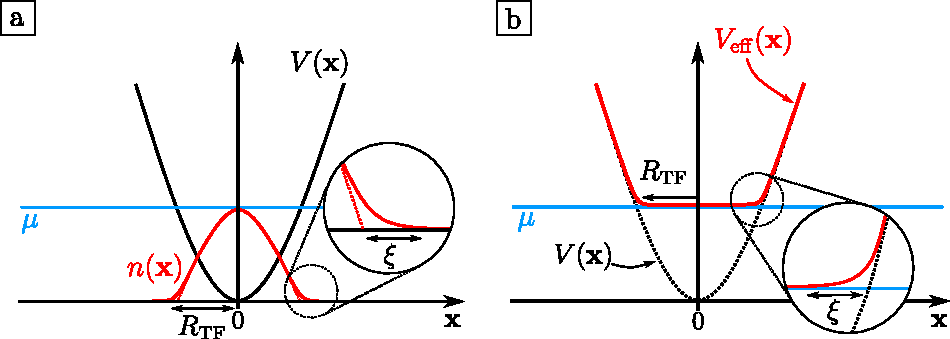
\includegraphics[width=\textwidth]{Fig/BEC_manip/thomas_fermi.pdf}
\caption{\textbf{a: Profil de densité dans le régime de Thomas-Fermi.} La densité est une parabole inversée, liée à la forme parabolique du potentiel. Sur les bords du condensat, la densité s'écarte de la parabole sur une longueur typique appelée longueur de cicatrisation \protect\footnotemark. \textbf{b: Potentiel effectif ressenti pour des particules individuelles.} Ce potentiel effectif suit la forme du potentiel externe, et l'effet des interactions à l'intérieur du condensat écrante le potentiel externe par le potentiel chimique.}
\label{fig:thomas_fermi}
\end{figure}
\footnotetext{En réalité, l'approximation de Thomas-Fermi décrit bien les zones à l'intérieur des condensats, cependant, il existe une petite région sur les bords du condensat où la densité est faible, et donc l'énergie cinétique ne peut plus être négligée devant l'énergie d'interaction. Cette échelle de longueur s'appelle la longueur de cicatrisation, et est donnée par $\xi=\sqrt{\frac{\hb^2}{n_{\mathbf{0}} mg}}$ avec $n_{\mathbf{0}}=N_{\mathbf{0}}/R_{\mathrm{TF}}^3$ la densité moyenne du condensat. $\xi$ représente donc la longueur sur laquelle le potentiel chimique n'écrante pas le potentiel externe.}








\section{Processus d'interaction lumière-matière}
Précédemment, nous avons brièvement présenté le phénomène de condensation de Bose-Einstein ainsi que les principales propriétés d'un condensat. En particulier, nous avons identifié $n \ldb^3 \gtrsim 1$ comme un critère de condensation, impliquant l'obtention de nuages denses à très basse température. Il s'agit donc de la ligne à atteindre sur notre dispositif. Dans cette partie, nous allons présenter les différents outils de manipulation d'atomes dont nous disposons, tels que des champs magnétiques, des champs lasers ou encore des radio-fréquences, afin d'obtenir la condensation d'un nuage de rubidium \isotope[87]{Rb}.

\subsection{Le rubidium \isotope[87]{Rb}}
\label{sc:Rb87}
Comme déjà mentionné plusieurs fois, l'espèce atomique utilisée sur notre expérience est le rubidium \isotope[87]{Rb}, le second isotope le plus fréquent après le rubidium \isotope[85]{Rb} (l'abondance naturelle du \isotope[87]{Rb} est de 27.8\%). Il s'agit d'un alcalin bosonique (il possède donc un seul électron de valence) avec un spin nucléaire $\mathbf{I}=3/2$. Historiquement, le \isotope[87]{Rb} est l'atome ayant été condensé en premier \citep{anderson1995observation} en raison du développement rapide des technologies laser à \SI{780}{\nano\metre}, cet atome possédant une transition optique cyclante à cette longueur d'onde dans sa raie $D$. 

La raie $D$ est en réalité composée de deux transitions: la raie $D_1$ correspondant à la transition $5^2S_{1/2}\rightarrow5^2P_{1/2}$ à \SI{795}{\nano\metre}, et la raie $D_2$ correspondant à la transition $5^2S_{1/2}\rightarrow5^2P_{3/2}$ à \SI{780}{\nano\metre}. Sauf mention contraire, nous n'utiliserons que la raie $D_2$ dans la suite de ce manuscrit, la plupart de nos fréquences optiques se trouvant autour de \SI{780}{\nano\metre}. Le choix de l'atome de rubidium est aussi dû à ses bonnes propriétés. En particulier, sa longueur de diffusion $a_{\mathrm{s}}=\SI{5.3}{\nano\metre}$ résulte en des taux de collisions relativement élevés, permettant une thermalisation rapide du nuage. 

La structure hyperfine de l'état fondamental $5^2S_{1/2}$ consiste en deux niveaux hyperfins dégénérés $\etatF{1}{}$ et $\etatF{2}{}$ séparés de $\deltahf=\SI{6.835}{\giga\hertz}$. Chacun de ces états est composé de $2F+1$ sous-états Zeeman $\etat{F,\mf}$. Une vue simplifiée de cette structure est donnée figure \ref{fig:Rb87}, et un tableau récapitulatif des principales grandeurs du \isotope[87]{Rb} peut être trouvé table \ref{tbl:Rb87}.

%\renewcommand{\arraystretch}{1.1}
\arrayrulecolor{white}
\setlength{\arrayrulewidth}{0.5mm}
\begin{table}[!ht]
\begin{center}
{\rowcolors{2}{white}{MainColor!10}
\begin{tabular}{ c|c|c }
%\hline
{\color{MainColor} \textbf{Quantité physique}} & {\color{MainColor}\textbf{Symbole}} & {\color{MainColor}\textbf{Valeur}} \\
%\hline
Masse & $m$ & \SI{1.44e-25}{\kilogram} \\
%\hline
Fréquence de transition $D_2$ & $\omega_0$ & $2\pi \times \SI{384.230}{\tera\hertz}$ \\
%\hline
Longueur d'onde dans le vide ($D_2$) & $\lambda_{\mathrm{0}}$ & \SI{780.241}{\nano\metre} \\
%\hline
Largeur naturelle de la transition $D_2$ & $\Gamma$ & $2\pi \times \SI{6.07}{\mega\hertz}$ \\
%\hline
Fréquence de transition $D_1$ & $\omega_{D_1}$ & $2\pi \times \SI{377.107}{\tera\hertz}$ \\
%\hline
Longueur d'onde dans le vide ($D_1$) & $\lambda_{D_1}$ & \SI{794.979}{\nano\metre} \\
%\hline
Largeur naturelle de la transition $D_1$ & $\Gamma_{D_1}$ & $2\pi \times \SI{5.75}{\mega\hertz}$ \\
%\hline
Séparation hyperfine & $\deltahf$ & \SI{6.834682611}{\giga\hertz} \\
%\hline
Moment cinétique nucléaire & $\mathbf{I}$ & 3/2 \\
%\hline
Facteur de Landé électronique & $g_{\mathrm{S}}$ & 2.002319 \\
%\hline
Facteur de Landé orbital & $g_{\mathrm{L}}$ & 0.999993\\
%\hline
Facteur de Landé nucléaire & $g_{\mathrm{I}}$ & \num{-0.9951414e-3} \\
%\hline
Intensité de saturation & $I_{\mathrm{sat}}$ & \SI{1.67}{\milli\watt\per\centi\metre^2} \\
%\hline
Longueur de diffusion & $a_{\mathrm{s}}$ & \SI{5.3}{\nano\metre} \\
%\hline
\end{tabular}}
\end{center}
\caption{Tableau récapitulatif des grandeurs physiques du rubidium \isotope[87]{Rb} que nous utiliserons dans la suite. Ces valeurs sont tirées de \citep{steck2001rubidium}.}
\label{tbl:Rb87}
\end{table}

\begin{figure}
\centering
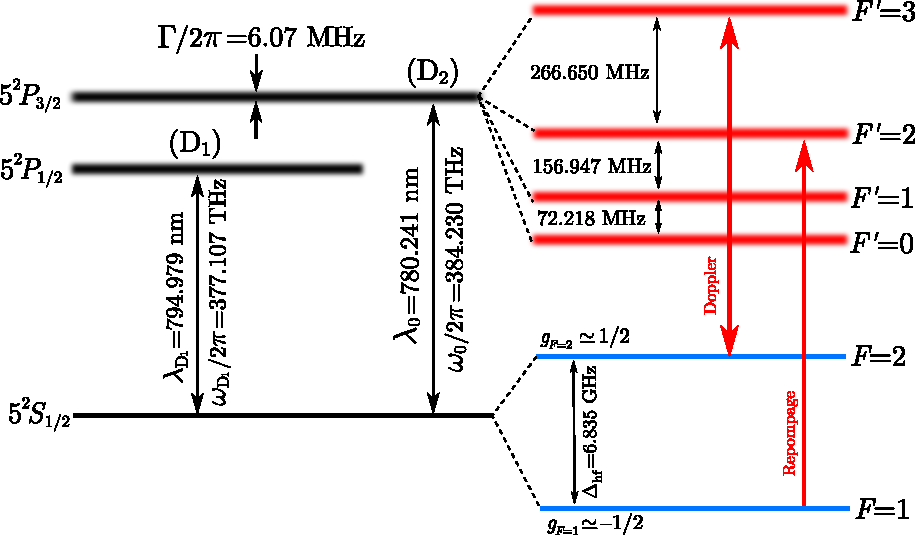
\includegraphics[width=0.8\textwidth]{Fig/BEC_manip/Rb87.pdf}
\caption{\textbf{Structure de la raie $D$ du rubidium \isotope[87]{Rb}.} Celle-ci est composée de deux transitions, la $D_1$ à \SI{795}{\nano\metre}, et la transition $D_2$ à \SI{780}{\nano\metre} que nous utilisons sur l'expérience. L'état fondamental $5^2S_{1/2}$ est dégénéré en deux sous-niveaux hyperfins séparés d'une énergie $h \deltahf$ avec $\deltahf=\SI{6.835}{\giga\hertz}$.}
\label{fig:Rb87}
\end{figure}

\subsection{Potentiel magnétique}
Commençons par décrire l'interaction d'un atome de rubidium avec un champ magnétique statique. Ces champs magnétiques sont couramment utilisés dans les expériences d'atomes ultra-froids pour réaliser des pièges conservatifs à l'aide champs inhomogènes (après un refroidissement laser par exemple). En particulier, l'expérience de Stern \& Gerlach montre que la force appliquée aux atomes par un gradient de champ magnétique dépend de l'état interne de l'atome. Explicitons cela.

Le moment cinétique total $\hat{\mathbf{F}}$ est donné par la somme des moments cinétiques des composants de l'atome:
\begin{equation}
\hat{\mathbf{F}}=\hat{\mathbf{I}}+\hat{\mathbf{L}}+\hat{\mathbf{S}} \text{ ,}
\end{equation}
avec $\hat{\mathbf{I}}$ le spin total nucléaire, $\hat{\mathbf{L}}$ le moment cinétique orbital et $\hat{\mathbf{S}}$ le moment cinétique de spin électronique. On a alors un moment magnétique total $\hat{\boldsymbol\mu}=\mub (g_{\mathrm{I}} \hat{\mathbf{I}} + g_{\mathrm{L}} \hat{\mathbf{L}} + g_{\mathrm{S}} \hat{\mathbf{S}})$ où les $g_{\mathrm{I},\mathrm{L},\mathrm{S}}$ sont les facteurs de Landé et $\mub$ est le magnéton de Bohr\footnote{L'interaction avec le spin du noyau donne une correction très faible car $g_{\mathrm{I}}\propto 1/m_{\mathrm{P}}$ avec $m_{\mathrm{p}}$ la masse du proton, et $g_{\mathrm{L,S}} \propto 1/m_{\mathrm{e}}$ avec $m_{\mathrm{e}}$ la masse de l'électron. Ainsi, $g_{\mathrm{I}} \ll g_{\mathrm{L,S}}$ (voir table \ref{tbl:Rb87}), on pourra donc en général négliger l'effet du spin nucléaire lors de l'application d'un champ magnétique extérieur.}. L'énergie d'interaction de ce moment magnétique avec un champ magnétique $\mathbf{B}$ est donnée par $\hat{V}=-\hat{\boldsymbol\mu}.\mathbf{B}$. On obtient les énergies propres par la formule de Breit-Rabi, dont l'application aux états hyperfins $\etatF{1}{}$ et $\etatF{2}{}$ fournit:
\begin{equation}
\begin{aligned}
E_{F=2} &= + \frac{h \deltahf}{2} \sqrt{1+ m_F \beta +\beta^2} \\
E_{F=1} &= - \frac{h \deltahf}{2} \sqrt{1+ m_F \beta +\beta^2} \text{ ,}
\end{aligned}
\label{eq:Breit-Rabi}
\end{equation}
avec $\beta \simeq 2 \mub \left| B \right| /h \deltahf$. À faible champ magnétique $\left| B \right| \ll h \deltahf / \mub$ (régime où $\beta \ll 1$), on retrouve l'effet Zeeman linéaire avec
\begin{equation}
U_{\mathrm{mag}} (\mathbf{x}) = \mf g_{\mathrm{F}} \mub \left| B(\mathbf{x}) \right| \text{ ,}
\end{equation}
et $g_{\mathrm{F}=2}= 1/2$ et $g_{\mathrm{F}=1} =-1/2$. L'utilisation d'un champ magnétique non homogène génère donc un potentiel dépendant de la position, tel que dans l'expérience de Stern \& Gerlach. L'utilisation de tels champs inhomogènes est très répandue dans le domaine des atomes ultra-froids, en particulier pour la génération de pièges magnétiques, l'accélération de particules, mais aussi pour réaliser une lévitation magnétique comme c'est le cas sur notre expérience. 







\subsection{Forces lumineuses}
\label{sc:forces_lumineuses}
On se concentre à présent sur l'interaction entre un atome et un champ laser incident. Ce champ laser comporte un grand nombre de photons émis par seconde (typiquement \num{e12} photons par seconde pour une puissance de \SI{1}{\micro\watt}), on peut donc décrire ce champ laser par une onde classique 
\begin{equation}
\mathbf{E}(\mathbf{x},t)= \mathrm{Re} \left( E(\mathbf{x}) e^{-i \omega t - i\phi (\mathbf{x})}  \boldsymbol\epsilon \right) \text{ ,}
\end{equation}
dont l'effet sur un atome est donné par le hamiltonien $H_{\mathrm{AL}}=-\mathbf{D}.\mathbf{E}(\mathbf{x},t)$. 
Dans la cadre de la théorie de la réponse linéaire, on introduit la polarisabilité atomique $\alpha(\omega)$ et on montre alors que la force moyenne exercée sur un atome est la somme de deux termes:
\begin{equation}
\mathbf{F}=\frac{1}{2} \mathrm{Re}(\alpha(\omega)) E(\mathbf{x}) \nabla E(\mathbf{x})+\frac{1}{2}\mathrm{Im}(\alpha(\omega)) E^2(\mathbf{x}) \nabla \phi(\mathbf{x}) \text{ .}
\label{eq:forces_lumineuses}
\end{equation}
Un calcul pleinement quantique est nécessaire pour déterminer la polarisabilité $\alpha(\omega)$, et il est possible de montrer que pour un système à deux niveaux, on a \citep{grimm2000optical}:
\begin{equation}
\alpha(\omega)=6 \pi \epsilon_0 c^3 \frac{\Gamma / \omega_0^2}{\omega_0^2 -\omega^2 -i(\omega^3/\omega_0^2)\Gamma} \text{ ,}
\end{equation}
où $\omega_0$ est la fréquence de résonance et $\Gamma$ est la largeur de la transition.

\paragraph*{Potentiel dipolaire}
Le premier terme de l'équation \ref{eq:forces_lumineuses} est proportionnel à la partie réelle de la polarisabilité atomique. Ce terme décrit donc comment un moment dipolaire électrique induit interagit avec le gradient d'intensité lumineuse. Cette force est conservative et dérive d'un potentiel qui est proportionnel à l'intensité lumineuse: on parle de \emph{potentiel dipolaire}. Dans le cas d'un faisceau très désaccordé, ce potentiel s'écrit:
\begin{equation}
U_{\mathrm{dip}}(\mathbf{x})=\frac{3\pi c^2 I(\mathbf{x})}{2 \omega_0^3} \left( \frac{\Gamma}{\omega - \omega_0} - \frac{\Gamma}{\omega + \omega_0} \right) \text{ ,}
\label{eq:potentiel_dipolaire}
\end{equation}
avec $I(\mathbf{x})$ l'intensité lumineuse à la position $\mathbf{x}$. Cette expression est valable très loin de résonance: cela signifie que le laser ne voit pas le détail de la raie $D$ du \isotope[87]{Rb}, c'est à dire que le désaccord $\omega-\omega_0$ doit être très grand devant la structure fine séparant les transitions $D_1$ et $D_2$, et l'onde laser ne voit qu'un système à deux niveaux $\lbrace 5 {}^2S, 5 {}^2P \rbrace$.

Un tel potentiel présente de nombreux avantages pour les expériences d'atomes ultrafroids. Suivant le signe de la quantité $\delta = \omega-\omega_0$, ce potentiel peut être soit attractif ($\delta<0$, on parlera alors de potentiel désaccordé vers le \emph{rouge}), soit répulsif ($\delta>0$, potentiel désaccordé vers le \emph{bleu}). Les atomes seront alors attirés par les maximas d'intensité lumineuse (pour un faisceau désaccordé vers le rouge) ou bien vers les zones d'ombre (pour les faisceaux désaccordés vers le bleu). Un faisceau gaussien focalisé et désaccordé vers le rouge permet ainsi de piéger les atomes en son foyer: la forme gaussienne du faisceau attire les atomes vers le centre du faisceau. 

De plus dans cette limite des grands désaccords, ce potentiel est indépendant de l'état interne. Contrairement à un piège magnétique, un piège dipolaire n'est pas sélectif en état de spin et donc offre de nombreuses possibilités grâce à la disponibilité de degrés de liberté internes. Nous tirerons profit de cet avantage de différentes manières dans la suite. 

Cependant, l'utilisation de tels désaccords (plusieurs centaines de nanomètres) nécessite de très fortes intensités lumineuses afin d'obtenir des potentiels suffisamment importants. Ainsi, il est courant que les expériences d'atomes ultrafroids utilisent des lasers possédant une puissance de plusieurs Watts\footnote{À titre de comparaison, il ne suffit que de quelques \SI{}{\milli\watt} pour endommager l'œil humain.} focalisés sur de petites tailles, typiquement de l'ordre de $10-\SI{100}{\micro\metre}$. 

\begin{comment}
Il se pose alors la question de la dissipation, liée à l'émission spontanée. Le taux d'émission spontanée peut être estimé par:
\begin{equation}
\Gamma_{\mathrm{sp}}(\mathbf{x})=\frac{3 \pi c^2 I(\mathbf{r})}{2\hb \omega_0^3} \left( \frac{\omega}{\omega_0}\right)^3 \left( \frac{\Gamma}{\omega-\omega_0}-\frac{\Gamma}{\omega+\omega_0} \right)^2
\end{equation}
et dans le cas dans d'un faisceau très désaccordé on peut souvent négliger ce taux et la dissipation qui lui est associée.
\end{comment}
Insistons sur le fait que l'expression \ref{eq:potentiel_dipolaire} a été obtenue dans le contexte d'un système à deux niveaux, et que cette approximation n'est valable que dans la limite des grands désaccords pour un atome de \isotope[87]{Rb}. Un laser faiblement désaccordé ($\sim \SI{1}{\nano\metre}$) peut ainsi sonder la structure fine, voire la structure hyperfine de l'atome. Cela permet des approches originales telles que la réalisation d'un potentiel dépendant de l'état interne, que nous présenterons section \ref{sc:state_dependent_disorder}. %En revanche, le rapprochement des transitions atomiques rend les atomes susceptibles de subir des processus de diffusions inélastiques de photons via l'émission spontanée, décrits plus bas.


%%%%%%%%%%%%%%%%%%%%%%%%%%%%%%%%%%%%
\begin{comment}
L'utilisation de désaccords plus modérés, typiquement de quelques nano-mètres, permet de fortement diminuer la puissance optique utilisée. En revanche, un tel rapprochement de la transition atomique implique qu'on ne peut plus négliger l'effet de la structure fine de la raie $D$. On peut alors considérer l'atome comme un système à non plus deux mais trois niveaux en négligeant la structure hyperfine de l'atome pour des désaccords gardés suffisamment grands $\omega-\omega_0 \gg \Delta_{\mathrm{hf}}$ et $\omega-\omega_{D_1} \gg \Delta_{\mathrm{hf}}$ (les séparations hyperfines des états excités sont plus petites que la séparation hyperfine des états fondamentaux).

Pour de tels désaccords et pour un faisceau polarisé linéairement, le potentiel dipolaire est alors donné par
\begin{equation}
U_{\mathrm{dip}}(\mathbf{r})=\frac{\pi c^2 I(\mathbf{r})}{2\omega_0^3} \left( \frac{\Gamma_{D_1}}{\omega-\omega_{D_1}} - \frac{\Gamma_{D_1}}{\omega+\omega_{D_1}} + \frac{2\Gamma}{\omega-\omega_0}-\frac{2\Gamma}{\omega+\omega_0}\right)
\end{equation}
Une conséquence de la structure fine est l'existence d'une zone entre les deux transitions où le potentiel est tantôt répulsif, tantôt attractif suivant que la fréquence du laser se rapproche de la fréquence de transition $D_1$ (répulsif) ou de la transition $D_2$ (attractif). Il existe donc une région dans laquelle il est possible de passer d'un potentiel désaccordé vers le bleu à un potentiel décalé vers le rouge sans croiser une transition atomique, comme illustré figure \ref{fig:v_dip_magique}. De plus, entre ces domaines de potentiel attractif et répulsif, il existe une longueur d'onde dite \emph{magique} pour laquelle le potentiel s'annule (les contributions des transitions $D_1$ et $D_2$ se compensent). Cette longueur d'onde est d'environ \SI{790}{\nano\metre} et peut être un véritable outil des expériences d'atomes ultrafroids, pour la réalisation d'un potentiel dépendant de l'état interne par exemple.

\begin{figure}
\centering
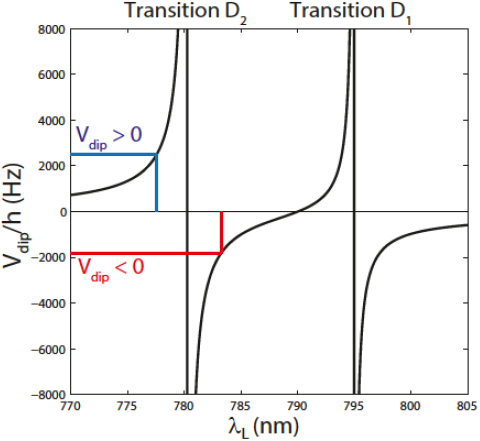
\includegraphics[scale=0.6]{Fig/BEC_manip/V_dip.png}
\caption{\textbf{Potentiel dipolaire en fonction de la longueur d'onde du laser.} La présence des deux transitions est remarquable par les deux divergences. Elles sont séparées par une zone de potentiel tantôt attractif, plus répulsif. Entre ces deux régimes se trouve une longueur d'onde \emph{magique} à environ \SI{790}{\nano\metre} pour laquelle le potentiel s'annule, quelque soit la puissance du laser.}
\label{fig:v_dip_magique}
\end{figure}

Naturellement, le rapprochement des transitions atomiques entraîne une augmentation du taux d'émission spontanée. Pour les désaccords considérés, il s'exprime
\begin{equation}
\Gamma_{\mathrm{sp}}=\frac{\pi c^2 I(\mathrm{r})}{2 \hb \omega_0^3} \left[ \left(\frac{\omega}{\omega_{D_1}} \right)^3 \left( \frac{\Gamma_{D_1}}{\omega-\omega_{D_1}} - \frac{\Gamma_{D_1}}{\omega+\omega_{D_1}} \right)^2 + 2\left( \frac{\omega}{\omega_0} \right)^3 \left( \frac{\Gamma}{\omega-\omega_0}-\frac{\Gamma}{\omega+\omega_0} \right)^2 \right]
\end{equation}
et l'ordre de grandeur du temps de vie associé est de l'ordre de quelques secondes.


Notons enfin qu'il est possible de se rapprocher encore plus de résonance et de devenir sensible à la structure hyperfine de la transition $D_2$ (dans ces conditions on peut négliger la contribution de la raie $D_1$). En revanche, le taux d'émission spontanée croît fortement et devient très contraignant.

\end{comment}
%%%%%%%%%%%%%%%%%%%%%%%%%%%%%%%%%%%


\paragraph*{Force de pression de radiation}
Le second terme s'appelle \emph{force de pression de radiation}. Il provient de la partie imaginaire de la polarisabilité atomique, qui caractérise l'absorption de photons par l'atome. Il s'agit donc d'une force inélastique qui résulte d'un grand nombre de cycles d'absorption de photons du faisceau laser et d'émission spontanée dans des directions aléatoires de l'espace \footnote{Pour réaliser de tels cycles, il est nécessaire d'avoir une transition cyclante, c'est à dire de disposer d'un état excité dont la désexcitation renvoie forcément sur l'état d'origine.}. L'impulsion totale cédée par émission spontanée s'annule donc, et en moyenne le transfert d'impulsion ne provient que de l'absorption de photons du faisceau laser. Ceci est illustré par le terme de droite de l'équation \ref{eq:forces_lumineuses}, faisant apparaître le gradient de la phase du laser $\nabla \phi (\mathbf{x})=\mathbf{k}$. 

On montre que cette force s'exprime \citep{cohen2012processus}:
\begin{equation}
\mathbf{F}_{\mathrm{PR}}=\hb \mathbf{k} \Gamma_{\mathrm{sp}} \text{ ,}
\end{equation}
avec $\Gamma_{\mathrm{sp}}$ le taux d'émission spontanée en présence du champ laser, et $\mathbf{k}$ le vecteur d'onde associé à l'onde laser. L'interprétation est directe: en moyenne, l'atome acquiert une impulsion $\hb \mathbf{k}$ à un taux $\Gamma_{\mathrm{sp}}$. Ce taux vaut:
\begin{equation}
\Gamma_{\mathrm{sp}}=\frac{\Gamma}{2} \frac{s}{1+s} \quad \text{avec} \quad s=\frac{I/I_{\mathrm{sat}}}{1+4\delta^2/\Gamma^2} \text{ ,}
\end{equation}
où l'intensité de saturation $I_{\mathrm{sat}}=\frac{\pi h c \Gamma}{3\lambda_0^3}=\SI{1.67}{\milli\watt\per\centi\metre^2}$ est une constante de l'atome de \isotope[87]{Rb}. La grandeur $s$ s'appelle le paramètre de saturation. Celui-ci dépend de l'intensité lumineuse incidente (et donc du nombre de photons incidents) ainsi que du désaccord du laser par rapport à la résonance atomique\footnote{L'expression \ref{eq:potentiel_dipolaire} n'est valable que dans un régime de faible saturation. L'utilisation de grands désaccords autorise l'utilisation de grosses puissances optiques tout en gardant $s\ll 1$. Dans ce régime, on peut estimer le taux d'émission spontanée par $\Gamma_{\mathrm{sp}}(\mathbf{x})=\frac{3 \pi c^2 I(\mathbf{x})}{2\hb \omega_0^3} \left( \frac{\omega}{\omega_0}\right)^3 \left( \frac{\Gamma}{\omega-\omega_0}-\frac{\Gamma}{\omega+\omega_0} \right)^2$.} $\delta = \omega-\omega_0$.  Le paramètre de saturation est maximal en $\delta=0$, c'est à dire lorsque le laser est à résonance. Dans le cas d'un laser très saturant $s \gg 1$, la force de pression de radiation s'écrit
\begin{equation}
\mathbf{F}_{\mathrm{PR}}=\frac{\hb \mathbf{k} \Gamma}{2} \text{ ,}
\end{equation}
où le facteur 2 indique que à forte saturation, un atome autant de chance d'être dans l'état excité que dans l'état fondamental. Enfin, mentionnons que pour un atome se déplaçant à une vitesse $\mathbf{v}$ dans le référentiel du laboratoire, le désaccord devient $\delta=\omega-\omega_0-\mathbf{k}.\mathbf{v}$ par effet Doppler. Nous reviendrons sur ce point lorsque nous décrirons les mécanismes du refroidissement laser.





\subsection{Couplage radio-fréquence} 
Les outils de manipulation des atomes présentés précédemment offrent la possibilité de créer des potentiels conservatifs (comme le potentiel dipolaire ou le potentiel magnétique) ou encore des forces dissipatives à l'aide la force de pression de radiation. De manière générale, certains de ces outils dépendent de l'état interne de l'atome\footnote{Le potentiel magnétique dépend bien évidemment de l'état interne, tandis que ce n'est pas de le cas du potentiel dipolaire dans la limite des grands désaccords.}, une dernière possibilité de manipulation des atomes consiste donc à contrôler leur état électronique. Un bon contrôle de ce degré de liberté permet donc d'augmenter l'efficacité des processus qui en dépendent (le chargement d'un piège magnétique par exemple), ainsi que de proposer des solutions technologiques originales. 

Comme présenté section \ref{sc:Rb87}, la séparation entre les états fondamentaux $\etatF{1}{}$ et $\etatF{2}{}$ correspond à une fréquence $\deltahf$ de l'ordre du \SI{}{\giga\hertz}, donc à une fréquence qui se trouve accessible électroniquement. Un couplage radio-fréquence entre ces états apparaît alors comme un formidable outil de contrôle de l'état interne des atomes, décrit par un système à deux niveaux dont le hamiltonien\footnote{Le terme de couplage \ref{eq:hamiltonien_rabi} est obtenu en appliquant l'approximation de l'onde tournante, c'est à dire que l'on néglige les termes en $\omega +\Delta_{\mathrm{hf}}$ devant les termes en $\omega - \Delta_{\mathrm{hf}}$ car on estime qu'ils évoluent rapidement, et donc qu'ils s'apparentent à leur valeur moyenne qui est nulle.} est donné dans la base $\etatF{1}{}, \etatF{2}{}$ par 
\begin{equation}
\hat{H}(t)=\frac{\hb}{2} \begin{pmatrix}
-\Delta_{\mathrm{hf}} & \Omega e^{i \omega t} \\
\Omega e^{-i\omega t} & \Delta_{\mathrm{hf}}
\end{pmatrix} \text{ ,}
\label{eq:hamiltonien_rabi}
\end{equation}
avec $\omega$ la fréquence de l'onde radio-fréquence, et $\Omega$ la pulsation de Rabi qui caractérise l'amplitude rayonnée sur les atomes.  En se plaçant dans le référentiel tournant, le hamiltonien du système devient
\begin{equation}
\hat{H}=\frac{\hb}{2} \begin{pmatrix}
\delta & \Omega \\
\Omega & -\delta
\end{pmatrix} \text{ ,}
\end{equation}
avec $\delta=\omega- \Delta_{\mathrm{hf}}$. En supposant que le système est dans l'état $\etatF{1}{}$ à $t=0$, la probabilité d'avoir l'atome dans l'état $\etatF{2}{}$ est donnée par la formule de Rabi \citep{basdevant2002mecanique}
\begin{equation}
\mathcal{P}_{\etatF{2}{}}(t)= \frac{\Omega^2}{\Omega^2+\delta^2} \sin^2{\left(\sqrt{\Omega^2+\delta^2} \frac{t}{2} \right) } \text{ .}
\label{eq:rabi_formule}
\end{equation}
Cette formule met en évidence un caractère résonant des transitions radio-fréquences:
\begin{itemize}
\item[\textendash] Dans le cas d'un grand désaccord $\delta \gg \Omega$, la probabilité de transition est très faible à n'importe quel instant.
\item[\textendash] À résonance $\delta=0$, la probabilité de transition peut atteindre 1, même pour un couplage très faible ($\Omega$ petit).
\end{itemize}
Ces caractéristiques sont illustrées figure \ref{fig:rabi}. En effet, l'enveloppe lorentzienne représentée figure \ref{fig:rabi}b montre les populations maximales transférées, faibles lorsque $\left| \delta \right| > \Omega$. On retrouve la condition de résonance à $\delta=0$, où l'efficacité de transfert est maximale.

\begin{figure}
\centering
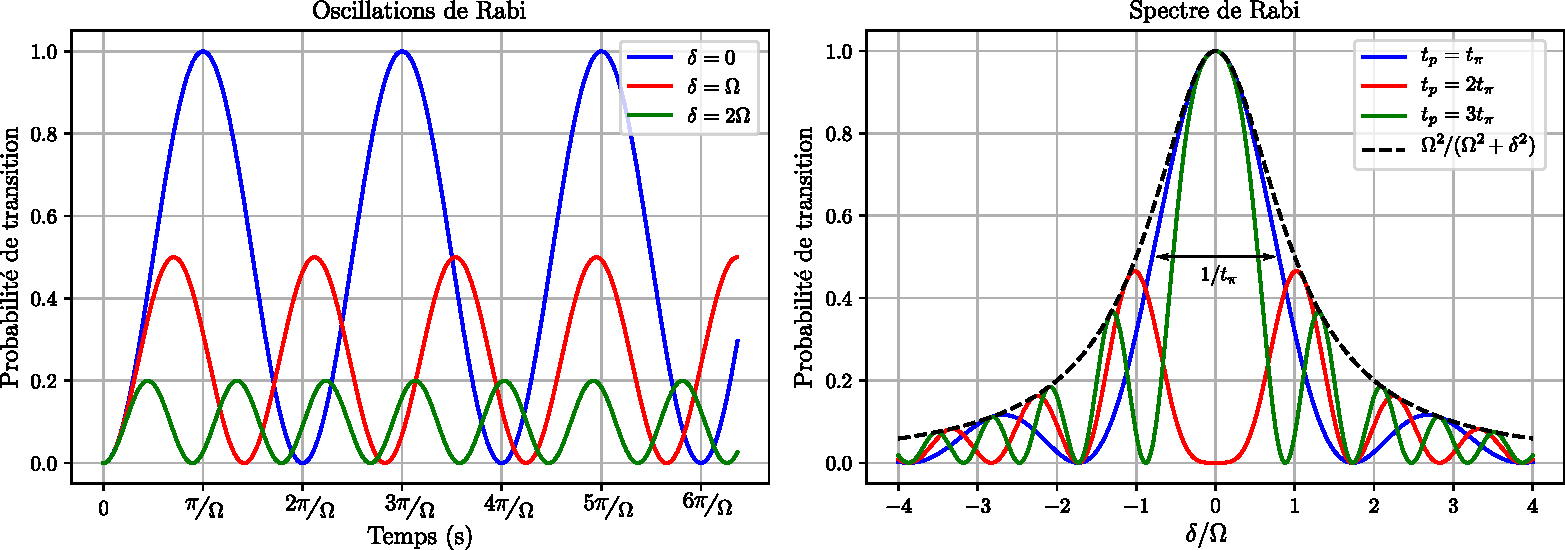
\includegraphics[width=\textwidth]{Fig/BEC_manip/rabi.pdf}
\caption{\textbf{a: Oscillations de Rabi tracées pour différents désaccords.} Les populations oscillent à la fréquence $\sqrt{\Omega^2+\delta^2}$ avec une amplitude qui dépend du désaccord. L'amplitude est maximale et atteint 1 lorsque l'onde radio-fréquence est à résonance, et la population maximale transférée décroît avec l'augmentation du désaccord. \textbf{b: Spectres de Rabi pour différentes durées d'application $t_p$.} Le transfert de population est le plus efficace à résonance ($\delta=0$), et l'utilisation d'un désaccord entraîne une diminution de l'efficacité de transfert. Les populations maximales transférées sont décrites par l'enveloppe lorentzienne de l'équation \ref{eq:rabi_formule}.}
\label{fig:rabi}
\end{figure}






\section{Description d'un cycle expérimental}
Dans la partie précédente, nous nous sommes familiarisés avec quelques outils couramment utilisés sur les expériences d'atomes ultra-froids pour piéger et manipuler les atomes. Dans cette nouvelle partie, nous nous pencherons sur l'implémentation de ces outils sur notre expérience afin d'obtenir un condensat de Bose-Einstein de \isotope[87]{Rb}. La présentation qui en est donnée ici se verra minimale, nous nous contenterons d'illustrer brièvement les différentes étapes de refroidissement qui mènent à la condensation. De nombreux détails pourront être trouvés dans les thèses des doctorants qui ont contribué à faire de cette expérience ce qu'elle est aujourd'hui: \citep{fauquembergue2004realisation}\citep{riou2006etude}\citep{bernard2010transport}\citep{jendrzejewski2012quantum}\citep{muller2015coherent}\citep{denechaud2018vers}\citep{mukhtar2019state}.

\subsection{Présentation générale du dispositif}
Comme toutes les expériences d'atomes ultra-froids, la manipulation des atomes se déroule sous ultra-vide afin de s'affranchir des conditions extérieures. En particulier, on évite ainsi les collisions avec des particules extérieures à température ambiante, ce qui chaufferait notre gaz et détruirait la cohérence d'un nuage condensé. Une vue d'ensemble de l'enceinte à vide est donnée figure \ref{fig:manip} qui montre aussi les pompes utilisées en continu pour maintenir le vide. Notre dispositif est composé d'un four chauffé à \SI{120}{\degreeCelsius} qui éjecte les atomes de rubidium, il s'agit de notre source d'atomes. Un doigt froid refroidi à \SI{-30}{\degreeCelsius} sert de diaphragme et permet de filtrer le jet d'atomes tout en adsorbant les atomes qui sont bloqués afin de pas polluer le vide. Un obturateur mécanique permet de couper le jet lorsqu'on ne souhaite pas accumuler des atomes en cours de cycle. Les atomes sont décélérés dans le ralentisseur Zeeman et capturés dans la première cellule où ils subissent les premières étapes de refroidissement. Ils sont ensuite transportés dans la seconde cellule où ils sont refroidis jusqu'à la condensation. C'est dans cette seconde cellule que se déroulent les expériences de science, on l'appelle alors \emph{Chambre de science}.

\begin{figure}
\centering
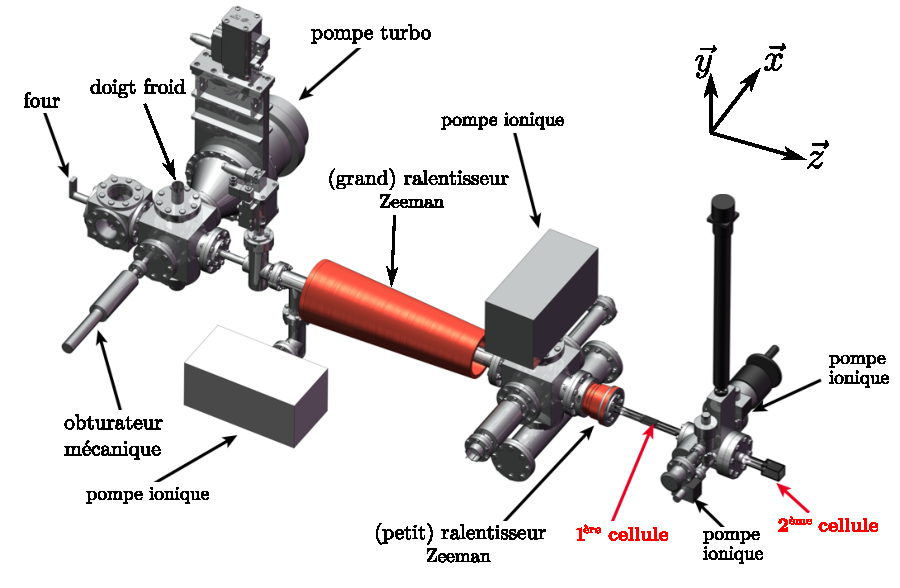
\includegraphics[width=\textwidth]{Fig/BEC_manip/manip.pdf}
\caption{\textbf{Vue d'ensemble du corps de l'expérience.} Les atomes se trouvent dans un montage sous ultra-vide, composé de deux chambres dans lesquelles les atomes sont manipulés.}
\label{fig:manip}
\end{figure}

\subsection{Première chambre}
C'est dans la première chambre que se déroulent les premières étapes de refroidissement du gaz de rubidium. Celles-ci sont dans un premier temps basées sur le refroidissement laser, puis dans un second temps sur un piégeage magnétique et l'évaporation forcée à l'aide d'un couteau radio-fréquence.

\paragraph*{Refroidissement laser}
Le principe du refroidissement laser repose sur la force de pression de radiation, présentée section \ref{sc:forces_lumineuses}. Plus particulièrement, le refroidissement laser consiste à dissiper de l'énergie cinétique à l'aide de cycles d'absorption et d'émission spontanée de photons. 

Considérons le cas d'un atome se déplaçant à vitesse $\mathbf{v}$ dans le référentiel du laboratoire soumis à une onde laser contrapropageante de pulsation $\omega$. Le désaccord du laser par rapport à la transition atomique s'exprime $\delta=\omega-\omega_0- \mathbf{k}. \mathbf{v}$, où le décalage Doppler $\mathbf{k}.\mathbf{v}<0$. Dans le référentiel de l'atome, la condition de résonance $\delta=0$ s'écrit $\omega_0=\omega-\mathbf{k}.\mathbf{v}$. L'atome va alors absorber un photon laser d'énergie $\hb \omega$ et en émettre un d'énergie supérieure $\hb \omega_0$ par émission spontanée. Il y a donc eu un transfert d'énergie entre l'énergie cinétique et le désaccord. La répétition de tels cycles permet ainsi de transférer beaucoup d'énergie cinétique de l'atome vers le désaccord entre photons absorbés et photons rayonnés.

La possibilité de répéter ces cycles d'absorption de photons et d'émission spontanée repose sur l'existence d'une transition cyclante entre les états hyperfins $\etatF{2}{}$ et $\etat{F'=3}$. La désexcitation de $\etat{F'=3}$ renvoie forcément l'atome dans l'état $\etatF{2}{}$ car les règles de sélection imposent $F'-F= \lbrace 0, \pm 1 \rbrace$.
En revanche, on peut accidentellement envoyer des atomes dans l'état excité $\etat{F'=2}$ car la séparation avec l'état ciblé $\etat{F'=3}$ n'est que de \SI{266}{\mega\hertz}. Statistiquement, un atome visite cet état tous les 50 cycles environ, et sa désexcitation peut faire tomber les atomes dans l'état $\etatF{1}{}$. Cet état étant un état noir, pour conserver les atomes, on doit alors utiliser un second laser appelé \emph{repompeur} qui permet de recycler les atomes perdus vers la transition cyclante\footnote{À titre d'illustration, le temps de vie du piège magnéto-optique a été mesuré à une dizaine de secondes. Sans le faisceau repompeur, les atomes tombent dans l'état noir $\etatF{1}{}$ en quelques micro-secondes seulement.}. Il est accordé sur la transition $\etatF{1}{} \rightarrow \etat{F'=2}$.

Notre dispositif laser se compose alors d'un laser principal de refroidissement accordé sur la transition $\etatF{2}{} \rightarrow \etat{F'=3}$. Il est secondé d'un second laser \emph{repompeur} accordé sur la transition $\etatF{1}{} \rightarrow \etat{F'=2}$. Enfin un dernier laser sert de référence de fréquence pour les deux précédents en étant asservi par absorption saturée. Une représentation schématique de l'ensemble de ces lasers et de leur amplification peut être trouvée figure \ref{fig:table_optique}.

\begin{figure}
\centering
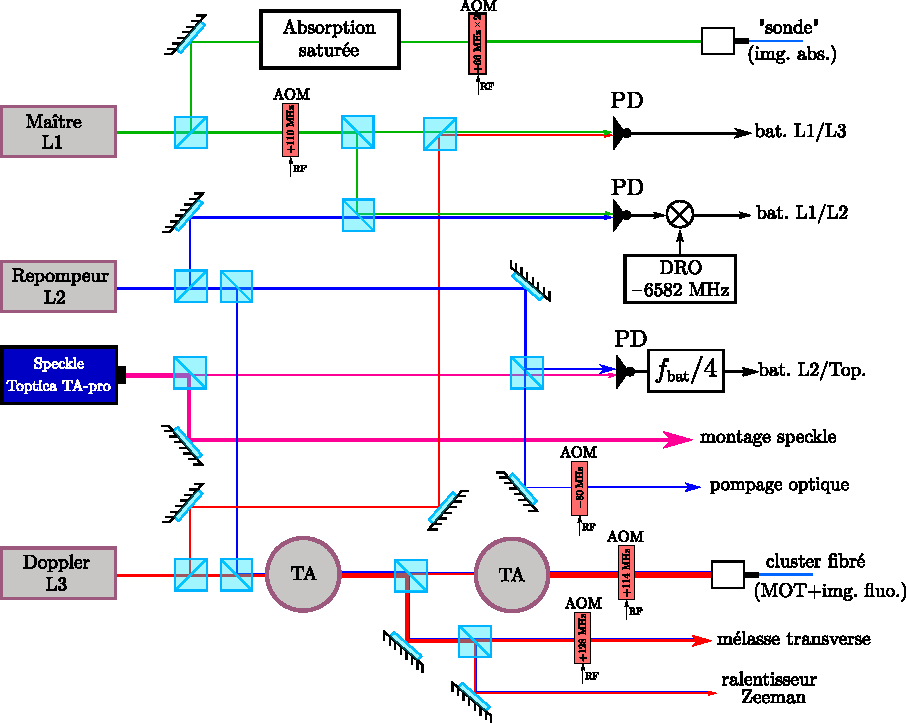
\includegraphics[width=0.8\textwidth]{Fig/BEC_manip/table_optique2.pdf}
\caption{\textbf{Représentation schématique de notre montage laser.} Le laser maître \emph{L1} sert de référence de fréquence en étant asservi par absorption saturée. Le laser de refroidissement Doppler \emph{L3} est asservi par battements avec \emph{L1}. Le laser repompeur \emph{L2} est lui aussi asservi par battements avec \emph{L2} grâce à l'utilisation d'électronique rapide. Notons enfin que les faisceaux de \emph{L2} et \emph{L3} sont mélangés avant amplification (TA). Les faisceaux arrivant sur les atomes comporteront alors les fréquences provenant de ces deux lasers. Un obturateur mécanique (non représenté) permet de couper le faisceau de \emph{L2} allant vers les amplificateurs.}
\label{fig:table_optique}
\end{figure}

\paragraph*{Le ralentisseur Zeeman}
La première étape consiste à ralentir suffisamment le jet d'atomes pour pouvoir les capturer dans un premier piège. Un laser désaccordé vers le rouge par rapport à la transition cyclante $\etatF{2}{} \rightarrow\etat{F'=3}$ permet de réaliser une décélération des atomes à l'aide de cycles d'absorption et d'émission spontanée de photons. Cependant, le ralentissement des atomes désaccorde le faisceau laser de la résonance atomique par effet Doppler. Pour palier à ce problème, on applique un champ magnétique pour satisfaire localement la condition de résonance par effet Zeeman\footnote{D'autres solutions furent envisagées lors des premiers développement des expériences d'atomes froids. Parmi celles-ci, mentionnons les faisceaux lasers \emph{chirpés} \citep{ertmer1985laser} et les lasers spectralement larges \citep{zhu1991continuous}.}. Ce champ est appliqué à l'aide d'une bobine comportant un nombre de tours par unité de longueur variable, représentée figure \ref{fig:manip} entre le four et la première chambre.
Ainsi, on est capable de réduire la vitesse des atomes de \SI{100}{\metre\per\second} à environ \SI{20}{\metre\per\second} sur une distance de seulement \SI{1}{\metre}.

\paragraph*{Le piège magnéto-optique}
Une fois les atomes suffisamment ralentis, ils sont capturés dans le piège magnéto-optique (abrégé en \emph{MOT} pour l'anglais \textit{Magneto-Optical Trap}). Celui-ci est composé de trois paires de faisceaux contra-propageants désaccordés vers le rouge d'environ $\delta=\SI{-16}{\mega\hertz}$, de polarisations opposées $\sigma^+$ et $\sigma^-$. Chacun de ces faisceaux possède une puissance d'environ \SI{12}{\milli\watt}.
De plus, deux bobines en configuration anti-Helmholtz permettent de générer un champ quadrupolaire, donc un gradient magnétique dans les trois directions de l'espace, afin de créer une force de rappel.
On charge environ \num{2e9} atomes en moins d'une seconde grâce à la mélasse transverse qui permet de collimater le jet d'atomes et donc d'améliorer le flux. 
Une fois le chargement saturé, on coupe le champ magnétique pendant quelques millisecondes afin de réduite fortement la température: c'est l'étape de mélasse optique qui permet de descendre la température à environ \SI{50}{\micro\kelvin}. 

\begin{figure}
\centering
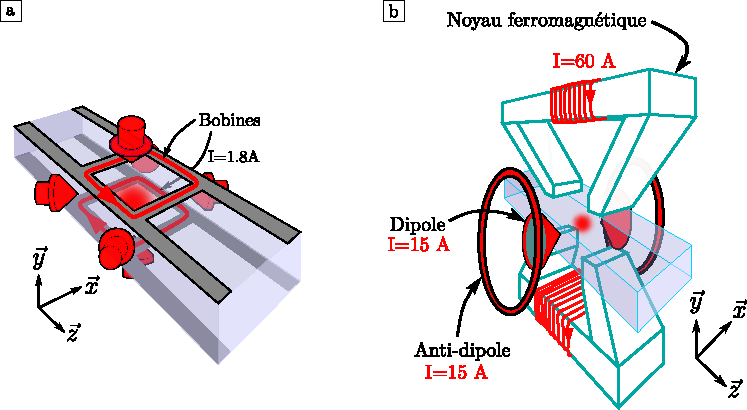
\includegraphics[width=\textwidth]{Fig/BEC_manip/MOT_magtrap.pdf}
\caption{\textbf{a: Éléments du piège magnéto-optique.} Il est réalisé à l'aide de trois paires de faisceaux contra-propageants et de deux bobines formant un champ quadrupolaire. Ces bobines sont faites à partir de circuits imprimés posés sur la cellule. \textbf{b: Géométrie du piège magnétique.} Un champ quadrupolaire intense est créé selon les directions $\vec{y}$ et $\vec{z}$ par un électroaimant. Un champ de biais est généré par deux paires de bobines suivant la direction $\vec{x}$. Ce champ possède une courbure longitudinale et est responsable du confinement suivant cette direction. }
\label{fig:MOT_magtrap}
\end{figure}

\paragraph*{Piège magnétique et évaporation radio-fréquence}
À l'issue de l'étape de mélasse, les atomes sont chargés dans un piège magnétique qui va permettre de se rapprocher considérablement du seuil de condensation. Afin d'augmenter le nombre d'atomes piégeables magnétiquement, il est nécessaire de manipuler l'état interne des atomes. On procède ainsi à une étape de dépompage en éteignant le faisceau de repompage et en accordant le faisceau de refroidissement sur la transition $\etatF{2}{} \rightarrow\etat{F'=2}$: en moins d'une milliseconde, les atomes se trouvent dans l'état $\etatF{1}{}$, dont seul le sous-état Zeeman $\etatF{1}{-1}$ peut être piégé\footnote{Il est le seul des trois sous-états Zeeman de $\etatF{1}{}$ à avoir le produit $g_{\mathrm{F}} \mf > 0$, c'est à dire qu'il s'agit d'un état \emph{Low Field Seeker}, qui est attiré par les zones de faible champ magnétique. En effet, c'est à l'aide d'un minimum de champ magnétique que l'on réalise ce piège, le théorème de Wing interdisant les maximas de champ magnétique. }\footnote{Des huit sous-états Zeeman fondamentaux, il s'agit de celui ayant la plus grande probabilité d'occupation tout en étant piégeable, justifiant son choix. }. Afin de maximiser la population de ce sous-état, on allume un faisceau de pompage optique accordé sur la transition $\etatF{1}{} \rightarrow \etat{F'=1}$ et polarisé $\sigma^-$ pendant \SI{40}{\micro\second}. En parallèle, on allume le champ du \emph{dipôle} afin de définir un axe de quantification.

Le piège magnétique que l'on utilise est un piège de type \emph{Ioffe-Pritchard}. Il est composé essentiellement de deux éléments:
\begin{itemize}
\item[\textendash] Un champ de biais orienté dans la direction $\vec{x}$, généré par une paire de bobines (\emph{dipôle}) de configuration légèrement plus éloignée que celle de Helmholtz: on a ainsi une courbure positive dans la direction longitudinale au centre des bobines. Une seconde paire de bobines (\emph{anti-dipôle}) permet d'abaisser le champ constant au centre du piège sans changer significativement sa courbure. Cet abaissement du biais magnétique se traduit par une compression du nuage \citep{fauquembergue2004realisation}.
\item[\textendash] Un champ quadrupolaire dans le plan $(\vec{y},\vec{z})$ généré par un électroaimant ferromagnétique épais (\emph{quadrupôle}) comportant deux entrefers et deux bobines excitatrices dans deux sens opposés. L'épaisseur importante du matériau magnétique minimise l'effet de l'électroaimant dans la direction $\vec{x}$.
\end{itemize}
Le confinement dans la direction $\vec{x}$ est donc réalisée par le champ de \emph{dipôle}\footnote{Notons que la présence du champ de dipôle permet aussi de s'affranchir des pertes par transition Majorana, le champ ne s'annulant à aucun endroit de l'espace.}, tandis que le confinement dans les directions $\vec{y}$ et $\vec{z}$ est fait par le \emph{quadrupôle}. 
On obtient ainsi un nuage piégé magnétiquement comportant environ \num{1e9} atomes tous dans le même sous-état zeeman à une température de $\sim \SI{300}{\micro\kelvin}$.

Une fois le nuage thermalisé, on procède à une étape de refroidissement évaporatif grâce à la méthode de \emph{couteau radio-fréquence}. Une étude détaillée du refroidissement évaporatif est proposée section \ref{sc:evap_optique}, mais on peut en résumer le principe, illustré figure \ref{fig:evapRF}, de la manière suivante:
\begin{itemize}
\item[\textendash]On tronque le piège de telle sorte que quelques atomes très énergétiques (la queue de la distribution de vitesses de Maxwell-Boltzmann) puissent s'en échapper, chaque atome emportant une énergie supérieure à l'énergie moyenne par atome.
\item[\textendash]Les collisions entre les particules étant restées dans le piège permettent au système de thermaliser. Ce nouvel état d'équilibre thermique est caractérisé par une température plus basse.
\end{itemize}

La troncature du piège se fait à l'aide d'une onde radio-fréquence rayonnée par les bobines MOT. Celle-ci induit une transition de l'état piégé $\etatF{1}{-1}$ à l'état non piégé $\etatF{1}{0}$ lorsque la condition de résonance $\hb \omega_{\mathrm{RF}} = \mf g_{\mathrm{F}} \mub B(\mathbf{x})$ est vérifiée. En abaissant progressivement la fréquence rayonnée pendant une dizaine de secondes, on obtient finalement un nuage d'environ \num{70e6} atomes à une température de \SI{10}{\micro\kelvin}.

\begin{figure}
\centering
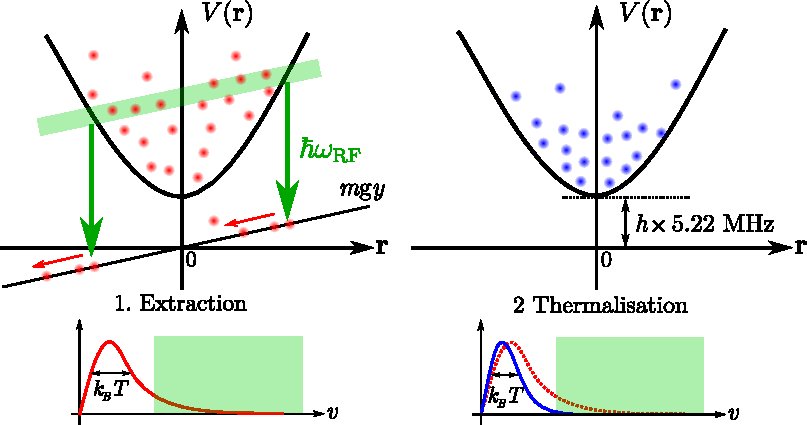
\includegraphics[width=0.9\textwidth]{Fig/BEC_manip/evapRF.pdf}
\caption{\textbf{Principe de l'évaporation radio-fréquence.} L'application d'une radio-fréquence permet de tronquer le piège magnétique, et d'éliminer les atomes les plus énergétiques. L'énergie moyenne par particule étant plus basse, la température s'en retrouve abaissée après thermalisation.}
\label{fig:evapRF}
\end{figure}


\subsection{Chambre de science}
\label{sc:chambre_science}
Après ces premières étapes de refroidissement, les atomes sont transportés dans une seconde cellule où l'on procède à une évaporation tout-optique pour franchir le seuil de condensation. La raison d'être de cette seconde cellule est de profiter d'un maximum d'accès optiques tout en s'affranchissant de l'environnement magnétique de la première chambre, en particulier celui du ferromagnétique.
Nous nous contenterons ici de présenter les grandes lignes des éléments de cette seconde chambre, de nombreux détails pourront être trouvés dans la thèse d'Alain Bernard \citep{bernard2010transport}, dans la thèse de Fred Jendrzejewski \citep{jendrzejewski2012quantum} et de Kilian Muller \citep{muller2015coherent}. De plus, certains de ces éléments ont été modifiés au cours de ma thèse et une étude plus approfondie en sera présentée dans le chapitre \ref{ch:new_exp}.

\paragraph*{Transport dans une pince optique et piège dipolaire croisé}
Après évaporation radio-fréquence, on transfert le nuage dans une pince optique. Il s'agit d'un piège dipolaire créé par focalisation sur les atomes d'un faisceau laser de longueur d'onde $\lambda=\SI{1070}{\nano\metre}$ et de puissance estimée d'environ \SI{1.5}{\watt}. Dans le plan focal, ce faisceau a une taille $\mathrm{w}_{\mathrm{0}}=\SI{28}{\micro\metre}$ et la distance de Rayleigh vaut donc $z_{\mathrm{R}}= \pi \mathrm{w}_{\mathrm{0}}^2 / \lambda=\SI{2.3}{\milli\metre}$. On obtient ainsi \num{10e6} atomes à une température de \SI{10}{\micro\kelvin} aux alentours du foyer de la pince\footnote{Ce faible taux de transfert entre le piège magnétique et la pince provient du mauvais recouvrement spatial entre ces deux pièges. La pince est très allongée suivant la direction $\vec{z}$, tandis que le piège magnétique est étendu suivant la direction $\vec{x}$. Cette géométrie est un héritage des débuts de cette expérience, originellement utilisée pour étudier le laser à atomes.}.

Le transport dans la seconde chambre se fait à l'aide d'une platine de translation montée sur coussin d'air \emph{Aerotech ABL80040}. Les optiques de focalisation de la pince se trouvant sur cette platine, on déplace ainsi les atomes de \SI{40}{\centi\metre} en moins de \SI{2}{\second}, comme illustré figure \ref{fig:piege_optique}. On estime l'efficacité de transfert à 75\%, mesurée en effectuant un aller-retour pour retourner dans la première chambre.

\begin{figure}
\centering
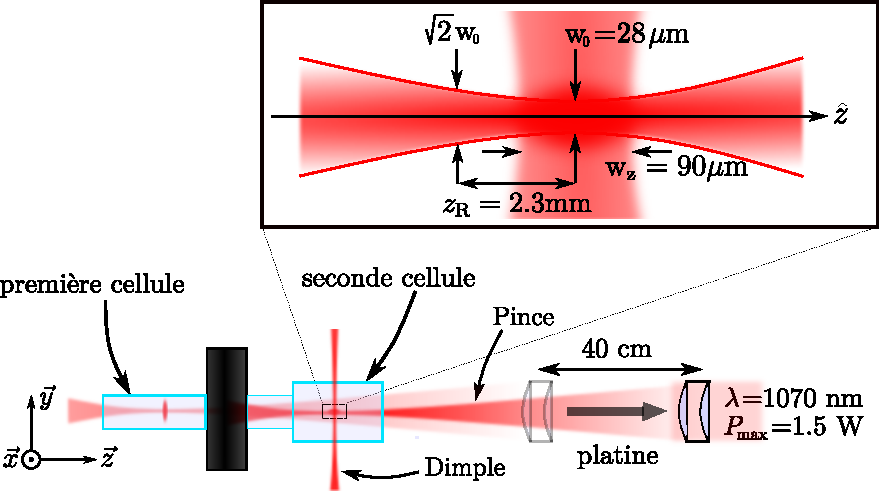
\includegraphics[width=0.9\textwidth]{Fig/BEC_manip/piege_optique2.pdf}
\caption{\textbf{Illustration du transport et du piège optique.} Les atomes sont capturés autour du foyer de la pince dans la première chambre, et le point de focalisation est déplacé de \SI{40}{\centi\metre} à l'aide d'une platine de translation. Une fois le transport terminé, on allume un second faisceau de piégeage vertical (\emph{dimple}).}
\label{fig:piege_optique}
\end{figure}

Une fois les atomes arrivés dans la seconde chambre, un second faisceau de piégeage dipolaire de longueur d'onde \SI{1070}{\nano\metre} et de puissance \SI{7}{\watt} est allumé afin de comprimer le nuage suivant la direction $\vec{z}$ qui correspond à la direction longitudinale de la pince. Ce faisceau \emph{Dimple} est de forme elliptique, de tailles $\SI{180}{\micro\metre} \times \SI{90}{\micro\metre}$ dans les directions $\vec{x}$ et $\vec{z}$ respectivement. Étant donnée sa grande longueur de Rayleigh (de l'ordre du centimètre), on suppose que le piégeage vertical induit est négligeable devant toutes les autres sources de piégeage. Ainsi, dans le piège dipolaire croisé, le confinement suivant les directions $\vec{x}$ et $\vec{y}$ est fait par la pince, tandis que le confinement suivant la direction $\vec{z}$ est fait par le faisceau vertical\footnote{La forme allongée du dimple dans la direction $\vec{x}$ fait que le piégeage dans cette direction est très faible comparé à celui de la pince. De plus, cela rend le piège optique tolérant face à un léger défaut d'alignement.}, comme illustré figure \ref{fig:piege_optique}. À ce stade, on estime disposer de \num{3e6} atomes à une température de \SI{10}{\micro\kelvin}.

Enfin, une dernière étape d'évaporation est requise pour franchir le seuil de condensation. Succinctement, celle-ci consiste à diminuer la puissance des lasers afin de diminuer la profondeur des potentiels de piégeage de telle sorte que les atomes les plus énergétiques puissent s'échapper. Cette étape sera étudiée plus en détails dans la partie \ref{sc:evap_optique}.



\paragraph*{Lévitation magnétique}
Une contrainte liée à l'étude la localisation d'Anderson réside dans les grands temps de propagation dans le désordre requis. Dans l'expérience visant à observer la localisation d'Anderson à trois dimensions, plusieurs secondes d'évolution dans le désordre ont été nécessaires \citep{jendrzejewski2012three}, ce qui n'est pas possible en présence de la gravité. En conséquence notre expérience dispose d'une lévitation magnétique permettant de s'affranchir de la gravité et donc de multiplier nos possibilités expérimentales. Celle-ci a été mise en place durant la thèse d'Alain Bernard et de nombreux détails concernant ce système et ses performances se trouvent dans son manuscrit. Cependant, la lévitation magnétique a fait l'objet d'une attention particulière durant ma thèse, aussi une étude approfondie en sera donnée dans la partie \ref{sc:levitation}. Donnons en tout de même quelques caractéristiques.

Le principe de la lévitation magnétique est de compenser la force de pesanteur à l'aide d'un gradient magnétique. Pour l'état $\etatF{1}{-1}$ qui est \emph{Low Field Seeker}, il s'agit d'un gradient de \SI{30}{\gauss\per\centi\metre}. Cependant, le théorème de Wing impose une valeur minimale aux fréquences de piégeage dues à la conservation du flux magnétique:
\begin{equation}
\sum_{i=x,y,z} \omega_i^2 \geq \left| \frac{mg^2}{2 \mf g_{\mathrm{f}} \mub \Bzero}\right| \text{ ,}
\label{eq:theoreme_wing}
\end{equation} 
avec $g$ l'accélération de la pesanteur et $B_0$ la norme du champ magnétique à la position des atomes. Une stratégie de réduction de ces fréquences de piégeage (les $\omega_i$ sont positifs pour l'état $\etatF{1}{-1}$) consiste à augmenter fortement le champ $\Bzero$, on utilise alors des bobines pour créer un tel champ, qui peut monter jusqu'à \SI{2000}{\gauss}, entraînant des fréquences de piégeage de l'ordre de $\omega_i /2 \pi \sim \SI{0.2}{\hertz}$. Une version simpliste du design de notre lévitation est donnée figure \ref{fig:levitation_simple}.

Une autre stratégie couramment utilisée par l'équipe est de se placer dans l'état $\etatF{2}{-2}$ qui est \textit{High Field Seeker}, il sera donc expulsé de la lévitation par les courbures résiduelles. Il s'agit pour nous d'un avantage puisque cela favorise le processus d'évaporation, de plus on ne pourra pas attribuer à la lévitation un éventuel arrêt de l'expansion du nuage dans l'étude de la localisation d'Anderson. Pour atteindre cet état, on applique une transition radio-fréquence dans le piège optique croisé avant évaporation.

\begin{figure}
\centering
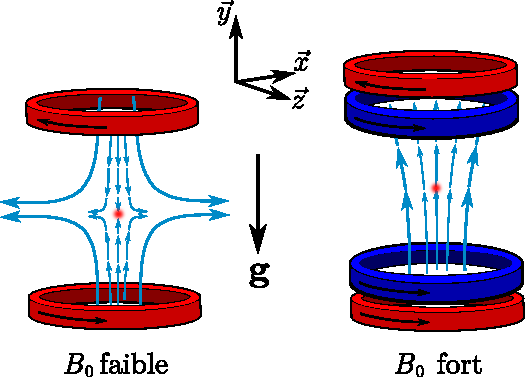
\includegraphics[scale=1]{Fig/BEC_manip/levitation_simple.pdf}
\caption{\textbf{Design simplifié de la lévitation magnétique}. Un gradient magnétique est appliqué aux atomes grâce à une paire de bobines parcourues par des courants opposés. La conservation du flux magnétique entraîne des gradients dans les autres directions de l'espace. L'application d'un fort champ de biais créé par d'autres bobines permet de minimiser l'impact de ces gradients et de diminuer les fréquences de piégeage (ou d'anti-piégeage) associées.}
\label{fig:levitation_simple}
\end{figure}

Pour finir, citons un dernier avantage offert par la lévitation magnétique: la compensation de la gravité n'entraîne pas d'effet \emph{SAG}, c'est à dire que la gravité ne vient pas "pencher" le potentiel de notre piège optique. Nous avons donc la possibilité de pousser l'évaporation optique jusque dans un domaine où la gravité aurait normalement dû tirer les atomes en dehors du piège, nous pouvons ainsi évaporer beaucoup plus loin et atteindre des températures extrêmement basses.



\paragraph*{Refroidir encore plus}
L'assimilation d'un condensat de Bose-Einstein à une onde de matière monochromatique $\etat{k=0}$ nécessite de pouvoir négliger la largeur de distribution de vitesses $\Delta k$, et implique donc d'obtenir des nuages extrêmement froids. Bien que la lévitation magnétique nous permette d'obtenir des températures particulièrement basses, le refroidissement peut être poussé encore plus loin. 

Une première technique consiste en une décompression du nuage à l'aide de l'ouverture adiabatique du piège. Cette décompression se traduit par une diminution des fréquences de piégeage, que l'on obtient en changeant la taille des faisceaux de piégeage. En pratique, il nous suffit de reculer le plan de focalisation de la pince de \SI{4.5}{\milli\metre} en une seconde à l'aide de la platine de translation comme illustré figure \ref{fig:adia_opening_and_delta_kick}a. La température obtenue est alors donnée par le théorème d'équipartition de l'énergie:
\begin{equation}
T'=\frac{\omega_{\mathrm{r}}'}{\omega_{\mathrm{r}}}T < T \text{ ,}
\end{equation}
avec $\omega_{\mathrm{r}}$ la fréquence de piégeage de la pince dans la direction radiale. L'abaissement de la température est donc obtenu par diminution de la densité du nuage, c'est à dire par dilution. Cette étape se déroule en même temps que l'évaporation optique.

À la fin du cycle d'évaporation et d'ouverture adiabatique, il reste environ \num{2e5} atomes dont environ 50\% forment un condensat de Bose-Einstein. Le potentiel chimique de la partie condensée est estimée à $\mu/h=\SI{40}{\hertz}$, et la température de la fraction thermique est d'environ \SI{5}{\nano\kelvin}. 

\begin{figure}
\centering
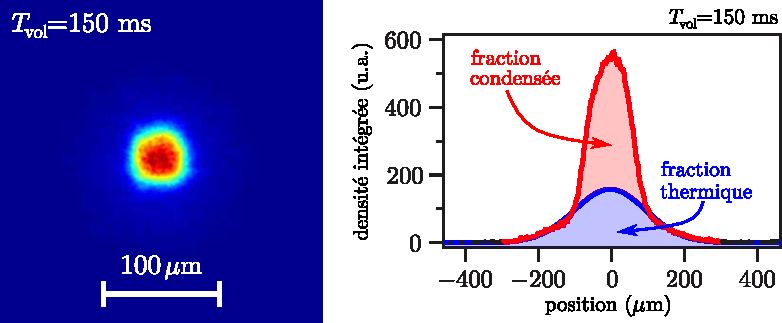
\includegraphics[width=0.9\textwidth]{Fig/BEC_manip/BEC_double_struct.pdf}
\caption{\textbf{Image expérimentale d'un condensat de Bose-Einstein}. Cette image correspond à celle d'un condensat après expansion pendant un temps de vol de \SI{150}{\milli\second}. L'image de droite correspond au profil de la densité intégrée suivant une direction, et montre la double structure témoignant d'une partie condensée. La partie condensée a un profil parabolique (en rouge), tandis que la partie thermique est de forme gaussienne (en bleu).}
\label{fig:BEC_double_struct}
\end{figure}

Après l'extinction du piège, l'énergie d'interaction du nuage est convertie en énergie cinétique, le nuage s'étend alors librement grâce à la lévitation. L'évolution de la taille du nuage donne alors accès à la distribution de vitesse, en particulier à sa dispersion $\Delta k \simeq \SI{0.5}{\per\micro\metre}$. Une dernière technique reposant aussi sur le principe de la dilution permet de réduire davantage cette dispersion. Cette technique dite de \emph{refroidissement par delta-kick} consiste à transférer l'énergie d'interaction en énergie cinétique en éteignant le piège, puis à figer le mouvement des atomes en appliquant un potentiel harmonique pendant un bref instant. L'énergie cinétique est alors transformée en énergie potentielle, disparaissant à l'extinction du piège. Une illustration de ce procédé est donnée figure \ref{fig:adia_opening_and_delta_kick}b.

Une approche classique permet de justifier cela. En supposant que l'expansion des atomes est balistique, la position des atomes après un temps d'expansion $t_{\mathrm{exp}}$ suffisamment grand est donnée par leur vitesse initiale:
\begin{equation}
\mathbf{x}(t_{\mathrm{exp}})=\mathbf{v} t_{\mathrm{exp}} \text{ .}
\end{equation}
Appliquons un kick de potentiel harmonique pendant un temps $\Delta t$. La vitesse des atomes à la fin de ce kick est donnée par
\begin{equation}
\dot{\mathbf{x}}(\Delta t) = -\mathbf{x} \omega \sin{(\omega \Delta t)}+ \mathbf{v} \cos{(\omega \Delta t)} \text{ ,}
\end{equation}
avec $\omega$ la fréquence du piège.
On peut trouver $\Delta t$ tel que $\dot{\mathbf{x}}_i=0$:
\begin{equation}
\Delta t= \frac{1}{\omega} \arctan{\left(\frac{1}{t_{\mathrm{exp}} \omega} \right)} \text{ .}
\end{equation}
On remarque que $\Delta t$ ne dépend pas de la vitesse initiale des atomes: on peut donc geler l'ensemble du nuage en appliquant un potentiel harmonique pendant la bonne durée de kick\footnote{Une approche équivalente consiste à dire que la force de rappel est proportionnelle à la distance parcourue par les atomes, qui est proportionnelle à la vitesse initiale. L'instant où les vitesses s'annulent ne dépend donc pas de la vitesse initiale des atomes.}. 
La mise en œuvre expérimentale de cette technique est détaillée dans le manuscrit de thèse de Kilian Muller \citep{muller2015coherent} et témoigne de résultats impressionnants: la dispersion en vitesse s'est abaissée à $\Delta k \simeq \SI{0.15}{\per\micro\metre}$. La température effective associée est alors de $T\sim \SI{150}{\pico\kelvin}$, et en tenant compte de la taille du nuage de l'ordre de $\Delta x \sim \SI{30}{\micro\metre}$, on s'approche à un ordre de grandeur de la limite de Heisenberg $\Delta x \hb \Delta k \simeq 10 \hb /2$.

\begin{figure}
\centering
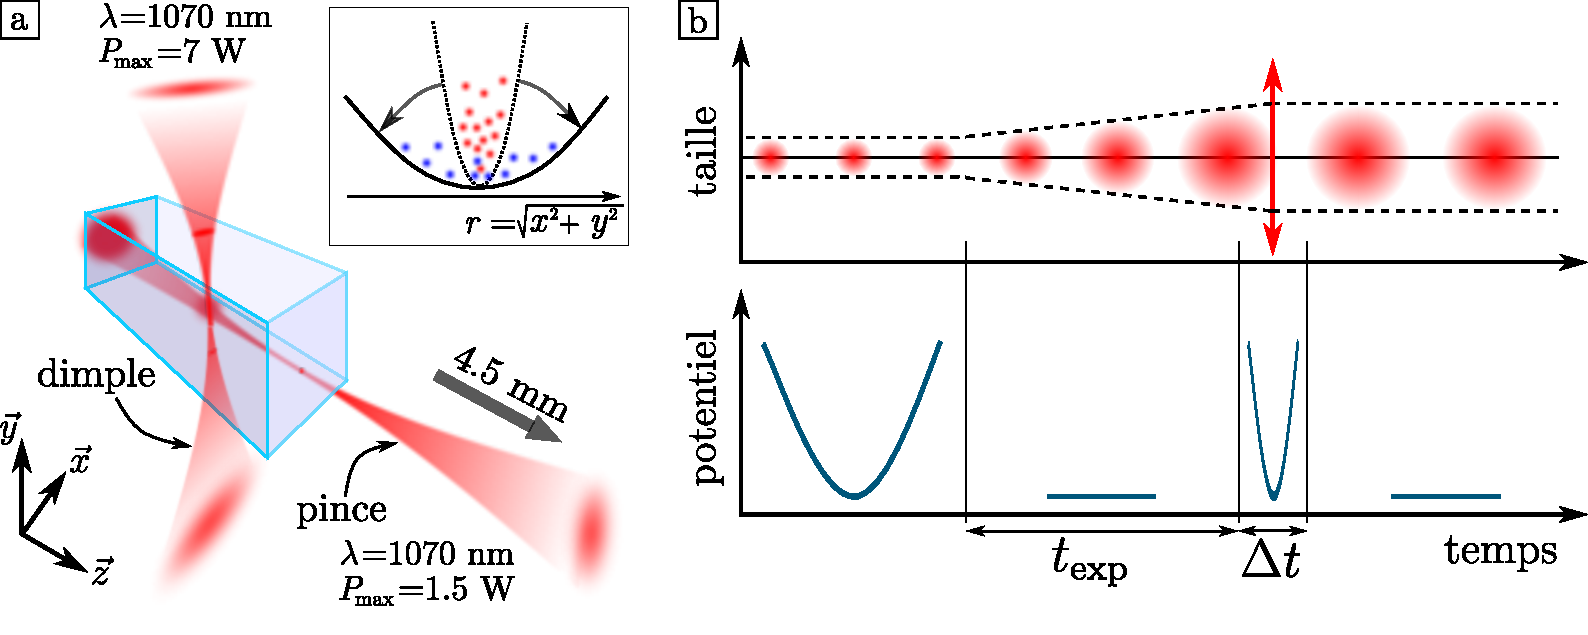
\includegraphics[width=\textwidth]{Fig/BEC_manip/adia_opening_and_delta_kick2.pdf}
\caption{\textbf{a: Principe de l'ouverture adiabatique.} Le déplacement du point de focalisation de la pince permet d'augmenter la taille du faisceau au niveau des atomes. La fréquence de piégeage en est alors diminuée, et on abaisse alors la température par dilution. \textbf{b: Illustration du refroidissement par \emph{delta-kick}.} L'extinction du piège entraîne l'étalement du nuage, et le transfert de l'énergie d'interaction en énergie cinétique. On peut ensuite \textit{focaliser} les atomes à l'aide d'un \textit{kick} de potentiel, en transformant l'énergie cinétique en énergie potentielle, supprimée à l'extinction du piège.}
\label{fig:adia_opening_and_delta_kick}
\end{figure}















\subsection{Imagerie}
\label{sc:imagerie}
À la fin de la majorité de nos cycles expérimentaux, nous souhaitons obtenir des informations à propos de notre gaz d'atomes. Une grande partie de ces informations peut être extraite d'une image du nuage après extinction du piège, image que l'on obtient à l'aide d'une caméra et l'utilisation de lasers à résonance avec les atomes \footnote{L'utilisation de lasers à résonance conduit inévitablement à la destruction du nuage sur notre expérience. Il est donc nécessaire de répéter l'ensemble du cycle expérimental pour obtenir une seconde image des atomes.}. L'utilisation d'un retard (appelé \emph{temps de vol} et abrégé en \emph{TOF} pour l'anglais \textit{Time Of Flight}) entre l'extinction du piège et la prise de l'image est extrêmement courant fournit de précieux renseignements.

\paragraph*{Dispositif d'imagerie}
L'expérience est équipée de trois caméras \textit{EMCCD C9102} de chez \textit{Hamamatsu}, chacune comportant une matrice de $1000 \times 1000$ pixels de taille $\SI{8}{\micro\metre} \times \SI{8}{\micro\metre}$. Ces trois caméras sont contrôlées via l'outil d'acquisition d'images de MATLAB, qui permet aussi de récupérer et traiter les images obtenues. L'acquisition des images est déclenchée de manière externe par le séquenceur.\\
Une première caméra acquiert des images des atomes dans la première chambre selon l'axe horizontal $\vec{x}$ avec un grandissement de 1, la zone imageable est donc de $\SI{8}{\milli\metre} \times \SI{8}{\milli\metre}$. Il est possible d'utiliser cette caméra pour de l'imagerie par absorption (représentée figure \ref{fig:img_mot}) aussi que pour de l'imagerie par fluoresence grâce à un montage 4$f$. Néanmoins, l'observation selon une direction induit forcément une intégration de la densité suivant cette direction: on ne peut mesurer qu'une densité intégrée
\begin{equation}
n_{\mathrm{2D}}(y,z) =\int{\mathrm{d}x \: n(x,y,z)} \text{ ,}
\end{equation}
avec $n$ la densité à trois dimensions.\\
Les deux autres caméras sont positionnées autour de la chambre de science selon l'axe horizontal $\vec{x}$ et vertical $\vec{y}$. Toutes deux voient le nuage au travers d'un système optique de grandissement 3\footnote{Ce grandissement a été mesuré on observant la chute libre du nuage en l'absence de la lévitation.}, conduisant à une résolution de \SI{2.71}{\micro\metre} pour une zone imageable de $\SI{2.71}{\milli\metre} \times \SI{2.71}{\milli\metre}$. Seule de l'imagerie par fluorescence est utilisable dans cette chambre, en revanche il est possible d'utiliser ces deux caméras simultanément pour obtenir les densités intégrés suivant deux directions $n_{\mathrm{2D}}(y,z)$ et $n_{\mathrm{2D}}(x,y)$ pour le même nuage.

\paragraph*{Imagerie par absorption}
Le principe de l'imagerie par absorption repose sur la loi de Beer-Lambert. En effet, lorsque qu'un faisceau laser traverse un milieu, son absorption dépend directement de la densité du milieu en particules absorbantes (la densité atomique dans notre cas). Pour sonder cette densité atomique, on envoie donc un faisceau laser à résonance directement sur les atomes et la caméra comme illustré figure \ref{fig:img_mot}. 
\begin{figure}
\centering
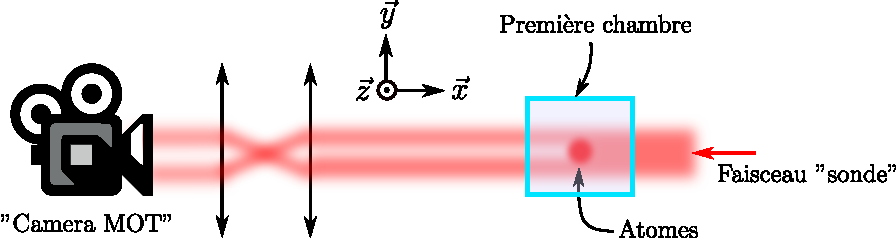
\includegraphics[width=\textwidth]{Fig/BEC_manip/img_mot.pdf}
\caption{\textbf{Imagerie par absorption.} Un faisceau collimaté est envoyé sur les atomes, qui absorbent une partie des photons qui traversent le nuage. Le signal détecté à la caméra correspond à "l'ombre" des atomes, et la comparaison avec une image du faisceau incident sans atomes permet de remonter à la densité atomique intégrée selon la direction longitudinale.}
\label{fig:img_mot}
\end{figure}
Dans un régime de très basse saturation $s \ll 1$, on peut montrer que la section efficace d'absorption de photons $\sigma$ est indépendante de l'intensité incidente $I_0(y,z)$. En pratique, on garde la puissance du faisceau \emph{sonde} en dessous de \SI{100}{\micro\watt} pour s'en assurer. Le faisceau \emph{sonde} correspond à une impulsion lumineuse d'une durée de \SI{50}{\micro\second} réalisée par un laser à résonance avec la transition $\etatF{2}{} \rightarrow \etat{F'=3}$ et permet ainsi de mesurer la densité atomique dans l'état $\etatF{2}{}$. \\
Afin de mesurer aussi les atomes qui sont dans l'état $\etatF{1}{}$, on procède à un transfert de population vers l'état $\etatF{2}{}$ à l'aide d'une impulsion du faisceau repompeur accordé sur la transition $\etatF{1}{} \rightarrow \etat{F'=2}$ pendant une durée de \SI{40}{\micro\second} . Ce transfert est réalisé à la fin du temps de vol, juste avant le déclenchement de la caméra. \\
L'application de la loi de Beer-Lambert permet de déterminer la densité atomique intégrée suivant l'axe longitudinal:
\begin{equation}
n_{\mathrm{2D}}(y,z)= \frac{1}{\sigma} \mathrm{ln}\left( \frac{I_0(y,z)}{I(y,z)} \right) \text{ .}
\end{equation}
L'opération de reconstruction du profil de densité atomique nécessite donc deux images: une image des atomes absorbant une partie du faisceau \emph{sonde}, et une image de ce faisceau sans les atomes pour connaître le profil d'intensité $I_0(y,z)$. En pratique, on prend une troisième image afin de soustraire le bruit de fond. De plus, une bonne reconstruction du profil nécessite des contraintes supplémentaires. En effet, nous nous fixons de travailler dans un régime où la sonde ne sature pas la caméra (cela fixe une borne supérieure pour l'intensité du faisceau), et où l'absorption de photons n'est pas totale dans les régions les plus denses.



\paragraph*{Imagerie par fluorescence}
Le principe de l'imagerie par fluorescence consiste à éclairer les atomes avec de la lumière à résonance, puis à détecter la lumière que les atomes diffusent comme illustré figure \ref{fig:img_science}. Pour cela, on envoie des faisceaux très saturants $s \gg 1$ sur les atomes afin que le taux d'émission spontanée ne dépende plus de l'intensité incidente. Un avantage de cette technique par rapport à l'imagerie par absorption est sa capacité à détecter de très faibles nombres d'atomes, rendu possible grâce à l'amplification des caméras. Un deuxième avantage réside dans la simplicité de sa mise en œuvre: l'imagerie dans la première chambre est réalisée à l'aide des faisceaux MOT. L'imagerie de la seconde chambre est quant à elle réalisée à l'aide de deux autres faisceaux dédiés.
\begin{figure}
\centering
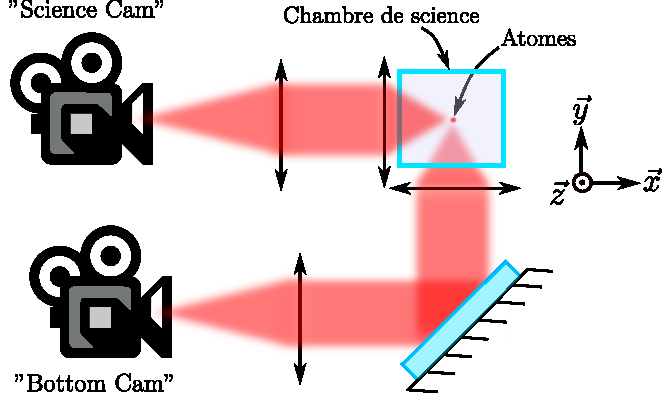
\includegraphics[scale=1]{Fig/BEC_manip/img_science_3.pdf}
\caption{\textbf{Dispositif d'imagerie par fluorescence pour la chambre de science.} Une caméra capte les photons de fluorescence émis par les atomes selon une direction horizontale (\emph{Science Cam}), tandis qu'une autre capte ceux émis vers le bas avec un transport d'image (\emph{Bottom Cam}). Les faisceaux de fluorescence ne sont pas représentés ici (selon l'axe $\vec{z}$).}
\label{fig:img_science}
\end{figure}
Les faisceaux d'imagerie sont à résonance avec la transition $\etatF{2}{} \rightarrow \etat{F'=3}$ et permettent donc de sonder les atomes se trouvant dans l'état $\etatF{2}{}$. Comme pour l'imagerie par absorption, il est aussi possible d'adresser les atomes qui sont dans l'état $\etatF{1}{}$. Pour cela, on superpose aux faisceaux de fluorescence le faisceau repompeur\footnote{Les faisceaux de refroidissement laser et de fluorescence comportent déjà une partie de repompeur: le mélange se fait avant les amplificateurs optiques et il est possible de couper la partie repompeur à l'aide d'un obturateur mécanique, voir figure \ref{fig:table_optique}.}, accordé sur $\etatF{1}{} \rightarrow \etat{F'=2}$ pendant toute la durée de l'impulsion lumineuse, qui est typiquement de 50µs. \\
L'intensité fluorescée captée dans le plan d'imagerie est alors donnée par:
\begin{equation}
I_{\mathrm{fluo}}(y,z)=\frac{\Omega}{4\pi} \frac{s}{1+s} \frac{ \Gamma \hb \omega_0}{2} n_{\mathrm{2D}}(y,z) \text{ ,}
\label{eq:img_fluo}
\end{equation}
avec $\Omega \simeq \pi \ON^2$ l'angle solide dans lequel les photons de fluorescence sont captés par le système d'imagerie d'ouverture numérique $\ON\sim 0.4$. \\
Théoriquement, une seule image suffit à obtenir le profil de densité atomique. Cependant, on décide de prendre une seconde image avec les faisceaux de fluorescence allumés afin de soustraire un éventuel bruit dû à ces faisceaux. Pour des raisons de simplicité de configuration des caméras, on décide aussi de prendre une troisième image du bruit de fond, non utilisée pour le calcul de densité atomique.\\
Étant donné le nombre de paramètres non parfaitement connus dans la formule \ref{eq:img_fluo}, il est nécessaire de calibrer cette méthode d'imagerie. La calibration du nombre d'atomes se fait par comparaison avec l'imagerie par absorption. Si la comparaison est directe dans la première chambre, celle de l'imagerie dans la chambre de science est un peu plus délicate. La méthode retenue par l'équipe consiste à calibrer l'efficacité du transfert par la pince optique à l'aide d'allers-retours pour déterminer le nombre d'atomes attendu dans la seconde chambre.



\usechapterimagefalse
\chapter{Mises à jour de l'expérience}
\label{ch:new_exp}

Nous avons vu dans le chapitre précédent comment nous pouvons générer un condensat de Bose-Einstein, notre source d'onde de matière. Nous avons de plus présenté les principaux mécanismes d'interaction lumière-matière dont nous disposons pour manipuler les atomes, ainsi que la manière dont ces outils sont implémentés sur notre expérience. Une telle plateforme requiert une quantité importante de matériels qu'il est nécessaire d'entretenir, de réparer, voire de remplacer. 

Dans ce nouveau chapitre, nous nous pencherons sur les modifications apportées à l'expérience au cours de ma thèse. Dans la première partie, nous décrirons le nouveau système informatique de contrôle de l'expérience. Dans un second temps, nous caractériserons la lévitation magnétique suite à une avarie sur le circuit de refroidissement à eau. Ensuite, nous nous concentrerons sur le piège dipolaire dont le laser source a été changé. Pour terminer, nous discuterons de l'amélioration de l'évaporation optique permise par les changements précédents.

\section{Contributions au système informatique de l'expérience}
Souvent absente des présentations des expériences, l'informatique occupe pourtant une place primordiale dans les dispositifs d'atomes ultra-froids. Le contrôle simultané et de manière séquentielle des différents équipements de l'expérience, souvent précis à la micro-seconde, n'est possible qu'à l'aide d'un ordinateur disposant de sorties de tension contrôlables. Cet ordinateur, appelé \emph{séquenceur}, constitue le cerveau de l'ensemble du dispositif et contrôle tous les éléments nécessaires à la manipulation des atomes.

Le second aspect où l'informatique se rend indispensable réside dans l'acquisition et le traitement d'images. Le contrôle des caméras et l'extraction des quantités physiques à partir d'images expérimentales nécessite l'utilisation d'un ordinateur et d'au moins un logiciel adapté. 

%De manière générale, les ordinateurs sont les éléments du dispositif avec lesquels l'expérimentateur interagit le plus. Dans cette partie, on présentera donc les changements informatiques ayant eu lieu durant ma thèse.

\subsection{Contrôle de l'expérience: passage à la suite Cicero}
\label{sc:cicero}
Une modification majeure a été le changement du système informatique de contrôle de l'expérience. Le précédent système développé par \emph{André Villing}, ingénieur électronicien du laboratoire maintenant retraité, était piloté de manière programmatique depuis le logiciel Matlab. À des fins de maintenance ainsi que de meilleures performances, le nouveau séquenceur est d'origine commerciale et est basé sur du matériel \emph{National Instruments}:
\begin{itemize}
\item[\textendash] Un ordinateur \emph{PXIe-8840} dans un châssis \emph{PXIe-1078} qui alimente aussi les cartes de génération de signaux.
\item[\textendash] Deux cartes numériques \emph{PXIe-6535} de 32 voies chacune.
\item[\textendash] Deux cartes analogiques \emph{PXIe-6738} de 32 voies $\pm \SI{10}{\volt}$ chacune et codées sur 16 bits.
\end{itemize}
En addition, un circuit logique programmable (\emph{FPGA}) \emph{XEM3001} provenant de \emph{Opal-Kelly} permet de générer une horloge de fréquence variable pour le matériel \emph{National Instruments}. La justification de cette horloge de fréquence variable réside dans la grande variabilité de la durée des différentes étapes d'une expérience d'atomes ultra-froids: l'expérience peut rester dans le même état plusieurs secondes (pendant le chargement d'un MOT par exemple) tout comme elle doit pouvoir changer d'état pendant quelques microsecondes seulement (pendant l'imagerie par exemple). Une séquence durant typiquement \SI{30}{\second} discrétisée toutes les microsecondes pour un minimum d'une cinquantaine de voies saturerait alors la mémoire de l'ordinateur. 

L'écriture de la séquence se fait à présent grâce à la suite \emph{Cicero Word Generator}, développée au \emph{MIT} dans le groupe de Wolfgang Ketterle \citep{keshet2013distributed}. Cette suite comporte deux logiciels qui fonctionnent selon une architecture client/serveur. Le client \emph{Cicero} est une interface graphique dans laquelle l'utilisateur écrit une séquence sous la forme d'une suite d'étapes comme illustré figure \ref{fig:cicero}. Au lancement d'un cycle expérimental, \emph{Cicero} envoie les données de séquence au serveur \emph{Atticus} qui calcule alors les consignes des cartes ainsi que l'horloge variable à appliquer \citep{keshet2008cicero}.

\begin{figure}
\centering
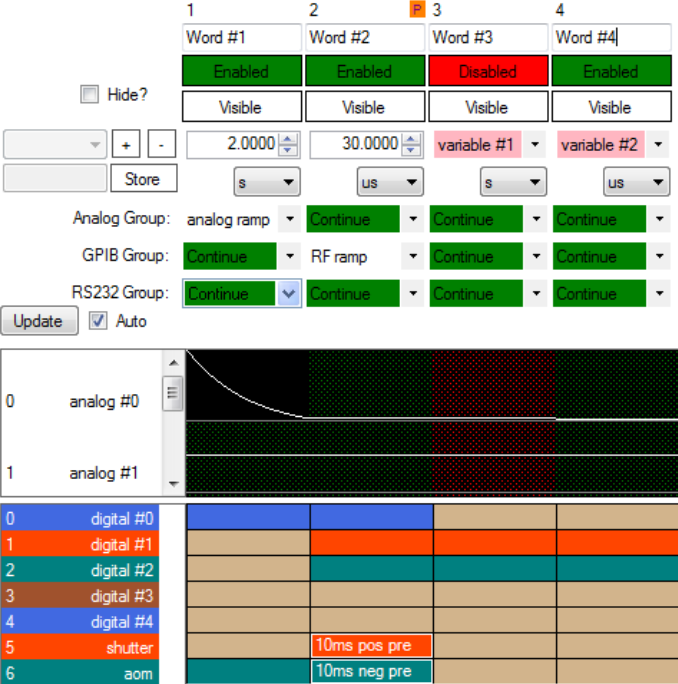
\includegraphics[width=0.7\textwidth]{Fig/Modif_exp/cicero.png}
\caption{\textbf{Capture d'écran de \emph{Cicero}.} Une séquence est une suite d'étapes (des colonnes dans l'interface) pendant lesquelles on peut faire des motifs avec les voies analogiques. Les voies numériques changent d'état en général entre deux étapes. Il est possible de désactiver certaines étapes et d'utiliser des variables. Figure tirée de \citep{keshet2013distributed}.}
\label{fig:cicero}
\end{figure}

Grâce à cette architecture client/serveur, il est possible de connecter une interface \emph{Cicero} à plusieurs serveurs. Nous avons ainsi développé un serveur supplémentaire\footnote{Une attention particulière a été accordée à n'apporter aucune modification au code source de la suite \emph{Cicero} excepté dans l'environnement de ce serveur. Les environnements de \emph{Cicero}, \emph{Atticus} et les environnements communs n'ont subit aucun changement pour s'assurer de la compatibilité avec la version compilée 1.64rev7 de la suite.} afin de faciliter notre traitement de données. Celui-ci enregistre les principales données de séquence\footnote{Il s'agit du nom de séquence, de l'heure de lancement, de l'ensemble des variables, des étapes, des groupes d'étapes et de la dernière consigne du piège dipolaire avant le temps de vol.} à chaque cycle.

Ce changement de séquenceur ouvre de nouvelles perspectives en augmentant le nombre de voies utilisables (16 voies analogiques codées sur 12 bits et 48 voies numériques avec le précédent système) tout en permettant la génération de signaux arbitraires (auparavant limités à des morceaux de rampes).


\subsection{Développement d'une nouvelle interface d'acquisition et de traitement d'images}
Comme présenté dans la partie \ref{sc:imagerie}, les caméras que l'on utilise sur l'expérience sont configurées et contrôlées via le logiciel Matlab. En particulier, l'acquisition et le traitement des images se faisait à l'aide d'une interface commune avec l'ancien séquenceur. Son remplacement a donc eu un impact important sur le fonctionnement de la partie imagerie. 

En conséquence, nous avons développé une nouvelle interface graphique permettant de configurer les caméras, d'acquérir et de traiter les images, d'enregistrer les données et de contrôler tout les éléments non adressables depuis \emph{Cicero}. Le cahier des charges de cette nouvelle interface est donc le suivant:
\begin{itemize}
\item[\textendash] Gestion des trois caméras, avec possibilité de faire l'acquisition simultanée sur les deux caméras de la chambre de science.%\footnote{Un ordinateur supplémentaire était nécessaire pour le contrôle de la caméra \textit{bottom}, pilotée via une autre interface. Il fallait donc synchroniser ces deux ordinateurs qui enregistraient chacun leurs fichiers de données.}.
\item[\textendash] Imagerie par absorption et par fluorescence.
\item[\textendash] Calcul en direct des grandeurs physiques pour chaque image.
\item[\textendash] Lecture des données de Cicero récupérées grâce au serveur que nous avons développé.
\item[\textendash] Programmation en début de cycle des sources radio-fréquence utilisées pour l'évaporation radio-fréquence et la manipulation de l'état de spin dans la chambre de science\footnote{Cette programmation en début de cycle est rendue possible grâce à l'utilisation d'un \emph{FileSystemWatcher} provenant d'une bibliothèque .NET utilisable dans Matlab. Un fichier texte contenant les données du cycle en cours est généré en début de séquence par le serveur que nous avons développé, déclenchant alors automatiquement sa lecture par l'interface.}.
\item[\textendash] Enregistrement de l'ensemble des données et des paramètres du cycle pour un futur traitement.
\end{itemize}
L'utilisation de cette nouvelle interface a donc permis de centraliser les données générées par l'acquisition d'images. De plus, ce changement a permis de s'affranchir de plusieurs canaux de communication, les libérant ainsi pour le contrôle d'instruments. Enfin, l'utilisation et le fonctionnement de cette nouvelle interface Matlab sont simplifiés, permettant d'opérer avec une plus grande facilité les changements à venir sur l'expérience.











\section{Calibration de la lévitation magnétique}
\label{sc:levitation}
Comme présenté partie \ref{sc:chambre_science}, la lévitation magnétique est un élément essentiel de notre expérience. En plus d'être un pré-requis pour l'étude de la localisation d'Anderson à trois dimensions, celle-ci nous permet de manière plus générale d'obtenir des échantillons particulièrement froids. Son bon fonctionnement est donc crucial pour notre expérience. Notons de plus que dans le cadre de l'étude la transition d'Anderson à énergie résolue, il s'avère nécessaire d'avoir une connaissance fine du potentiel magnétique dans lequel les atomes évoluent.% Importance de calibrer proprement tous les champs magnétiques.

Malheureusement, la formation d'un bouchon à base de précipités métalliques dans le circuit de refroidissement de la lévitation a conduit au démontage d'une partie importante du système de la lévitation. Les modifications apportées avant remontage ayant pu conduire à une modification du comportement magnétique du système, une nouvelle calibration fine des champs magnétiques a été menée.

Dans cette partie, nous présenterons dans un premier temps notre système de lévitation ainsi que les modifications qui y ont été apportées. Ensuite, nous nous pencherons sur les méthodes utilisées pour calibrer le système après sa réinstallation sur l'expérience, en commençant par  une spectroscopie radio-fréquence permettant de calibrer les champs magnétiques, puis à l'aide d'expériences d'oscillations afin de caractériser le potentiel magnétique.




\subsection{Implémentation de la lévitation magnétique}
\label{sc:implementation_levitation}
L'ensemble du système de la lévitation magnétique a été développé alors que l'équipe se dirigeait vers les expériences de localisation d'Anderson à trois dimensions. De nombreux détails de conception pourront être retrouvés dans le manuscrit de thèse d'Alain Bernard \citep{bernard2010transport}, mais rappelons les éléments nécessaires à la suite.


\begin{figure}
\centering
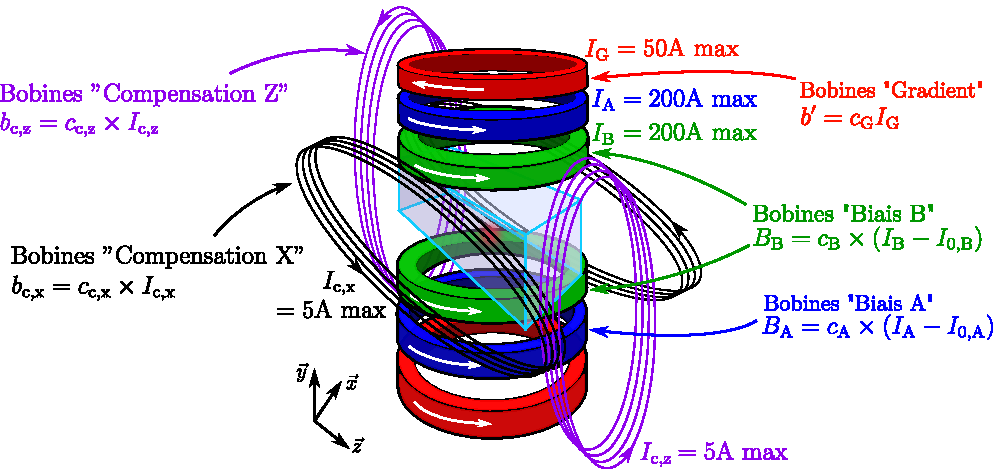
\includegraphics[width=\textwidth]{Fig/modif_exp/geometrie_levitation.pdf}
\caption{\textbf{Géométrie de la lévitation magnétique.} Le système de lévitation magnétique se compose d'un grand nombre de bobines. Les bobines représentées en rouge génèrent un gradient magnétique $b'$ suivant la direction verticale $\vec{y}$ afin de lutter contre la gravité. Les bobines en bleu et en vert permettent de générer de forts champs magnétiques de biais dans la direction verticale. Les bobines violettes et noires permettent quant à elles de générer de petits champs horizontaux dans les directions $\vec{z}$ et $\vec{x}$ respectivement.}
\label{fig:geometrie_levitation}
\end{figure}

La lévitation magnétique est composée d'un grand nombre de paires de bobines, illustrées figure \ref{fig:geometrie_levitation}. Les deux paires de bobines les plus proches de la cellule, en bleu et en vert, permettent de créer un champ de biais selon la direction verticale $\vec{y}$ au niveau des atomes. Les bobines de \emph{Biais A}, en bleu, se trouvent dans une configuration légèrement plus éloignée que la configuration de Helmholtz, tandis que les bobines de \emph{Biais B}, en vert, sont légèrement rapprochées par rapport à la configuration de Helmholtz. La paire la plus éloignée, en rouge, permet de créer un gradient magnétique afin de suspendre les atomes contre la gravité. 

Le champ magnétique au niveau des atomes peut alors être écrit
\begin{equation}
\mathbf{B}=\left[ \Bzero - b'y + b'' \left( y^2 - \frac{x^2+z^2}{2} \right) \right] \vec{y} + \left( \frac{b'}{2}x \right) \vec{x} + \left( \frac{b'}{2}z \right) \vec{z} \text{ ,}
\label{eq:champ_mag_levitation}
\end{equation}
où $b'$ correspond au gradient magnétique généré par les bobines de \emph{Gradient}. Le  paramètre $b''$ est la courbure du champ généré par l'écart des bobines de biais à la configuration de Helmholtz. La valeur du champ au centre est donnée par $\Bzero$.
Le potentiel magnétique étant proportionnel à la norme du champ, celle-ci est donnée à l'ordre deux par
\begin{equation}
B=\Bzero -b' y + b'' y^2 +\frac{1}{2} \left( \frac{b'^2}{4 \Bzero} - b'' \right) \left( x^2 + z^2 \right) \text{ ,}
\label{eq:norme_levitation}
\end{equation}
où le terme linéaire est celui qui permet de compenser la gravité.

Les gradients dans les directions horizontales $\vec{x}$ et $\vec{z}$ proviennent de la conservation du flux magnétique, et rendent le potentiel de lévitation très sensible aux biais horizontaux. Il est donc important de contrôler finement le champ transverse. À ces fins, plusieurs bobines supplémentaires sont utilisées pour générer de faibles champs de compensation dans les directions $\vec{x}$ (bobines représentées en noir sur la figure \ref{fig:geometrie_levitation}) et $\vec{z}$ (en violet).



 

Les courants parcourant les bobines de lévitations sont générés à l'aide d'alimentations ultra-stables\footnote{Ces alimentations sont stables au \SI{}{\milli\ampere} près.} permettant de délivrer jusqu'à \SI{200}{\ampere} pour les bobines de biais, et jusqu'à \SI{50}{\ampere} pour les bobines de gradient. Les bobines sont reliées aux alimentations au travers de boitiers d'isolement à commutation rapide ne laissant passer que les courants positifs à l'aide de diodes. Les alimentations des bobines de compensation sont quant à elles limitées à environ \SI{5}{\ampere}.

L'objectif de la calibration de la lévitation magnétique est donc de déterminer les propriétés du potentiel de lévitation, et donc les grandeurs caractéristiques des champs magnétiques apparaissant dans l'équation \ref{eq:champ_mag_levitation}, en fonction des courants parcourant les bobines générant ces champs. En particulier, nous chercherons à établir des relations linéaires entre les différents champs et les courants:
\begin{align}
&B_{\mathrm{A}}=c_{\mathrm{A}} \times (I_{\mathrm{A}}-I_{\mathrm{0,A}}) \quad &&\text{et}\quad B_{\mathrm{B}}=c_{\mathrm{B}} \times (I_{\mathrm{B}}-I_{\mathrm{0,B}}) \text{ ,}\label{eq:calibration_biais_lev}\\
&b_{\mathrm{A}}'' = c_{\mathrm{A}}'' \times (I_{\mathrm{A}}-I_{\mathrm{0,A}}) \quad &&\text{et} \quad b_{\mathrm{B}}'' = c_{\mathrm{B}}'' \times (I_{\mathrm{B}}-I_{\mathrm{0,B}}) \text{ ,}\label{eq:calibration_courbure_lev}\\
&b_{\mathrm{c,x}}=c_{\mathrm{c,x}} \times I_{\mathrm{c,x}} \quad &&\text{et}\quad b_{\mathrm{c,z}}= c_{\mathrm{c,z}} \times I_{\mathrm{c,z}} \text{ ,}\label{eq:calibration_biais_comp}\\
&b'= c_{\mathrm{G}} \times I_{\mathrm{G}} \text{ ,}\label{eq:calibration_gradient} && 
\end{align}
où les grandeurs $c_{\mathrm{i}}$ correspondent aux facteurs de calibration et les courants $I_{\mathrm{0,i}}$ correspondent aux courants seuils liés aux boitiers d'isolement contenant des diodes. La calibration précise des champs de biais se fera à l'aide d'une spectroscopie radio-fréquence des déplacements des sous-niveaux Zeeman, tandis que la détermination des courbures et du gradient se feront à l'aide de la mesure des caractéristiques du potentiel de lévitation.



\subsection{Intervention sur le circuit de refroidissement}
En raison des très gros courants pouvant circuler dans les bobines de lévitation, celles-ci sont refroidies par l'intermédiaire de leur support à l'aide d'une circulation d'eau. En effet, ces supports en aluminium, disposés de part et d'autre de la cellule, comportent chacun trois bobines scellées à l'aide d'une résine. Ces supports agissent alors comme un réservoir thermique pour les bobines.

Cependant, la formation d'un précipité métallique à l'intérieur de ces supports a privé les bobines de lévitation de refroidissement, indispensable pour un fonctionnement à haut courant\footnote{Les bobines de chaque support absorbent une puissance de plusieurs \SI{}{\kilo\watt} lors d'une lévitation très décomprimée, c'est-à-dire à haut courant \citep{bernard2010transport}.}. Le retrait de ce bouchon a nécessité le démontage d'une partie du système de lévitation ainsi qu'une intervention lourde sur les supports en aluminium. Initialement, l'eau circulait dans des trous borgnes percés dans le support en aluminium (représentés en rouge figure \ref{fig:refroidissement_levitation}.a), dont l'étanchéité était assurée par des vis montées serrées et scellées à l'aide d'une colle anaérobie. Le débouchage a entraîné la destruction de ces vis.

Après de nombreux travaux de débouchage et d'étanchéité, ce refroidissement est à présent effectué par le contact entre le support en aluminium et la circulation d'eau dans deux tubes en cuivre encastrés\footnote{Le débouchage des trous leur a fait perdre leur étanchéité, et après plusieurs essais infructueux, nous avons retenu la solution de deux tubes de cuivre encastrés et débouchants. De nombreux tests électriques ont été menés sur les bobines tout au long de leur maintenance pour s'assurer de l'absence de dégradation.}, visibles figure \ref{fig:refroidissement_levitation}.a. On comprend aisément que ce nouveau refroidissement sera moins efficace que précédemment, celui-ci se faisant par le biais de deux contacts thermiques et la surface de contact étant diminuée. Néanmoins, on observe une réelle efficacité de refroidissement comme en témoigne la figure \ref{fig:refroidissement_levitation}.b.

\begin{figure}
\centering
\includegraphics[width=\textwidth]{Fig/Modif_exp/levitation_refroidissement.pdf}
\caption{\textbf{a: Refroidissement de la lévitation magnétique.} L'un des supports des bobines de la lévitation est maintenant refroidi à l'aide de deux tubes en cuivre le traversant. Auparavant, l'eau circulait directement dans le support dans un circuit percé illustré par les traits rouges. Les tubes en cuivre ont pu être installés en rendant une partie de ce circuit débouchant. \textbf{b: Efficacité de refroidissement.} Ces mesures ont été réalisées dans des conditions proches de véritables cycles expérimentaux. Le même courant a été appliqué pendant \SI{10}{\second} sur toutes les bobines à la fin de séquences habituelles. La température a été mesurée après la répétition d'au moins 30 cycles et en s'assurant de sa stabilisation.}
\label{fig:refroidissement_levitation}
\end{figure}



































\subsection{Calibration des champs par radio-fréquences}
\label{sc:levitation_RF}


%Cette dernière stratégie rend possible l'approche novatrice de désordre dépendant de l'état interne, qui impose de travailler à un \emph{biais magique} $\magicB=\SI{3.229}{\gauss}$ pour lequel les susceptibilités magnétiques des états $\etatF{1}{-1}$ et $\etatF{2}{+1}$ sont identiques \citep{denechaud2018vers}. La valeur précise de ce champ magique demande alors une connaissance fine des caractéristiques du dispositif de génération des champs magnétiques de l'expérience.

Afin de déterminer très précisément le champ magnétique généré par les bobines de biais, la mesure de ces champs a été effectuée par spectroscopie radio-fréquence. Son principe repose sur le transfert de population entre l'état d'origine $\etatF{1}{-1}$ et les états $\etatF{2}{\lbrace -2,-1,0\rbrace}$ accessibles\footnote{Au cours de cette étude, nous nous sommes rendus compte que le nuage subissait une dépolarisation peuplant les trois sous états Zeeman $\etatF{1}{\lbrace-1,0,1}$, faisant alors apparaître sept résonances visibles sur la figure \ref{fig:calibration_RF}. Cette dépolarisation a été confirmée par une analyse Stern-Gerlach. Depuis, cette dépolarisation a pu être évitée.}, dont la séparation en énergie avec l'état d'origine dépend du champ magnétique en vertu de la formule de Breit-Rabi \ref{eq:Breit-Rabi}. Ainsi, lorsque la radio-fréquence satisfait la condition de résonance $\nu_{\mathrm{RF}}=\deltahf + \delta \nu (B)$ avec $\delta \nu (B)$ le décalage dû au champ magnétique, une partie des atomes sera transférée dans l'un des sous-états de $\etatF{2}{}$. Le principe de cette spectroscopie est illustré figure \ref{fig:calibration_RF}.a.

\begin{figure}
\centering
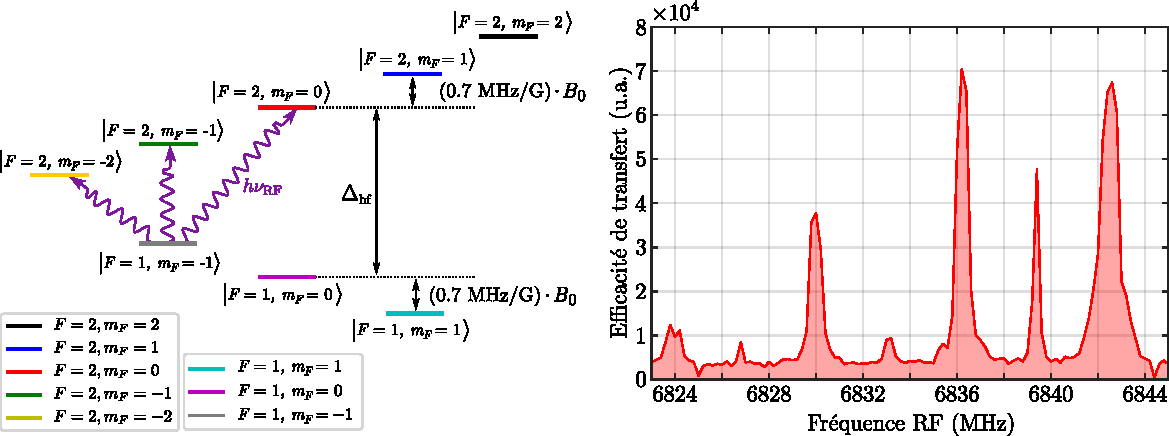
\includegraphics[width=\textwidth]{Fig/Modif_exp/levitation_RF.pdf}
\caption{\textbf{a: Principe de la spectroscopie radio-fréquences}. En balayant la fréquence de l'onde radio-fréquence appliquée, on adresse les différentes transitions entre sous-états Zeeman de $\protect\etatF{1}{}$ et $\protect\etatF{2}{}$ dont la séparation dépend du champ magnétique. \textbf{b: Spectre radio-fréquence.} Lorsque l'onde radio-fréquence est à résonance, on transfère des atomes initialement dans l'état $\protect\etatF{1}{}$ vers l'état $\protect\etatF{2}{}$. La présence de sept résonances équidistantes indique une dépolarisation du nuage, les règles de sélection imposant $\Delta \mf = \lbrace \pm 1,0 \rbrace$. Les trois premières résonances correspondent à celles illustrées sur la figure \textbf{a}. Le champ magnétique extrait de ce spectre est d'environ $\SI{4.4}{\gauss}$.}
\label{fig:calibration_RF}
\end{figure}



En relevant le spectre des transitions radio-fréquences\footnote{Cette mesure a été effectuée dans le piège dipolaire croisé, et étant donné le très grand désaccord du faisceau de piégeage, on peut considérer que les déplacements lumineux induits sur les états $\etatF{1}{}$ et $\etatF{2}{}$ sont identiques. La séparation entre les états considérés n'en sera donc pas affectée. Il est ensuite possible d'imager sélectivement les atomes transférés dans l'état $\etatF{2}{}$ par fluorescence en coupant la partie du faisceau d'imagerie provenant du laser repompeur.} en balayant la fréquence rayonnée $\nu_{\mathrm{RF}}$ comme illustré figure \ref{fig:calibration_RF}.b, on accède ainsi à la valeur du champ magnétique au niveau des atomes en déterminant $\delta\nu(B)$, qu'il est possible d'approximer par le décalage par effet Zeeman linéaire dans un régime de bas champ:
\begin{equation}
\delta \nu (B)\simeq -(m_{\mathrm{F_2}} - m_{\mathrm{F_1}} ) \times \SI{0.7}{\mega\hertz\per\gauss} \times B \text{ ,}
\label{eq:levitation_RF}
\end{equation}
où le champ $B$ correspond à la norme du champ magnétique total, c'est-à-dire le champ de biais étudié et les champs naturellement présents $\mathbf{b}_{\mathrm{0}}$: 
\begin{equation}
B=\sqrt{(b_{\mathrm{c,x}}+b_{\mathrm{0x}})^2+(B_{\mathrm{A}}+B_{\mathrm{B}}+b_{\mathrm{0y}})^2+(b_{\mathrm{c,z}}+b_{\mathrm{0z}})^2} \text{ .}
\end{equation}

En réalisant cette opération pour différents courants pour chacune des bobines de biais, il nous est possible de déterminer les calibrations des champs magnétiques \ref{eq:calibration_biais_lev} et \ref{eq:calibration_biais_comp}. En particulier, le comportement à très bas champ nous permet de déterminer les différentes composantes $b_{\mathrm{0i}}$ du champ rémanent, souvent négligeable devant le champ rayonné pour des courants usuels. L'ensemble des calibrations des champs de biais est donné table \ref{tb:levitation_RF}.
 

\renewcommand{\arraystretch}{1.1}
\begin{table}[!h]
{\rowcolors{2}{white}{MainColor!10}
\begin{center}
\begin{tabular}{ c|c }
%\hline
{\color{MainColor}\textbf{Grandeur}} & {\color{MainColor}\textbf{Valeur}} \\
%\hline
Calibration Biais A $c_{\mathrm{A}}$ & \SI{4.704}{\gauss\per\ampere} \\
%\hline
Calibration Biais B $c_{\mathrm{B}}$ & \SI{6.180}{\gauss\per\ampere} \\
%\hline
Calibration Compensation X $c_{\mathrm{x}}$ & \SI{4.903}{\gauss\per\ampere} \\
%\hline
Calibration Compensation Z $c_{\mathrm{z}}$ & \SI{4.969}{\gauss\per\ampere} \\
%\hline
Courant seuil Biais A $I_{\mathrm{0,A}}$ & $< \SI{1}{\milli\ampere}$ \\
%\hline
Courant seuil Biais B $I_{\mathrm{0,B}}$ & \SI{0.345}{\ampere} \\
%\hline
Champ rémanent $b_{\mathrm{0x}}$ & \SI{0.089}{\gauss} \\
%\hline
Champ rémanent $b_{\mathrm{0y}}$ & \SI{0.426}{\gauss} \\
%\hline
Champ rémanent $b_{\mathrm{0z}}$ & \SI{-0.416}{\gauss} \\
%\hline
\end{tabular}
\end{center}}
\caption{\textbf{Calibration des champs de biais dans la chambre de science.} Les champs rémanents $b_{\mathrm{0i}}$ correspondent aux champs extérieurs dans la direction $\vec{i}$. Le champ magnétique généré dans la cellule est proportionnel au courant parcourant les bobines $B_{\mathrm{i}} = c_{\mathrm{i}} \times (I_{\mathrm{i}}-I_{\mathrm{0,i}})$ avec $I_{\mathrm{0,i}}$ le courant seuil, qui correspond à la consigne minimale à appliquer pour que le courant circule dans les bobines.}
\label{tb:levitation_RF}
\end{table}
















\subsection{\'Etude du potentiel de lévitation}
\label{sc:oscillations_levitation}
Nous avons vu précédemment 
Il est important de maîtriser le potentiel de lévitation magnétique en fonction du champ. Caractérisation des fréquences de piégeage et du centre du potentiel. 
Cette considération est d'autant plus importante puisque nous envisageons de réaliser un passage adiabatique d'une lévitation à bas champ à une lévitation à fort champ.




\paragraph*{Potentiel de lévitation}
Comme nous l'avons mentionné dans le chapitre précédent, il existe une limite pour les fréquences de piégeage (formule \ref{eq:theoreme_wing}) qui décroît avec la norme du champ magnétique. Une stratégie usuelle est donc de créer un champ aussi fort que possible, qui est d'environ \SI{2000}{\gauss} avec notre système (correspondant à un courant maximal de \SI{200}{\ampere}). Pour de tels champs, le potentiel magnétique n'est plus décrit par l'effet Zeeman linéaire, mais par la formule de Breit-Rabi \ref{eq:Breit-Rabi}. En revanche, pour une petite zone autour du centre du potentiel de lévitation, on peut simplifier l'étude en supposant que le champ change peu $B\simeq \Bzero$. On peut ainsi définir un facteur de Landé local:
\begin{equation}
\gftilde(\Bzero)=\frac{1}{\mf \mub} \frac{\mathrm{d}E}{\mathrm{d}B}(\Bzero) \text{ ,}
\label{eq:facteur_lande_local}
\end{equation}
obtenu à l'aide d'un développement limité de la formule de Breit-Rabi \ref{eq:Breit-Rabi} autour du champ $\Bzero$. La physique derrière cette approche est de considérer l'effet Zeeman linéaire sur un état dont la susceptibilité magnétique dépend du champ de Biais $\Bzero$. Cela se traduit par une correction du potentiel magnétique \ref{eq:potentiel_mag} qu'il est possible de réécrire sous la forme:
\begin{equation}
U_{\mathrm{mag}}(\mathbf{x})=m_{\mathrm{F}}\gftilde(\Bzero)\mub B(\mathbf{x}) \text{ ,}
\label{eq:potentiel_levitation}
\end{equation}
dans une zone proche autour du centre du potentiel de lévitation.




\paragraph*{Gradient de lévitation}
À l'aide du potentiel \ref{eq:potentiel_levitation}, il nous est possible de déterminer la valeur du gradient nécessaire pour compenser la gravité:
\begin{equation}
b'=\frac{mg}{\mf \gftilde(\Bzero) \mub} \text{ ,}
\label{eq:gradient_levitation}
\end{equation}
qui, de manière générale, dépend donc du biais magnétique au niveau des atomes.
Cette dépendance est illustrée figure \ref{fig:levitation_etats} pour les différents états internes d'intérêt dans cette thèse: $\etatF{1}{-1}$, $\etatF{2}{+1}$ et $\etatF{2}{-2}$. 

Notons trois résultats remarquables de la figure \ref{fig:levitation_etats}: 
\begin{itemize}
\item[\textendash] L'état $\etatF{2}{-2}$ nécessite un gradient indépendant du biais magnétique pour être lévité. 
\item[\textendash] Les états $\etatF{1}{-1}$ et $\etatF{2}{+1}$ sont lévités pour le même gradient à bas champ. Plus précisément, la susceptibilité magnétique de ces états est égale uniquement pour un \emph{champ magnétique magique} $\Bzero^*=\SI{3.229}{\gauss}$\footnote{Ce champ magique est dû au spin nucléaire. Une dérivation de ce champ peut être trouvée dans la référence \citep{denechaud2018vers}.}, impliquant que ces états ont le même comportement magnétique. Cela se traduit notamment par une lévitation simultanée.
\item[\textendash] L'état $\etatF{1}{-1}$ ne peut être lévité que pour des champs inférieurs à environ \SI{150}{\gauss} en raison de la limitation de courant (\SI{50}{\ampere}) de l'alimentation des bobines de gradient. En effet, le gradient nécessaire pour contrer la gravité augmente avec le champ magnétique.
\end{itemize}
Plusieurs stratégies expérimentales de lévitation s'offrent alors. La première provient de l'état $\etatF{2}{-2}$ qui peut être lévité tout en gardant la valeur du champ de biais comme un degré de liberté, on peut alors réaliser des lévitations très décomprimées. Il s'agit de l'approche utilisée pour la mesure du temps de diffusion élastique, présentée chapitre \ref{ch:TauS_PRL}. Une autre possibilité est que les états $\etatF{1}{-1}$ et $\etatF{2}{+1}$ peuvent coexister dans le champ de lévitation, on peut ainsi utiliser l'état interne de l'atome comme degré de liberté tout en étant lévité. Cette stratégie a par exemple été utilisée pour la mesure des fonctions spectrales \citep{volchkov2018measurement}.

\begin{figure}
\centering
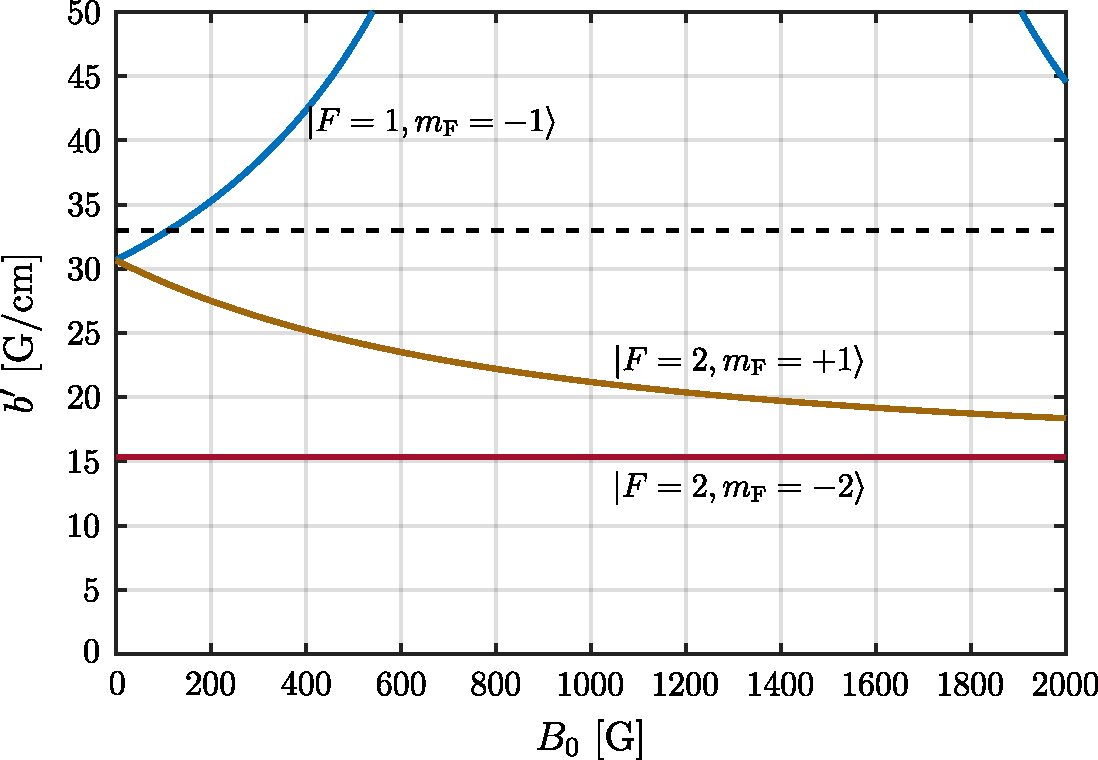
\includegraphics[width=0.7\textwidth]{Fig/Modif_exp/levitation_etats.pdf}
\caption{\textbf{Gradient nécessaire pour compenser la gravité en fonction du biais magnétique.} La valeur du gradient magnétique à appliquer pour léviter dépend de l'état électronique, mais aussi du biais magnétique $\protect\Bzero$ par la formule de Breit-Rabi. L'état $\protect\etatF{1}{-1}$ ne peut être lévité qu'à bas champ (courbe bleue), l'alimentation des bobines de gradient ne pouvant délivrer plus de \SI{50}{\ampere} (limite tracée en pointillés). Les états $\protect\etatF{2}{+1}$ (courbe marron) et $\protect\etatF{2}{-2}$ (courbe bordeau) peuvent être lévités pour n'importe quelle valeur du biais.}
\label{fig:levitation_etats}
\end{figure}

Enfin, il est possible de déduire une calibration des bobines de gradient de la relation \ref{eq:gradient_levitation} entre le gradient magnétique et le biais $\Bzero$. En identifiant des couples $\lbrace I_{\mathrm{Gradient}}, I_{\mathrm{Biais}} \rbrace$ permettant de compenser précisément la gravité, on parcourt ainsi la courbe de la figure \ref{fig:levitation_etats} pour l'état $\etatF{1}{-1}$. On détermine alors le facteur de calibration $c_{\mathrm{G}}=\SI{0.66}{\gauss\per\centi\metre\per\ampere}$.




\paragraph*{Fréquences de la lévitation}
De manière générale, nous avons besoin de caractériser le piégeage résiduel de la lévitation, celui-ci pouvant influencer un piège optique fortement décomprimé dans une configuration à bas champ, et il est nécessaire d'estimer le potentiel résiduel des atomes en expansion dans le désordre dans le cas d'une configuration à fort champ.

Pour l'état $\etatF{1}{-1}$ en particulier, dans lequel nous créons notre condensat de Bose-Einstein, le centre de masse du nuage décrit des oscillations autour du centre de la lévitation dont les fréquences peuvent être trouvées à l'aide de la norme du champ magnétique \ref{eq:norme_levitation} et du potentiel magnétique \ref{eq:potentiel_levitation}:
\begin{equation}
\omega_x^2=\omega_z^2=\left| \frac{\mf \gftilde \mub}{m} \left( \frac{b'^2}{4 \Bzero} - b'' \right) \right|
\quad \text{et} \quad
\omega_y^2= \left| \frac{2 \mf \gftilde \mub }{m} b'' \right| \text{ .}
\label{eq:frequences_leviation}
\end{equation}
Nous allons donc utiliser ces oscillations naturelles du nuage (une fois relâché après extinction du piège dipolaire) dans le piège de la lévitation magnétique pour caractériser le potentiel de lévitation en terme de centre et de courbure.%L'exploitation de ces oscillations fournit donc de précieux renseignements quant à la position du centre de la lévitation, mais aussi quant à la forme du potentiel magnétique dans lequel les atomes évoluent. 

En particulier, la mesure des fréquences de la lévitation permet de déterminer la courbure des champs générés par les bobines de biais A et de biais B. L'influence de ces courbures est représentée figure \ref{fig:frequences_levitation} pour les champs de biais A et de biais B. Pour un courant suffisamment grand, le terme de courbure $b_{\mathrm{i}}''= c_{\mathrm{i}}'' \times (I_{\mathrm{i}}-I_{\mathrm{0,i}})$ n'est plus négligeable devant celui de gradient, atténué par le biais. En effet, la comparaison des fréquences expérimentales aux fréquences \ref{eq:frequences_leviation} à courbure nulle $b''=0$ montre un fort désaccord dans la zone des courants les plus hauts, tandis qu'un modèle tenant compte d'une courbure proportionnelle au courant décrit correctement cette zone (voir figure \ref{fig:frequences_levitation}.b). On peut alors extraire le facteur de conversion courbure/courant $c_{\mathrm{i}}''$.




\begin{figure}
\centering
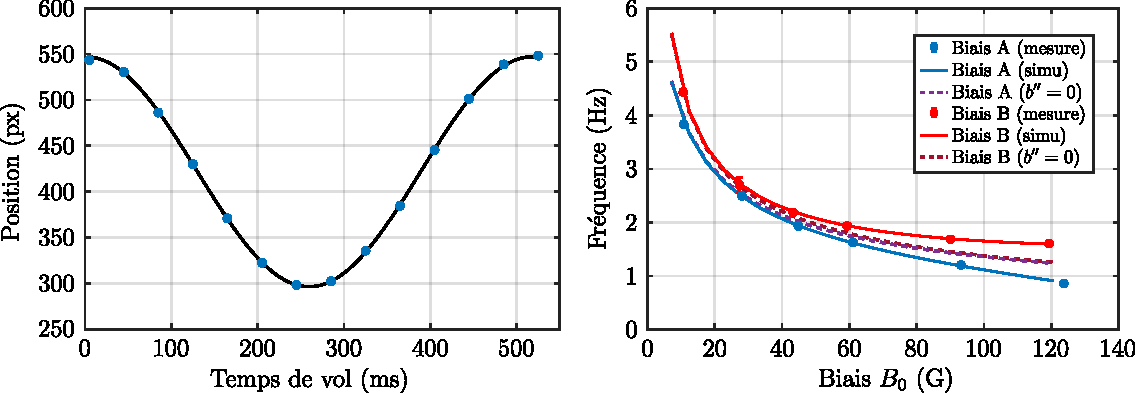
\includegraphics[width=\textwidth]{Fig/Modif_exp/oscillation_levitation.pdf}
\caption{\textbf{a: Oscillation du nuage dans la lévitation magnétique.} Le nuage, initialement dans le piège optique, est relâché décentré par rapport au potentiel de la lévitation. Il acquiert alors un mouvement oscillatoire autour du centre de la lévitation pendant le temps où la gravité est compensée. \textbf{b: \'Evolution des fréquences de piégeage de la lévitation.} Les fréquences mesurées (points) diminuent avec l'augmentation de $\Bzero$ et sont comparées à des simulations du potentiel (lignes continues) afin de calibrer le champ créé par les bobines. L'influence des courbures est visible pour les plus champs les plus intenses, les simulations en absence de courbure (courbes tiretées) montrant alors une déviation par rapport aux données.}
\label{fig:frequences_levitation}
\end{figure}


%\renewcommand{\arraystretch}{1.1}
\begin{table}[!h]
\begin{center}
{\rowcolors{2}{white}{MainColor!10}
\begin{tabular}{ c|c }
%\hline
{\color{MainColor} \textbf{Courbure}} & {\color{MainColor} \textbf{Valeur}} \\
%\hline
Gradient $c_{\mathrm{G}}$ & \SI{0.66}{\gauss\per\centi\metre\per\ampere} \\
%\hline
Biais A $c_{\mathrm{A}}''$ & \SI{4e-2}{\gauss\centi\metre^{-2}\ampere^{-1}} \\
%\hline
Biais B $c_{\mathrm{B}}''$ & \SI{-7e-2}{\gauss\centi\metre^{-2}\ampere^{-1}} \\
%\hline
\end{tabular}}
\end{center}
\caption{\textbf{Calibration du potentiel de lévitation magnétique.} Les bobines de lévitation générant les champs de biais n'étant pas en configuration de Helmholtz, elles créent donc une courbure de champ magnétique au niveau des atomes. Cette courbure dépend de la géométrie des bobines ainsi que du courant les parcourant $b_{\mathrm{i}}''= c_{\mathrm{i}}'' \times (I_{\mathrm{i}}-I_{\mathrm{0,i}})$.}
\label{tb:courbures_levitation}
\end{table}

On peut alors estimer les fréquences de piégeage (ou d'anti-piégeage pour l'état $\etatF{2}{-2}$) dans les configurations expérimentales d'intérêt. Pour le champ magique $\magicB$, les états $\etatF{1}{-1}$ et $\etatF{2}{+1}$ sont soumis à un piégeage de fréquence d'environ \SI{5}{\hertz} par les bobines de biais A tandis que dans le régime de champ fort, nécessaire pour obtenir les décompressions maximales qu'offre notre système, la fréquence de piégeage (anti-piégeage) pour l'état $\etatF{2}{+1}$ ($\etatF{2}{-2}$) est diminuée jusqu'à \SI{0.20}{\hertz} (\SI{0.18}{\hertz}) sous un champ de \SI{2000}{G} \citep{bernard2010transport}.





\paragraph*{Centre de la lévitation}
Dans le cas d'un système idéal, le centre du potentiel magnétique correspond au centre géométrique des bobines. Cependant, on comprend aisément qu'en raison du gradient magnétique de lévitation, la position horizontale du centre du potentiel magnétique sera très sensible aux perturbations extérieures ainsi qu'aux défauts de positionnement des bobines. en particulier, on peut s'attendre à ce qu'un champ horizontal $b_{\mathrm{z}}$ entraîne un déplacement $\Delta z=-2b_{\mathrm{z}}/b'$ du centre du potentiel. Afin d'éviter de mettre le nuage en mouvement après relâchement du piège optique, on utilise alors des champs de compensation générés à l'aide de bobines supplémentaires et dont le rôle est de repositionner le centre du potentiel magnétique sur le nuage. 

Le champ permettant de déplacer le potentiel est donc la somme d'un champ naturellement présent et du champ de compensation:
\begin{equation}
b_{\mathrm{i}}=b_{\mathrm{0,i}}+c_{\mathrm{c,i}} \times I_{\mathrm{c,i}} \quad \text{avec} \quad i=\lbrace x,z \rbrace \text{ .}
\end{equation}
Les mesures des différents termes de ce champ ont été effectuées à l'aide de radio-fréquences, comme décrit section \ref{sc:levitation_RF}. 

Il est alors possible de généraliser l'expression \ref{eq:champ_mag_levitation} du champ magnétique total sous l'effet d'une petite composante suivant l'axe horizontal $\vec{z}$\footnote{Nous illustrons ici l'effet d'un champ horizontal dirigé uniquement suivant la direction $\vec{z}$, la démarche étant identique dans le cas d'un champ orienté suivant la direction $\vec{x}$.}:
\begin{equation}
\mathbf{B}=\left( \frac{b'}{2}x \right) \vec{x} + \left[ \Bzero - b'y + b'' \left( y^2 - \frac{x^2+z^2}{2} \right) \right] \vec{y} + \left( \frac{b'}{2}z +b_{\mathrm{z}} \right) \vec{z} \text{ .}
\end{equation}
En calculant la norme de ce champ, on détermine alors que la présence d'un champ de biais $b_{\mathrm{z}}$ dans le plan horizontal mène à un déplacement du centre du potentiel
\begin{equation}
\Delta z =-\frac{2b_{\mathrm{z}}}{b'}\left( \frac{1}{1-4\Bzero b'' /b'^2} \right)
\end{equation}
pour un champ $b_{\mathrm{z}} \ll \Bzero$. Dans le régime de bas champ $\Bzero$, on retrouve ainsi le résultat intuitif annoncé précédemment: l'effet d'un biais horizontal est de déplacer le centre de la lévitation à l'aide d'un gradient $b'/2$, résultant en un déplacement du potentiel magnétique de $\Delta z =-2b_{\mathrm{z}}/b'$. 

Une conséquence importante de ce résultat est que le déplacement du centre de la lévitation par un biais de positionnement dépend du biais de lévitation, ainsi que du gradient et de la courbure du champ. Deux solutions sont envisageables pour contrer cet effet: 
\begin{itemize}
\item[\textendash] Placer le nuage au centre géométrique des bobines de lévitation, c'est à dire avoir $b_{\mathrm{z}}=0$ et compenser exactement les champs naturellement présents. 
\item[\textendash] Modifier le champ de compensation à chaque instant lors de la décompression pour éviter le déplacement du centre du potentiel magnétique.
\end{itemize}

L'étude du système de lévitation magnétique nous a non seulement permis de calibrer nos bobines dont la position, l'orientation et le comportement magnétique ont été légèrement modifiés suite à un démontage et de lourds travaux de réparation, mais elle nous a de plus permis d'identifier de possibles limitations pour l'étude de la transition d'Anderson à énergie résolue. En particulier, il nous sera nécessaire de pouvoir contrôler de manière arbitraire les courants des bobines de compensation en cours de séquence, ce qui n'est pas possible sur le dispositif actuel. Il s'agit d'une étude à laquelle l'équipe porte une attention particulière à l'heure de l'écriture de ces lignes.


\footnote{Dans l'hypothèse où le champ de biais généré par les bobines de lévitation ne serait pas orienté parfaitement selon l'axe du gradient vertical, l'effet d'un angle $\theta$ se manifesterait via la présence d'un champ horizontal $\Bzero \sin{\theta}$, qui participerait à déplacer le centre.}


La décompression de la lévitation magnétique peut alors entraîner un déplacement du nuage, dont l'effet peut être critique pour l'étude à énergie résolue de la transition d'Anderson. 

















\section{Changement du laser infrarouge et calibration du piège optique}
%Listés dans la partie \ref{sc:chambre_science}, u
Uniquement deux éléments participent à la manipulation d'atomes dans la chambre de science avant condensation. Le premier élément, la lévitation magnétique, a fait l'objet de l'étude présentée dans la partie précédente. 

Cette partie se concentrera sur le second élément, le piège optique. Nous commencerons par présenter le système optique et décrire les changements opérés, puis nous décrirons la calibration de ce piège sur les atomes.

\subsection{Changement du laser infrarouge fibré Ytterbium }
Dans le chapitre précédent, nous avons vu que le piège dipolaire était composé de deux faisceaux se croisant dans la chambre de science. Ces deux faisceaux, la pince et le dimple, sont orientés suivant les directions $\vec{z}$ et $\vec{y}$ respectivement et permettent de franchir le seuil de condensation. Il s'agit donc du piège donnant au condensat ses propriétés. De plus, c'est avec ce même piège que l'on met en œuvre les techniques de refroidissement extrêmes que sont l'ouverture adiabatique du piège ou encore le refroidissement par delta-kick. Il est donc primordial d'avoir une connaissance complète des caractéristiques de ce piège.

\begin{figure}
\centering
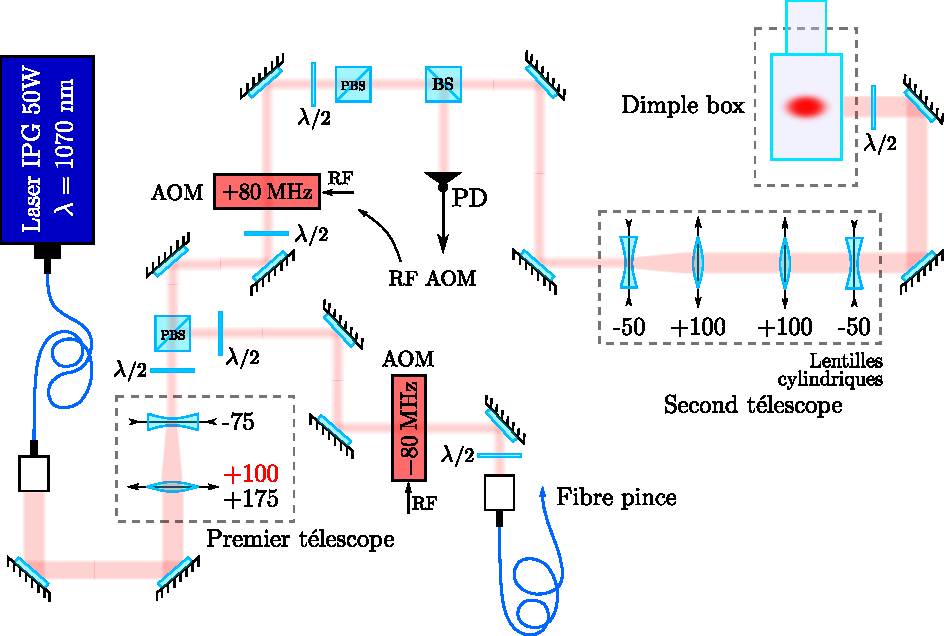
\includegraphics[width=\textwidth]{Fig/Modif_exp/optique_1070_new_style.pdf}
\caption{\textbf{Schéma du montage optique pour le piège dipolaire.} Le faisceau issu du laser source passe dans un premier télescope avant d'être séparé en deux parties. La partie déviée passe dans une fibre optique pour devenir le faisceau de la pince. La partie transmise passe ensuite dans un second télescope pour devenir elliptique et arrive dans la \emph{Dimple box}, qui transmet le faisceau jusqu'aux atomes et contient les optiques d'imagerie \citep{muller2015coherent}. Afin de garder les mêmes tailles de faisceaux, la première lentille du premier télescope, de focale +\SI{175}{\milli\metre}, a été remplacée par une lentille de focale +\SI{100}{\milli\metre}.}
\label{fig:optique_1070}
\end{figure}

Les deux faisceaux du piège dipolaire croisé proviennent d'une source laser commune avant d'être mis en forme séparément. Cette source, un laser fibré Ytterbium de \emph{Keopsys} émettant une puissance initiale de \SI{20}{\watt} en continu à une longueur d'onde $\lambda=\SI{1070}{\nano\metre}$, a été remplacée au cours de ma thèse. Ce laser a été sujet à un grand nombre d'opérations de maintenance, et, dans les mois précédant son changement, il ne pouvait plus émettre que \SI{14}{\watt} lors de son allumage et seulement \SI{12.5}{\watt} en fin de journée.
 
Cette source a été remplacée par un laser fibré Ytterbium \emph{YLR-50-LP-A-Y12} de \emph{IPG}, opérant à la même longueur d'onde $\lambda=\SI{1070}{\nano\metre}$, et avec une puissance maximale mesurée à \SI{55}{\watt}. La taille du faisceau en sortie de fibre est de \SI{0.8}{\milli\metre} (contre \SI{1.4}{\milli\metre} pour le laser Keopsys), il a donc fallu adapter un télescope afin de conserver les mêmes tailles de faisceaux au niveau des atomes. Le montage de mise en forme des faisceaux est présenté figure \ref{fig:optique_1070}. Celui-ci est majoritairement mis dans des tubes (non représentés figure \ref{fig:optique_1070}) contenant un grand nombre de diaphragmes, facilitant ainsi la procédure d'alignement.



\paragraph*{Estimation de la taille du faisceau dimple au niveau des atomes}
L'utilisation d'une fibre optique pour la mise en forme du faisceau de la pince permet de s'assurer que le mode envoyé sur les atomes n'a pas changé. Pour le faisceau dimple en revanche, le trajet jusqu'à la cellule se fait en espace libre. Celui-ci est rendu elliptique à l'aide d'un second télescope, comportant quatre lentilles dont deux cylindriques, comme illustré figure \ref{fig:optique_1070}. Le rapport d'aspect du faisceau est alors de 2. 


%L'approche suivie pour estimer le profil du faisceau au niveau des atomes consiste à en étudier la divergence après la cellule à l'aide d'une caméra, la zone d'intérêt se trouvant sous vide. Un avantage de cette méthode est de s'affranchir d'un système optique qui compliquerait le traitement, sous réserve que la caméra soit suffisamment large pour imager l'entièreté du faisceau. Le principal inconvénient est qu'il est nécessaire d'extrapoler la forme du faisceau pour en estimer le profil au niveau des atomes.

L'estimation de la taille du faisceau au niveau des atomes est réalisée en étudiant l'évolution de son profil d'intensité lumineuse après le passage au travers de la cellule. 
Cette estimation est aisée pour des faisceaux gaussiens: la taille du faisceau $\mathrm{w}_{\mathrm{i}}(y)$ dans la direction $\vec{i}$ ($\vec{i}= \lbrace \vec{x},\vec{z} \rbrace$) est donnée par:
\begin{equation}
\mathrm{w}_{\mathrm{i}}(y)=\mathrm{w}_{\mathrm{i}} \sqrt{1+\left( \frac{y-y_0}{y_{\mathrm{Ri}}} \right)^2} \text{ ,}
\label{eq:taille_faisceau}
\end{equation}
où $y_0$ correspond à la position pour laquelle la taille du faisceau $\mathrm{w}_{\mathrm{i}}(y_0)=\mathrm{w}_{\mathrm{i}}$ est minimale et $\mathrm{w}_{\mathrm{i}}$ est le waist du faisceau. La distance de Rayleigh associée s'exprime $y_{\mathrm{Ri}}=\pi \mathrm{w}_{\mathrm{i}}^2 / \lambda$ et correspond à la distance sur laquelle la taille du faisceau suivant la direction $\vec{i}$ change peu. Dans le régime de champ lointain $y-y_0 \gg y_{\mathrm{Ri}}$, le faisceau diverge selon un angle $\tan \theta_{\mathrm{i}} \simeq \lambda / \pi \mathrm{w}_{\mathrm{i}}$.

La mesure des tailles du faisceau a été réalisée à l'aide d'une caméra \emph{IDS Ueye} disposant d'une matrice de $1024 \times 1280$ pixels de \SI{5.2}{\micro\metre} de côté. Les tailles ont été extraites par ajustement gaussien d'un profil unidimensionnel d'intensité lumineuse obtenu par intégration suivant une direction. Enfin, l'évolution de la taille en fonction de la position a été ajustée par la formule \ref{eq:taille_faisceau}, illustrée figure \ref{fig:taille_dimple}.

\begin{figure}
\centering
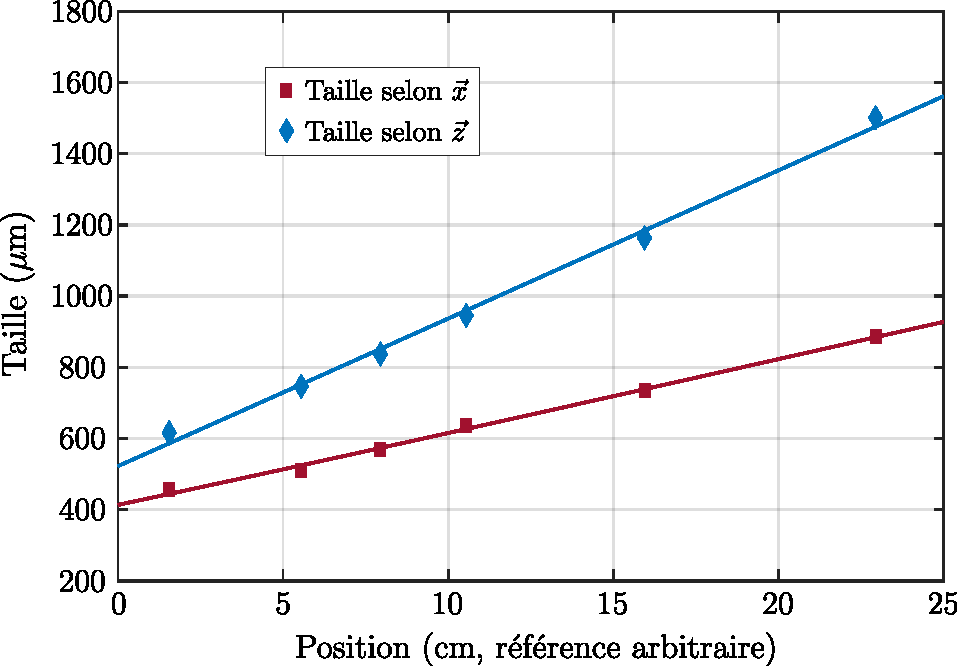
\includegraphics[width=0.7\textwidth]{Fig/Modif_exp/expansion_dimple.pdf}
\caption{\textbf{Évolution des tailles du faisceau dimple après la cellule.} Les tailles du faisceau dimple sont représentées en fonction de la position de la caméra (points). La divergence du faisceau permet de remonter aux waists du faisceau et d'en estimer la position. Les waists extraits par ajustement (lignes continues) sont de $\mathrm{w_z}\simeq \SI{82}{\micro\metre}$ et de $\mathrm{w_x}\simeq \SI{160}{\micro\metre}$ et leur position est compatible avec celle des atomes.}
\label{fig:taille_dimple}
\end{figure}

On estime alors les waists du faisceau dimple à $\mathrm{w_z}=81.6\pm\SI{7.8}{\micro\metre}$ et $\mathrm{w_x}=160\pm \SI{13}{\micro\metre}$, proches des valeurs de la configuration précédant le changement du laser source. La position $y_0$ de ces waists est compatible avec la position des atomes, et la longueur de Rayleigh du faisceau est de l'ordre de $y_{\mathrm{Rz}}\simeq \SI{2}{\centi\metre}$.



\subsection{Calibration du piège optique}
\label{sc:calibration_piege_optique}
%L'utilisation d'une fibre optique pour la mise en forme du faisceau de la pince permet de s'assurer que le mode envoyé sur les atomes n'a pas changé. Pour le faisceau dimple en revanche, le trajet jusqu'à la cellule se fait sans filtrage. La présence de deux périscopes, d'un nombre d'éléments optiques important et l'utilisation d'un profil elliptique imposent une étude attentive des caractéristiques de ce faisceau au niveau des atomes.

La caractérisation finale du piège dipolaire croisé se fait à l'aide des fréquences de piégeage, qui fixent les propriétés physiques du nuage. %Afin de mesurer ces fréquences, nous avons fait le choix d'induire de petites oscillations du nuage à l'intérieur du piège à l'aide d'une force extérieure, et de suivre ces oscillations en fonction du temps d'évolution dans le piège de manière équivalente à celle présentée pour la lévitation magnétique section \ref{sc:oscillations_levitation}. 


\paragraph*{Calibration des fréquences de piégeage}
Le fonctionnement du piège optique repose sur le potentiel dipolaire. Celui-ci s'écrit:
\begin{equation}
U(\mathbf{r})=\frac{3 \pi c^2 \Gamma}{2 \omega_0^3 \overline{\Delta}} I(\mathbf{r}) \quad \text{avec} \quad \frac{1}{\overline{\Delta}}=\frac{1}{\omega-\omega_0}-\frac{1}{\omega+\omega_0} \text{ .}
\end{equation}
Les faisceaux utilisés étant de forme gaussienne, on peut ainsi exprimer la profondeur de piégeage de chaque faisceau:
\begin{equation}
U_{\mathrm{pince}}= \frac{3c^2 \Gamma }{\omega_0^3 \overline{\Delta}} \frac{P_{\mathrm{pince}}}{\mathrm{w}_0^2} \quad \text{et} \quad U_{\mathrm{dimple}}=\frac{3c^2 \Gamma }{\omega_0^3 \overline{\Delta}}\frac{P_{\mathrm{dimple}}}{\mathrm{w}_{\mathrm{x}} \mathrm{w}_{\mathrm{z}}} \text{ .}
\label{eq:profondeur_piege_optique}
\end{equation}
En supposant que les atomes restent proches du centre du piège, on peut de plus faire l'approximation que le profil d'intensité des faisceaux est de forme harmonique. On définit ainsi les fréquences de piégeage $\omega_{x,y,z}$ par analogie avec un oscillateur harmonique. Rappelons que le confinement dans les directions $\vec{x}$ et $\vec{y}$ est fait par la pince, et que celui dans la direction $\vec{z}$ est fait par le dimple, les fréquences de piégeage du piège dipolaire croisé s'expriment alors:
\begin{equation}
\omega_x=\omega_y=\sqrt{-\frac{4 U_{\mathrm{pince}}}{m \mathrm{w}_0^2}} \quad \text{et} \quad \omega_z=\sqrt{-\frac{4U_{\mathrm{dimple}}}{m \mathrm{w}_{\mathrm{z}}^2}} \text{ .}
\label{eq:frequences_piege_optique}
\end{equation}
%La caractérisation finale du piège dipolaire croisé se fait à l'aide des fréquences de piégeage, qui fixent les propriétés physiques du nuage. 
Afin de mesurer ces fréquences, nous avons fait le choix\footnote{Nous avons retenu la méthode de mesure des fréquences de piégeage à l'aide d'excitations dipolaires. Il est aussi possible de mesurer ces fréquences par excitations paramétriques à l'aide de petites modulations de la profondeur du piège \citep{savard1997laser}.} d'induire de petites oscillations du centre de masse du nuage à l'intérieur du piège à l'aide d'une force extérieure, et de suivre ces oscillations en fonction du temps d'évolution dans le piège de manière équivalente à celle présentée pour la lévitation magnétique section \ref{sc:oscillations_levitation}. En relevant la position des atomes en fonction de la durée d'évolution dans le piège après excitation, on extrait alors la fréquence associée à l'aide d'un ajustement illustré figure \ref{fig:frequences_piege_optique}.a.

La fréquence de piégeage dans les directions $\vec{x}$ et $\vec{y}$, liée à la pince optique, a pu être mesurée à l'aide de la lévitation magnétique. En commutant rapidement le courant des bobines de gradient, on dispose d'un bouton pour allumer et éteindre la gravité, et donc générer une force pendant un bref instant pour donner un mouvement aux atomes dans le piège. La mesure de la fréquence de piégeage dans la direction $\vec{z}$ a été effectuée selon deux méthodes en fonction de la puissance du faisceau dimple:
\begin{itemize}
\item[\textendash] À haute puissance, les atomes sont poussés à l'aide d'un gradient magnétique suivant la direction $\vec{z}$ provenant de bobines de compensation branchées en configuration anti-Helmholtz. Celles-ci peuvent exercer une force sur les atomes pendant de courts instants à l'aide d'un commutateur rapide.
\item[\textendash] À plus basse puissance, le piège optique est très décomprimé et peu profond. Cependant, le piégeage de la lévitation peut arracher les atomes du piège optique, il est donc nécessaire de déplacer le centre de la lévitation magnétique à l'aide de champs de compensation suivant la direction $\vec{z}$. Pour pousser les atomes, on utilise alors les bobines de compensation dans leur configuration normale, et leur brève extinction conduit à accélérer les atomes en déplaçant le centre de la lévitation magnétique.
\end{itemize}

\begin{figure}
\centering
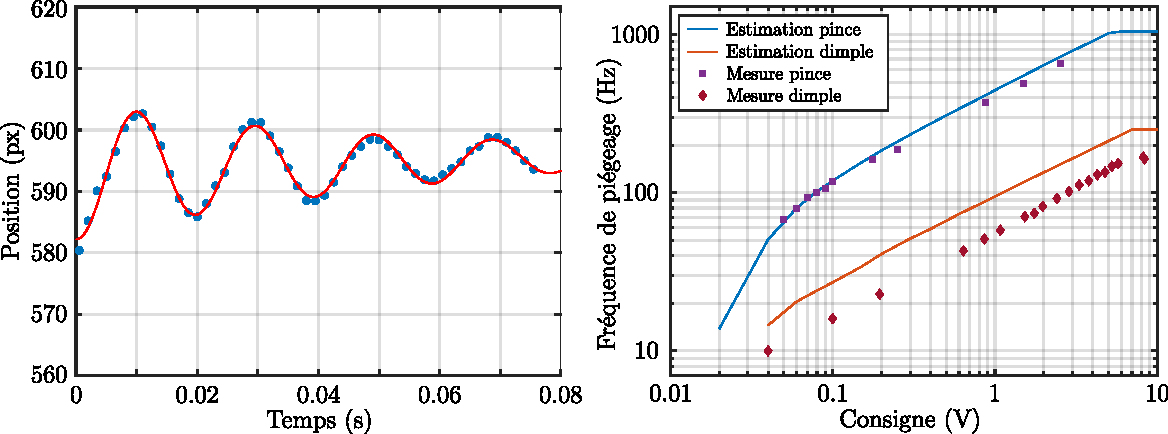
\includegraphics[width=\textwidth]{Fig/Modif_exp/frequences_piege_optique.pdf}
\caption{\textbf{a: Exemple d'oscillation dans le piège optique.} Le nuage oscille dans la direction $\vec{z}$ pour une puissance du faisceau dimple de \SI{0.70}{\watt} après avoir été poussé par un gradient magnétique (points bleus). La fréquence d'oscillation est alors de $\omega_z /2\pi \simeq \SI{51}{\hertz}$, extraite par ajustement (courbe noire). \textbf{b: Fréquences d'oscillations du piège optique.} Les fréquences mesurées par oscillations du nuage (points) sont tracées en fonction de la puissance du faisceau associé. Les valeurs des calibrations $A_{\mathrm{pince}}$ et $A_{\mathrm{dimple}}$ sont ensuite extraites par ajustement de ces données (lignes continues).}
\label{fig:frequences_piege_optique}
\end{figure}

L'évolution des fréquences de piégeage de chaque faisceau en fonction de la puissance optique est représentée figure \ref{fig:frequences_piege_optique}.b en échelle logarithmique. La variation des fréquences s'est faite en abaissant la puissance du laser au cours de l'évaporation optique, celle-ci conduisant à une décompression du piège de comportement $\omega /2\pi =A \sqrt{P}$ comme le témoignent les formules \ref{eq:profondeur_piege_optique} et \ref{eq:frequences_piege_optique}. Les fréquences mesurées expérimentalement (carrés pour la pince optique, losanges pour le faisceau dimple) sont ajustées par une loi de puissance (lignes continues). La calibration de la pince est alors déterminée à $A_{\mathrm{pince}}=980\pm \SI{20}{\hertz\per\watt^{1/2}}$, et celle du dimple à $A_{\mathrm{dimple}}=60.5\pm \SI{1.0}{\hertz\per\watt^{1/2}}$, proche de la valeur précédant le remplacement du laser source\footnote{La dernière calibration date de la mise en place de la \emph{dimple box} lors de la thèse de Kilian Muller \citep{muller2015coherent}. Celle du dimple était alors de $A_{\mathrm{dimple}}=64.5\pm \SI{1.2}{\hertz\per\watt^{1/2}}$.}.







%Une seconde conséquence de la figure \ref{fig:frequences_piege_optique} est que les deux faisceaux présentent une saturation à haute puissance, c'est à dire qu'ils restent à leur puissance maximale au delà d'une certaine consigne seuil. Pour le dimple, cette saturation provient d'une limitation de la puissance de la source de la radio-fréquence servant à la diffraction du faisceau dans le modulateur acousto-optique. Pour la pince, cette limitation provient du maximum de l'efficacité de diffraction du modulateur acousto-optique. Ces deux saturations peuvent être repoussées en augmentant la puissance émise par le laser source\footnote{Le réglage actuellement utilisé sur l'expérience est une émission à 50\% de la puissance maximale du laser \emph{IPG}, c'est à dire environ \SI{23}{\watt}. Il a été observé que le mode émis est suffisamment stable à ce point de fonctionnement.}, cependant elles ne sont pas problématiques pour notre configuration. De plus, cette augmentation de puissance se traduirait par un chauffage local des bloqueurs de faisceau plus important, entraînant des effets thermiques néfastes.












\section{Optimisation de l'évaporation tout-optique}
\label{sc:evap_optique}
Vingt-cinq ans après l'obtention du premier condensat de Bose-Einstein, l'étape de refroidissement par évaporation forcée reste un passage obligatoire pour l'obtention d'un gaz dégénéré, à l'exception de quelques développements récents se basant sur des techniques novatrices de refroidissement laser \citep{stellmer2013laser} \citep{hu2017creation}. 

Comme brièvement présenté dans le chapitre précédent, le principe du refroidissement évaporatif repose sur l'extraction de particules très énergétiques, suivie par la thermalisation des particules restantes moins énergétiques en moyenne, se traduisant donc par une diminution de la température. Néanmoins, l'efficacité de ce processus dépend fortement de la configuration expérimentale. Les modifications apportées à notre piège optique nécessitent donc d'adapter les consignes d'évaporation à notre nouvelle géométrie. %De plus, l'utilisation de nouvelles cartes analogiques \emph{National Instruments} avec la suite \emph{Cicero Word Generator} permet de générer de nouvelles consignes arbitraires, non limitées à des morceaux de rampes telles qu'auparavant. 

Dans cette partie, nous commencerons par présenter le fonctionnement du refroidissement par évaporation forcée, puis nous détaillerons les résultats de l'optimisation de notre évaporation optique dans un second temps.


\subsection{Lois d'échelle du refroidissement évaporatif}
\label{sc:scaling_laws_ohara}
Le but de l'étape de refroidissement évaporatif étant d'augmenter la densité dans l'espace des phases $\mathcal{D}=n \ldb^3$, aussi appelée \emph{paramètre de dégénérescence}, il est donc nécessaire que notre système présente de la dissipation afin de franchir le seuil de condensation \citep{metcalf2007laser}. L'origine de cette dissipation repose sur la profondeur finie des pièges utilisés.  

\paragraph*{Évaporation naturelle dans un piège de profondeur finie}
Une conséquence de cette profondeur finie est que la fonction de partition $f(E)$ est tronquée à l'énergie $U$ correspondant à la profondeur du piège. Plus précisément, il a été montré que la fonction de partition est très proche d'une distribution de Boltzmann tronquée \citep{luiten1996kinetic}:
\begin{equation}
f(E)\propto e^{-\frac{E}{\kB T}} \Theta(U-E) \text{ .}
\label{eq:fonction_partition}
\end{equation}
Le temps de convergence vers cette distribution, c'est à dire le temps de thermalisation $\tau_{\mathrm{th}}$, est de l'ordre de quelques collisions entres les particules du gaz, dont le taux s'exprime $\Gamma_{\mathrm{c}}=n \sigma \overline{v}$, avec $n$ la densité du gaz, $\sigma$ la section efficace de diffusion et $\overline{v}$ la vitesse moyenne relative entre deux atomes \citep{walraven2010elements}.

En effet, la collision de deux particules permet de transférer de l'énergie d'une particule à la seconde. En particulier, une particule est susceptible d'acquérir par collision une énergie mécanique totale supérieure à la profondeur de piège, celle-ci est donc extraite du piège et emporte une énergie $U+\kappa\kB T$ ($\kappa>0$) supérieure à l'énergie moyenne par particule. %La particule restante a quant à elle perdu de l'énergie. 

Ce processus étant le plus probable pour des particules de grandes énergies, celui-ci favorise l'accumulation des particules dans les états de basse énergie tandis qu'il dépeuple les états de grande énergie. Ce raisonnement permet d'expliquer de manière qualitative la forme de la fonction de partition \ref{eq:fonction_partition}, qui favorise les états de basse énergie.

Ce phénomène d'\emph{évaporation naturelle} conduit donc à une diminution de la température, dont l'efficacité décroît avec le refroidissement du nuage. En effet, l'énergie moyenne par particule diminuant, la probabilité que des particules acquièrent suffisamment d'énergie pour s'échapper du piège décroît exponentiellement \citep{walraven2010elements}. Ainsi, le processus d'évaporation naturelle est fortement ralenti et le taux d'évaporation, c'est à dire le nombre de particules expulsées du piège par évaporation naturelle par unité de temps, peut être estimé par 
\begin{equation}
\Gamma_{\mathrm{ev}}\sim e^{-U/\kB T} \Gamma_{\mathrm{c}} \text{ ,}
\label{eq:taux_evap}
\end{equation}
avec $\Gamma_{\mathrm{c}}$ le taux de collisions. Le taux d'évaporation devient ainsi exponentiellement petit, l'évaporation est alors figée. 	

%Très rapidement, le temps d'évaporation $1/\Gamma_{\mathrm{ev}}$ excède le temps de vie des atomes dans le piège et ceux-ci sont perdus par des collisions inélastiques. 
Afin de dépasser cette limitation et de garder une évaporation efficace, la technique expérimentale développée afin d'obtenir les premiers condensats de Bose-Einstein consiste à abaisser progressivement la profondeur du piège $U$. On parle alors d'\emph{évaporation forcée}.





\paragraph*{Lois d'échelle de l'évaporation forcée}
Comme mentionné précédemment, la mise en œuvre pratique du refroidissement évaporatif se fait par le biais de la diminution de la profondeur du piège, forçant ainsi le processus d'évaporation. Cette opération est réalisée en continu, et à une vitesse suffisamment lente devant le temps de thermalisation $\tau_{\mathrm{th}}$ afin que le système soit constamment à l'équilibre thermodynamique\footnote{Dans ce cas, les seules pertes d'atomes considérées sont celles liées à l'évaporation par collisions. Cela revient à négliger la dynamique de thermalisation de l'évaporation, qui fait apparaître les pertes par déversement\citep{cohen1996atomes}. Celles-ci correspondent aux atomes ayant une énergie de $U-\delta E$ qui ne sont plus piégés lors de l'abaissement de la profondeur du piège de $U$ à $U-\mathrm{d}U$, avec $\mathrm{d}U > \delta E$. Dans le cas d'un gaz à l'équilibre thermodynamique, seule une infime partie des atomes se trouve dans cet intervalle d'énergie que l'on peut négliger devant les autres sources de pertes.}. 


On pressent à l'aide de l'équation \ref{eq:taux_evap} que le rapport entre la profondeur du piège et la température du gaz piégé joue un rôle fondamental dans l'évaporation. On définit alors le paramètre de troncature $\eta$:
\begin{equation}
\eta=\frac{U}{\kB T} \text{ .}
\end{equation}
Dans le cas d'un abaissement lent et continu de la profondeur du piège, le paramètre de troncature est approximativement constant\footnote{Étant donné la dépendance exponentielle du taux d'évaporation en $\eta$, le processus d'évaporation sera très fortement ralenti dans le cas d'un nuage très froid ($\eta$ grand), et rapide dans le cas d'un nuage chaud ($\eta$ petit). Lors de l'abaissement progressif de la profondeur du piège, la température va donc varier avec la profondeur du piège.} et sa valeur est de l'ordre de $\eta\approx 10$ dans le cas d'un piège optique.



Le potentiel de piégeage $U(\mathbf{x},t)$ étant modifié au cours de l'évaporation, les atomes sont soumis à un potentiel variant dans le temps. Dans le cas d'un piège harmonique, les fréquences de piégeage associées peuvent changer au cours de l'évaporation en fonction de l'implémentation expérimentale du refroidissement évaporatif. %\footnote{La méthode de couteau radio-fréquence utilisée dans le piège magnétique dans la première chambre ne modifie pas les fréquences de piégeages et ne change que la profondeur du piège, tandis que l'évaporation tout optique, réalisée à l'aide de faisceaux lasers de tailles fixées, est accompagnée d'une décompression du piège lors de l'abaissement de la puissance des lasers.}
Les variations de la géométrie du piège sont alors caractérisées par le paramètre $\nu$ défini par
\begin{equation}
\nu=\frac{\dot{\overline{\omega}}/\overline{\omega}}{\dot{U}/U}
\end{equation}
où $\overline{\omega}$ est la moyenne géométrique des fréquences du piège. Comme explicité formule \ref{eq:frequences_piege_optique}, les fréquences de piégeage du piège optique évoluent en $\overline{\omega}\propto\sqrt{U}$, impliquant donc $\nu=0.5$ \citep{o2001scaling}. L'abaissement de la profondeur du piège sera donc forcément accompagnée d'une décompression de celui-ci. 




Dressons alors un bilan d'énergie afin de déterminer la manière dont varient les principales quantités thermodynamiques au cours de l'évaporation. L'énergie totale du gaz dans un piège harmonique est donnée par
\begin{equation}
E=3N\kB T
\end{equation}
avec $N$ le nombre total d'atomes. La variation temporelle de l'énergie totale du gaz est alors donnée par
\begin{equation}
\dot{E}=3\dot{N} \kB T + 3 N \kB \dot{T} \text{ ,}
\label{eq:variation_energie_derivee}
\end{equation}
exprimée en fonction des variations temporelles du nombre d'atomes et de la température.

En identifiant les différentes sources de variations de l'énergie totale, on montre que la variation de l'énergie totale du système est donnée par \citep{cohen1996atomes}
\begin{equation}
\dot{E}=\dot{N}(U+\kappa \kB T) +\nu\frac{\dot{U}}{U}E \text{ ,}
\label{eq:variation_energie_bilan}
\end{equation}
où le premier terme décrit la perte d'énergie liée à l'évaporation des atomes énergétiques et le second terme représente le changement d'énergie potentielle des particules restées dans le piège, traduisant la décompression de ce dernier. Dans le cas d'une évaporation 3D, $\kappa=3/2$ \citep{ketterle1996evaporative}.

En combinant les équations \ref{eq:variation_energie_derivee} et \ref{eq:variation_energie_bilan}, on montre alors que la variation du nombre d'atomes en fonction de la profondeur de piégeage est donnée par \citep{o2001scaling}:
\begin{equation}
\frac{\dot{N}}{N}={\frac{3(1-\nu)}{\eta'-3}} \frac{\dot{U}}{U} \text{ ,}
\label{eq:nombre_atome_evap}
\end{equation}
avec $\eta'=\eta+\kappa$. Il est alors possible de déterminer les lois d'échelle des différentes grandeurs thermodynamiques d'un gaz classique. 

En particulier, dans le cas d'un piège harmonique, la densité dans l'espace des phases s'exprime:
\begin{equation}
\mathcal{D}=N\left(\frac{\hb \overline{\omega}}{\kB T}\right)^3 \text{ .}
\end{equation}
On peut alors déterminer les variations du paramètre de dégénérescence en fonction des variations du nombre d'atomes: 
\begin{equation}
\frac{\dot{\mathcal{D}}}{\mathcal{D}} = -\gamma \frac{\dot{N}}{N} \text{ .}
\label{eq:efficacite_evaporation}
\end{equation}
Le paramètre $\gamma=\eta'-4$ correspond à l'efficacité du processus d'évaporation: la perte d'atomes engendre un gain de densité dans l'espace des phases d'autant plus élevé que ce paramètre est grand. L'enjeu de l'optimisation du refroidissement évaporatif consiste donc à augmenter cette efficacité autant que possible.

Une conséquence remarquable de l'équation \ref{eq:efficacite_evaporation} est que l'efficacité du processus d'évaporation ne dépend pas du paramètre $\nu$ témoignant du changement de forme du piège. Ceci s'explique par le fait que pour une évaporation à $\eta$ constant, le paramètre $\nu$ traduit une ouverture adiabatique du piège, la décompression du nuage étant accompagnée d'une diminution de la température, voir section \ref{sc:chambre_science}. 


\paragraph*{Taux de collisions et régime d'emballement}
Si l'équation \ref{eq:efficacite_evaporation} ne fait pas apparaître l'influence du paramètre $\nu$, celui-ci joue cependant un rôle primordial quant à la cinétique de l'évaporation. En effet, la vitesse maximale d'évaporation est limitée par la vitesse à laquelle le gaz atteint un état d'équilibre thermique, c'est à dire le taux de thermalisation $1/\tau_{\mathrm{th}}$. Celui-ci est de l'ordre du taux de collisions $\Gamma_{\mathrm{c}}$, qui varie au cours de l'évaporation avec le nombre d'atomes, la température et la forme du piège.%=n \sigma \overline{v}$, avec $n$ la densité du gaz, $\sigma$ la section efficace de diffusion et $\overline{v}$ la vitesse moyenne relative entre deux atomes \citep{walraven2010elements}. 

Dans le cas d'un piège harmonique, on montre que la loi de variation du taux de collisions peut s'écrire \citep{o2001scaling}
\begin{equation}
\frac{\dot{\Gamma}_{\mathrm{c}}}{\Gamma_{\mathrm{c}}}=\left[ 1- (\eta'-3) \left( \frac{1-3\nu}{3(1-\nu)}\right)\right] \frac{\dot{N}}{N} \text{ ,}
\end{equation}
où le facteur entre crochets peut changer de signe suivant la valeur de $\nu$. Ainsi, il est possible que le taux de collisions augmente au cours de l'évaporation malgré la perte d'atomes, rendant ainsi l'évaporation de plus en plus rapide. Dans ce régime d'\emph{emballement}, la diminution du nombre d'atomes et de leur vitesse relative moyenne est plus que compensée par une forte augmentation de la densité au centre du piège, augmentant ainsi le taux de collisions. Ce régime peut être atteint pour de faibles valeurs de $\nu$, en particulier pour l'évaporation radio-fréquence dans notre piège magnétique où $\nu=0$. 

En revanche, l'évaporation optique est réalisée en abaissant la puissance des faisceaux laser dont la taille est gardée fixe, processus pour lequel $\nu=0.5$. Dans ce régime, le taux de collisions diminue au cours de l'évaporation, la rendant de plus en plus lente contrairement au régime d'emballement. Il est donc primordial qu'une évaporation optique commence avec un grand taux de collisions pour permettre une thermalisation rapide. De manière générale, une évaporation optique possède une première phase pendant laquelle la puissance des faisceaux laser est abaissée rapidement, la thermalisation du nuage étant immédiate grâce au grand taux initial de collisions, puis une seconde phase plus lente où la thermalisation du nuage nécessite plus de temps. 


\paragraph*{Consigne d'évaporation}
Les lois d'échelle présentées dans la section précédente montrent comment évoluent les différentes grandeurs thermodynamiques du nuage en fonction de la profondeur du piège, sans pour autant spécifier la dépendance temporelle de celle-ci. Afin de déterminer le profil optimal de la consigne d'évaporation, il est possible d'établir un bilan du nombre d'atomes présents dans le piège\footnote{Les lois d'échelle présentées dans les paragraphes précédents ont été obtenues à l'aide d'un bilan d'énergie.}.
En considérant que les atomes sont uniquement perdus par évaporation, on peut écrire les variations du nombre d'atomes à l'aide d'une équation de taux \citep{luiten1996kinetic}\citep{o2001scaling}
\begin{equation}
\dot{N} = - \Gamma_{\mathrm{ev}} N \quad \text{avec} \quad \Gamma_{\mathrm{ev}}=2(\eta-4) e^{-\eta} \Gamma_{\mathrm{c}} \text{ .}
\label{eq:pertes_evap_naturelle}
\end{equation}

On peut alors déterminer que le profil optimal de la consigne d'évaporation est aussi donné par une loi de puissance \citep{o2001scaling}:
\begin{equation}
U(t)=U_{\mathrm{0}} {\left( 1+\frac{t}{\tau}\right) }^{-\beta} \text{ ,}
\label{eq:nouvelle_consigne_evap}
\end{equation}
avec $U_{\mathrm{0}}=U(t=0)$ la profondeur initiale du piège au début de l'étape d'évaporation. Les paramètres $\tau$ et $\beta$ dépendent du paramètre de troncature $\eta$, de la géométrie du piège et du taux de collisions initial $\Gamma_{\mathrm{c}}(t=0)$.

On remarque que la consigne d'évaporation \ref{eq:nouvelle_consigne_evap} possède deux dynamiques distinctes. Comme annoncé dans le paragraphe précédent, l'évaporation est dans un premier temps rapide afin de profiter du grand taux de collisions, puis dans un second temps, la consigne est lentement abaissée en raison de l'augmentation du temps de thermalisation. 
 


\paragraph*{Effet des collisions inélastiques}
En pratique, l'évaporation par collisions n'est pas la seule source de perte des particules. L'expérience se déroulant à l'intérieur d'une enceinte sous ultra-vide pompée en continu, les collisions avec les particules du gaz résiduel à température ambiante sont responsables de pertes indépendantes de l'énergie des atomes piégés. Cela se traduit par un temps de vie $1/\Gamma_{\mathrm{bg}}$ fini des atomes dans le piège.

On peut alors écrire les pertes d'atomes liées au gaz résiduel sous la forme d'équations de taux
\begin{align}
\dot{N}_{\mathrm{bg}}&=-\Gamma_{\mathrm{bg}} N  \\
\dot{E}_{\mathrm{bg}}&=-\Gamma_{\mathrm{bg}} E \text{ ,}
\end{align}
où le temps de vie $1/\Gamma_{\mathrm{bg}}$ est de l'ordre de \SI{10}{\second}. 

Deux régimes limites se présentent alors. Dans le cas d'une évaporation rapide telle que $\Gamma_{\mathrm{ev}} \gg \Gamma_{\mathrm{bg}}$, l'essentiel des pertes d'atomes est dû au processus d'évaporation. La présence du gaz résiduel n'a donc que peu d'effet sur le nuage, l'évaporation pouvant se dérouler sur une durée petite devant le temps de vie des atomes dans le piège. 

Au contraire, les pertes dues au gaz résiduel peuvent fortement entraver le processus d'évaporation dans le cas d'un petit temps de vie, dans le régime où $\Gamma_{\mathrm{ev}} \ll \Gamma_{\mathrm{bg}}$. Dans ces conditions, les atomes ne peuvent rester assez longtemps dans le piège pour que certains aient le temps d'acquérir une énergie suffisante pour être évaporés.



Les collisions avec le gaz résiduel ne sont pas la seule source néfaste de perte d'atomes. Des processus complexes liés à la nature métastable des expériences d'atomes froids peuvent conduire à la perte de plusieurs atomes. Aux températures atteintes par les nuages piégés, la majorité des éléments devraient se trouver à l'état solide, mais le caractère élastique des collisions binaires permet au système de rester sous forme gazeuse. Cependant, il est possible que lors d'une collision tertiaire, deux atomes établissent une liaison moléculaire, dont la grande énergie est évacuée par le biais d'un troisième atome. Ce processus de pertes à trois corps conduit alors à la perte des trois atomes. 

Puisque ce mécanisme nécessite la collision de trois atomes, on peut décrire la variation de densité due aux pertes à trois corps ainsi que la variation de l'énergie totale à l'aide d'une loi de puissance:
\begin{align}
\dot{n}_{\mathrm{3b}}(\mathbf{x})&=-K_{\mathrm{3b}} n^3(\mathbf{x}) \label{eq:pertes_atomes_3corps} \\
\dot{E}_{\mathrm{3b}}&= \frac{3}{2}\dot{N}_{\mathrm{3b}} \kB T + \int{\mathrm{d}\mathbf{x} \: U(\mathbf{x}) \dot{n}_{\mathrm{3b}}(\mathbf{x})}\text{ ,}
\end{align}
où le coefficient $K_{\mathrm{3b}}$ est une constante du \isotope[87]{Rb} et vaut \SI{1.8e-29}{\centi\metre^6\second^{-1}} \citep{burt1997coherence}\citep{soding1999three}.


Comme illustré par l'équation \ref{eq:pertes_atomes_3corps}, le mécanisme de pertes à trois corps devient important dans des régions de fortes densités. Les pièges optiques étant fortement comprimés afin d'avoir un taux de collisions suffisant pour pouvoir évaporer, ceux-ci sont particulièrement susceptibles de générer des pertes à trois corps. 

En présence de ces pertes, il est possible de modifier les lois d'échelles présentées précédemment \citep{luiten1996kinetic}\citep{brantut2009manipulation}. En particulier, on peut montrer que dans le cas d'un piège harmonique profond, l'équation \ref{eq:nombre_atome_evap} régissant l'évolution du nombre d'atomes se généralise en
\begin{equation}
\frac{\dot{N}}{N}= \left( \frac{\eta'-3}{3(1-\nu)} + R \frac{2-\eta'}{3(1-\nu)} \right)^{-1} \frac{\dot{U}}{U} \text{ ,}
\label{eq:scaling_atomes_3corps}
\end{equation}
où la quantité $R=\dot{N}_{\mathrm{3b}}/\dot{N}$ est la fraction d'atomes perdus par collisions à trois corps. De même, l'équation \ref{eq:efficacite_evaporation} devient
\begin{equation}
\frac{\dot{\mathcal{D}}}{\mathcal{D}}=-\gamma \frac{\dot{N}}{N} \quad \text{avec} \quad \gamma=\eta'-4 + R(2-\eta') \text{ ,}
\label{eq:efficacite_evap_3corps}
\end{equation}
témoignant ainsi de la réduction de l'efficacité de l'évaporation par les pertes à trois corps.





\subsection{Résultats de l'optimisation de l'évaporation}
Nous allons à présent détailler la manière dont cette étape d'évaporation est implémentée sur notre dispositif. Les résultats présentés ici sont le fruit d'une optimisation de l'efficacité de l'évaporation, où nous avons maximisé le gain de densité dans l'espace des phases vis-à-vis de la perte d'atomes. %De plus, nous discuterons l'influence qu'a la lévitation magnétique lors de cette étape de refroidissement.



\paragraph*{Consigne d'évaporation}
L'implémentation de la formule \ref{eq:nouvelle_consigne_evap} comme consigne de puissance\footnote{La pesanteur a pour effet de \textit{pencher} le potentiel, pouvant changer la dimensionnalité de l'évaporation \citep{boyer2000condensation}, mais aussi limiter la profondeur du piège optique à environ $U/\kB \sim \SI{2.5}{\micro\kelvin}$ pour laquelle la gradient maximal d'intensité lumineuse ne permet plus de compenser le poids des atomes. L'utilisation de la lévitation magnétique au cours de l'évaporation permet alors de dépasser cette limitation, et de rendre la profondeur du piège directement donnée par la puissance des faisceaux en s'affranchissant de la gravité. } sur les deux faisceaux du piège dipolaire est rendue possible grâce à l'utilisation des nouvelles cartes analogiques \emph{National Instruments} et de la suite \emph{Cicero Word Generator}.
L'optimisation de l'étape d'évaporation nous a permis de déterminer les paramètres $\beta_{\mathrm{pince}}=\beta_{\mathrm{dimple}}=6$, $\tau_{\mathrm{pince}}=\SI{1.2}{\second}$ et $\tau_{\mathrm{dimple}}=\SI{1.3}{\second}$. La nouvelle consigne d'évaporation est alors tracée figure \ref{fig:comparaison_consigne_evap}, et est comparée à la consigne composée de morceaux de rampes linéaires\footnote{Les cartes analogiques du précédent système informatique de contrôle de l'expérience ne permettait d'utiliser que des profils de consignes composées de morceaux de rampes linéaires. } de notre configuration précédente.

\begin{figure}
\centering
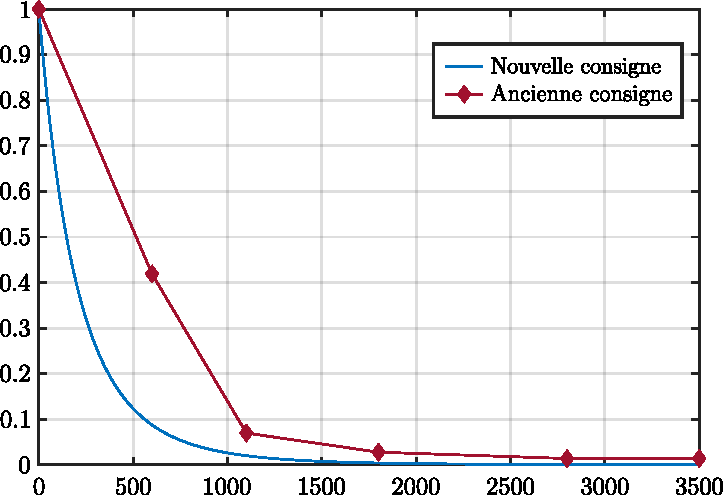
\includegraphics[width=0.7\textwidth]{Fig/Modif_exp/comparaison_consignes_evap.pdf}
\caption{\textbf{Comparaison de la nouvelle et de l'ancienne consigne d'évaporation du faisceau pince.} L'ancienne consigne, composée de cinq morceaux de rampe linéaire, est représentée en bordeaux. La nouvelle consigne, donnée par l'équation \ref{eq:nouvelle_consigne_evap} est représentée en bleu, possède une décroissance plus rapide que dans le cas de l'ancienne consigne. Elle permet de plus d'obtenir un condensat de Bose-Einstein plus rapidement.}
\label{fig:comparaison_consigne_evap}
\end{figure}

Par construction, la formule \ref{eq:nouvelle_consigne_evap} permet de mieux tirer parti du processus d'évaporation naturelle. Il est alors possible d'effectuer une évaporation plus rapide, réduisant l'impact de la durée de vie finie des atomes par collisions avec le gaz résiduel. 

Dans la suite, nous nous concentrerons sur les premières \SI{700}{\milli\second} de l'évaporation, qui correspondent à la durée nécessaire pour atteindre le seuil $\mathcal{D}\approx 1$, pour lequel une partie condensée apparaît. Au delà de ce seuil, l'approche classique pour laquelle les lois d'échelle ont été déterminées précédemment n'est plus valide.%\footnote{Dans le cadre d'une évaporation à $\eta$ constant, le taux de pertes à trois corps ne dépend pas de la vitesse à laquelle l'évaporation est effectuée.}.
 



\paragraph*{Évolution de la température}

L'évolution de la température du nuage\footnote{La détermination expérimentale de la température en présence du champ de lévitation, basée sur le principe de focalisation atomique, est détaillée dans l'annexe \ref{ch:anex_mesure_temp}.} au cours de l'évaporation est représentée figure \ref{fig:eta_constant}, et témoigne d'un refroidissement important au cours de l'évaporation, comme attendu. Nous avons superposé à ces mesures la profondeur estimée\footnote{Cette estimation provient de la calibration du piège optique présentée section \ref{sc:calibration_piege_optique}.} de la pince divisée par 10, sans paramètre ajustable. L'accord entre ces courbes est remarquable, validant ainsi l'approche d'une évaporation à $\eta=10$ constant. Ceci constitue une preuve du caractère adiabatique de notre évaporation, le nuage étant constamment dans un état de quasi-équilibre thermodynamique.

\begin{figure}
\centering
\includegraphics[width=0.7\textwidth]{Fig/Modif_exp/Evolution_température_eta.pdf}
\caption{\textbf{Évolution de la température au cours de l'évaporation.} La température (points bleus) est mesurée après différentes durées d'évaporation et comparée à la profondeur de piégeage du faisceau pince divisée par 10 (courbe noire). Sans paramètre ajustable, les deux courbes se superposent remarquablement.}
\label{fig:eta_constant}
\end{figure}







\paragraph*{Évolution du nombre d'atomes}

L'évolution du nombre d'atomes au cours de l'évaporation présente un intérêt particulier car celle-ci contient les informations liées aux processus de pertes inélastiques. Notamment, nous pouvons estimer le taux de pertes à trois corps à l'aide d'une mesure de la densité atomique et de la formule \ref{eq:pertes_atomes_3corps}. En comparant ces pertes aux variations mesurées du nombre d'atomes, on détermine que le rapport $R=\dot{N}_{\mathrm{3b}}/\dot{N}$ de l'ordre de 0.1, approximativement constant tout au long de l'évaporation. Il apparaît donc que les pertes à trois corps ont un effet marqué sur l'évolution du nombre d'atomes au cours de l'évaporation, mais que celles-ci ne constituent pas une limite pour notre système. 

De plus, il est possible de négliger l'effet des pertes dues aux collisions avec le gaz résiduel, limitant le temps de vie des atomes dans le piège à $1/\Gamma_{\mathrm{bg}}\approx\SI{10}{\second}$. En effet, l'optimisation de notre évaporation se concentre sur les premières \SI{700}{\milli\second} d'abaissement de la profondeur du piège\footnote{Cette durée correspond au temps nécessaire pour franchir le seuil de condensation $\mathcal{D}\approx 1$ et l'obtention d'un gaz dégénéré. Celle-ci était d'environ \SI{1.2}{\second} avec l'ancienne consigne.} comme illustré sur les figures \ref{fig:eta_constant} et \ref{fig:nombre_atomes_evap}, et la durée totale de notre évaporation est de \SI{3.5}{\second}, courte comparée au temps de vie permis par le gaz résiduel.

L'évolution du nombre d'atomes au cours de l'évaporation est représentée figure \ref{fig:nombre_atomes_evap} et est comparée à la prédiction de la loi d'échelle \ref{eq:scaling_atomes_3corps}, tracée avec les paramètres $\eta=10$ (déterminé précédemment grâce à l'évolution de la température au cours de l'évaporation) et $R=0.1$ (déterminé en estimant le taux de pertes à trois corps et rapporté aux pertes totales mesurées expérimentalement). Il apparaît donc que la théorie d'échelle permet de décrire correctement l'évolution du nombre d'atomes. 


\begin{figure}
\centering
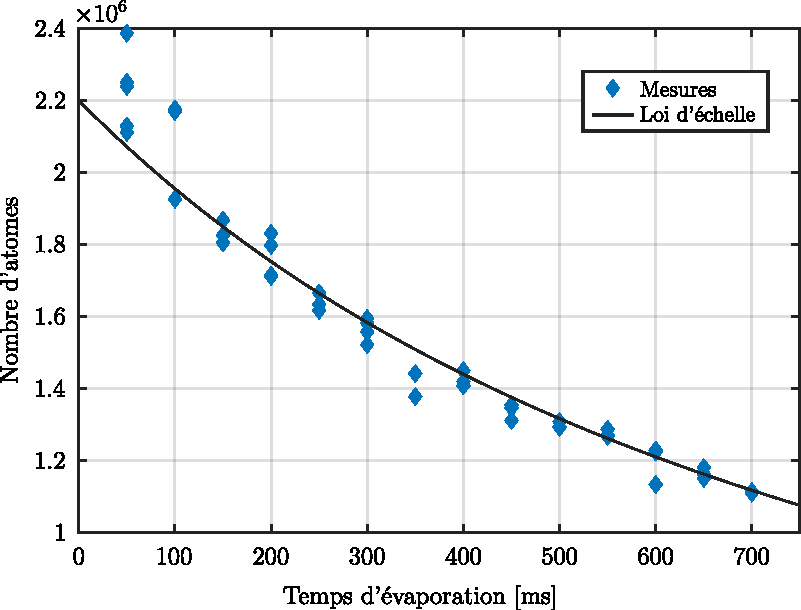
\includegraphics[width=0.7\textwidth]{Fig/modif_exp/Nombre_atomes_evap.pdf}
\caption{\textbf{Évolution du nombre d'atomes au cours de l'évaporation.} Les points bleus correspondent aux mesures expérimentales du nombre d'atomes, chaque point étant issu d'un unique cycle expérimental. La ligne continue noire correspond à la prédiction de la loi d'échelle \ref{eq:scaling_atomes_3corps} sans paramètre ajustable, avec les grandeurs $\eta=10$ et $R=0.1$ déterminées indépendamment. Il apparaît alors un très bon accord entre les données et le modèle.}
\label{fig:nombre_atomes_evap}
\end{figure}




\paragraph*{Évolution de la densité dans l'espace des phases}
Enfin, rappelons que l'optimisation de l'évaporation est réalisée en maximisant le gain de densité dans l'espace des phases par atome perdu, encodé par le paramètre $\gamma$. 

L'évolution de la densité dans l'espace des phases en fonction du nombre d'atomes est représentée figure \ref{fig:efficacite_evaporation_optique} en échelle logarithmique pour dans le cas de notre nouvelle consigne (en bleu) ainsi que pour notre ancienne consigne (en bordeaux). La comparaison est immédiate: la nouvelle consigne permet d'atteindre le seuil de condensation $\mathcal{D}\approx 1$ pour une perte d'atomes bien moindre que l'ancienne.

Plus quantitativement, l'efficacité mesurée pour la nouvelle consigne est de $\gamma\approx 4.5$ tandis que l'ancienne présente une efficacité d'environ 2.3\footnote{Cette mesure a été réalisée après le changement du laser source du piège optique. Avant changement, l'efficacité était plutôt estimée à 2.8 \citep{jendrzejewski2012quantum}.}, témoignant de la nette amélioration de notre évaporation. Notons que la loi d'échelle \ref{eq:efficacite_evap_3corps} en présence de pertes à trois corps prédit une valeur $\gamma\approx 6.5$, bien supérieure à notre valeur mesurée. Une étude approfondie de l'origine de cette différence n'a pas été menée compte-tenu de l'obtention récente de ces résultats et de l'excellente efficacité obtenue. En effet, la valeur de $\gamma\approx 3$ représente déjà une très bonne efficacité pour la plupart des expériences d'atomes ultra-froids \citep{barrett2001all}\citep{hung2008accelerating}.

Finalement, la consigne retenue à l'issue de l'optimisation de l'évaporation permet d'obtenir un condensat de Bose-Einstein d'environ \SI{1.2e6}{} atomes avec une température d'environ \SI{500}{\nano\kelvin} en \SI{700}{\milli\second}. Après \SI{3.5}{\second} d'évaporation, notre nuage contient environ \SI{2e5}{} atomes à une température de \SI{10}{\nano\kelvin} sans utiliser la technique d'ouverture adiabatique pour refroidir davantage. À l'heure de l'écriture de ces lignes, l'implémentation de cette technique avec la nouvelle consigne n'a pas encore été réalisée.


\begin{figure}
\centering
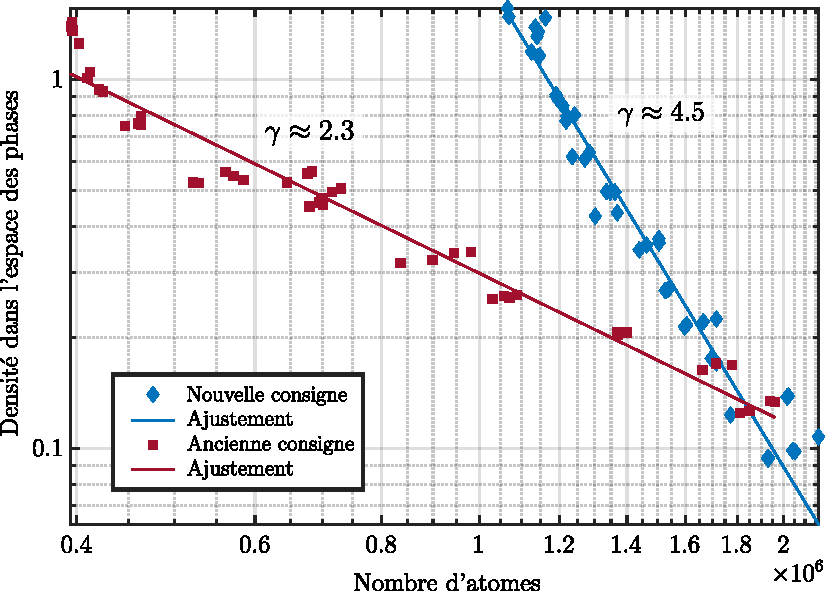
\includegraphics[width=0.8\textwidth]{Fig/Modif_exp/efficacité_évaporation_optique.pdf}
\caption{\textbf{Efficacité de l'évaporation optique.} En traçant la densité dans l'espace des phases du nuage en fonction du nombre d'atomes, on peut évaluer l'efficacité du refroidissement évaporatif. La nouvelle consigne d'évaporation permet d'obtenir les points bleus pour différents temps d'évaporation (jusqu'à \SI{700}{\milli\second}), tandis que l'ancienne consigne est représentée en bordeaux\protect\footnotemark\ (jusqu'à \SI{1.2}{\second}). Les lignes continues sont des ajustements des données expérimentales par des lois de puissance \ref{eq:efficacite_evaporation}, qui permettent ainsi d'extraire le paramètre $\gamma$ quantifiant l'efficacité de l'évaporation.}
\label{fig:efficacite_evaporation_optique}
\end{figure}
\footnotetext{Les données relatives à l'ancienne consigne ont été prises dans exactement les mêmes conditions expérimentales que celles relatives à la nouvelle: seule la consigne d'évaporation a été changée et ces données ont été obtenues les unes à la suite des autres.}


\chapterimage{Fig/Speckle/header2_wip.pdf}

\chapter{Propriétés d'un désordre de type \speckle}
\label{ch:Speckle}
%\begin{tikzpicture}[remember picture, overlay]
%\node[anchor=north east,inner sep=0pt] at (current page.north east) {\includegraphics[scale=1]{Fig/Speckle/g825.png}};
%\end{tikzpicture}

Le chapitre \ref{ch:BEC_manip} nous a renseigné quant aux propriétés de notre onde de matière ainsi que sa production. En particulier, on a vu qu'il était possible d'appliquer des potentiels externes conservatifs aux atomes par le biais du potentiel dipolaire. Ce potentiel étant proportionnel à l'intensité lumineuse $I$, on peut alors appliquer un désordre à nos atomes, pourvu que l'on soit capable de créer un désordre optique. En effet, une originalité de notre expérience est "d'inverser" les rôles habituels de la matière et de la lumière.

Ainsi, dans ce chapitre, nous allons nous attacher à décrire le second élément clé de la localisation d'Anderson: le désordre. Nous montrerons que la génération d'un tel désordre est aisée: la diffraction d'un faisceau laser au travers d'une lame de verre rugueuse produit un motif d'intensité lumineuse aléatoire et à fort contraste, appelé champs de tavelures optiques, ou encore \emph{Speckle} (anglicisme communément admis). Citons deux énormes avantages d'un tel désordre: on en connaît toutes les propriétés, régies par la diffraction, et on contrôle ce désordre. 

La première partie se concentrera sur la génération d'un champ de \speckle , en particulier sur le diffuseur qui donne au \speckle\ toutes ses propriétés. Dans un second temps, nous décrirons les propriétés spatiales d'un \speckle , en particulier la taille des grains de lumière dans les directions transverses et longitudinale. Dans une troisième partie nous parlerons du potentiel ressenti par les atomes ainsi que des possibilités offertes par la structure multi-niveaux du \isotope[87]{Rb} et l'excellent contrôle du désordre dont nous disposons, puis dans une ultime partie nous étudierons une approche à deux longueurs d'onde pour dépasser les limitations d'un \speckle\ monochromatique pour l'étude de la transition d'Anderson à énergie résolue. 

\section{Génération d'un champ de speckle}
%\section{Propriétés statistiques d'un champ de speckle}
C'est avec le développement des premiers lasers qu'a été observée la structure granulaire de la lumière réfléchie par certaines surfaces rugueuses. Rapidement, il a été compris que ce motif provenait de la diffraction aléatoire et cohérente par une surface rugueuse. 
Cette surface rugueuse peut-être considérée comme un ensemble d'émetteurs cohérents de déphasages aléatoires, et le profil d'intensité obtenu est le résultat de l'interférence multiple de l'ensemble de la surface. Un profil typique est montré figure \ref{fig:speckle_pattern}. Celui-ci comporte un ensemble de grains lumineux séparés par des zones d'obscurité.
Souvent considéré néfaste dans le domaine de l'imagerie, le \speckle\ est pour nous une source pratique de désordre optique. 

\begin{figure}
\centering
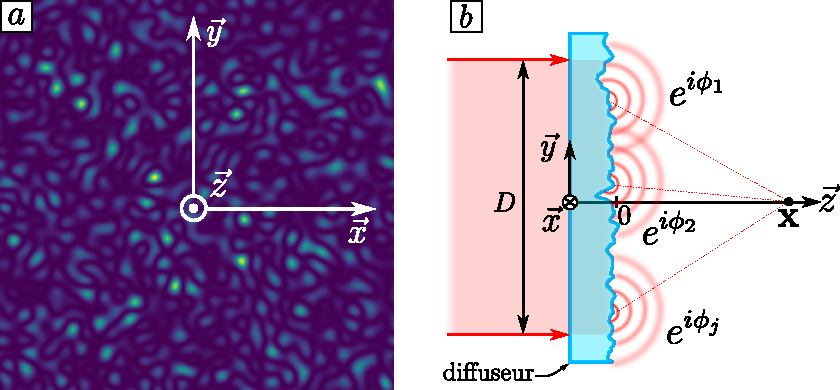
\includegraphics[width=0.9\textwidth]{Fig/Speckle/speckle_pattern.pdf}
\caption{\textbf{a: Génération d'une figure de speckle.} La diffraction d'une onde cohérente par une surface rugueuse appelée diffuseur résulte en l'interférence multiple d'une grand nombre d'ondes à déphasage aléatoire. La phase de chacune de ces ondes est déterminée par l'épaisseur de verre traversée en chaque point. \textbf{b: Motif de \speckle .} Un tel motif est composé de grains lumineux entourés de zones d'ombre, où l'intensité est quasiment nulle. }
\label{fig:speckle_pattern}
\end{figure}



\subsection{Statistiques de l'intensité d'un \speckle}
\label{sc:distribution_speckle}
Le phénomène de \speckle\ apparaît lorsque l'amplitude $E(\mathbf{x})$ au point d'observation $\mathbf{x}$ résulte de la somme d'un grand nombre N d'ondes indépendantes d'amplitude $E_0$ et de phases aléatoires $\phi_j$ comme illustré figure \ref{fig:speckle_pattern}.a. Cette amplitude peut alors s'écrire
\begin{equation}
E(\mathbf{x})=\sum_{j}^{N} E_0 e^{i \phi_j} \text{ .}
\end{equation}
En supposant qu'un grand nombre de grains du diffuseur participent à l'interférence au point d'observation ($\rdiff \ll D$ avec $\rdiff$ la taille typique d'un grain du diffuseur et $D$ la taille de l'éclairement incident), on peut appliquer le théorème central limite à l'amplitude rayonnée. En supposant de plus que les phases aléatoires $\phi_j$ sont réparties de manière homogène sur l'intervalle $\left[ 0,2\pi \right]$, les distributions de probabilités des parties réelle et imaginaire de l'amplitude sont données par la loi normale
\begin{equation}
\mathcal{P}(E_{\mathcal{R,I}})=\frac{1}{\sigma_E\sqrt{2\pi}} \exp{\left( -\frac{E_{\mathcal{R,I}}^2}{2 \sigma_E^2}\right) } \text{ ,}
\end{equation}
avec $E_{\mathcal{R}}$ et $E_{\mathcal{I}}$ les parties réelle et imaginaire du champ complexe $E=E_{\mathcal{R}} +i E_{\mathcal{I}}$ respectivement. Étant donné que les atomes ne sont sensibles qu'à l'intensité lumineuse $I=\left| E \right| ^2$, on montre alors que la distribution de probabilité de l'intensité lumineuse suit une loi exponentielle \citep{goodman2007speckle}
\begin{equation}
\mathcal{P}(I)=\frac{1}{\overline{I}}\exp{\left( -I/\overline{I} \right) } \text{ .}
\label{eq:proba_speckle}
\end{equation}
De manière générale, on appellera \emph{\speckle\ pleinement développé} tout \speckle\ vérifiant cette loi de probabilité. Deux conséquences importantes de cette loi sont à noter:
\begin{itemize}
\item[\textendash] L'écart-type $\sigma_I$ de la loi \ref{eq:proba_speckle} est égal à sa valeur moyenne $\overline{I}$, et donc le contraste $\sigma_I /\overline{I}$ d'une figure de \speckle\ pleinement développé est de 1. Une telle figure comportera alors des zones de forte intensité tout comme des zones d'intensité quasi-nulle. 
\item[\textendash] La probabilité d'obtenir une forte intensité lumineuse est exponentiellement petite, tandis que les zones de faible intensité sont beaucoup plus probables. Ainsi, une figure typique de \speckle\ (représentée figure \ref{fig:speckle_pattern}.b) est composée de maxima d'intensité lumineuse (\emph{grains de \speckle}) entourés de larges zones d'ombre.
\end{itemize}





\subsection{Propriétés du diffuseur}
\label{sc:prop_diffuseur}
L'analyse précédente décrivant la statistique de l'intensité lumineuse d'un \speckle\ pleinement développé repose sur deux hypothèses: 
\begin{itemize}
\item[\textendash] Il faut qu'un grand nombre d'émetteurs participe à l'interférence au point d'observation. Notamment, cela signifie que le diffuseur comporte un nombre suffisamment grand de \emph{grains} ($\rdiff \ll D$)  et que ceux-ci rayonnent au point d'observation. Ce dernier point sera illustré section \ref{sc:speckle_correlation}.
\item[\textendash] Pour que la distribution de probabilité de l'amplitude soit centrée en 0, propriété essentielle pour un \speckle\ pleinement développé, il faut que la distribution de phases soit suffisamment large de telle sorte que celle-ci puisse être considérée homogène sur l'intervalle $\left[ 0,2\pi \right]$. Cette condition de diffuseur fort se traduit en terme d'écart-type de la distribution de phases $\sigma_\phi \gg 2\pi$. 
\end{itemize}
Les deux grandeurs apparaissant dans ces hypothèses, $\rdiff$ et $\sigma_\phi$, sont fixées par les propriétés du diffuseur, que nous nous attacherons à décrire dans cette partie.

Dans le cadre de notre expérience, la génération du \speckle\ se fait par transmission d'une onde laser au travers d'une lame de verre dépolie, d'épaisseur locale $e(\mathbf{x}_0)$ aléatoire et répartie selon une distribution gaussienne de largeur $\sigmae$ et de valeur moyenne $\overline{e}$, où $\overline{\:\cdots\:}$ représente la moyenne sur les différentes réalisations de l'épaisseur aléatoire. On supposera que cette lame a été dépolie de manière homogène, ainsi, la statistique de l'épaisseur ne dépend pas de la position considérée sur la surface du diffuseur. On assimilera donc la distribution de l'épaisseur à un processus stationnaire. 

La phase localement accumulée par le faisceau laser incident lors de la traversée du diffuseur est proportionnelle à l'épaisseur traversée et donnée par
\begin{equation}
\phi(\mathbf{x}_0)=2\pi (n-1) \frac{e(\mathbf{x}_0)}{\lambda} \text{ ,}
\end{equation}
avec $n$ l'indice du verre et $\lambda\approx \SI{780}{\nano\metre}$ la longueur d'onde de l'onde laser. L'influence de cette phase sur l'amplitude du champ laser se traduit via la transmission locale du diffuseur
\begin{equation}
\tdiff(\mathbf{x}_0)=e^{i\phi(\mathbf{x}_0)}
\end{equation}
dont la valeur moyenne $\overline{\tdiff}$ caractérise le pouvoir diffusant. Pour une lame peu rugueuse, le faisceau est en moyenne peu affecté lors de sa traversée et l'on a $\overline{\tdiff}\approx 1$, tandis que dans le cas d'un diffuseur fort $\overline{\tdiff} \approx 0$. En fixant la phase moyenne $\overline{\phi}=0$, on montre annexe \ref{ch:anex_speckle} que \citep{denechaud2018vers}
\begin{equation}
\overline{\tdiff}=e^{-\frac{\sigma_{\phi}^2}{2}} \quad \text{avec} \quad \sigma_\phi=2\pi (n-1) \frac{\sigmae}{\lambda} \text{ .}
\label{eq:sigma_phi}
\end{equation}
Dans le cas d'un diffuseur de grande rugosité, dont l'épaisseur typique des grains $\sigmae$ est de l'ordre de plusieurs $\lambda$, on a $\sigma_\phi \gg 2\pi$ et cela permet donc de considérer que la distribution de phases est constante sur l'intervalle $\left[0,2\pi \right]$, essentiel pour un \speckle\ pleinement développé.

\begin{figure}
\centering
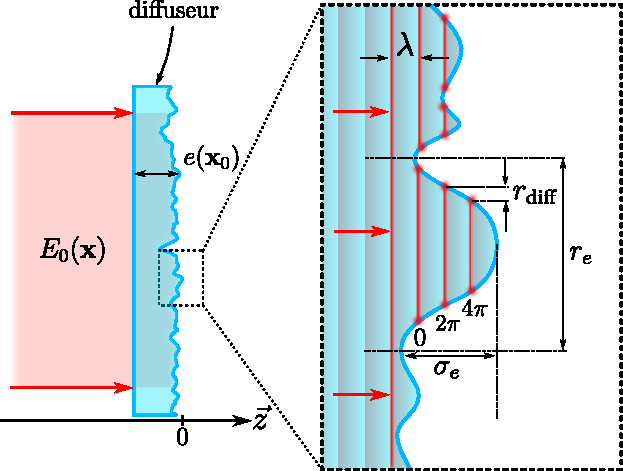
\includegraphics[scale=1]{Fig/Speckle/diffus_prop.pdf}
\caption{\textbf{Caractéristiques du diffuseur.} L'épaisseur aléatoire est caractérisée par une hauteur typique $\sigmae$ et une granularité de taille $r_e$. Pour $\sigmae \gg \lambda$, on a plusieurs oscillations de l'onde incidente dans le même grain, et donc $\tdiff$ qui est une fonction $2\pi-$périodique, voit sa corrélation réduite.}
\label{fig:diffus_prop}
\end{figure}

Les grains du diffuseur sont de plus caractérisés par une certaine extension spatiale typique $r_e$ correspondant à une largeur de corrélation de l'épaisseur. Celle-ci induit donc une corrélation spatiale de la transmission, décrite à l'aide la fonction de corrélation
\begin{equation}
\Cdiff(\mathbf{x}_0,\mathbf{x}'_0)=\overline{\tdiff(\mathbf{x}_0)\tdiff^*(\mathbf{x}'_0)}=\overline{e^{i(\phi(\mathbf{x}_0)-\phi(\mathbf{x}'_0))}} { .}
\label{eq:correlation_diffuseur}
\end{equation}

Puisque l'épaisseur et la phase sont proportionnelles, ces deux grandeurs sont corrélées sur la même taille $r_e$ correspondant à la granularité de la surface du verre. En revanche, dans le cas où $\sigmae \gg \lambda$ (ce qui est le cas sur notre expérience), l'onde oscille plusieurs fois dans le même grain du diffuseur. La transmission étant une fonction $2\pi-$périodique de la phase, celle-ci perd alors sa corrélation sur une taille $\rdiff \ll r_e$, voir figure \ref{fig:diffus_prop}. On montre alors annexe \ref{ch:anex_speckle} que la corrélation de la transmission à courte portée\footnote{La corrélation de la transmission tend suffisamment vite vers 0 pour que l'on puisse considérer que $\left|\mathbf{x}_0-\mathbf{x}'_0 \right| \ll r_e$ dans le cas où $\sigma_\phi \gg 2\pi$.} est de forme gaussienne:
\begin{equation}
\Cdiff(\mathbf{x}_0,\mathbf{x}'_0)\approx \exp{\left( -\frac{\left| \mathbf{x}_0 - \mathbf{x}'_0 \right| ^2}{2 \rdiff^2}\right) } \quad \text{avec} \quad \rdiff=r_e/\sigma_\phi \text{ .}
\label{eq:formule_Cdiff}
\end{equation}
$\rdiff$ joue alors le rôle de la taille effective d'un émetteur indépendant tel que considéré dans la section \ref{sc:distribution_speckle}. La condition d'un grand nombre d'émetteurs s'écrit alors $\rdiff \ll D$.

Enfin, il est possible de définir l'angle de diffusion $\theta_{\mathrm{diff}}=\lambda/\pi \rdiff=2(n-1) \sigmae/r_e$, qui est indépendant de la longueur d'onde de l'onde laser incidente. $\theta_{\mathrm{diff}}$ est donc une constante du diffuseur, fixée par les paramètres géométriques de celui-ci.










\subsection{Implémentation expérimentale}
\label{sc:montage_diffuseur}
Les expériences menées sur notre dispositif jusqu'en 2014 utilisaient un \speckle\ réalisé à la longueur d'onde de \SI{532}{\nano\metre}. Ce grand désaccord vers le bleu par rapport à la transition $\mathrm{D}_2$ du \isotope[87]{Rb} permet ainsi de s'affranchir de l'émission spontanée, même pour les très longs temps de propagation nécessaires à l'étude de la localisation d'Anderson. Depuis 2015 en revanche, l'équipe utilise un \speckle\ accordable autour de \SI{780}{\nano\metre} offrant ainsi la possibilité de réaliser un désordre attractif ou répulsif. Nous verrons section \ref{sc:potentiel_speckle} que cette accordabilité autour de la transition $\mathrm{D}_2$ offre un grand nombre de possibilités expérimentales, telles que la génération d'un désordre dépendant du spin.

\paragraph*{Mise en forme du faisceau \speckle}

\begin{figure}
\centering
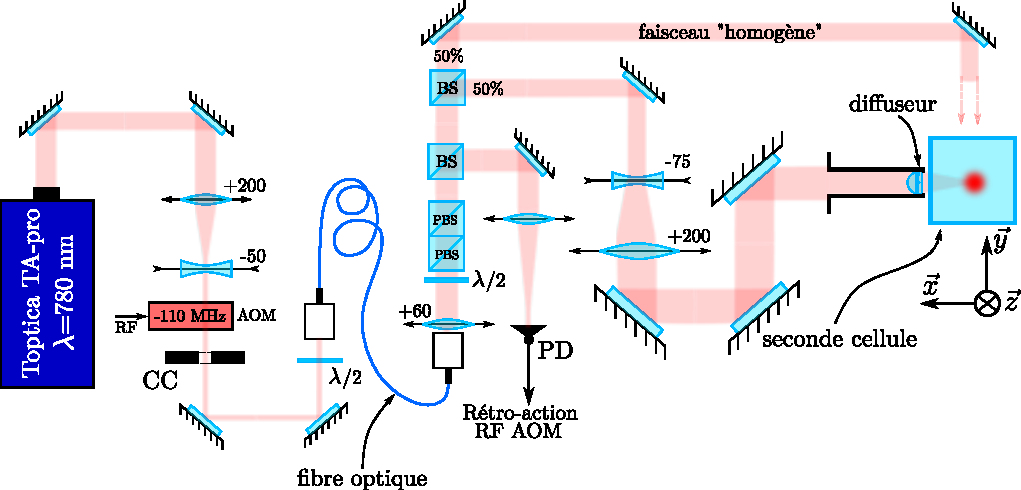
\includegraphics[width=\textwidth]{Fig/Speckle/montage_speckle_taus.pdf}
\caption{\textbf{Montage de génération du désordre optique.} Ce montage se décompose en deux parties, la première étant dédiée à la mise en forme du faisceau (cadre de gauche). Celui-ci est émis d'un laser Toptica TA-Pro, dont le mode et la polarisation sont filtrés, et la puissance est stabilisée. Dans un second temps, ce faisceau est focalisé sur les atomes et passe au travers du diffuseur générant le \speckle\ (cadre de droite).}
\label{fig:montage_speckle_taus}
\end{figure}

Par vœux de concision, seules les grandes lignes du montage de génération du \speckle\ à \SI{780}{\nano\metre} seront données ici, de nombreux détails à propos de ce montage pouvant être retrouvés dans les thèses de Jérémie Richard, Vincent Denechaud et Musawwadah Mukhtar \citep{denechaud2018vers, mukhtar2019state, richard2015propagation}. De plus, les détails des éléments du montage dépendent fortement de la mesure souhaitée comme nous le verrons dans la suite de chapitre, néanmoins la philosophie en reste inchangée.

Ce montage se décompose en deux parties, la première permettant de mettre en forme les propriétés du faisceau laser, et la seconde génère le désordre sur les atomes.

Le faisceau source du \speckle\ est émis par un laser industriel \emph{Toptica TA-Pro} \SI{2}{\watt} accordable autour de \SI{780}{\nano\metre}. Étant donné la proximité de la transition atomique, ce laser peut être asservi par battements sur le laser repompeur \emph{L2}\footnote{Le choix d'asservir ou non ce laser dépend du désaccord utilisé. Ainsi, nous verrons que le laser \speckle\ n'était pas asservi en fréquence pour la mesure du temps de diffusion élastique ($\left|\Delta\right|/2\pi\sim\SI{1}{\tera\hertz}$), tandis que ce fut le cas lors de la mesure des fonctions spectrales ($\left|\Delta\right|/2\pi\sim\SI{70}{\mega\hertz}$).}, ce qui permet alors d'en fixer la fréquence avec une précision de \SI{1}{\mega\hertz}. Le mode spatial et la polarisation du faisceau sont filtrés à l'aide d'une fibre optique à maintien de polarisation et de cubes séparateurs de polarisation. 

Une partie de la puissance du faisceau est ensuite prélevée et mesurée à l'aide d'une photodiode, et la rétroaction sur le faisceau à l'aide d'un modulateur acousto-optique (AOM pour l'anglais \emph{Acousto-Optic Modulator}) permet alors d'en stabiliser la puissance. La photodiode étant placée après la fibre optique et les cubes séparateurs de polarisation, la boucle d'asservissement de puissance permet de plus de s'affranchir des fluctuations de puissance dues à la polarisation et aux fluctuations du couplage. 

Enfin, le faisceau est séparé en deux parties par une séparatrice $50/50$, chacune de ces parties pouvant être envoyée sur les atomes. La partie réfléchie est ensuite agrandie à l'aide d'un télescope avant d'être focalisée sur les atomes et diffraction par le diffuseur, dont la géométrie sera présentée dans le paragraphe suivant. À ce stade, on dispose d'un faisceau de waist \SI{14.6}{\milli\metre} (rayon à $1/e^2$), de polarisation $\pi$ et dont la puissance est stabilisée et contrôlable.

Historiquement, la partie transmise était utilisée afin de réaliser une superposition cohérente de deux faisceaux \speckle , permettant d'obtenir un désordre isotrope\footnote{Comme nous le verrons section \ref{sc:correlation_longitudinale}, les grains d'un \speckle\ unique sont étendus suivant la direction longitudinale. L'interférence entre deux \speckles\ croisés permet de fortement réduite cette anisotropie \citep{piraud2012localisation}.} \citep{jendrzejewski2012quantum}. Aujourd'hui, ce faisceau est utilisé sans diffuseur et permet de réaliser un potentiel homogène servant à calibrer l'amplitude du potentiel.




%La spécificité de ce montage réside dans sa capacité à stabiliser par asservissement une très faible puissance optique, typiquement de quelques \SI{}{\micro\watt} compte-tenu de la proximité de la transition. Pour cela, 90\% de la puissance optique sont déviés vers une photodiode, dont la mesure permet de rétroagir sur la puissance du faisceau à l'aide d'un modulateur acousto-optique. Cette mesure à haute puissance permet de plus d'être particulièrement sensible aux fluctuations de puissance. 





\paragraph*{Génération du \speckle}

\begin{figure}
\centering
\includegraphics[width=0.9\textwidth]{Fig/Speckle/montage_diffuseur.pdf}
\caption{\textbf{Géométrie du montage de génération du \speckle .} Un faisceau gaussien incident de waist \SI{14.6}{\milli\metre} est tronqué dans un diaphragme de diamètre \SI{22.9}{\milli\metre} qui supporte le diffuseur. Ce faisceau est ensuite focalisé par une lentille asphérique épaisse de focale \SI{16}{\milli\metre} et traverse le diffuseur d'épaisseur \SI{0.5}{\milli\metre}. Le plan de focalisation est déplacé d'environ \SI{1}{\milli\metre} à cause de la paroi de la cellule à vide, d'épaisseur \SI{3}{\milli\metre}. Le plan repéré en rouge, correspondant à la surface moyenne du diffuseur, servira de plan de référence dans le cadre d'une géométrie effective illustrée figure \ref{fig:geometrie_effective_speckle}.}
\label{fig:montage_diffuseur}
\end{figure}

La génération du \speckle\ se fait selon le montage représenté figure \ref{fig:montage_diffuseur}. Un faisceau gaussien collimaté de waist \SI{14.6}{\milli\metre} et de longueur d'onde $\lambda=\SI{780}{\nano\metre}$, dont la mise en forme a été présentée dans le paragraphe précédent, est tronqué par un diaphragme de diamètre \SI{22.9}{\milli\metre}. Ce faisceau passe ensuite au travers d'une lentille asphérique épaisse (\textit{Thorlabs ACL2520-B}) de focale \SI{16.0}{\milli\metre} (et de frontale \SI{15.7}{\milli\metre}) montée dans ce même diaphragme. Le rôle de celle-ci est de focaliser la lumière sur les atomes\footnote{Nous verrons dans la section suivante que cela permet d'obtenir des grains de \speckle\ les plus petits possibles. En effet, on attend la manifestation d'effets quantiques sur la propagation d'une onde de matière dans un \speckle\ pour des longueurs d'onde de de Broglie plus grandes que la taille des grains de \speckle .}. Accolé à cette lentille se trouve un diffuseur \textit{Newport FSD10-3} possédant une épaisseur de \SI{0.5}{\milli\metre}\footnote{Cette épaisseur était initialement de \SI{3}{\milli\metre} avant d'être réduite à \SI{0.5}{\milli\metre} par l'atelier d'optique de l'IOGS.} et un angle de diffusion $\theta_{\mathrm{diff}}\approx\SI{5}{\degree}$. 

Enfin, ce faisceau convergent traverse la paroi de la cellule en verre sous ultra-vide d'épaisseur $e=\SI{3.0}{\milli\metre}$ et située à \SI{0.5}{\milli\metre} de la monture du diffuseur. Le matériau de cette cellule est du Vycor, d'indice optique $n=1.46$. L'épaisseur de cette cellule, considérée comme une lame à faces parallèles, induit un décalage des rayons lumineux par réfraction, décalage représenté figure \ref{fig:montage_diffuseur} montrant la trajectoire des rayons lumineux en absence de la paroi par des traits pointillés. La présence de la paroi entraîne donc un déplacement du plan de focalisation donné par $\Delta d=e(1-1/n)\approx \SI{1}{\milli\metre}$. La distance focale en présence de la paroi de la cellule est alors de \SI{17.0}{\milli\metre}.


En choisissant pour origine de l'axe $\vec{z}$\footnote{L'axe $\vec{z}$ utilisé dans ce chapitre correspond à la direction de propagation du faisceau \speckle . Dans le repère de l'expérience, il s'agit en réalité de l'axe $\vec{x}$, perpendiculaire au plan formé par les faisceaux du piège optique.} la surface du diffuseur, la position du plan de focalisation se trouve à $f=\SI{16.2}{\milli\metre}$. Dans ce repère, la position des atomes dans le piège optique est estimée quant à elle a $d=16\pm\SI{0.5}{\milli\metre}$, dont la valeur est proche de celle de la position du plan de focalisation. Néanmoins, l'incertitude liée à la position des atomes est cruciale, celle-ci pouvant conduire à un écart de \SI{0.7}{\milli\metre} du plan de focalisation. Il est ainsi primordial de connaître les propriétés du \speckle\ autour du plan de focalisation. 


\paragraph*{Géométrie effective du montage du diffuseur}
La lentille asphérique utilisée pour la focalisation du faisceau sur les atomes étant épaisse\footnote{L'épaisseur au centre est de \SI{12}{\milli\metre} pour une frontale de \SI{15.7}{\milli\metre}.}, le faisceau est donc fortement affecté par sa traversée. L'éclairement dans le plan du diffuseur correspond donc à l'éclairement incident gaussien de waist \SI{14.6}{\milli\metre} (rayon à $1/e^2$) tronqué par une pupille de diamètre \SI{22.9}{\milli\metre} et ayant déjà subi un effet de focalisation. Il a été déterminé par photographie que le profil de l'éclairement dans le plan du diffuseur est aussi de forme gaussienne tronquée, avec un waist $w_0=9\pm\SI{1}{\milli\metre}$ et une pupille de diamètre $D=20.3\pm\SI{0.1}{\milli\metre}$.

Il est alors possible de décrire le montage du diffuseur et le champ incident à l'aide d'une géométrie effective simplifiée illustrée figure \ref{fig:geometrie_effective_speckle}. On considèrera ainsi que le profil d'intensité au niveau du diffuseur est donné par une forme gaussienne de largeur $w=9\pm\SI{1}{\milli\metre}$ tronquée par une diaphragme de diamètre $D=20.3\pm\SI{0.1}{\milli\metre}$ et convergeant à la distance $f=\SI{15.2}{\milli\metre}$\footnote{Si la présence de la paroi de la cellule entraîne un déplacement du plan focalisation, celle-ci ne modifie pas l'ouverture numérique du système, c'est-à-dire l'angle des rayons avec l'axe optique. Comme nous le verrons dans la suite, il s'agit de la quantité qui décrit, avec la longueur d'onde, les propriétés spatiales d'un champ de \speckle .}. Ceci entraîne une ouverture numérique maximale $\ON=\sin{(\theta_{\mathrm{max}})}=0.55\pm0.02$. Dans le cadre de cette géométrie effective, la position des atomes est estimée à $d=15\pm\SI{0.5}{\milli\metre}$.

\begin{figure}
\centering
\includegraphics[scale=0.9]{Fig/Speckle/geometrie_effective_speckle.pdf}
\caption{\textbf{Géométrie effective du montage du diffuseur.} L'épaisseur de la lentille n'étant pas négligeable, l'éclairement au niveau du diffuseur a déjà subi un effet de focalisation comparé à celui au niveau de la lentille. Cela se traduit par un front d'onde au niveau du diffuseur qui est convergeant, avec un profil gaussien de largeur $w\approx\SI{9}{\milli\metre}$ tronqué à un diamètre $D\approx\SI{20.3}{\milli\metre}$.}
\label{fig:geometrie_effective_speckle}
\end{figure}


\paragraph*{Amplitude rayonnée}
L'utilisation de ce modèle à géométrie effective permet de décrire simplement les propriétés du champ de \speckle . En particulier, l'amplitude rayonnée $E(\xd)$ est simplement donnée par le principe de Huygens-Fresnel\footnote{Nous utilisons ici l'approximation paraxiale (voir annexe \ref{ch:anex_speckle}), dont la pertinence sera discutée à postériori.}:
\begin{equation}
E(\xd) \propto \int{\mathrm{d}\xzero \: \Ediff (\xzero) \exp{\left( ik\frac{\xzero^2}{2\deff} \right) } \: \exp{\left( -ik \frac{\xd \cdot \xzero}{d} \right) } } \text{ ,}
\label{eq:amplitude_rayonnee}
\end{equation}
où l'ensemble des points $\lbrace\xd\rbrace$ correspond au plan $\lbrace x,y,z=d \rbrace$ situé à une distance $d$ de la surface du diffuseur. L'ensemble des points $\lbrace\xzero\rbrace$ décrit le plan du diffuseur $\lbrace x,y,z=0 \rbrace$, $k=2\pi/\lambda$ est le nombre d'onde et $\deff$ correspond à une distance effective donnée par $1/\deff=1/d-1/f$.

$\Ediff (\xzero)$ correspond à l'amplitude dans le plan de référence du diffuseur, qu'il est possible de décomposer sous la forme 
\begin{equation}
\Ediff(\xzero)=\Ezero(\xzero) \tdiff(\xzero) \quad \text{avec} \quad \Ezero(\xzero) = E_\mathrm{inc} (\xzero) m(\xzero) \text{ ,}
\end{equation}
où $\tdiff(\xzero)$ est la transmission du diffuseur, $E_{\mathrm{inc}}(\xzero)$ est le champ incident\footnote{Il s'agit du faisceau gaussien de waist \SI{9}{\milli\metre} dans notre géométrie effective.}, et $m(\xzero)=\Theta(\left| \xzero \right| - D/2)$ avec $\Theta$ la fonction de Heaviside est un masque représentant le diaphragme de diamètre $D$. $\Ezero(\xzero)$ correspond alors au champ au niveau du diffuseur, de forme gaussienne tronquée et convergente.


\section{Propriétés spatiales d'un champ de \speckle}
\label{sc:speckle_correlation}

Le \speckle\ résultant de la propagation d'un faisceau transmis par le diffuseur, il est donc régit par les lois de la diffraction. Il est donc possible de déduire les propriétés spatiales du \speckle\ de celles du diffuseur ainsi que de celles de l'éclairement incident. Notamment, les variations spatiales du champ de \speckle\ sont décrites quantitativement par sa fonction de corrélation, dont l'étude permet de déterminer toutes les tailles caractéristiques d'intérêt pour notre expérience. Parmi celles-ci, nous nous concentrerons sur l'extension du champ de \speckle\ ainsi que sur les tailles moyennes des grains de lumière. 

Dans cette section, nous allons nous attacher à décrire ces échelles de longueur caractéristiques autour du plan de focalisation à l'aide de la fonction de corrélation du champ de \speckle\ et de son intensité moyenne, dont le détail des calculs est donné en annexe \ref{ch:anex_speckle}. 

De plus, lors de la conception de ce système, l'extension du champ de \speckle\ ainsi que les tailles des grains de \speckle\ ont été mesurées expérimentalement sur un montage reproduisant exactement les conditions réelles en présence de la cellule à vide, celle-ci empêchant de faire des mesures in-situ. La description de ces mesures et de leur traitement sont référencées dans la thèse de Jérémie Richard \citep{richard2015propagation}.




\subsection{Extension transverse du champ de speckle le long le l'axe optique}
%%%%%%%%%%%%%%%%%%%%%%%%%%%%%%%%%%%%%%%%
\begin{comment}
Afin de déterminer l'extension transverse du champ de \speckle , il est nécessaire de calculer le profil d'intensité moyenne $\overline{I}(\xd)$, où l'ensemble des points $\lbrace\xd\rbrace$ correspond au plan $\lbrace x,y,z=d \rbrace$ situé à une distance $d$ de la surface du diffuseur. Pour cela, explicitons le champ rayonné $E(\xd)$ à l'aide du principe de Huygens-Fresnel dans l'approximation paraxiale:
\begin{equation}
E(\xd) \propto \int{\mathrm{d}\xzero \: \Ediff (\xzero) \exp{\left( ik\frac{\xzero^2}{2\deff} \right) } \: \exp{\left( -ik \frac{\xd \cdot \xzero}{d} \right) } } \text{ ,}
\label{eq:amplitude_rayonnee}
\end{equation}
où $k=2\pi/\lambda$ est le nombre d'onde et $\deff$ correspond à une distance effective donnée par $1/\deff=1/d-1/f$. L'ensemble des points $\lbrace\xzero\rbrace$ décrit le plan du diffuseur $\lbrace x,y,z=0 \rbrace$, et $\Ediff (\xzero)$ correspond au champ dans ce plan, qu'il est possible de décomposer sous la forme 
\begin{equation}
\Ediff(\xzero)=\Ezero(\xzero) \tdiff(\xzero) \quad \text{avec} \quad \Ezero(\xzero) = E_\mathrm{inc} (\xzero) m(\xzero) \text{ ,}
\end{equation}
où $\tdiff(\xzero)$ est la transmission du diffuseur, $E_{\mathrm{inc}}(\xzero)$ est le champ incident\footnote{Il s'agit du faisceau gaussien de waist \SI{9}{\milli\metre} dans notre géométrie effective.}, et $m(\xzero)=\Theta(\left| \xzero \right| - D/2)$ avec $\Theta$ la fonction de Heaviside est un masque représentant le diaphragme de diamètre $D$. $\Ezero(\xzero)$ correspond alors au champ au niveau du diffuseur, et on supposera dans la suite que celui-ci varie lentement à l'échelle des variations de $\tdiff(\xzero)$, c'est-à-dire que $\Ezero(\xzero+\delta\xzero)\approx\Ezero(\xzero)$ avec $\delta\xzero$ de l'ordre de $\rdiff$.
\end{comment}
%%%%%%%%%%%%%%%%%%%%%%%%%%%%%%%%%%%%%%%%%%%%%%%%

Afin de déterminer l'extension transverse du champ de \speckle , il est nécessaire de calculer le profil d'intensité moyenne $\overline{I}(\xd)$ à partir de l'expression de l'amplitude rayonnée \ref{eq:amplitude_rayonnee}. En remarquant que le champ $\Ezero(\xzero)$ varie lentement à l'échelle des variations de $\tdiff(\xzero)$, on peut écrire que $\Ezero(\xzero+\delta\xzero)\approx\Ezero(\xzero)$ avec $\delta\xzero$ de l'ordre de $\rdiff$. 

On montre alors (voir annexe \ref{ch:anex_speckle}) que le profil d'intensité moyenne à la distance $d$ peut s'écrire \citep{gatti2008three}
\begin{align}
\nonumber\overline{I}(\xd)&=\overline{E(\xd) E^*(\xd)} \\
&\propto I_0 \left( \frac{\deff}{d} \xd \right) \ast \widetilde{\Cdiff}\left( \frac{\xd}{\lambda d} \right) \text{ ,}
\label{eq:evolution_extension_transverse_speckle}
\end{align}
où le symbole $\ast$ dénote le produit de convolution. L'évolution du profil d'intensité moyenne en fonction de la distance $d$ est alors dû à deux contributions dont l'interprétation physique est la suivante:
\begin{itemize}
\item[\textendash] Le premier terme correspond à l'effet de la lentille dans le cadre de l'optique géométrique, et focalise donc le profil d'intensité initiale $I_0(\xzero)=\left| \Ezero(\xzero) \right|^2$ dans le plan focal $\lbrace x,y,z=f\rbrace$. Cette focalisation se traduit au travers d'un changement d'échelle de l'intensité par le facteur $d/\deff=\left| d-f \right| /f$. Ainsi, la taille de ce faisceau focalisé décroît avec la distance jusqu'à s'annuler dans le plan focal, comme prédit par l'optique géométrique.
\item[\textendash] Le second terme est la transformée de Fourier de la fonction de corrélation du diffuseur $\Cdiff(\xzero)$. Ce terme traduit la diffraction de l'onde incidente par les grains du diffuseur de taille $\rdiff$. À partir de l'expression \ref{eq:formule_Cdiff} de $\Cdiff(\xzero)$, on trouve que ce terme correspond à une gaussienne dont la largeur est donnée par $\lambda d/ \pi \rdiff$, qui croît linéairement avec la distance $d$.
\end{itemize}
Ces dépendances sont illustrées figure \ref{fig:speckle_extension}, où le fond rose correspond au premier terme de focalisation, tandis le fond orange illustre le second terme de diffraction issu du centre du diffuseur. On identifie alors deux régimes pour lesquels un terme est prépondérant. 

\begin{figure}
\centering
\includegraphics[width=\textwidth]{Fig/Speckle/speckle_extension.pdf}
\caption{\textbf{Extension du champ de speckle.} L'extension du faisceau de speckle est due à deux effets distincts, la focalisation du faisceau incident et la diffraction du faisceau par le diffuseur suivant un angle $\theta_{\mathrm{diff}}$. La contribution de la focalisation à l'extension du faisceau est illustrée par des flèches rouges et un remplissage rose, tandis que celle de la diffraction correspond à un remplissage orange. La région aux alentours du plan focal est particulièrement intéressante car il s'agit de celle où l'ensemble des émetteurs contribuent à l'éclairement, chaque émetteur diffractant dans un cône d'angle $\theta_{\mathrm{diff}}$ illustré par des pointillés rouges. Dans le cas où l'angle de diffusion est petit devant l'ouverture numérique $\theta_{\mathrm{diff}} \ll \ON$, on peut estimer par trigonométrie l'étendue de cette région à $\delta f/2= \speckleext / \ON$ (encart).}
\label{fig:speckle_extension}
\end{figure}

Dans une première région, loin du plan focal de la lentille, la taille du faisceau est donnée par l'effet de focalisation de la lentille. Une seconde région, proche du plan focal de la lentille, est dominée par l'effet de diffraction des émetteurs du diffuseur, la taille de l'éclairement incident étant fortement réduite par focalisation. Ainsi, pour une zone très proche du plan focal de la lentille, on peut décrire le profil d'intensité lumineuse par 
\begin{equation}
\overline{I}\propto \mathrm{TF} \left[ \Cdiff \right] (\xf/\lambda f)
\end{equation}
où l'ensemble des points $\lbrace \xf \rbrace$ correspond au plan de Fourier\footnote{Dans le plan focal $\lbrace x,y,z=f\rbrace$, le champ rayonné est alors la transformée de Fourier du champ incident comme illustré par la formule \ref{eq:amplitude_rayonnee}. Il s'agit d'une propriété bien connue des lentilles de pouvoir ramener l'infini de la diffraction de Fraunhofer à distance finie.} $\lbrace x,y,z=f \rbrace$, et $\Cdiff$ est la fonction de corrélation du diffuseur, de forme de gaussienne avec une largeur $\rdiff$. Le profil d'intensité lumineuse dans le plan de Fourier est alors donné par 
\begin{equation}
\overline{I}(\xf)\propto \exp{(-\frac{2 \left| \xf \right|^2}{\speckleext})} \quad \text{avec} \quad \speckleext = \frac{\lambda f}{\pi \rdiff} \text{ .}
\label{eq:intensite_moyenne_speckle}
\end{equation}
$\speckleext$ correspond donc au waist du profil d'intensité moyenne, dont l'expression peut se réécrire à l'aide de l'angle du diffusion $\speckleext=\theta_{\mathrm{diff}} f = 1.5\pm\SI{0.1}{\milli\metre}$. Donc, dans le plan de Fourier, l'extension du champ de \speckle\ ne provient que de l'effet de la diffraction des émetteurs individuels dont les faisceaux se recouvrent tous, comme illustré figure \ref{fig:speckle_extension} par la zone orange.

Cette condition de recouvrement des faisceaux provenant de l'ensemble des émetteurs du diffuseur permet de considérer que dans cette région le \speckle\ est entièrement développé. Afin d'en déterminer l'étendue longitudinale, on s'intéresse aux positions de l'espace où l'ensemble des faisceaux provenant du diffuseur participent. Dans la limite $\theta_{\mathrm{diff}} \ll \ON$, on détermine par trigonométrie que cette zone s'étend de part et d'autre du plan de Fourier sur une distance $\delta f/2\approx \speckleext /\ON =2.5\pm\SI{0.1}{\milli\metre}$ (voir figure \ref{fig:speckle_extension}), délimitant ainsi les régions décrites précédemment. Par analogie avec un faisceau gaussien, on appellera $\delta f$ la \emph{distance de Rayleigh} du champ de \speckle , et sa valeur nous assure que les atomes se trouveront dans la zone où le \speckle\ est pleinement développé, celle-ci étant un ordre de grandeur plus grande que l'incertitude de positionnement des atomes.















\subsection{Longueur de corrélation transverse le long de l'axe optique}
\label{sc:correlation_transverse}
La seconde taille caractéristique du \speckle , la taille des grains de lumière, est une grandeur d'une importance capitale pour la physique du désordre. Si l'extension du faisceau de \speckle\ est une grandeur d'intérêt pratique (celle-ci donne une borne supérieure sur les tailles de nuages et détermine le potentiel maximal accessible en fonction de la puissance du faisceau laser), nous verrons chapitre \ref{ch:TauS_PRL} que la taille des grains de \speckle\ influe sur la dynamique de la propagation d'une onde en milieu désordonné.

Le potentiel ressenti par les atomes étant proportionnel à l'intensité lumineuse, on peut définir la taille des grains du potentiel à l'aide de la fonction de corrélation en intensité du \speckle . En utilisant le théorème de Wick pour les variables aléatoires gaussiennes, il est possible de relier la fonction de corrélation en intensité à la fonction de corrélation en amplitude du \speckle :
\begin{equation}
\overline{I(\xd) I(\xd')}=\overline{I(\xd)}\;\overline{I(\xd')} + \left| \overline{E(\xd)E^*(\xd')} \right|^2 \text{ ,}
\label{eq:theoreme_wick}
\end{equation}
où les positions $\xd$ et $\xd'$ correspondent à deux points dans le plan $\lbrace x,y,z=d\rbrace$ transverse à l'axe optique. 

Dans les conditions expérimentales usuelles, il est possible de négliger l'effet de l'extension spatiale finie du \speckle , celle-ci étant très grande à l'échelle des grains de \speckle . Dans ce régime, on peut alors considérer que le premier terme de l'équation \ref{eq:theoreme_wick} est constant et égal à $\overline{I}^2$. On définit alors la taille des grains du potentiel à l'aide la fonction de corrélation des fluctuations d'intensité:
\begin{equation}
\overline{\delta I(\xd) \delta I(\xd')} = \left| \overline{E(\xd)E^*(\xd')} \right|^2 \text{ ,}
\end{equation}
où $\delta I(\xd)=I(\xd)-\overline{I}(\xd)$ correspond aux fluctuations statistiques d'intensité. 

À l'échelle des grains de \speckle , on peut considérer que la fonction de corrélation en amplitude ne dépend uniquement que de la différence des positions considérées. On montre annexe \ref{ch:anex_speckle} que la fonction de corrélation transverse en amplitude le long de l'axe optique peut s'écrire \citep{gatti2008three}:
\begin{align}
\nonumber \CE(\xd,\xd') &= \overline{E(\xd) E^*(\xd')} \\
& \propto \widetilde{I_0}\left( \frac{\delta\xd}{\lambda d}\right) \ast \Cdiff\left( \frac{\deff}{d} \delta \xd \right) \text{ ,}
\label{eq:correlation_transverse_speckle}
\end{align}
où $\delta\xd=\xd'-\xd$. De même que pour l'extension spatiale du champ de \speckle , la fonction de corrélation transverse résulte de deux contributions, dont les interprétations physiques sont les suivantes:
\begin{itemize}
\item[\textendash] Le premier terme correspond à la transformée de Fourier de l'intensité lumineuse dans le plan du diffuseur. Il s'agit ici du motif de diffraction à l'infini en l'absence du diffuseur, dont la taille est proportionnelle à la distance. Ce facteur d'échelle s'interprète comme une diminution de l'ouverture numérique au fur et à mesure de l'éloignement avec le diffuseur, comme indiqué par la relation $\ON'(d)=D/2d$ en considérant les rayons les plus inclinés, avec $D$ la taille du diaphragme de l'éclairement au niveau du diffuseur. Ce terme conduit donc à largeur de l'ordre de $\sim\lambda / \pi \ON'(d)$, qui croît linéairement avec la distance $d$. 
\item[\textendash] Le second terme décrit quant à lui le fait que les grains du diffuseur ne diffractent que selon un angle $\theta_{\mathrm{diff}}$. De fait, ce terme décrit les régions de l'espace dans lesquelles l'ensemble du diffuseur ne participe pas à l'interférence au point $\xd$, comme illustré par la zone orange figure \ref{fig:correlation_speckle}. Ce terme joue ainsi le rôle d'ouverture numérique effective, dont l'expression $\ON_{\mathrm{eff}}(d)=\theta_{\mathrm{diff}} f/\left| d-f \right|$ peut être obtenue par trigonométrie \citep{richard2015propagation}. L'écriture de ce terme donnée équation \ref{eq:correlation_transverse_speckle} permet néanmoins d'obtenir une expression simple de la largeur induite pour la fonction de corrélation transverse: $\sim\lambda /\pi \ON_{\mathrm{eff}} (d)$.
\end{itemize}
La largeur de la fonction de corrélation apparaît alors comme la plus petite taille permise par les lois de la diffraction: il s'agit de la limite de diffraction. L'étude de la taille transverse des grains de \speckle\ se résume alors à l'évolution de l'ouverture numérique le long de l'axe de propagation du faisceau.

\begin{figure}
\centering
\includegraphics[width=\textwidth]{Fig/Speckle/correlation_speckle.pdf}
\caption{\textbf{Tailles des grains de speckle.} La taille transverse $\sigmap$ des grains de \speckle\ est donnée par la limite de diffraction, et dépend donc de l'ouverture numérique à la position d'observation $d$. Loin du plan de Fourier, seule une zone réduite du diffuseur participe à l'interférence, réduisant donc l'ouverture numérique (zone orangée). \textbf{Encart:} Simulation tridimensionnelle d'un champ de \speckle . Celle-ci fait apparaître une forme très allongée des grains selon la direction longitudinale. La taille longitudinale $\sigmal$ des grains est de l'ordre de la distance de Rayleigh associée à la taille transverse $\sigmap$ comme on le verra section \ref{sc:correlation_longitudinale}.}
\label{fig:correlation_speckle}
\end{figure}

À l'instar de l'extension du champ de \speckle , il est possible d'identifier deux régions dans lesquelles le comportement de la largeur de la fonction de corrélation transverse en amplitude du \speckle\ est majoritairement dû à l'un des effets mentionnés ci-dessus. La frontière entre ces deux régions est donnée, comme pour l'extension du \speckle , par la distance de Rayleigh $\delta f$ du champ lumineux qui caractérise, rappelons-le, l'étendue sur laquelle l'ensemble de diffuseur participe à l'amplitude rayonnée.

Nous considérerons donc dans la suite que les atomes se trouvent à proximité du plan de Fourier, et la fonction de corrélation sera dominée par le régime de diffraction à l'infini, où l'ouverture numérique y est maximale. La fonction de corrélation des fluctuations d'intensité s'écrit alors simplement
\begin{equation}
\overline{\delta I (\xf) \delta I (\xf + \delta \xf)} \propto \left| \mathrm{TF} \left[ I_0 \right] (\delta \xf / \lambda f \right| ^2 \text{ ,}
\end{equation}
qui n'est autre que le théorème de Van Cittert-Zernike en remarquant que la fonction de corrélation $\overline{\delta I(\xf)\delta I(\xf+\delta\xf)}$ correspond au degré de cohérence spatiale.
Dans la suite, nous assimilerons la forme de cette fonction de corrélation à une gaussienne (voir section \ref{sc:speckle_non_paraxial}), cependant, la forme exacte de la fonction de corrélation aux alentours du plan de Fourier nécessite tout de même une connaissance fine du profil d'intensité dans le plan du diffuseur\footnote{L'assimilation à une forme gaussienne revient à considérer que l'effet du diaphragme sur l'éclairement incident est négligeable. Cette simplification n'est valable que dans le cas de la corrélation transverse, l'effet du diaphragme étant bien plus marqué dans le cas de la corrélation longitudinale (voir sections \ref{sc:correlation_longitudinale} et \ref{sc:speckle_non_paraxial}).}. 

Nous retiendrons ici que la taille transverse des grains de lumière est donnée par la limite de diffraction du système, $\sigmap\sim \lambda/\pi\ON$ de l'ordre de \SI{0.5}{\micro\metre}, bien inférieure à l'extension du faisceau de \speckle\ $\sigmap \ll \speckleext$. Une calibration précise de la taille transverse des grains de \speckle\ est présentée section \ref{sc:speckle_non_paraxial}.




\subsection{Longueur de corrélation longitudinale autour du plan de Fourier}
\label{sc:correlation_longitudinale}
Comme représenté figure \ref{fig:correlation_speckle}, les grains de \speckle\ possèdent une extension longitudinale finie. De même que dans le cas de l'extension transverse des grains, la taille longitudinale des grains de \speckle\ est donnée par la largeur de la fonction de corrélation longitudinale des fluctuations des grains de \speckle\ aux alentours du plan de Fourier:
\begin{equation}
\overline{\delta I(f) \delta I( f + \delta z)}=\left| \overline{E(f) E^*(f+\delta z)} \right|^2 \text{ ,}
\label{eq:correlation_intensite_longitudinale}
\end{equation}
évaluée aux positions $\lbrace 0,0,z=f \rbrace$ et $\lbrace 0,0,z=f+\delta z \rbrace$ sur l'axe optique.

En supposant que l'extension longitudinale $\delta f$ du champ de \speckle\ soit très grande devant la taille longitudinale des grains, on peut se limiter à des petits déplacements $\delta z \ll \delta f$. On montre alors que la corrélation longitudinale en amplitude aux alentours du plan de Fourier peut s'écrire \citep{magatti2009three}:
\begin{equation}
\overline{E(f)E^*(f+\delta z)} \propto \int{\mathrm{d} \xzero I_0 (\xzero) e^{i\pi \xzero^2 \delta z / \lambda f^2} } \text{ .}
\label{eq:correlation_longitudinale_1_speckle}
\end{equation}

On retrouve ainsi un comportement similaire à celui de la corrélation transverse aux alentours du plan de Fourier: la fonction de corrélation ne dépend que de l'éclairement incident. Cependant, la détermination de la fonction de corrélation longitudinale est plus compliquée que celle de la corrélation transverse, celle-ci ne se résumant pas qu'à une simple transformation de Fourier. Avant de donner une expression analytique dans un cas précis, il possible de donner une estimation de la longueur de corrélation à l'aide de la \emph{méthode du col}. En effet, les valeurs de $\xzero$ qui contribuent significativement à l'intégrale sont celles pour lesquelles la phase $\pi \xzero^2 \delta z /\lambda f^2$ est très petite devant 1. On peut alors obtenir une estimation de la longueur de corrélation longitudinale:
\begin{equation}
\sigmal \sim \frac{\lambda }{ \pi \ON^2} \text{ .}
\label{eq:longueur_correlation_longitudinale}
\end{equation}
La taille longitudinale des grains apparaît alors comme étant la longueur de Rayleigh associée à la taille transverse des grains, ceux deux grandeurs étant reliées par $\sigmal \sim \sigmap /\ON$.







\paragraph*{Forme de la fonction de corrélation longitudinale}

Il est possible d'obtenir des expressions analytiques de la fonction de corrélation longitudinales pour certains profils d'intensité. Notamment, on peut montrer que dans le cas d'un éclairement purement gaussien, la fonction de corrélation \ref{eq:correlation_intensite_longitudinale} est de forme lorentzienne \citep{goodman2007speckle}:
\begin{equation}
\overline{\delta I(f) \delta I(f+\delta z)} \propto \frac{1}{1+4\delta z^2/\sigmal^2}
\end{equation}
avec $\sigmal=4\lambda f^2/\pi w^2$ et $w$ le waist du faisceau incident. On retrouve ainsi, à un facteur numérique près, la prédiction de la formule \ref{eq:longueur_correlation_longitudinale}. Un second cas d'intérêt correspond à celui d'un faisceau homogène tronqué par un diaphragme de diamètre $D$. Dans cette situation, la fonction de corrélation longitudinale \ref{eq:correlation_intensite_longitudinale} possède une forme en sinus cardinal au carré.

Dans le cas de notre éclairement à la fois gaussien et tronqué par un diaphragme, la fonction de corrélation possède donc une forme complexe proche d'une fonction lorentzienne et d'un sinus cardinal au carré, voir figure \ref{fig:speckle_correlations_exp}. Une calibration expérimentale de la longueur de corrélation longitudinale, donnée par la largeur de cette fonction de forme complexe, est présentée dans la section suivante.


















\subsection{Effets non-paraxiaux sur les corrélations du \speckle\ }
\label{sc:speckle_non_paraxial}

La forme des fonctions de corrélations étant directement donnée par celle de l'intensité $I_0(\xzero)$, la détermination précise des longueurs de corrélation du \speckle\ demande une connaissance fine de l'éclairement dans le plan du diffuseur. Cependant, les considérations sur l'éclairement au niveau du diffuseur présentées section \ref{sc:montage_diffuseur} ne suffisent pas à reproduire les fonctions de corrélations expérimentales (voir figure \ref{fig:speckle_correlations_exp}, courbes oranges), mesurées par le biais de corrélations d'images de \speckle\ obtenues à l'aide d'un objectif de microscope à haute résolution placé sur une platine de translation contrôlée électroniquement. Le procédé de mesure est décrit dans la thèse de Jérémie Richard \citep{richard2015propagation}. 

Cette différence observée s'explique par le fait que les expressions des fonctions de corrélation des fluctuations d'intensité ont été obtenues dans le cadre de l'approximation paraxiale. Si l'utilisation d'un système de grande ouverture numérique permet certes d'obtenir les tailles de grains les plus petites possible, cela remet en cause l'approximation paraxiale utilisée pour décrire les caractéristiques spatiales de notre champ de tavelures. En particulier, notre système permet d'obtenir une grande ouverture numérique $\ON=\sin{\theta_{\mathrm{max}}}=0.55\pm 0.02$ et cela implique que certains rayons lumineux sont inclinés d'un angle de plus de \SI{30}{\degree} par rapport à l'axe optique, pour lesquels l'approximation $\sin{\theta}=\theta$ n'est plus suffisante.

Notons tout de même que la forme de la fonction de corrélation transverse est très bien décrite par une fonction gaussienne, comme représenté figure \ref{fig:speckle_correlations_exp}. En particulier, dans le cas d'un désordre 2D\footnote{Cette notion sera discutée dans le chapitre \ref{ch:TauS_PRL}.} tel qu'utilisé pour les mesures du temps de diffusion élastique, seule la corrélation transverse participe à la dynamique du transport de l'onde de matière. On définit alors la fonction de corrélation normalisée à deux dimensions par
\begin{equation}
c_{\mathrm{2D}}(\Delta \mathbf{r}_\perp)=e^{-\Delta \mathbf{r}^2_\perp / \sigmap^2}
\label{eq:correlation_2D_normalisee}
\end{equation}
dont l'ajustement sur les données expérimentales donne $\sigmap=0.50\pm\SI{0.01}{\micro\metre}$. Il s'agit de la valeur de la longueur de corrélation transverse que l'on retiendra dans la suite.



\paragraph*{Modèle numérique non paraxial}
Afin de reproduire le désordre utilisé sur notre expérience, M. Pasek et D. Delande ont proposé une approche numérique reposant sur le principe de Huygens-Fresnel \citep{volchkov2018measurement}. En se basant sur la géométrie de notre dispositif expérimental, ils ont développé un modèle discret dans le but est de reproduire la fonction de corrélation expérimentale
\begin{equation}
c_{\mathrm{exp}}(\Delta \mathbf{x})=\frac{\overline{\delta I(\mathbf{x}) \delta I(\mathbf{x} + \Delta \mathbf{x})}}{\overline{\delta I^2}} \text{ ,}
\label{eq:correlation_3D_normalisee}
\end{equation}
essentielle à la simulation du comportement d'ondes de matière dans notre désordre optique.

Pour cela, le modèle se base sur la génération numérique d'un masque de phase représentant la forme de l'éclairement:
\begin{equation}
\mathcal{P}(\mathbf{k})=\delta(\left| \mathbf{k} \right| - k_{\mathrm{L}}) \exp{\left( - \frac{\tan^2 \theta}{(w_0/f)^2} \right)} \Theta \left( \frac{D}{2f}-\tan{\left| \theta \right|} \right) \text{ ,}
\label{eq:speckle_masque_phase}
\end{equation}
où $k_{\mathrm{L}}=2\pi/\lambda$ est le nombre d'onde du faisceau laser, et $\theta\in\left[ -\pi/2, \pi/2 \right]$ est l'angle entre le vecteur d'onde $\mathbf{k}$ et l'axe optique. $d$ correspond à la distance entre le plan du diffuseur et le plan de focalisation. Le second facteur traduit le profil gaussien du faisceau laser incident, tandis que le troisième facteur décrit quant à lui la présence du diaphragme. Notamment, ce modèle doit décrire l'effet du diaphragme sur les fonctions de corrélation dont le comportement dévie des formes gaussienne et lorentzienne pour les directions transverses et longitudinale respectivement. 

Le champ rayonné s'écrit alors comme la somme des champs émis modulés par le masque \ref{eq:speckle_masque_phase}:
\begin{equation}
E(\mathbf{x})=\sum_{\mathbf{k}} E_u(\mathbf{k}) \: \mathcal{P}(\mathbf{k}) \: e^{i \mathbf{k} \cdot \mathbf{x}} \text{ ,}
\label{eq:huygens_fresnel_num}
\end{equation}
où les $E_u$ sont des champs complexes décorrélés\footnote{Le fait que ces champs soient décorrélés induit une extension infinie du champ de speckle. Ceci n'est pas en contradiction avec l'expérience dans la limite où l'extension du champ de speckle reste très grande devant les tailles de nos nuages, ceux-ci se trouvant aux alentours du plan de Fourier.} dont les parties réelles et imaginaires sont des variables gaussiennes centrées. En utilisant les paramètres de l'expérience, on reproduit ainsi les bonnes propriétés statistiques du champ de tavelures, et la fonction de corrélation normalisée $c_{\mathrm{num}}$ simulée
permet de reproduire de manière fidèle les fonctions de corrélation mesurées expérimentalement, comme illustré figure \ref{fig:speckle_correlations_exp}.





\begin{figure}
\centering
\includegraphics[width=\textwidth]{Fig/Speckle/speckle_correlations_exp.pdf}
\caption{\textbf{Corrélations spatiales du speckle.} Les données expérimentales (carrés bleus) sont comparés aux différents modèles. Le modèle non-paraxial (courbes vertes) développé par l'équipe de Dominique Delande permet de correctement décrire les corrélations expérimentales. Le modèle paraxial à ouverture numérique effective (courbes rouges) permet lui aussi de décrire correctement les corrélations mesurées, contrairement au modèle paraxial sans correction (courbes oranges). La fonction de corrélation transverse est similaire à une gaussienne (courbe noire), dont l'ajustement permet d'extraire la longueur de corrélation transverse $\sigmap=0.50\pm\SI{0.01}{\micro\metre}$ définie par le rayon à $1/e$. On définit la longueur de corrélation longitudinale $\sigmal=4.1\pm\SI{0.1}{\micro\metre}$ par la largeur totale à mi-hauteur des données expérimentales.}
\label{fig:speckle_correlations_exp}
\end{figure}





\paragraph*{Modèle à ouverture numérique effective}
Cependant, la mise en œuvre du modèle décrit par les équations \ref{eq:speckle_masque_phase} et \ref{eq:huygens_fresnel_num} est une procédure complexe autant numériquement qu'analytiquement, en particulier pour la détermination du spectre des fréquences spatiales du désordre $\widetilde{C}(\mathbf{k})$, déterminant pour décrire la dynamique du système. Ainsi, l'équipe a récemment développé un modèle plus simple, basé sur l'approximation paraxiale et faisant usage d'un facteur d'échelle géométrique $\xscale$ permettant de décrire une \emph{ouverture numérique effective} \citep{richard2019elastic}.

Dans le cadre de l'approximation paraxiale, on montre alors que la fonction de corrélation \ref{eq:correlation_3D_normalisee} aux alentours du plan de Fourier s'écrit
\begin{equation}
c_{\mathrm{3D}}(\Delta \mathbf{x}_\perp, \Delta z) \propto \left| \mathrm{TF} \left[ I_0'(\xzero) \: e^{-i \pi \xzero^2 \Delta z /\lambda f^2} \right]_{\frac{\Delta \mathbf{x}_\perp}{\lambda f}} \right|^2 \text{ ,}
\label{eq:correlation_3D_paraxial_effectif}
\end{equation}
où le profil $I_0'(\xzero)$ d'intensité dans le plan du diffuseur vu sous l'ouverture numérique effective $\ON_{\mathrm{eff}}$ est donné par
\begin{equation}
I_0'(\xzero)= \exp{\left( -\frac{2 \xzero^2}{w_{\mathrm{eff}}^2} \right)} \: \Theta \left( \left| \xzero \right|- \frac{D_{\mathrm{eff}}}{2} \right)
\label{eq:profil_intensite_diffuseur}
\end{equation}
avec $\Theta(x)$ la fonction de Heaviside, et $D_{\mathrm{eff}}=\xscale D$ et $w_{\mathrm{eff}}=\xscale w$ les tailles caractéristiques effectives du faisceau. 

L'optimisation de la fonction de corrélation $c_{\mathrm{3D}}$ sur les données expérimentales permet de reproduire de manière fidèle les détails de notre désordre. De cette manière, on détermine que $\xscale=0.875\pm0.005$, donnant une ouverture numérique effective de $\ON_{\mathrm{eff}}=0.48\pm0.02$\footnote{Cette réduction de l'ouverture numérique provient des termes d'ordres supérieurs du développement limité de $\sin{\theta}$. Puisque $\left| \sin{\theta} \right|<\left|\theta\right|$, il convient d'utiliser un nouvel angle $\theta'<\theta$ de telle sorte que l'on retrouve la véritable valeur de l'ouverture numérique lorsque l'on utilise à nouveau l'approximation paraxiale $\sin{\theta'} \approx \theta'$}.



Le champ de speckle étant très étendu, la fonction de corrélation est très allongée selon la direction longitudinale comme décrit section \ref{sc:correlation_longitudinale}. La forme de la fonction de corrélation étant compliquée, la longueur de corrélation longitudinale est définie par la largeur totale à mi-hauteur\footnote{Le choix de cette définition a été fait par consistance avec le cas d'une illumination purement gaussienne, résultant en une fonction de corrélation longitudinale de forme lorentzienne.} $\sigmal=4.1\pm\SI{0.1}{\micro\metre}$. Cette définition entraîne alors un rapport d'aspect d'environ 8, témoignant de la forme très allongée des grains de speckle.




Pour terminer, précisons que les définitions des longueurs de corrélation utilisées dans ce manuscrit ne sont pas uniques. Notre présent choix est motivé pour des raisons de simplicité lors de l'étude du temps de diffusion élastique (voir chapitre \ref{ch:TauS_PRL}).%, cependant cette convention n'est pas celle la plus adaptée à l'étude des fonctions spectrales par exemple \citep{volchkov2018measurement}\citep{pasek2017anderson}. 














\section{Propriétés du potentiel de type speckle}
\label{sc:potentiel_speckle}
Jusqu'à ce point, nous nous sommes attachés à décrire le champ lumineux d'un \speckle . En particulier, nous avons montré le caractère granulaire de celui-ci, granularité dont la taille est donnée par la limite de diffraction. 

À présent, nous allons décrire comment l'intensité du champ de \speckle\ se traduit en terme de potentiel pour les atomes. 

\subsection{Propriétés du potentiel}
\label{sc:propriete_potentiel_speckle}
Comme annoncé en introduction de ce chapitre, le désordre nécessaire à l'étude de la propagation d'ondes de matière en milieux désordonnés est réalisé à l'aide du champ de \speckle\ décrit précédemment, dont l'effet sur les atomes est décrit par le potentiel dipolaire présenté section \ref{sc:forces_lumineuses}. En effet, l'effet d'un champ laser de pulsation $\omega$ et d'intensité $I(\mathbf{x})$ sur un atome à deux niveaux séparés par $\hb \omega_0$ est donné par \ref{eq:potentiel_dipolaire}, que l'on peut écrire plus simplement 
\begin{equation}
V(\mathbf{x}) \propto I(\mathbf{x}) \left( \frac{1}{\omega-\omega_0} - \frac{1}{\omega+\omega_0} \right) \text{ .}
\end{equation}
Comme décrit précédemment, le laser utilisé pour créer ce champ de \speckle\ est accordable autour de \SI{780}{\nano\metre}, c'est-à-dire proche de la résonance de la raie $D_2$ du \isotope[87]{Rb}. Dans ces conditions, il est possible d'appliquer l'approximation de l'onde tournante et de négliger le terme en $1/(\omega+\omega_0)$ devant le terme co-rotatif en $1/(\omega-\omega_0)$, le potentiel ressenti par les atomes s'exprimant alors
\begin{equation}
V(\mathbf{x}) \propto \frac{I(\mathbf{x})}{\delta} \text{ ,}
\label{eq:potentiel_dipolaire_approx}
\end{equation}
où $\delta=\omega-\omega_0$ est le désaccord du faisceau par rapport à la transition. 

Le potentiel désordonné ressenti par les atomes étant proportionnel à l'intensité lumineuse, il apparaît alors que les propriétés statistiques spatiales du potentiel sont exactement celles de l'intensité lumineuse du \speckle . Notamment, le potentiel généré par un \speckle\ est anisotrope et la taille typique des fluctuations de potentiel aux alentours du plan de Fourier est donnée par $\sigmap=\SI{0.5}{\micro\metre}$ dans le plan transverse et $\sigmal=\SI{4.1}{\micro\metre}$ dans la direction longitudinale, les fonctions de corrélations du potentiel et de l'intensité lumineuse étant identiques.

De plus, il a été montré dans la section précédente que le champ de \speckle\ n'est pas homogène, mais qu'il possède une extension finie. En particulier, l'équation \ref{eq:intensite_moyenne_speckle} stipule que le profil d'intensité moyenne est une gaussienne de waist $\speckleext\approx \SI{1.5}{\milli\metre}$, dont l'intensité au centre du faisceau dépend la puissance du laser $P$ selon
\begin{equation}
\overline{I}(\xf=0)=\frac{2P}{\pi \speckleext^2} \text{ ,}
\end{equation}
d'après les lois de l'optique gaussienne. Les tailles typiques des nuages utilisés étant au maximum de quelques dizaines de \SI{}{\micro\metre}, on peut supposer qu'à cette échelle, le potentiel moyen ressenti par les atomes est homogène et que sa valeur est fixée par l'intensité lumineuse au centre de la figure de \speckle : $\VR=\overline{V} \propto \overline{I}(\xf=0)/\delta$.

Une autre conséquence de l'expression \ref{eq:potentiel_dipolaire_approx} est qu'il est possible de créer un potentiel désordonné sur les atomes qui soit répulsif ($\delta>0$) ou bien attractif ($\delta<0$) selon le signe du désaccord $\delta$. Cette dernière possibilité nous permet d'avoir un degré de liberté expérimental supplémentaire, celui de la distribution de potentiel, dont l'importance sera illustrée dans les chapitres \ref{ch:TauS_PRL} et \ref{ch:TauS_NJP}. En effet, si la distribution de la norme du potentiel est fixée par celle de l'intensité lumineuse \ref{eq:proba_speckle}, ces deux quantités étant proportionnelles, le signe du désaccord nous permet de retourner la distribution de potentiel par rapport au potentiel nul $V=0$ (voir figure \ref{fig:distribution_potentiel})
\begin{equation}
\mathcal{P}(V)=\frac{1}{\left| \VR \right|} e^{-V/\VR} \cdot \Theta(V/\VR) \text{ ,}
\label{eq:distribution_potentiel_speckle}
\end{equation}
où $\Theta$ est la fonction de Heaviside valant 1 pour $V/\VR>0$, et 0 sinon. $\VR$ est le potentiel moyen, proportionnel à l'intensité lumineuse moyenne et dont le signe peut changer suivant celui du désaccord. L'amplitude du désordre est quant à elle donnée par l'écart-type de la distribution de potentiel $ \sigma_{V}=(\overline{V^2}-\overline{V}^2)^{1/2}=\left|\VR\right|>0$ et sera toujours positive. Ainsi, sur notre dispositif, changer l'amplitude du désordre revient simplement à faire varier la puissance du faisceau \speckle\ rayonné sur les atomes.


\begin{figure}
\centering
\includegraphics[width=0.85\textwidth]{Fig/Speckle/distribution_potentiel.pdf}
\caption{\textbf{Distributions de potentiel pour un désordre optique de type \speckle .} La distribution de potentiel suit celle de l'intensité lumineuse. Pour des désaccords positifs $\delta>0$, le potentiel créé est positif (illustration bleue) et sa distribution est une exponentielle décroissante (courbe bleue). Pour des désaccords négatifs $\delta<0$, le potentiel est alors attractif et ne peut dépasser 0 (illustration rouge). La distribution de potentiel est alors une exponentielle croissante (courbe en rouge).}
\label{fig:distribution_potentiel}
\end{figure}






\subsection{Possibilité d'un potentiel dépendant de l'état interne}
\label{sc:state_dependent_disorder}
Comme nous l'avons au cours du chapitre \ref{ch:Localisation}, l'étude du régime critique de la transition d'Anderson nécessite de pouvoir adresser sélectivement les différents niveaux d'énergie du désordre. Il s'agit donc de procéder à une spectroscopie du désordre. Pour cela, nous devons disposer d'un état libre dans lequel nous préparons notre condensat de Bose-Einstein, c'est-à-dire insensible au potentiel désordonné, et d'un second état couplé au désordre. Dans cette section, on s'attachera donc à décrire la notion de potentiel dépendant de l'état interne des atomes.

\paragraph*{Principe du désordre dépendant de l'état interne}
Comme explicité section \ref{sc:forces_lumineuses}, la formule \ref{eq:potentiel_dipolaire} décrivant le potentiel dipolaire a été obtenue dans la limite des grands désaccords pour un système à deux niveaux, ne tenant donc compte ni de la structure fine, ni de la structure hyperfine du \isotope[87]{Rb}. En particulier, la structure hyperfine de l'état fondamental $5^2S_{1/2}$ possède deux niveaux $\etatF{1}{}$ et $\etatF{2}{}$ séparés de $\deltahf=\SI{6.83}{\giga\hertz}$ très grande devant la largeur de la transition $\Gamma/2\pi=\SI{6.07}{\mega\hertz}$. 

En fixant le désaccord $\delta_{\mathrm{2,F'}}$ par rapport à la transition $\etatF{2}{}\rightarrow \etat{F'}$ de telle sorte que celui-ci soit très petit devant la séparation hyperfine des états fondamentaux $\left| \delta_{\mathrm{2,F'}} \right| /2 \pi \ll \deltahf$, on peut réaliser un potentiel dont la valeur moyenne dépend de l'état interne:
\begin{equation}
\overline{V_2} \propto \frac{\overline{I}}{\delta_{\mathrm{2,F'}}/2\pi} \quad \text{et} \quad \overline{V_1} \propto \frac{\overline{I}}{\delta_{\mathrm{2,F'}}/2\pi+\deltahf} \text{ .}
\end{equation}
Avec la condition d'un petit désaccord, on obtient alors $\left| \overline{V_1} \right| \ll \left| \overline{V_2} \right|$, comme illustré figure \ref{fig:principe_potentiel_etat_interne}. On dispose donc d'un moyen de réaliser un potentiel conséquent sur l'état $\etatF{2}{}$ tout en rendant celui ressenti par l'état $\etatF{1}{}$ négligeable, état dans lequel nous préparons notre condensat de Bose-Einstein.


\begin{figure}
\centering
\includegraphics[width=0.8\textwidth]{Fig/Speckle/principe_potentiel_etat_interne.pdf}
\caption{\textbf{Réalisation d'un potentiel dépendant de l'état interne.} Le choix d'un désaccord $\delta_{\mathrm{2,F'}}$ par rapport à la transition $\protect\etatF{2}{} \rightarrow \protect\etat{F'}$ qui soit petit devant la séparation hyperfine $2\pi\deltahf$ des états $\protect\etatF{1}{}$  et $\protect\etatF{2}{}$ permet de soumettre un potentiel aux atomes dans l'état $\protect\etatF{2}{}$ tout en rendant celui ressenti par les atomes dans l'état $\protect\etatF{1}{}$ négligeable. Le choix du signe du désaccord $\delta_{\mathrm{2,F'}}$ permet de plus de contrôler le caractère attractif ($\delta_{\mathrm{2,F'}}<0$) ou répulsif ($\delta_{\mathrm{2,F'}}>0$) du potentiel.}
\label{fig:principe_potentiel_etat_interne}
\end{figure}


\paragraph*{Détails du potentiel dipolaire}
À l'échelle des désaccords typiques recherchés dans une telle situation (de l'ordre de \SI{100}{\mega\hertz}), il est aussi nécessaire de tenir compte de la structure hyperfine de l'état excité $5^2 P_{3/2}$ du \isotope[87]{Rb}, qui se décompose en quatre états hyperfins $\etat{F'=\lbrace 0,1,2,3 \rbrace}$. On peut alors montrer que le potentiel dipolaire ressenti par les états fondamentaux $\etatF{1}{}$ et $\etatF{2}{}$ est la somme des contributions de chacune des transitions vers un état excité \citep{grimm2000optical}. 

De plus, le faisceau \speckle\ étant polarisé linéairement suivant l'axe du champ magnétique $\vec{y}$, les contributions au potentiel dipolaire se restreignent aux transitions $\pi$ ($\Delta\mf=0$) et on peut alors montrer à l'aide d'un calcul attentif de la polarisabilité atomique que le potentiel dipolaire ressenti par les états fondamentaux hyperfins est donné par \citep{denechaud2018vers, grimm2000optical, steck2001rubidium}:
\begin{equation}
V_2(\mathbf{x}) = \frac{3 \pi c^2 \Gamma I(\mathbf{x})}{\omega_0^3} \left( \frac{1}{40 \: \delta_{2,1}} + \frac{1}{24 \: \delta_{2,2}} + \frac{4}{15 \: \delta_{2,3}} \right) 
\label{eq:potentiel_dipolaire_hyperfin_V2}
\end{equation}
et
\begin{equation}
V_1(\mathbf{x}) = \frac{3 \pi c^2 \Gamma I(\mathbf{x})}{\omega_0^3} \left( \frac{5}{24 \: \delta_{1,1}} + \frac{1}{8 \: \delta_{1,2}} \right) \text{ ,}
\label{eq:potentiel_dipolaire_hyperfin_V1}
\end{equation}
où les quantités $\delta_{\mathrm{F,F'}}$ correspondent aux désaccords en \SI{}{\radian\per\second} associés à chacune des transitions $\etat{F,\mf} \rightarrow \etat{F',\mf'=\mf}$. En prenant la transition $\etat{F=2} \rightarrow \etat{F'=3}$ comme référence, on peut tracer l'évolution du potentiel dipolaire pour l'état $\etat{F=2}$ en fonction du désaccord $\delta_{2,3}$, les autres désaccords étant déductibles de la structure hyperfine des états excités. Cette évolution est représentée figure \ref{fig:potentiel_dipolaire_hyperfin}, qui comporte trois divergences du potentiel correspondant aux trois transitions $\pi$ possibles $\etat{F=2} \rightarrow \etat{F'=\lbrace 1,2,3 \rbrace}$.


\begin{figure}
\centering
\includegraphics[width=0.9\textwidth]{Fig/Speckle/potentiel_dipolaire_hyperfin.pdf}
\caption{\textbf{Potentiel dipolaire $\overline{V_2}$ dû à la structure hyperfine du \isotope[87]{Rb}.} En fixant la puissance du faisceau \speckle\ dont l'extension est donnée par $\speckleext$, le potentiel moyen $\VR=\overline{V_2}$ ressenti par l'état $\protect\etatF{2}{}$ évolue avec le désaccord $\delta_{2,3}$ par rapport à la transition $\protect\etatF{2}{} \rightarrow \etat{F'=3}$. Les trois divergences de potentiel observées correspondent aux trois transitions $\pi$ possibles.}
\label{fig:potentiel_dipolaire_hyperfin}
\end{figure}

À l'instar du cas d'un potentiel réalisé à l'aide d'un désaccord suffisamment grand devant la structure hyperfine du \isotope[87]{Rb} présenté dans la section \ref{sc:propriete_potentiel_speckle} précédente, la figure \ref{fig:potentiel_dipolaire_hyperfin} illustre la possibilité de réaliser des potentiels qui soient attractifs ou répulsifs en sélectionnant soigneusement le désaccord du laser par rapport à la transition $\etat{F=2} \rightarrow \etat{F'=3}$\footnote{La sélection de cette transition comme référence s'explique par sa forte contribution au potentiel ressenti par l'état $\protect\etatF{2}{}$ comme explicité équation \ref{eq:potentiel_dipolaire_hyperfin_V2}. Ceci est aussi visible sur la figure \ref{fig:potentiel_dipolaire_hyperfin} où l'effet de cette transition apparaît sur une bande d'environ $\pm\SI{200}{\mega\hertz}$, bien plus large que pour les deux autres transitions.}. Dans cet exemple, les désaccords $\delta_{2,3}=\delta_{\mathrm{r}}=-2\pi \times \SI{73}{\mega\hertz}$  et $\delta_{2,3}=\delta_{\mathrm{b}}=2\pi \times \SI{81}{\mega\hertz}$ choisis permettent tous deux d'obtenir un potentiel moyen $\left|\VR\right| /P=h\times\SI{0.32}{\kilo\hertz/\micro\watt}$\footnote{Il ne s'agit ici que d'une estimation photométrique. Si le choix des désaccords $\delta_{\mathrm{r}}$ et $\delta_{\mathrm{b}}$ est réalisé expérimentalement en mesurant les déplacements lumineux dus au faisceau homogène, la puissance du faisceau \speckle\ au niveau des atomes est estimée à l'aide de la transmission de chaque élément optique et de la troncature du faisceau par la monture du diffuseur. Cette "calibration" n'est donc qu'une estimation.} où $\VR=\overline{V_2}$ est le potentiel moyen ressenti par l'état $\etat{F=2}$. À l'aide des équations \ref{eq:potentiel_dipolaire_hyperfin_V2} et \ref{eq:potentiel_dipolaire_hyperfin_V1}, on détermine alors que le choix de tels désaccords pour des désordres attractifs ($\delta_{\mathrm{r}}<0$) ou bien répulsifs ($\delta_{\mathrm{b}}>0$) donne un rapport de potentiels de l'ordre de 
\begin{equation}
\left|V_1 \right| / \left| V_2 \right| \approx 1/66 \text{ ,}
\label{eq:ratio_desordre_etat}
\end{equation}
montrant donc la très forte différence entre les potentiels ressentis par les deux états fondamentaux de notre espèce atomique. La mise en œuvre expérimentale d'un tel désordre dépendant de l'état interne des atomes a permis la mesure des fonctions spectrales \citep{volchkov2018measurement}, dont les grandes lignes seront décrites dans le chapitre \ref{ch:TauS_NJP}. %Une discussion complète des détails de mesures peut être retrouvée dans la thèse de Vincent Denechaud \citep{denechaud2018vers}.

\paragraph*{Implémentation expérimentale}

\begin{figure}
\centering
\includegraphics[width=\textwidth]{Fig/Speckle/montage_speckle_specfunc.pdf}
\caption{\textbf{Montage \speckle\ pour un désordre dépendant de l'état interne.} L'approche de désordre dépendant de l'état interne nécessitant de très faibles puissances optiques, le montage précédent a été adapté afin de pouvoir stabiliser des puissances de l'ordre du \SI{}{\micro\watt} à l'aide d'une densité optique atténuant fortement le faisceau. L'utilisation de 90\% de la puissance du faisceau pour la stabilisation en puissance permet d'obtenir une meilleure sensibilité aux fluctuations de puissance. De plus, la fréquence du faisceau laser est stabilisée par battements avec le laser repompeur \emph{L2}.}
\label{fig:montage_speckle_specfunc}
\end{figure}

L'utilisation d'un tel potentiel proche de résonance impose certaines contraintes quant à la puissance et à la fréquence du laser utilisé. En particulier, il est nécessaire de stabiliser la fréquence du laser afin de réduire au maximum les fluctuations du potentiel étant donné le faible désaccord ($\left|\delta_{2,3}\right|/2\pi\sim\SI{80}{\mega\hertz}$).

Une spécificité de notre montage réside dans sa capacité à stabiliser des très faibles puissances optiques\footnote{L'exemple du paragraphe précédent montre que des fluctuations de puissance de l'ordre de \SI{1}{\micro\watt} peut engendrer des fluctuations de potentiel de \SI{500}{\hertz}.}. Pour cela, le montage de mise en forme du faisceau est très similaire à celui présenté section \ref{sc:montage_diffuseur} où l'accent a été mis sur la contrainte de l'utilisation de très faibles puissances optiques, voir figure \ref{fig:montage_speckle_specfunc}. La lame séparatrice utilisée pour la stabilisation de puissance permet de dévier 90\% de la puissance vers la photodiode, permettant ainsi d'obtenir une grande sensibilité aux fluctuations de puissance. Les 10\% transmis sont ensuite atténués à l'aide d'une densité optique \emph{Thorlabs NE30A-B} permettant de diviser la puissance d'un facteur 1000. Les puissances alors obtenues sont stabilisées et contrôlables entre typiquement \SI{30}{\nano\watt} et \SI{15}{\micro\watt}.




\paragraph*{Limitation du potentiel résiduel sur l'état $\etatF{1}{}$}
Une conséquence de l'équation \ref{eq:ratio_desordre_etat} est la suivante. Bien que le potentiel moyen $\overline{V_1}$ ressenti par l'état $\etatF{1}{}$ soit faible, celui-ci ne s'annule pas exactement. Quelle limite peut-on alors donner à la force du désordre $\VR$? Pour cela intéressons-nous à la limite que l'on peut donner au potentiel résiduel $V_1$. 


Nous avons vu section \ref{sc:propriete_BEC} que pour un condensat de Bose-Einstein dans le régime de Thomas-Fermi, les interactions entre particules écrantent le potentiel externe soumis aux atomes. Il en résulte que sur l'ensemble du condensat, l'énergie des atomes est constante et égale au potentiel chimique $\mu$. Ainsi, pour un potentiel désordonné résiduel d'amplitude faible $\overline{V_1}\ll\mu$, une petite modulation de densité du condensat permet de compenser l'effet de ce potentiel. Ainsi, l'énergie potentielle de chaque atome reste constante et égale au potentiel chimique. Dans ces conditions, le potentiel résiduel $\overline{V_1}$ ne perturbe pas l'état libre $\etatF{1}{}$.



Augmentons alors la force du désordre: le potentiel résiduel augmente jusqu'à ce que celui-ci dépasse par endroits le potentiel chimique. À ces endroits, l'énergie d'interaction n'est plus suffisante pour écranter l'énergie potentielle du désordre et on crée un trou dans le condensat. Notons de plus que localement l'énergie ne sera plus égale au potentiel chimique. La conséquence la plus néfaste est l'apparition de nouvelles énergies dans la distribution d'énergie de l'état libre, dégradant ainsi la spectroscopie recherchée.

Le caractère limitant du désordre résiduel apparaît donc lorsque celui-ci est de l'ordre du potentiel chimique $\overline{V_1} \lesssim \mu \approx h\times\SI{40}{\hertz}$\footnote{La détermination exacte de la limite applicable fait aussi intervenir la longueur de cicatrisation du condensat ainsi que la longueur de corrélation du potentiel. Le raisonnement présenté ici permet de tout même d'expliquer qualitativement l'origine de cette limitation.}. En utilisant le rapport \ref{eq:ratio_desordre_etat}, on estime alors que le désordre maximal applicable à l'aide de cette technique est de l'ordre de quelques $h\times\SI{}{\kilo\hertz}$\footnote{Cet effet a été observé lors de la mesure des fonctions spectrales \citep{denechaud2018vers, volchkov2018measurement}.}. 











\section{Potentiel composé d'un \speckle\ bichromatique}
\label{sc:speckle_bichromatique}
Comme nous avons pu le voir dans la section \ref{sc:spectroscopie_transition}, le protocole expérimental envisagé pour l'étude la transition d'Anderson comporte deux étapes: une première étape de chargement d'états du désordre à énergie résolue est suivie de la caractérisation de ces états en terme de localisation. 

Si l'approche décrite dans la section précédente permet de réaliser une spectroscopie du potentiel désordonné appliqué aux atomes, celle-ci ne permet pas d'étudier la transition d'Anderson dans la mesure où celle-ci nécessite de réaliser des expériences d'expansion du nuage suite à la spectroscopie. 

La principale limitation de cette approche provient du faible désaccord du faisceau \speckle . En effet, les désaccords utilisés étant de l'ordre de $\left|\delta \right| \approx 12 \Gamma$, le taux d'émission spontanée est relativement grand. Cela conduit à un temps de vie maximal des atomes habillés par le désordre d'une centaine de millisecondes, très insuffisant pour les temps d'expansions visés de plus d'une seconde.

Il est donc nécessaire de trouver une nouvelle façon de créer un désordre dépendant de l'état interne avec une durée de vie suffisante pour pouvoir procéder à des expériences d'expansion. 


\subsection{S'éloigner de résonance}
\label{sc:speckle_bichromatique_mukhtar}
L'approche intuitive pour diminuer le taux d'émission spontanée consiste à s'éloigner de la transition atomique, et donc à augmenter le désaccord. En effet, il est possible d'obtenir une estimation du taux d'émission spontanée $\Gamma_2$ de l'état $\etatF{2}{}$ à l'aide de
\begin{equation}
\Gamma_2 \approx \frac{1}{\hb} \left[ \VR \right| \frac{\Gamma}{\left|\delta\right|} \text{ ,}
\end{equation}
où $\Gamma=2\pi \times \SI{6.07}{\mega\hertz}$ correspond à la largeur de la transition $D_2$ du \isotope[87]{Rb} et $\delta$ est le désaccord.

Afin d'obtenir un temps de vie $\Gamma_2^{-1}$ de l'ordre de la seconde pour un désordre d'environ \SI{500}{\hertz} typiquement utilisé sur l'expérience, il est nécessaire d'utiliser un désaccord de plusieurs \SI{}{\giga\hertz}. Cette condition est donc incompatible avec celle de désordre dépendant de l'état interne dans la mesure où les potentiels $\overline{V_1}\sim\overline{V_2}$ deviennent comparables pour de tels désaccords.


La question est alors la suivante: est-il possible de réaliser un désordre dépendant de l'état interne tout en ayant un taux d'émission spontanée suffisamment faible pour permettre l'étude de la localisation d'Anderson?


\paragraph*{Speckle bichromatique}
La réponse apportée par l'équipe pour augmenter le temps de vie des atomes vis-à-vis de l'émission spontanée consiste à utiliser des désaccords plus importants, de l'ordre de \SI{100}{\giga\hertz}. %Cependant, l'utilisation de désaccords aussi grands ($\delta/2\pi \gg \deltahf$) ne permet plus la sélectivité en état interne recherchée pour réaliser une spectroscopie du désordre. 
L'idée est alors de compenser le potentiel ressenti par l'état $\etatF{1}{}$ à l'aide d'une seconde fréquence optique, comme l'illustre la figure \ref{fig:speckle_bichromatique_repulsif}. Une étude quantitative et détaillée de cette approche peut être retrouvée dans le manuscrit de thèse de Musawwadah Mukhtar \citep{mukhtar2019state}, aussi nous nous contenterons de décrire les grandes lignes de cette approche. 

\begin{figure}
\centering
\includegraphics[width=\textwidth]{Fig/Speckle/speckle_bichromatique_repulsif.pdf}
\caption{\textbf{Illustration du principe de \speckle\ bichromatique dans le cas d'un désordre répulsif.} Un laser principal de désaccord $\delta_{\mathrm{p}}$ important soumet les deux états fondamentaux à un potentiel similaire (lignes bordeaux). Afin d'obtenir un potentiel dépendant de l'état interne, on utilise une seconde fréquence optique générée par un laser de compensation de désaccord $\delta_{\mathrm{c}}$ (lignes oranges) dans le but de compenser le potentiel créé par le laser principal sur l'état $\protect\etatF{1}{}$ dans lequel est créé le condensat (zone grisée). Dans le cas d'un désordre répulsif comme illustré ici (voir miniature bleue), il est de plus possible d'additionner les effets répulsifs des potentiels créés par ces deux lasers sur l'état $\protect\etatF{2}{}$.}
\label{fig:speckle_bichromatique_repulsif}
\end{figure}




Le désordre soumis aux atomes résulte alors de la superposition de deux figures de \speckle , générées par deux lasers. Un laser \emph{principal} grandement désaccordé crée un potentiel comparable sur les états $\etatF{1}{}$ et $\etatF{2}{}$. Un laser de \emph{compensation} crée un second potentiel de telle sorte que son effet sur l'état $\etatF{1}{}$ soit de compenser le potentiel du laser principal (voir figure \ref{fig:speckle_bichromatique_repulsif}). 

Dans le cadre de la théorie de la réponse linéaire, on montre à l'aide de la partie réelle de la polarisabilité atomique que le potentiel moyen total ressenti par chaque état est la somme des potentiels générés par chaque laser. Ces potentiels sont alors donnés par:
\begin{equation}
\overline{V_1}=\overline{V_{\mathrm{p},1}}+\overline{V_{\mathrm{c},1}}=0 \quad \text{et} \quad
\overline{V_2}=\overline{V_{\mathrm{p},2}}+\overline{V_{\mathrm{c},2}}=\VR \text{ ,}
\label{eq:contraintes_potentiel_bichromatique}
\end{equation}
avec $\overline{V_{\mathrm{p},i}}$ ($\overline{V_{\mathrm{c},i}}$) le potentiel moyen créé par le laser principal (de compensation) sur l'état $\etatF{i}{}$. Nous avons de plus fait apparaître la contrainte que le potentiel moyen total appliqué à l'état $\etatF{1}{}$ soit nul. De même, les taux d'émission spontanée s'additionnent, ceux-ci étant issus de la partie imaginaire de la polarisabilité atomique: 
\begin{equation}
\Gamma_{\mathrm{sp},1}=\Gamma_{\mathrm{sp,p},1} + \Gamma_{\mathrm{sp,c},1} \quad \text{et} \quad \Gamma_{\mathrm{sp},2}=\Gamma_{\mathrm{sp,p},2} + \Gamma_{\mathrm{sp,c},2} \text{ ,}
\label{eq:temps_vie_desordre}
\end{equation}
avec $\Gamma_{\mathrm{sp},i}$ le taux d'émission spontanée pour l'état $\etatF{i}{}$.

Afin de pouvoir étudier la dynamique des atomes dans le désordre pendant de très longs temps d'expansions, il est nécessaire de maximiser le temps de vie de l'état $\etatF{2}{}$. Cependant, cette procédure tend à diminuer le temps de vie de l'état $\etat{F=1}$, qui doit être suffisamment long pour pouvoir réaliser l'étape de \emph{chargement} du désordre. Le but de cette étude est alors d'optimiser les temps de vie \ref{eq:temps_vie_desordre} des deux états pour un désordre $\VR$ fixé, tout en respectant les contraintes \ref{eq:contraintes_potentiel_bichromatique} du potentiel. Expérimentalement, nous disposons de quatre degrés de liberté (la puissance et le désaccord de chaque \speckle) pour atteindre la configuration optimale. %En particulier, les désaccords des deux faisceaux doivent satisfaire des conditions afin de permettre l'approche de désordre dépendant de l'état interne.

\paragraph*{Potentiel répulsif}
Considérons tout d'abord le cas d'un désordre répulsif sur l'état $\etatF{2}{}$, qui correspond à celui illustré sur la figure \ref{fig:speckle_bichromatique_repulsif}. Le laser principal étant grandement désaccordé, le potentiel moyen que celui-ci induit sur les états $\etatF{1}{}$ et $\etatF{2}{}$ est similaire. En prenant comme référence la transition $\etatF{1}{}\rightarrow\etat{F'}$\footnote{En choisissant un désaccord de \SI{100}{\giga\hertz}, on peut négliger la structure hyperfine de l'état excité.}, le désaccord du laser principal satisfait alors la condition $\delta_{\mathrm{p}}>0$\footnote{En prenant comme référence la transition $\protect\etatF{2}{}\rightarrow\protect\etat{F'}$, cette condition devient $\delta_{\mathrm{p}}/2\pi>\deltahf$.}, pour laquelle le potentiel généré sur les deux états hyperfins est répulsif. 

Afin de compenser le potentiel répulsif induit par le laser principal sur l'état $\etatF{1}{}$, il est nécessaire que le laser de compensation réalise un potentiel attractif, impliquant alors que le désaccord soit négatif $\delta_{\mathrm{c}}<0$\footnote{Pour les désaccords supérieurs au \SI{}{\giga\hertz} considérés, nous pourrons négliger le détail de la structure hyperfine de l'état excité, large de \SI{229}{\mega\hertz} pour les états accessibles.}. Notons de plus que le choix d'un désaccord inférieur à la séparation hyperfine des états fondamentaux permet de générer un potentiel répulsif sur l'état $\etatF{2}{}$. On retiendra alors:
\begin{equation}
\delta_{\mathrm{p}}>0 \quad \text{et} \quad -\deltahf<\delta_{\mathrm{c}}/2\pi<0 
\label{eq:condition_desordre_repulsif}
\end{equation}
comme configuration pour un désordre bichromatique répulsif.

\paragraph*{Potentiel attractif}
Considérons à présent le cas d'un potentiel attractif pour l'état $\etatF{2}{}$, dont la configuration est présentée figure \ref{fig:speckle_bichromatique_attractif}. De même que dans le cas répulsif, le laser principal est très désaccordé, excepté que son désaccord doit être négatif pour les deux états fondamentaux $\delta_{\mathrm{p}}/2\pi<-\deltahf$ en prenant la transition $\etatF{1}{}\rightarrow\etat{F'}$ comme référence. 

\begin{figure}
\centering
\includegraphics[width=\textwidth]{Fig/Speckle/speckle_bichromatique_attractif.pdf}
\caption{\textbf{Configuration du \speckle\ bichromatique dans le cas d'un désordre attractif.} Un laser principal de désaccord $\delta_{\mathrm{p}}$ important soumet les deux états fondamentaux à un potentiel similaire attractif (lignes bordeaux). Afin d'obtenir un potentiel dépendant de l'état interne, on utilise une seconde fréquence optique générée par un laser de compensation de désaccord $\delta_{\mathrm{c}}>0$ (lignes oranges) dans le but de compenser le potentiel créé par le laser principal sur l'état $\protect\etatF{1}{}$. Dans le cas d'un désordre attractif comme illustré ici (voir miniature rouge), la sélectivité de l'état interne ne se fait que par déséquilibre des potentiels sur l'état $\protect\etatF{2}{}$.}
\label{fig:speckle_bichromatique_attractif}
\end{figure}

La principale différence provient ici du laser de compensation, qui ne peut pas générer à la fois un potentiel attractif pour l'état $\etatF{2}{}$ et un potentiel répulsif qui pourrait compenser le potentiel attractif du laser principal sur l'état $\etatF{1}{}$. La contrainte d'annulation du potentiel sur l'état initial impose alors le choix d'un désaccord positif $\delta_{\mathrm{c}}>0$ du laser de compensation par rapport à la transition $\etatF{1}{}\rightarrow\etat{F'}$. Le choix d'un potentiel total attractif sur l'état $\etatF{2}{}$ impose donc:
\begin{equation}
\delta_{\mathrm{p}}/2\pi<-\deltahf \quad \text{et} \quad \delta_{\mathrm{c}}>0 \text{ .}
\label{eq:condition_desordre_attractif}
\end{equation}

Contrairement au cas répulsif, la sélectivité en état interne dans le cas attractif provient donc d'un déséquilibrage des potentiels sur l'état $\etatF{2}{}$, voir figure \ref{fig:speckle_bichromatique_attractif}.


\paragraph*{Performances d'un désordre bichromatique}
Si l'optimisation de la durée de vie $\Gamma_2^{-1}$ est d'importance capitale pour procéder aux mesures d'expansion des atomes chargés dans le désordre, il est tout de même nécessaire que les atomes dans l'état $\etatF{1}{}$ possèdent un temps de vie $\Gamma_1^{-1}$ suffisamment grand devant la durée du transfert spectroscopique. Nous verrons section \ref{sc:mesure_fonction_spectrale} que pour les désordres utilisés les plus forts, les temps de couplage radio-fréquence entre les états $\etatF{1}{}$ et $\etatF{2}{}$ sont de l'ordre de \SI{10}{\milli\second}. Ceci impose donc:
\begin{equation}
\Gamma_1^{-1}\geq\SI{10}{\milli\second} \text{ .}
\end{equation}

Aussi, nous choisissons de fixer le désaccord du laser principal à $\delta_{\mathrm{p}}= \pm 2\pi\times\SI{100}{\giga\hertz}$. Ce choix permet de réduire la complexité de la détermination des trois autres degrés de liberté expérimentaux $\delta_{\mathrm{c}}$, $P_{\mathrm{p}}$ et $P_{\mathrm{c}}$. 

\begin{table}[!h]
\begin{center}
{\rowcolors{2}{white}{MainColor!12}
\begin{tabular}{ c|c|c }
%\hline
 & {\color{MainColor}\textbf{Désordre attractif}} & {\color{MainColor}\textbf{Désordre répulsif}} \\ [2ex]
%\hline
\textbf{Paramètres fixés} & & \\
Amplitude du désordre $\VR$ & $-h\times \SI{4}{\kilo\hertz}$ & $h\times\SI{4}{\kilo\hertz}$ \\
Désaccord du laser principal $\delta_{\mathrm{p}}$ & $-2\pi\times \SI{100}{\giga\hertz}$ & $2\pi\times\SI{100}{\giga\hertz}$ \\
Temps de vie $\Gamma_1^{-1}$ & \SI{10}{\milli\second} & \SI{10}{\milli\second} \\ [2ex]
%\hline
\textbf{Paramètres déterminés} & & \\
Désaccord du laser de compensation $\delta_{\mathrm{c}}$ & $2\pi \times \SI{1.354}{\giga\hertz}$ & $-2\pi \times \SI{1.622}{\giga\hertz}$ \\
%\hline
Puissance du laser principal $P_{\mathrm{p}}$ & \SI{8.14}{\milli\watt} & \SI{5.16}{\milli\watt} \\
%\hline
Puissance du laser de compensation $P_{\mathrm{c}}$ & \SI{130.2}{\micro\watt} & \SI{69.6}{\micro\watt} \\
%\hline
Temps de vie $\Gamma_2^{-1}$ & \SI{165}{\milli\second} & \SI{149}{\milli\second} \\
%\hline
\end{tabular}}
\end{center}
\caption{\textbf{Paramètres expérimentaux optimisés pour un désordre de 4~kHz.} La détermination de ces paramètres est détaillée dans la thèse Musawwadah Mukhtar \citep{mukhtar2019state}. Cette étude est menée pour le désordre le plus extrême utilisé pour la mesure des fonctions spectrales \citep{volchkov2018measurement} pour lequel le temps de vie $\Gamma_2^{-1}$ n'était que \SI{0.4}{\milli\second}. On remarque que les conditions \ref{eq:condition_desordre_repulsif} et \ref{eq:condition_desordre_attractif} sont vérifiées.}
\label{tb:speckle_bichromatique}
\end{table}

La table \ref{tb:speckle_bichromatique} présente les résultats de la détermination des paramètres optimisant le temps de vie $\Gamma_2^{-1}$ de l'état $\etatF{2}{}$. Cette étude a été menée pour un désordre d'amplitude $\VR/h=\SI{4}{\kilo\hertz}$, correspondant au désordre le plus extrême utilisé lors de la mesure des fonctions spectrales. L'optimisation des paramètres expérimentaux permet alors d'obtenir un temps de vie $\Gamma_2^{-1}$ de l'ordre de \SI{150}{\milli\second}. Comparé au temps de vie de \SI{0.4}{\milli\second} obtenu avec un speckle monochromatique, ceci représente une amélioration de près de trois ordres de grandeur. 









\paragraph*{Augmenter encore plus le temps de vie}
Si les potentiels générés par les deux faisceaux sur l'état $\etatF{1}{}$ sont d'amplitudes semblables (l'annulation du potentiel total sur $\etatF{1}{}$ ne serait pas possible autrement), on comprend aisément que le laser de compensation contribue fortement à la dissipation par émission spontanée compte-tenu de son petit désaccord en comparaison de celui du laser principal.

Cependant, après l'étape de chargement, une fois les atomes transférés dans l'état $\etatF{2}{}$ habillé par le désordre, il n'est plus nécessaire de compenser le potentiel vu par l'état $\etatF{1}{}$. Il est alors possible de s'affranchir du laser de compensation. Un moyen simple d'augmenter le temps de vie $\Gamma_2^{-1}$ consiste alors à diminuer progressivement la puissance du laser de compensation tout en modifiant celle du laser principal de manière à garder $\VR$ constant, comme illustré figure \ref{fig:sequence_spectro_transition}. Dans le cas d'un désordre répulsif, cela se traduit par l'augmentation de la puissance du laser principal $P_{\mathrm{p}}'$ tel que:
\begin{equation}
P_{\mathrm{p}}'=P_{\mathrm{p}}\times\VR/\overline{V_{\mathrm{p,2}}} \text{ .}
\end{equation}
%Il s'agit, après chargement dans le désordre, d'un moyen de s'éloigner encore plus de résonance.

\begin{figure}
\centering
\includegraphics[width=0.9\textwidth]{Fig/Speckle/sequence_spectro_transition.pdf}
\caption{ \textbf{Séquence expérimentale d'étude de la transition d'Anderson.} Après refroidissement et obtention d'un condensat de Bose-Einstein, une étape de chargement du désordre bichromatique (ici représenté répulsif) à énergie résolue est réalisée à l'aide d'un transfert radio-fréquence. Une fois le transfert réalisé, le laser de compensation est éteint afin de maximiser le temps de vie des atomes dans l'état $\protect\etatF{2}{}$. Simultanément, la puissance du laser principal est modifiée afin de garder l'amplitude du potentiel $\overline{V_2}$ constante. Enfin, le piège optique croisé est relâché afin de procéder à l'expansion du nuage dans le désordre, ce qui constitue l'expérience de localisation d'Anderson à proprement parler.}
\label{fig:sequence_spectro_transition}
\end{figure}

On montre alors que le nouveau temps de vie $\Gamma_2^{'-1}$ de l'état $\etatF{2}{}$ après extinction du laser de compensation est donné par \citep{mukhtar2019state}:
\begin{equation}
\Gamma_2^{'-1}=\Gamma_2^{-1} \frac{\overline{V_{\mathrm{p},2}}/\VR}{\Gamma_{\mathrm{p},2}/\Gamma_2} \text{ .}
\end{equation}
L'application à un désordre d'amplitude $\left|\VR\right|/h=\SI{4}{\kilo\hertz}$ fournit alors un temps de vie de \SI{0.68}{\second} pour un désordre attractif et de \SI{0.69}{\second} pour un désordre répulsif, soit un gain d'un facteur $\sim 5$ en comparaison à la configuration statique\footnote{Ceci représente un gain de plus de trois ordres de grandeur par rapport au cas d'un speckle monochromatique.}.

Notons de plus que cette étude a été menée pour le cas le plus défavorable d'un désordre d'amplitude $h\times\SI{4}{\kilo\hertz}$, l'utilisation de désordres plus modérés conduisant a des temps de vie bien plus grands. Un désordre d'amplitude $h\times\SI{400}{\hertz}$ possède ainsi un temps de vie supérieur à \SI{6}{\second}, permettant donc des temps de propagation extrêmement longs.






\subsection{Étude de la similitude de deux \speckles}
Nous avons ainsi montré que l'utilisation d'un \speckle\ bichromatique permettait d'étendre l'applicabilité du désordre dépendant de l'état interne à l'étude de la transition d'Anderson grâce à l'augmentation du temps de vie des atomes dans le désordre de plus de trois ordres de grandeurs.

Cependant, cette approche repose sur une hypothèse cruciale jusqu'à présent passée sous silence. L'approche de l'utilisation d'une seconde fréquence optique afin de compenser le potentiel ressenti par l'état $\etatF{1}{}$ n'est valable que si nous pouvons compenser le potentiel du laser principal en chaque point de l'espace. Il est donc nécessaire que les variations spatiales du profil d'intensité lumineuse du \speckle\ de compensation soient exactement celles du \speckle\ principal (voir figure \ref{fig:speckle_bichromatique_spatial}):
\begin{equation}
V_{\mathrm{c,1}}(\mathbf{x})=-V_{\mathrm{p,1}}(\mathbf{x}) \text{ .}
\end{equation}

L'étude de la similitude de deux figures de \speckle\ présentée dans cette section représente ma contribution au développement du désordre bichromatique, entamé par Vincent Denechaud et Musawwadah Mukhtar avec le calcul de la polarisatibilité atomique.

\begin{figure}
\centering
\includegraphics[width=0.9\textwidth]{Fig/Speckle/speckle_bichromatique_spatial.pdf}
\caption{\textbf{Similitude des potentiels générés par chaque laser sur l'état $\mathbf{\protect\etat{F=1}}$.} Afin que le potentiel total ressenti par l'état $\protect\etat{F=1}$ soit nul en tout point de l'espace, il est nécessaire que les potentiels générés par les lasers principal et de compensation soit opposés, c'est-à-dire $V_{\mathrm{c,1}}(\mathbf{x})=-V_{\mathrm{p,1}}(\mathbf{x})$. Cela implique que le \speckle\ de compensation doit être identique au \speckle\ principal.}
\label{fig:speckle_bichromatique_spatial}
\end{figure}


\paragraph*{Statistique du potentiel total sur $\mathbf{\etatF{1}{}}$}
Étant donné que les degrés de libertés expérimentaux sont déterminés par la condition \ref{eq:contraintes_potentiel_bichromatique}, le potentiel total $V_1(\mathbf{x})=V_{\mathrm{p,1}}(\mathbf{x})+V_{\mathrm{c,1}}(\mathbf{x})$ est de moyenne nulle $\overline{V_1(\mathbf{x})}=0$ par construction. Cependant, sa variance $\sigma_{\mathrm{V}_1}^2(\mathbf{x})$, caractérisant les fluctuations statistiques du potentiel total autour de sa valeur moyenne en un point donné, ne s'annule pas forcément.

%À l'aide des propriétés statistiques des potentiels de type speckle, on montre alors que la variance du potentiel total peut se mettre sous la forme:
%\begin{equation}
%\sigma_{\mathrm{V}_1}^2(\mathbf{x},\lambda_{\mathrm{p}},\lambda_{\mathrm{c}})=2 \left| \overline{V_{\mathrm{p,1}}}(\mathbf{x})\overline{V_{\mathrm{c,1}}}(\mathbf{x})\right| (1+c_{2\lambda}(\mathbf{x})) \quad \text{avec} \quad c_{2\lambda}(\mathbf{x})=\frac{\overline{\delta V_{\mathrm{p,1}}(\mathbf{x}) \delta V_{\mathrm{c,1}}(\mathbf{x})}}{\left|\overline{V_{\mathrm{p,1}}}(\mathbf{x})\overline{V_{\mathrm{c,1}}}(\mathbf{x})\right|} \text{ ,}
%\end{equation}
%en faisant apparaître les fluctuations de potentiel $\delta V_{\mathrm{p,1}}= V_{\mathrm{p,1}}-\overline{V_{\mathrm{p,1}}}$ et $\delta V_{\mathrm{c,1}} = V_{\mathrm{c,1}} - \overline{V_{\mathrm{c,1}}}$. 

Simplifions l'étude en remplaçant les potentiels $V_{\mathrm{p,1}}(\mathbf{x})$ et $V_{\mathrm{c,1}}(\mathbf{x})$ par leurs intensités respectives $I_{\mathrm{p}}(\mathbf{x})$ et $I_{\mathrm{c}}(\mathbf{x})$ de telle sorte que
\begin{equation}
V_1(\mathbf{x})\propto I_{\mathrm{p}}(\mathbf{x}) - I_{\mathrm{c}}(\mathbf{x}) \text{ ,}
\end{equation}
et que $\overline{I_{\mathrm{p}}(\mathbf{x})}=\overline{I_{\mathrm{c}}(\mathbf{x})}=I_0(\mathbf{x})$\footnote{En réalité, les intensités des deux \speckles\ ne sont pas de mêmes valeurs moyennes, cependant il est possible de se ramener formellement à cette situation en tenant compte du fait que les différents désaccords des faisceaux équilibrent les potentiels associés.}. En définissant la différence de ces intensités par la variable $I=I_{\mathrm{p}}-I_{\mathrm{c}}$, l'étude de la variance du potentiel revient à étudier la quantité
\begin{equation}
\sigma_{\mathrm{I}}^2(\mathbf{x},\lambda_{\mathrm{p}},\lambda_{\mathrm{c}})=2 I_0^2(\mathbf{x}) \left(1- c_{\mathrm{2}\lambda}(\mathbf{x}) \right) \quad \text{avec} \quad c_{\mathrm{2}\lambda}(\mathbf{x})=\frac{\overline{\delta I_{\mathrm{p}}(\mathbf{x})\delta I_{\mathrm{c}}(\mathbf{x})}}{I_0^2(\mathbf{x})} \text{ ,}
\label{eq:variance_intensite_bichromatique}
\end{equation}
en faisant apparaître la fonction de corrélation des fluctuations d'intensité. L'interprétation de cette équation est directe: si les deux intensités sont parfaitement corrélées, celles-ci se compensent exactement et $\sigma_{\mathrm{I}}=0$. Dans le cas où celles-ci sont totalement décorrélées, la variance totale est alors la somme des variances de chaque intensité, comme attendu dans le cas de variables aléatoires indépendantes.











\paragraph*{Cohérence temporelle d'une figure de \speckle\ bichromatique}
De manière générale, un champ de speckle résulte de phénomènes d'interférence, et dépend donc fortement de la longueur d'onde du champ incident. Plus particulièrement, nous avons vu dans les sections \ref{sc:correlation_transverse} et \ref{sc:correlation_longitudinale} que la taille des grains de \speckle\ est donnée par la limite de diffraction du système et dépend donc linéairement de la longueur d'onde. 

On comprend donc que si deux profils d'intensité lumineuse sont semblables au point de focalisation des faisceaux, la superposition des grains de lumière se dégrade en s'éloignant de ce point, comme illustré figure \ref{fig:illustration_correlation_double_speckle}. Cette question de superposition des figures d'interférences de plusieurs fréquences optiques est un problème bien connu en optique: il s'agit ici d'étudier l'influence de la cohérence temporelle sur notre désordre bichromatique. Cette influence est quantifiée par la fonction de corrélation des fluctuations d'intensité que nous avons identifiée équation \ref{eq:variance_intensite_bichromatique}, que l'on peut réécrire 
\begin{equation}
\overline{\delta I_{\mathrm{p}}(\mathbf{x}) \delta I_{\mathrm{c}} (\mathbf{x})} = \left| \overline{E_{\mathrm{p}}(\mathbf{x}) E^*_{\mathrm{c}}(\mathbf{x})} \right|^2 \text{ ,}
\end{equation}
à l'aide du théorème de Wick. Il est alors possible d'interpréter cette dernière comme étant le degré de cohérence temporelle en faisant apparaître la fonction de corrélation en amplitude entre les deux champs évalués au même point. En effet, l'objet de notre étude est de quantifier la mesure dans laquelle les deux motifs de \speckle\ sont similaires en un point donné.


Supposons à présent que les modes de chacun des lasers soient identiques et parfaitement superposés\footnote{On satisfait expérimentalement cette hypothèse en injectant les deux faisceaux dans la même fibre optique, voir figure \ref{fig:montage_speckle_bichromatique}.}, de telle sorte que tous deux soient décrits par le même profil d'intensité $I'_0(\xzero)$ de l'équation \ref{eq:profil_intensite_diffuseur}. De même que dans le cas d'un \speckle\ monochromatique, l'expression de la fonction de corrélation en amplitude $\overline{E_{\mathrm{p}}(\mathbf{x}) E^*_{\mathrm{c}}(\mathbf{x})}$ fait apparaître la fonction de corrélation du diffuseur, définie à l'aide de sa transmission:
\begin{equation}
\Cdiff(\xzero,\xzero',\lambda_{\mathrm{p}},\lambda_{\mathrm{c}})=\overline{\tdiff(\xzero,\lambda_{\mathrm{p}})\tdiff^*(\xzero',\lambda_{\mathrm{c}})} \text{ ,}
\end{equation}
dont l'expression a été généralisée au cas bichromatique qui nous intéresse à présent. 

On montre que dans le cas d'un mélange bichromatique, la fonction de corrélation du diffuseur peut s'écrire (voir annexe \ref{ch:anex_speckle}):
\begin{equation}
\Cdiff(\xzero,\xzero',\lambda_{\mathrm{p}},\lambda_{\mathrm{c}})=\exp{\left( -\frac{{\delta\phi}^2}{2}\right) } \exp{\left( -\frac{\pi^2 \theta_{\mathrm{diff}}^2}{2}\frac{(\xzero - \xzero')^2}{\lambda_{\mathrm{p}} \lambda_{\mathrm{c}}} \right)} \text{ ,}
\end{equation}
où la quantité $\delta\phi=\left| \sigma_{\phi,\mathrm{p}} - \sigma_{\phi,\mathrm{c}} \right|$  correspond à la différence des largeurs des distributions de phases induites par le diffuseur aux deux longueurs d'onde d'intérêt $\lambda_{\mathrm{p}}$ et $\lambda_{\mathrm{c}}$. Cette quantité dépend des paramètres géométriques du diffuseur et vaut $\delta\phi\approx 2\pi (n-1) \sigmae/\lambda_{\mathrm{p}}\mathcal{F}$, avec $\mathcal{F}=\lambda_{\mathrm{p}}/\delta\lambda$ une quantité que l'on appellera \emph{finesse} par la suite, par analogie avec le domaine de l'interférométrie.


À l'aide de calculs semblables à ceux utilisés section \ref{sc:speckle_correlation} pour déterminer les propriétés spatiales d'un \speckle\ monochromatique, on détermine que la fonction de corrélation $c_{2\lambda}(\mathbf{x})$ des fluctuations d'intensité à trois dimensions entre les deux \speckles\ générés par le même diffuseur s'exprime aux alentours du plan de Fourier selon (voir annexe \ref{ch:anex_speckle}):
\begin{align}
\nonumber c_{\mathrm{2}\lambda} (\mathbf{x}_{\perp},\delta z) &=\frac{\overline{\delta I_{\mathrm{p}}(\mathbf{x}_{\perp},\delta z) \delta I_{\mathrm{c}}(\mathbf{x}_{\perp},\delta z)}}{I_0^2(\mathbf{x}_{\perp},\delta z)}\\
&=\exp{\left( -\delta\phi^2 \right)}\times c_{\mathrm{3D}}\left(  \frac{\mathbf{x}_{\perp}}{\mathcal{F}}, \frac{\delta z}{\mathcal{F}} \right) \text{ ,}
\label{eq:correlation_2_lambda}
\end{align}
où $c_{\mathrm{3D}}$ correspond à la fonction de corrélation \ref{eq:correlation_3D_paraxial_effectif} des fluctuations d'intensité d'un \speckle\ unique aux alentours du plan de Fourier. 

\begin{figure}
\centering
\includegraphics[width=\textwidth]{Fig/Speckle/illustration_correlation_double_speckle.pdf}
\caption{\textbf{Illustration de la cohérence temporelle d'une figure de \speckle .} La taille des grains de \speckle\ dépendant linéairement de la longueur d'onde, ceux-ci ne pourront se superposer que sur une zone restreinte de l'espace. La distance $l_{\mathrm{c}}$ sur laquelle les grains sont corrélés est obtenue à l'aide du degré de cohérence temporelle, et peut être estimée à quelques millimètres.}
\label{fig:illustration_correlation_double_speckle}
\end{figure}

La décorrélation des deux champs vis-à-vis de la cohérence temporelle est donc due à deux contributions:
\begin{itemize}
\item[\textendash] Le premier terme en $\exp{(-\delta\phi^2)}$ décrit l'effet de la propagation dans le diffuseur. Le déphasage accumulé localement dépendant de la longueur d'onde, la distribution de phases diffère entre le laser principal et celui de compensation. Le diffuseur ne se comportant pas exactement de la même manière en fonction de la fréquence de l'onde laser (la transmission $\tdiff(\xzero,\lambda)$ dépend de la longueur d'onde), il en résulte une décorrélation générale entre les profils d'intensité de deux \speckles .
\item[\textendash] Le second terme traduit le déphasage accumulé lors de la propagation du laser, et décrit l'effet de la longueur d'onde du laser sur la taille des grains. Celle-ci étant proportionnelle à la longueur d'onde, les grains des deux figures de \speckle\ seront donc de tailles différentes et ne pourront se superposer que dans une zone réduite de l'espace autour du point de focalisation, comme illustré figure \ref{fig:illustration_correlation_double_speckle}.
\end{itemize}
Une conséquence remarquable de l'équation \ref{eq:correlation_2_lambda} est que la forme de cette fonction, donnée par le degré de cohérence temporelle, est identique à celle de la corrélation spatiale d'un unique \speckle , donnée par le degré de cohérence spatiale. 


La présence du facteur d'échelle $\mathcal{F}=\lambda_{\mathrm{p}}/\delta \lambda$ s'interprète néanmoins aisément. En effet, la taille $\sigma$\footnote{Il n'est pas nécessaire de tenir compte de l'anisotropie des grains de \speckle\ pour ce raisonnement, les longueurs de corrélation transverse et longitudinale étant toutes deux proportionnelles à la longueur d'onde.} d'un grain de \speckle\ est donnée par la largeur de la fonction de corrélation $c_{\mathrm{3D}}$, et est proportionnelle à la longueur d'onde du laser. La largeur de la fonction de corrélation $c_{\mathrm{2}\lambda}$ est donc donnée par la \emph{longueur de cohérence} $l_{\mathrm{c}}=\sigma \mathcal{F}$ et correspond à la distance pour laquelle les grains des deux \speckles\ ne se superposent plus\footnote{Déterminons la distance $L$ sur laquelle deux grains de \speckle\ ne se superposent plus. On définit cette distance comme correspondant à un nombre $N$ de grains du \speckle\ du laser principal $L=N\sigma_{\mathrm{p}}$, et un nombre $N+1$ de grains du laser de compensation $L=(N+1)\sigma_{\mathrm{c}}$. Alors $N=\sigma_{\mathrm{c}}/(\sigma_{\mathrm{p}}-\sigma_{\mathrm{c}})\approx \lambda_{\mathrm{p}}/\delta\lambda=\mathcal{F}$.}.


%En choisissant le désaccord précédent d'environ \SI{100}{\giga\hertz} et une longueur d'onde proche de la transition $D_2$ du \isotope[87]{Rb}, $\lambda_{\mathrm{p}}\approx\SI{780.2}{\nano\metre}$, l'ordre de grandeur de cette longueur de cohérence $l_{\mathrm{c}}$ est donc de plusieurs millimètres. Cette taille étant très grande devant la taille de nos nuages, la décorrélation par décalage des grains des deux \speckles\ ne nous limitera donc pas\footnote{À l'aide d'un banc de test similaire à celui présenté dans la thèse de Jérémie Richard \citep{richard2015propagation}, aucune décorrélation n'a pu être observée expérimentalement dans la limite de résolution du système optique dans une zone de \SI{100}{\micro\metre} autour du centre de la figure de \speckle .}.
Estimons alors l'ordre de grandeur de la longueur de cohérence $l_{\mathrm{c}}$ dans la configuration présentée section \ref{sc:speckle_bichromatique_mukhtar}, pour laquelle la différence de fréquence entre les deux lasers est de l'ordre de \SI{100}{\giga\hertz} pour une longueur d'onde proche de \SI{780}{\nano\metre}. La finesse associée est donc d'environ $\mathcal{F}\approx 4000$. On en déduit que la longueur de cohérence du potentiel bichromatique est de l'ordre de quelques millimètres, c'est-à-dire bien supérieure à la taille de nos nuages. La décorrélation du potentiel par non-superposition des grains ne sera donc pas un facteur limitant pour notre expérience\footnote{À l'aide d'un banc de test similaire à celui présenté dans la thèse de Jérémie Richard \citep{richard2015propagation}, aucune décorrélation n'a pu être observée expérimentalement dans la limite de résolution du système optique dans une zone de \SI{100}{\micro\metre} autour du centre de la figure de \speckle .}.




\paragraph*{Estimation du potentiel résiduel sur $\mathbf{\etatF{1}{}}$}
Si les profils d'intensité des \speckles\ varient de manières similaires à l'échelle des atomes, ceux-ci ne sont pas totalement corrélés, comme le montre le facteur $\exp{( -\delta\phi^2 )}$ de l'équation \ref{eq:correlation_2_lambda}. Ainsi, cela signifie que le potentiel généré par le laser de compensation ne peut annuler le potentiel généré par le laser principal \emph{qu'en moyenne}. Le potentiel total $V_1(\mathbf{x})=V_{\mathrm{p,1}}(\mathbf{x})+V_{\mathrm{c,1}}(\mathbf{x})$ est donc de moyenne nulle $\overline{V_1(\mathbf{x})}=0$ et possède une variance $\sigma_{\mathrm{V}}^2$ non nulle.




Comme nous l'avons vu dans le paragraphe précédent, la variance du potentiel possède une dépendance spatiale correspondant à celle de la fonction de corrélation \ref{eq:correlation_2_lambda}, dont l'échelle de variation est donnée par la longueur de cohérence $l_{\mathrm{c}}$ très grande devant la taille de nos nuages. Il est possible de déterminer la variance du potentiel à l'aide de la valeur au centre de la fonction de corrélation, $c_{\mathrm{2}\lambda}(0)=\exp{(-\delta\phi^2)}$. On peut alors estimer les variations statistiques du potentiel ressenti par les atomes à $\left|\sigma_{\mathrm{V}}/\overline{V_{\mathrm{p,1}}}\right|=\sqrt{\sigma_{\mathrm{I}}^2/I_0^2}$, soit
\begin{equation}
\sigma_{\mathrm{V}}\sim \sqrt{2} \left|\overline{V_{\mathrm{p,1}}} \delta\phi \right| \text{ .}
\end{equation}
Il apparaît donc que l'ordre de grandeur des fluctuations du potentiel bichromatique ne sont qu'une fraction du potentiel généré par chaque laser. 

En supposant que l'épaisseur typique de la granularité du diffuseur $\sigmae$ est de l'ordre de quelques longueurs d'onde $\lambda_{\mathrm{p}}$\footnote{Nous ne possédons malheureusement pas données précises relatives à l'état de surface du diffuseur, il ne s'agit donc que d'une estimation dont l'ordre semble raisonnable. En effet, l'utilisation d'un diffuseur avec $\sigmae\approx 5\lambda_{\mathrm{p}}$ suffit à générer un \speckle\ pleinement développé, la partie déterministe étant très fortement atténuée ($\overline{\tdiff}\sim e^{-100}$).}, on estime ainsi que les fluctuations du potentiel résiduel sont de l'ordre de 
\begin{equation}
\sigma_{\mathrm{V}}\sim 0.01 \overline{V_{\mathrm{p,1}}} \text{ ,}
\end{equation}
avec les paramètres de la configuration précédemment présentée.

De même que dans la section \ref{sc:state_dependent_disorder}, le désordre résiduel que ressent l'état $\etatF{1}{}$ possède une borne supérieure pour laquelle le condensat devient perturbé, finalement du même ordre de grandeur que pour la configuration monochromatique (désordre résiduel de l'ordre de $1\%$ du potentiel appliqué). Ainsi, si les fluctuations du potentiel résiduel sont de l'ordre du potentiel chimique $\mu=\SI{40}{\hertz}$, les modulations de densité ne pourront plus écranter le potentiel désordonné. La condition $\sigma_{\mathrm{V}}\lesssim\mu$ se traduit donc en terme de potentiel maximal applicable aux atomes\footnote{$\VR$ et $\overline{V_{\mathrm{p,1}}}$ ne sont pas identiques, mais sont du même ordre de grandeur. La limite que nous présentons ne se veut pas quantitative étant donné que nous ne donnons qu'une estimation de $\sigmae$ et que la condition $\sigma_{\mathrm{V}}\lesssim\mu$ reste phénoménologique.}
\begin{equation}
\VR\lesssim\SI{4}{\kilo\hertz} \text{ ,}
\end{equation}
semblable à la limite observée dans le cas d'un potentiel dépendant de l'état interne réalisé à l'aide d'une unique fréquence optique. Insistons sur le fait que si la limite du désordre applicable est comparable à celle dans le cas d'un potentiel monochromatique, ce nouveau désordre bichromatique permet l'amélioration du temps de vie dans le désordre de trois ordres de grandeurs, et ouvre donc la voie aux expériences d'expansion et à l'étude de la transition d'Anderson.


\paragraph*{Implémentation expérimentale préliminaire}

Comme annoncé section \ref{sc:montage_diffuseur}, la structure du montage optique du \speckle\ bichromatique suit la même philosophie que les montages présentés précédemment. Dans sa version préliminaire\footnote{À l'heure de l'écriture de ces lignes, seuls des tests préliminaires de stabilité ont pu être effectués. Bien que ceux-ci soient encourageants, il n'est pas exclu que ce montage soit modifié après essai en présence des atomes.}, celui-ci est composé d'un premier étage de mise en forme du faisceau, suivi de la partie générant le \speckle\ rayonné sur les atomes.

\begin{figure}
\centering
\includegraphics[width=\textwidth]{Fig/Speckle/montage_speckle_bichromatique.pdf}
\caption{\textbf{Montage optique du \speckle\ bichromatique.} De même que pour les montages précédents, le montage optique consiste en une partie de manipulation des faisceaux avant de générer le \speckle . À présent, un étage supplémentaire de mélange des faisceaux est nécessaire, et la présence d'une fibre optique commune assure la parfaite superposition des faisceaux sur le diffuseur.}
\label{fig:montage_speckle_bichromatique}
\end{figure}

Dans le cas de notre nouveau potentiel bichromatique, une étape supplémentaire de superposition des faisceaux est nécessaire afin d'obtenir les mêmes modes laser au niveau du diffuseur. L'ensemble de la partie \emph{mise en forme} est représentée figure \ref{fig:montage_speckle_bichromatique}, et comporte trois zones relatives aux différentes étapes de la mise en forme du faisceau:
\begin{itemize}
\item[\textendash] Une première zone est dédiée à la mise en forme du laser principal et est similaire aux montages précédents. Le faisceau du laser principal est généré par le laser Toptica TA-Pro, et son mode et sa polarisation sont filtrés à l'aide d'une fibre optique à maintien de polarisation et d'un cube séparateur de polarisation. Sa puissance est stabilisée à l'aide d'une boucle de rétroaction réalisée à l'aide d'un modulateur acousto-optique et d'une photodiode, et permet de plus de s'affranchir des fluctuations de puissance liées aux fluctuations de polarisation du laser, comme précédemment. Ce laser étant désaccordé d'environ \SI{100}{\giga\hertz}, il n'est pas nécessaire d'en asservir la fréquence.
\item[\textendash] Une seconde zone, similaire à la première, permet de mettre en forme le faisceau du laser de compensation. Celui-ci est émis par un laser \emph{Sacher Lasertechnik Cheetah} d'une puissance maximale d'environ \SI{100}{\milli\watt}, et subit le même traitement que le faisceau principal. Cependant, la fréquence de ce laser est stabilisée par battement sur le laser repompeur \emph{L2} étant donné son désaccord modéré, de l'ordre de \SI{1.5}{\giga\hertz}.
\item[\textendash] Enfin, une troisième zone permet de combiner dans le même mode spatial les lasers. Pour cela, les faisceaux sont superposés à l'aide d'une lame séparatrice $50/50$, et un polariseur permet de superposer les polarisations des deux lasers. Ceux-ci sont ensuite injectés dans la même fibre optique à maintien de polarisation, garantissant une superposition parfaite des modes pour la génération du \speckle .
\end{itemize}


La partie de génération du \speckle\ est très similaire à celle présentée figure \ref{fig:montage_speckle_specfunc}. La puissance nécessaire sur les atomes étant environ trois ordres de grandeur plus grande que celle utilisée pour la mesure des fonctions spectrales (voir section \ref{sc:state_dependent_disorder} et table \ref{tb:speckle_bichromatique}), la densité optique de transmission $1/1000$ n'est plus nécessaire. Le reste du montage optique est inchangé\footnote{La photodiode précédemment utilisée pour l'asservissement de puissance d'un unique faisceau ne sert plus qu'à titre d'information. En effet, les deux faisceaux étant superposés, il est difficile de les contrôler indépendamment.}.

%\section{Conclusion}
%Dans ce chapitre, nous nous sommes attachés à décrire les propriétés du désordre utilisé sur notre dispositif expérimental. Nous avons ainsi mis en évidence les propriétés statistiques et les propriétés spatiales d'une figure de \speckle , en particulier l'existence d'une longueur de corrélation du champ lumineux se traduit par une taille finie des grains de lumière.

%Dans un second temps, nous avons décrit comment ces propriétés se traduisent en terme de potentiel pour les atomes, pour ensuite discuter de l'approche de désordre dépendant de l'état interne. Les contraintes liées à l'étude de la transition d'Anderson nous ont finalement amenées à envisager la réalisation d'un désordre bichromatique dépendant de l'état interne, dont les performances témoignent d'une forte augmentation du temps de vie des atomes par rapport à la configuration monochromatique, tout en conservant la même limitation sur l'amplitude maximale du désordre.
%\stopcontents

%\part{Temps de diffusion élastique}
\input{Chapters/Taus_PRL.tex}
%\makeatletter
%\def\toclevel@chapter{0}
%\makeatother


\chapter{Approche spectrale}
%\begin{tikzpicture}[remember picture, overlay]
%\node[anchor=north east,inner sep=0pt] at (current page.north east) {\includegraphics[scale=1]{Fig/Chapter1/g825.png}};
%\end{tikzpicture}
\label{ch:TauS_NJP}

Dans le chapitre précédent, nous nous sommes concentrés sur la mesure du temps de diffusion élastique, que nous avons comparé à la théorie perturbative de Born. En particulier, nous avons montré que celle-ci fournit une prédiction quantitative du temps de diffusion élastique dans le régime de diffusion faible, mais que de fortes déviations apparaissent lorsque l'amplitude du désordre $|\VR|$ augmente et que l'impulsion initiale $k_{\mathrm{i}}$ diminue. La comparaison de nos données à la prédiction de Born nous a de plus permit d'étudier quantitativement la transition entre les régimes de diffusion faible et diffusion forte, révélant ainsi la forte influence de la distribution du potentiel sur la position de cette transition \citep{richard2019elastic}. 

Néanmoins, l'approximation de Born échoue à décrire le régime de diffusion forte. Dans ce chapitre, nous décrirons le comportement du temps de diffusion élastique à l'aide des fonctions spectrales mentionnées au chapitre \ref{ch:Localisation} et au formalisme de la fonction de Green. Plus particulièrement, nous estimerons les fonctions spectrales à l'aide du développement de Born et à l'aide d'une approche auto-consistante. Enfin, nous comparerons nos valeurs expérimentales du temps de diffusion élastique à des valeurs extraites de la mesure expérimentales des fonctions spectrales.

L'étude présentée ici a fait l'objet d'une publication dans la revue \emph{New Journal of Physics} \citep{signoles2019ultracold}.

\section{Temps de diffusion élastique et fonctions spectrales}

Dans un premier temps, nous allons présenter le lien entre le temps de diffusion élastique $\taus(\VR,\mathbf{k}_{\mathrm{i}})$ et la fonction spectrale $A(\mathbf{k}_{\mathrm{i}},E)$. Nous décrirons ensuite les approximations couramment utilisées pour la détermination de cette dernière, dont nous allons extraire un temps de vie $\taus^{\mathrm{sf}}$ que nous confronterons à nos mesures. 


\subsection{Généralités sur la fonction spectrale}
Le hamiltonien $\hat{H}$ d'une particule quantique soumise à un potentiel peut être décomposé sous la forme
\begin{equation}
\hat{H}=\hat{H}_0+\hat{V} \text{ ,}
\end{equation}
avec $\hat{H}_0$ le hamiltonien non perturbé, dont nous supposerons connaître les états propres, et $\hat{V}$ le potentiel venant perturber la particule. Dans le cadre de la propagation d'ondes dans un milieu désordonné, nous pouvons identifier $\hat{H}_0$ à l'énergie cinétique $\hat{p}^2/2m$ dont les états propres correspondent aux ondes planes $\lbrace \etat{\mathbf{k}} \rbrace$ et $\hat{V}$ au désordre ressenti par les atomes.

\paragraph*{Fonction de Green}
Un outil couramment utilisé pour décrire l'évolution de ce système quantique est la fonction de Green, qui correspond à la réponse impulsionnelle de l'équation de Schrödinger. La fonction de Green peut s'écrire
\begin{equation}
\hat{G}(E)=\frac{1}{E-\hat{H}+i 0^+} 
\label{eq:definition_green}
\end{equation}
dans la base des énergies \citep{akkermans2007mesoscopic}\citep{kuhn2007coherent}. En remplaçant le hamiltonien $\hat{H}$ par son expression, on montre ainsi que la fonction de Green est solution de l'équation de Dyson
\begin{equation}
\hat{G}(E)=\hat{G}_0(E) + \hat{G}_0(E) \hat{V} \hat{G}(E) \text{ ,}
\label{eq:dyson}
\end{equation}
où $\hat{G}_0(E)$ est la \emph{fonction de Green libre}, qui correspond à la fonction de Green en absence de désordre, régissant donc la dynamique des ondes planes $\lbrace\etat{\mathbf{k}}\rbrace$ états propres du hamiltonien non perturbé $\hat{H}_0$. Exprimée dans la base des ondes planes où la fonction de Green libre est diagonale, celle-ci s'écrit 
\begin{equation}
G_0(E,\mathbf{k}_{\mathrm{i}})=\left\langle\mathbf{k}_{\mathrm{i}} | \hat{G}_0(E)| \mathbf{k}_{\mathrm{i}} \right\rangle =\frac{1}{E-E_{\mathrm{k}_i}+i0^+} \text{ ,}
\end{equation}
avec $E_{\mathrm{k}_i}$ l'énergie cinétique de la particule. 

À l'aide de l'équation de Dyson \ref{eq:dyson}, on peut déterminer la fonction de Green moyenne 
\begin{equation}
\overline{G}(E,\mathbf{k}_{\mathrm{i}})=\frac{1}{E-E_{\mathrm{k}_i}-\overline{V}-\Sigma(E,\mathbf{k}_{\mathrm{i}})} \text{ ,}
\label{eq:fonction_green_moyenne}
\end{equation}
où $\overline{\cdots}$ représente la moyenne sur les différentes réalisations du désordre. La quantité complexe $\Sigma(E,\mathbf{k}_{\mathrm{i}})$, la \emph{Self-Energy}, est homogène à une énergie et encode l'effet des fluctuations du potentiel désordonné $\hat{V}$\footnote{Seules les fluctuations du potentiel sont contenues dans la self-energy telle qu'écrite ici puisque nous avons fait apparaître explicitement la valeur moyenne du potentiel.}. Si l'expression de la fonction de Green moyenne \ref{eq:fonction_green_moyenne} est exacte, sa détermination reste ardue et demande l'utilisation d'approximations pour déterminer la self-energy, telles que l'expansion de Born\citep{kuhn2007coherent}\citep{lugan2009one}, l'approche auto-consistante de Born \citep{skipetrov2008anderson}\citep{yedjour2010diffusion}, ou encore des approximations semi-classiques \citep{trappe2015semiclassical}\citep{prat2016semiclassical}. 


\paragraph*{La fonction spectrale}
La fonction spectrale est définie à l'aide de la fonction de Green moyenne par
\begin{equation}
A(\mathbf{k}_{\mathrm{i}},E)= -\frac{1}{\pi} \mathrm{Im}[\overline{G}(E,\mathbf{k}_{\mathrm{i}})] \text{ .}
\end{equation}
Le calcul des fonctions spectrales, essentielle à la bonne description de la dynamique de l'onde dans le désordre (voir section \ref{sc:etat_art_transition}), repose donc directement sur la détermination de la fonction de Green moyenne.

Étant donné que la fonction de Green moyenne est entièrement déterminée par la self-energy, il est aussi possible d'exprimer la fonction spectrale à l'aide de la self-energy:
\begin{equation}
A(\mathbf{k}_{\mathrm{i}},E)=-\frac{1}{\pi}\frac{\mathrm{Im}[\Sigma(E,\mathbf{k}_{\mathrm{i}})]}{(E-E_{\mathrm{k},i}-\overline{V}-\mathrm{Re}[\Sigma(E,\mathbf{k}_{\mathrm{i}})])^2+\mathrm{Im}[\Sigma(E,\mathbf{k}_{\mathrm{i}})]^2} \text{ .}
\end{equation}
Un intérêt particulier de cette expression est de fournir une idée intuitive de la forme de la fonction spectrale dans les différents régimes de diffusion, résumés figure \ref{fig:illustration_fonction_spectrale_diffusion}. 

En effet, il est possible de montrer que dans la limite des désordres très faibles, la self-energy varie très lentement autour de l'énergie cinétique $E_{\mathrm{k}_i}$ \citep{kuhn2007coherent}. La forme de la fonction spectrale sera donc très proche d'une lorentzienne, dont le centre est déplacé par la valeur moyenne du potentiel et la partie réelle de la self-energy, et de largeur liée à la partie imaginaire de la self-energy, comme illustré figure \ref{fig:illustration_fonction_spectrale_diffusion}.a. 


Il est aussi possible de deviner la forme de la fonction spectrale dans la limite de désordres très forts $|\VR|\gg\ER$, c'est à dire dans la limite de désordres classiques. Dans ce régime, la fonction spectrale, qui est la probabilité qu'une particule d'impulsion $\mathbf{k}_{\mathrm{i}}$ ait une énergie $E$, converge vers la distribution du potentiel. En effet dans cette limite classique aussi notée $\hb\rightarrow 0$, l'énergie de la particule est la somme de l'énergie cinétique $\Eki$ et de l'énergie potentielle $V$. La probabilité d'avoir une énergie $E$ est donc simplement donnée par la probabilité d'avoir une énergie potentielle $V$, c'est à dire $\mathcal{P}(V)$. Dans cette limite, la fonction spectrale est donc donnée par \citep{trappe2015semiclassical}
\begin{equation}
A^{\mathrm{cl}}(\mathbf{k}_{\mathrm{i}},E)\approx \mathcal{P}(E-\Eki) \text{ ,}
\end{equation}
comme représenté dans le dernier cadre de la figure \ref{fig:illustration_fonction_spectrale_diffusion}.


\begin{figure}
\centering
\includegraphics[width=\textwidth]{Fig/TauS_NJP/illustration_fonction_spectrale_diffusion.pdf}
\caption{\textbf{Illustration du profil de la fonction spectrale dans les différents régimes de diffusion.} \textbf{a.} Dans la limite d'un désordre faible, la self-energy est approximativement constante autour de l'énergie cinétique. La forme de la fonction spectrale est alors lorentzienne, dont la largeur est donnée par la partie imaginaire de la self-energy, inversement proportionnelle au temps de diffusion élastique $\taus^{\mathrm{sf}}$. \textbf{b.} Fonction spectrale dans le régime intermédiaire, pour lequel aucune prédiction générale n'existe. On peut néanmoins définir un temps de diffusion élastique effectif $\taus^{\mathrm{sf}}$ à l'aide de la largeur de la fonction spectrale. \textbf{c.} Dans la limite classique d'un désordre très fort, la fonction spectrale converge vers la distribution de potentiel décalée de l'énergie cinétique initiale. Cette situation est illustrée ici pour un speckle répulsif.}
\label{fig:illustration_fonction_spectrale_diffusion}
\end{figure}


\paragraph*{Lien entre la fonction spectrale et la décroissance de l'état initial}
Il est possible de déterminer d'autres expressions de la fonction spectrale en revenant à la définition de la fonction de Green \ref{eq:definition_green}. Notamment, on peut montrer que
\begin{equation}
A(\mathbf{k}_{\mathrm{i}},E)=-\frac{1}{\pi} \overline{\langle \mathbf{k}_{\mathrm{i}} | \mathrm{Im}\left[G(E)\right]| \mathbf{k}_{\mathrm{i}} \rangle} = \overline{\langle \mathbf{k}_{\mathrm{i}} | \delta(E-\hat{H})|\mathbf{k}_{\mathrm{i}}\rangle} \text{ ,}
\end{equation}
en utilisant la relation $ 1/(x+i0^+)=\mathrm{vp}(1/x)-i\pi \delta(x)$. 

En utilisant la représentation exponentielle de la distribution de Dirac, on peut alors montrer que l'opérateur évolution moyen $\overline{U}_{\mathrm{k}_i}$ de l'état initial est simplement donné par la transformée de Fourier de la fonction spectrale
\begin{equation}
\overline{U}_{\mathrm{k}_{\mathrm{i}}}(t)=\left\langle \mathbf{k}_{\mathrm{i}} | \overline{\exp(-itH)}  | \mathbf{k}_{\mathrm{i}} \right\rangle = \int{\diff E e^{-iEt} A(\mathbf{k}_{\mathrm{i}},E)} \text{ .}
\end{equation}
Un tel résultat n'a rien de surprenant. En effet, l'allumage brusque du désordre sur les atomes projette l'état initial sur les états d'énergie propre du désordre, dont la distribution d'énergie est donnée par la fonction spectrale en vertu de la formule \ref{eq:fonction_spectrale}. L'évolution temporelle de l'état initial est donc naturellement donnée par la transformée de Fourier de cette distribution d'énergie, c'est à dire la fonction spectrale. 

Dans la continuité de l'image physique selon laquelle le temps de diffusion élastique correspond au temps de vie de l'état initial $\etat{\mathbf{k}_{\mathrm{i}}}$ dans le désordre, il est possible de définir un temps caractéristique $\taus^{\mathrm{sf}}$ basé sur la largeur de la distribution d'énergie. On définit ainsi $\Delta E = \hb/\taus^{\mathrm{sf}}$ avec $\Delta E$ la largeur totale à mi-hauteur de la fonction spectrale tel qu'illustré dans la figure \ref{fig:illustration_fonction_spectrale_diffusion}. 

\subsection{Approximation de Born: premier ordre}
expansion de Born.
\begin{equation}
\Sigma(E,\mathbf{k}_{\mathrm{i}}) = \sum_{n=1}^{+\infty}{\overline{\left\langle \mathbf{k}_{\mathrm{i}}\left| \hat{V} \left(\hat{G}_0(E) \hat{V}\right)^n \right|\mathbf{k}_{\mathrm{i}}\right\rangle}}
\end{equation}


\begin{equation}
\Sigma=\Sigma^{(1)}+\Sigma^{(2)} + \cdots
\end{equation}
avec $\Sigma^{(1)}=\overline{V G_0 V}$ et $\Sigma^{(2)}=\overline{V G_0 V G_0 V}$.

\begin{equation}
A(\mathbf{k}_{\mathrm{i}},E)= \frac{1}{\pi} \frac{\Delta E/2}{(\Eki - \Eki')^2+\Delta E^2/4}
\end{equation}
avec $\Delta E=-2 \mathrm{Im}[\Sigma^{(1)}(\Eki,\mathbf{k}]_{\mathrm{i}})]$ et $\Eki'=\Eki+\overline{V}+\mathrm{Re}[\Sigma^{(1)}(\Eki,\mathbf{k}_{\mathrm{1}})]$

\begin{equation}
\frac{\hb}{\taus^{\mathrm{sf}}}=-2 \mathrm{Im}[\Sigma^{(1)}(E_{\mathrm{k}_i},\mathbf{k}_{\mathrm{i}})]=2\pi \sum_{\mathbf{k}'}{\widetilde{C}(\mathbf{k}'-\mathbf{k}_{\mathrm{i}}) \delta(E_{\mathrm{k}'}-E_{\mathrm{k}_i})}
\end{equation}

\begin{figure}
\centering
\includegraphics[width=\textwidth]{Fig/TauS_NJP/donnees_taus_ordre3.pdf}
\caption{\textbf{Données expérimentales et numériques du temps de diffusion élastique.} Stuff.}
\label{fig:donnees_taus_ordre_3}
\end{figure}


\subsection{Approximation de Born: second ordre}
\subsection{Approximation de Born auto-consistante}
\begin{equation}
\Sigma_{\mathrm{scba}}(E,\mathbf{k}_{\mathrm{i}})=\widetilde{C}(\mathbf{k}_{\mathrm{i}})\ast \overline{G}_{\mathrm{scba}}(E,\mathbf{k}_{\mathrm{i}})
\end{equation}
\begin{equation}
\overline{G}_{\mathrm{scba}}(E,\mathbf{k}_{\mathrm{i}}) = \frac{1}{E-E_{\mathrm{k}_i} - \overline{V} - \Sigma_{\mathrm{scba}}(E,\mathbf{k}_{\mathrm{i}})}
\end{equation}

\section{Temps de diffusion élastique et fonctions spectrales mesurées pour un désordre de type speckle}
\subsection{Limite de l'approche auto-consistante pour un désordre de type speckle}
\subsection{Mesure des fonctions spectrales}
\subsection{Comparaison du temps de diffusion élastique avec les fonctions spectrales mesurées}

%\stopcontents

%\makeatletter
%\def\toclevel@chapter{-1}
%\makeatother

\chapter{Conclusion et perspectives}
%\addtocontents{toc}{\bigskip}
%\addcontentsline{toc}{chapter}{Conclusion et perspectives}

Dans ce manuscrit, nous avons rapporté la mesure expérimentale du temps de diffusion élastique faisant suite aux travaux de Jérémie Richard \citep{richard2015propagation}, que nous avons comparé à des simulations numériques et à la théorie perturbative de Born. Nous avons ainsi étudié le comportement du temps de diffusion élastique sur une large gamme de paramètres, sondant les régimes de diffusion faible et de diffusion forte.  

En complétant notre étude basé sur des potentiels \speckle\ par la simulation d'un potentiel gaussien, nous avons pu examiner quantitativement la pertinence du critère $k_{\mathrm{i}}\ls\sim 1$ de validité de l'approximation de Born. Si la dynamique dans le désordre est dictée par la distribution de potentiel dans le régime de désordre classique, nous avons montré que cette dernière a une forte influence sur la position de la transition entre les régimes de diffusion faible et de diffusion forte. 

Dans le but d'étendre le domaine de validité de l'approximation de Born, nous avons calculé le second ordre du développement de Born de la \selfenergy , permettant de décrire le comportement asymétrique du temps de diffusion élastique dans un régime de désordre et d'impulsion faibles. L'approximation auto-consistante de Born fournit une estimation tout à fait convaincante du temps de diffusion élastique pour un désordre gaussien, cependant elle échoue à décrire le cas des désordres de type \speckle . En comparant le temps de diffusion élastique au temps caractéristique extrait des fonctions spectrales mesurées $A(\mathbf{k}=0,E=\hb\delta)$, nous avons montré que la connaissance fine des détails de la fonction spectrale est capitale pour décrire correctement la dynamique du système. 

Ces études ont montré le cruel besoin de prédictions quantitatives de la fonction spectrale pour la compréhension de phénomènes de transport plus complexes, tels que la localisation d'Anderson. Plus particulièrement, les désaccords observés entre les différentes expériences, les simulations et les théories s'attachant à décrire la transition de phase d'Anderson à trois dimensions trouvent leur origine dans la difficulté à déterminer expérimentalement et numériquement la distribution d'énergie de l'onde dans le désordre \citep{pasek2017anderson}.









\section{Vers l'étude du régime critique}
Une difficulté rencontrée par les trois expériences présentées dans la section \ref{sc:etat_art_transition} correspond à l'élargissement de la distribution d'énergie des atomes dans le désordre, qui peut s'interpréter comme une résolution en énergie $\Delta E$. Notamment, le couplage réalisé entre les atomes et le désordre implique que cette résolution en énergie est au moins aussi grande que le seuil de mobilité $\Delta E \geq \Ec$. La détermination du seuil de mobilité requiert alors une connaissance précise de la fonction spectrale $A(\mathbf{k},E)$. De plus, l'étude des exposants critiques s'avère impossible en raison du manque de contrôle du paramètre d'ordre (l'énergie des atomes) autour de la transition. 

L'approche spectroscopique radio-fréquence développée par l'équipe permet d'adresser ces deux limitations. Celle-ci ayant mené à la mesure de la fonction spectrale $A(\mathbf{k}=0,E)$ pour des désordres de type \speckle\ attractif et répulsif, l'équipe a ainsi mis en évidence le comportement pathologique du \speckle\ répulsif utilisé dans les expériences pionnières de la localisation d'Anderson à trois dimensions. De plus, la résolution en énergie obtenue n'est plus limitée que par le temps de couplage de la spectroscopie $\Delta E \sim h/t_0$. Il apparaît donc possible de réaliser une expérience pour laquelle $\Delta E \ll \Ec$, et qui permettrait de sonder le régime critique. De plus, cette approche permet d'étendre l'étude du régime critique à des désordres attractifs, pour lesquels le comportement du seuil de mobilité n'est pas aussi régulier que pour les désordre répulsifs exclusivement utilisés jusqu'à présent \citep{delande2014mobility}.

\begin{figure}
\centering
\includegraphics[width=\textwidth]{Fig/Conclusion/spectro_transition_anderson.pdf}
\caption{\textbf{Étude spectroscopique de la transition d'Anderson.} Une approcche spectroscopique de la transition d'Anderson se décomposerait selon deux étapes. Une première étape de chargement du désordre consisterait à transférer une partie du nuage à une énergie $\hb\delta$ dans le désordre à l'aide d'un couplage radio-fréquence. La résolution en énergie alors obtenue serait limitée par le temps de couplage $t_0$, donnant $\Delta E \sim h/t_0$. La seconde étape permettrait de caractériser l'énergie adressée en terme de localisation ou de diffusion en procédant à l'expansion de la partie transférée du nuage.}
\label{fig:spectro_transition_anderson}
\end{figure}

L'étude spectroscopique du régime critique de la transition d'Anderson apparaît naturellement comme prochaine étape expérimentale de l'équipe. En effet, on peut aisément imaginer le protocole de mesure du régime critique comme une extension de la spectroscopique radio-fréquence:
\begin{itemize}
\item[\textendash] Une première étape consiste à charger le désordre dans un état d'énergie bien définie à l'aide d'un transfert spectroscopique. Les atomes sont ainsi transférés dans le désordre à une énergie $\hb\delta$ fixée par le désaccord de la transition de à deux-photons, avec une résolution d'énergie $\Delta E$ limitée par le temps de couplage.
\item[\textendash] Une seconde étape d'expansion de la partie transférée du nuage. En suivant l'évolution temporelle du nuage dans le désordre, il est possible de caractériser l'énergie $\hb\delta$ adressée en terme de localisation ou de diffusion à l'aide d'un arrêt de l'expansion ou de saturation de la densité centrale \citep{billy2008direct}\citep{jendrzejewski2012three}.
\end{itemize}

Cette mesure du régime critique n'a pas pu être réalisée lors de la mesure des fonctions spectrales en raison de deux limitations expérimentales. Une première limitation provient du temps de vie très limité des atomes en présence de désordre en raison du faible désaccord nécessaire à l'approche de désordre dépendant de l'état interne. Le temps de vie ainsi obtenu est de plusieurs ordres de grandeur inférieur aux temps nécessaires pour pouvoir qualifier un état comme localisé. Une nouvelle approche de désordre bichromatique détaillée au chapitre \ref{ch:Speckle} devrait ainsi dépasser cette limitation en permettant de s'éloigner de la résonance atomique tout en conservant le caractère sélectif en état de spin. 

Une seconde limitation provient de l'utilisation du champ magnétique \emph{magique} à $\Bzero^*\approx\SI{3.2}{\gauss}$ qui permet de s'affranchir des fluctuations de champ magnétique lors du transfert spectroscopique. L'utilisation d'un tel bas champ génère un piégeage de fréquence $\omega/2\pi\sim\SI{8}{\hertz}$, empêchant de procéder à des expansions dans le désordre pour des durées de l'ordre de la seconde. L'étude de la lévitation magnétique présentée au chapitre \ref{ch:new_exp} montre que décomprimer ce piégeage magnétique en augmentant le biais $\Bzero$ s'accompagne d'un déplacement du nuage, qu'il convient de compenser afin de conserver la résolution d'énergie obtenue par spectroscopie. 

Ces deux limitations ont ainsi fait l'objet d'investigations expérimentales poussées suite à nos travaux autour de la chambre de science au cours de ma thèse. Ceux-ci ont d'ailleurs permis d'obtenir de meilleurs condensats grâce à l'amélioration de notre évaporation optique, ainsi qu'un meilleur contrôle des champs magnétiques. Suite à ces travaux, l'équipe a récemment pu obtenir une résolution en énergie de $\Delta E/h\sim\SI{5}{\hertz}$ pour une durée de transfert de $t_0=\SI{200}{\milli\second}$, améliorée d'un facteur 2 par rapport à la résolution obtenue lors de la mesure des fonctions spectrales tout en restant limitée par Fourier. 







\section{Signatures de la localisation d'Anderson dans l'espace des impulsions}
Comme nous avons pu voir dans le chapitre \ref{ch:TauS_PRL}, l'évolution temporelle de la fonction d'onde dans l'espace des impulsions révèle de nombreuses quantités microscopiques de la propagation d'onde en milieu désordonné, telles que le temps de diffusion élastique \citep{richard2019elastic}, le temps de transport donné par l'isotropisation de la distribution de vitesses \citep{plisson2013momentum}, mais aussi des signatures d'effets de localisation \citep{cherroret2012coherent}.

\subsection{Rétro-diffusion cohérente}
Le pic de rétro-diffusion cohérente (\emph{CBS} pour l'anglais \emph{Coherent BackScattering}) est une signature d'effets de localisation faible dans l'espace des vitesses. Celui-ci résulte d'interférences constructives dans la direction $\etat{\mathbf{k}_{\mathrm{f}}=-\mathbf{k}_{\mathrm{i}}}$ entre chemins de diffusions symétriques par renversement du temps lorsqu'une onde plane initiale $\etat{\mathbf{k}_{\mathrm{i}}}$ est plongée dans un milieu désordonné (voire figure \ref{fig:cbs_cfs}$\mathrm{a_1}$). Le CBS a pu être observé à l'aide d'un protocole similaire à celui utilisé pour étudier le temps de diffusion élastique \citep{jendrzejewski2012coherent} sous la forme d'un pic émergeant de l'anneau de diffusion élastique dans la direction $\mathbf{k}_{\mathrm{f}}=-\mathbf{k}_{\mathrm{i}}$ (voir figure \ref{fig:cbs_cfs}$\mathrm{a_2}$), et la manipulation de la symétrie par renversement du temps a mis en évidence le caractère cohérent de celui-ci \citep{muller2015suppression}.

Dans de récents travaux, l'équipe de Dominique Delande a montré que l'évolution temporelle de la largeur du pic CBS pouvait être une signature de la localisation d'Anderson \citep{ghosh2015coherent}. En particulier, ils ont montré que 
\begin{equation}
k_{\mathrm{i}} \Delta\theta_{\mathrm{CBS}}(t) \sim \left\lbrace \begin{aligned}
& 1/\sqrt{D(E)t}  \quad &&\text{pour } E>\Ec \text{ ,}\\
& 1/t^{1/3} \quad &&\text{pour } E=\Ec \text{ ,}\\
& 1/\xi(E) \quad &&\text{pour } E<\Ec \text{ ,}
\end{aligned}\right.
\label{eq:largeur_cbs}
\end{equation}
que l'on peut aisément interpréter à l'aide de l'évolution temporelle de la taille du paquet d'onde dans l'espace réel $\Delta x\sim (k_{\mathrm{i}} \Delta \theta_{\mathrm{CBS}})^{-1}$.

\begin{figure}
\centering
\includegraphics[width=\textwidth]{Fig/Conclusion/cbs_cfs.pdf}
\caption{\textbf{Signatures dans l'espace des vitesses.} $\mathbf{a_1}$ et $\mathbf{a_2:}$ Rétro-diffusion cohérente. Les effets de localisation faible conduisent à des interférences constructives dans la direction de rétro-diffusion, qui se manifeste sous la forme d'un pic émergeant de l'anneau de diffusion élastique dans la direction opposée à la direction initiale. \textbf{b:} Diffusion cohérente vers l'avant. Dans le régime de localisation d'Anderson, la symétrie de la distribution d'impulsion se manifeste par l'apparition d'un pic de diffusion cohérente vers l'avant aux temps longs. Il a été montré que le contraste de ce pic pouvait être considéré comme un paramètre d'ordre de la transition d'Anderson. Dans le régime diffusif, ce pic n'est pas visible et son contraste est nul. Dans le régime localisé, le contraste de ce pic tend vers $1$, par symétrie avec le CBS. Dans le régime critique, il a été montré que le contraste du CFS tend vers une valeur intermédiaire de $0.34$. }
\label{fig:cbs_cfs}
\end{figure}

Cependant, l'observation de tels effets de localisation forte sur la dynamique du CBS nécessite une résolution dans l'espace des impulsions $\Delta k_{\mathrm{res}}$ d'environ un ordre de grandeur inférieure à la résolution expérimentale actuelle. L'observation de cette signature serait un véritable tour de force expérimental.



\subsection{Diffusion cohérente vers l'avant}
Il est possible d'interpréter les états localisés comme des états liés au désordre. Pour ces états $\etat{\psi}$, l'impulsion moyenne est nulle, ce qui se traduit par
\begin{equation}
\int_{-\infty}^{+\infty}{\diff k \: k |\psi(k)|^2}=0 \text{ .}
\end{equation}
Cette condition peut se réécrire 
\begin{equation}
|\psi(k)|^2=|\psi(-k)|^2 \text{ ,}
\end{equation}
montrant que la distribution d'impulsion de ces états est symétrique. Cette symétrie est notamment décrite par l'apparition d'un pic de diffusion cohérente vers l'avant $\mathbf{k}=\mathbf{k}_{\mathrm{i}}$, découvert récemment par Karpiuk et al. \citep{karpiuk2012coherent} à l'aide de simulations numériques. Ce pic n'existant que pour des états localisés, il s'agit d'une signature dans l'espace des impulsions de la localisation d'Anderson.

L'évolution temporelle de la distribution d'impulsion dans le désordre peut alors se décomposer selon trois étapes:
\begin{itemize}
\item[\textendash] L'état initial $\etat{\mathbf{k}_{\mathrm{i}}}$ décroît avec un temps caractéristique $\taus$ et est déplété vers les autres états d'impulsion $\etat{\mathbf{k}'}$ avec $k=k_{\mathrm{i}}$. 
\item[\textendash] Après de multiples diffusions, la distribution d'impulsion devient isotrope sur une durée typique $\taub$ et le pic CBS émerge de la distribution isotrope. 
\item[\textendash] Aux temps longs, la localisation d'Anderson se manifeste dans l'espace des impulsions sous la forme du pic CFS.
\end{itemize}

Il a depuis été montré que le contraste $\Lambda$ de ce pic de diffusion cohérente vers l'avant (\emph{CFS} pour l'anglais \emph{Coherent Forward Scattering}) pouvait être utilisé comme paramètre d'ordre de la transition d'Anderson \citep{ghosh2017coherent}. En effet, il a été montré que 
\begin{equation}
\Lambda(t) \rightarrow \left\lbrace \begin{aligned}
& 0  \quad &&\text{pour } E>\Ec \text{ ,}\\
& \Lambda_{\mathrm{c}}\approx 0.34 \quad &&\text{pour } E=\Ec \text{ ,}\\
& 1 \quad &&\text{pour } E<\Ec \text{ ,}
\end{aligned}\right.
\label{eq:contraste_cfs}
\end{equation}
illustré figure \ref{fig:cbs_cfs}b.

L'observation expérimentale du pic de diffusion cohérente vers l'avant consiste un formidable défi expérimental et n'a pas encore été réalisée, excepté dans les systèmes de \emph{kicked rotor} pour lesquels l'analogue est observé dans l'espace des positions \citep{hainaut2018controlling}. Son observation en dimensions réduites nécessite une amélioration de la résolution d'impulsion $\Delta k_{\mathrm{res}}$, tandis que son observation en trois dimensions nécessite de plus une reconstruction tridimensionnelle de la fonction d'onde, avec une tomographie optique par exemple \citep{brantut2008light}. 







\section{Générer un désordre sur mesure} 
Au cours de ce manuscrit, nous nous sommes attachés à démontrer l'importance capitale de la distribution de potentiel sur les propriétés de transport. Si l'amplitude du désordre $|\VR|$ est aisément contrôlable sur notre expérience, la distribution de potentiel reste déterminée par l'équation \ref{eq:distribution_potentiel_speckle}. L'implémentation d'un modulateur spatial de lumière en remplacement du diffuseur, ou d'une matrice de micro-miroirs, permet de générer un désordre entièrement déterminé. Celui-ci permet non seulement de modifier les corrélations spatiales du désordre, mais aussi sa distribution \citep{bender2018customizing}. Une telle implémentation ouvre de nombreuses applications expérimentales, parmi lesquelles figurent un test de l'universalité de la transition d'Anderson et l'étude la transition entre localisation d'Anderson et percolation classique. 

Plus particulièrement, l'utilisation d'un modulateur spatial de lumière nous permettrait d'étudier expérimentalement la théorie de \emph{Landscape}, récemment développée par Marcel Filoche et Svitlana Mayboroda \citep{filoche2012universal}. Dans le cadre de leur théorie, les phénomènes de localisation faible et de localisation d'Anderson sont la manifestation d'un seul mécanisme universel encodé par la fonction de landscape $u$, solution de l'équation\footnote{Avec ces unités, l'équation de Schrödinger s'écrit $(-\Delta+V)\psi=E\psi$.}
\begin{equation}
(-\Delta+V)u=1 \text{ .}
\label{eq:landscape}
\end{equation}

\begin{figure}
\centering
\includegraphics[width=\textwidth]{Fig/Conclusion/landscape.pdf}
\caption{\textbf{Illustration de la théorie de Landscape.} \textbf{a:} Fonction de landscape pour une réalisation du désordre calculée par l'équation \ref{eq:landscape}. \textbf{b:} Représentation de la même fonction de landscape avec son réseau de vallées pour une énergie donnée. Ce réseau de vallées délimite des sous-régions entre lesquelles la fonction d'onde est fortement atténuée. \textbf{c:} Représentation du réseau de vallées où sont superposés les premiers modes propres du système. Les vallées semblent définir les sous-régions qui supportent les modes propres associés.}
\label{fig:landscape}
\end{figure}

Les auteurs ont ainsi montré que la fonction d'onde d'un mode est fortement atténuée le long des minimas de la fonction de landscape, séparant l'espace en sous-régions délimitées par un réseau de vallées de la fonction de landscape (voir figure \ref{fig:landscape}, milieu). Finalement, les auteurs ont remarqué que ce réseau de vallées reproduisait les domaines dans lesquels les modes propres du système étaient localisés (voir figure \ref{fig:landscape}, droite). Ils interprètent ainsi le phénomène de localisation comme de la percolation dans un potentiel caché $W=1/u$.

La théorie de landscape prédit ainsi les régions de localisation et les énergies propres associées avec une précision remarquable. De plus, cette théorie ouvre la voie au \emph{problème inverse}, c'est à dire créer un désordre afin d'obtenir des propriétés souhaitées de localisation. Le développement récent de cette théorie suscite une très grosse activité de recherche dans le monde, dont la mise en place d'une collaboration entre les auteurs et notre équipe afin de reproduire les fonctions spectrales mesurées à l'aide de la théorie de landscape.





\begin{comment}
\section{Localisation d'Anderson et interactions}

Effet des interactions: many-body localization, verre de bose...
\citep{schreiber2015observation} \citep{choi2016exploring}
\begin{figure}
\centering
\includegraphics[width=\textwidth]{Fig/Conclusion/many_body_localisation.pdf}
\caption{\textbf{Localisation à $N$-corps.} Stuff. \\
\textbf{corriger figure de gauche.}}
\label{fig:many_body_localisation}
\end{figure}




La physique du désordre n'en est encore qu'à son balbutiement.
\end{comment}

%\makeatletter
%\def\toclevel@chapter{0}
%\makeatother


%\addtocontents{toc}{\bigskip}
%\part{Annexes}
\appendix
%\chapter{Extraction de quantités thermodynamiques des images expérimentales}
\chapter{Traitement des images expérimentales}
\label{ch:anex_mesure_temp}



\paragraph*{Mesure de la température d'un nuage lévité}
La quantité thermodynamique permettant de témoigner du refroidissement du gaz au cours de l'évaporation correspond naturellement à sa température. De manière générale, celle-ci est estimée à l'aide d'une imagerie par \emph{temps de vol}. Son principe repose sur l'expansion libre du nuage après extinction du piège, expansion dont l'origine provient de la distribution des vitesses des atomes. Dans le cas d'un nuage thermique, la température est donnée par la largeur de la distribution des vitesses du gaz, qui est directement donnée par la taille du nuage après un temps d'expansion suffisamment long\footnote{La taille du nuage thermique évolue selon $\sigma_{\mathrm{i}}^2= \sigma_{\mathrm{i,0}}^2+ t^2 \kB T/m$, avec $T$ la température, $m$ la masse des atomes, $t$ le temps d'expansion libre et $\sigma_{\mathrm{i,0}}$ a taille du nuage à $t=0$. Pour $t$ suffisamment grand, on peut ainsi négliger la taille initiale du nuage.}.

Cependant, pour des nuages particulièrement froids, les temps d'expansion requis pour estimer correctement la température du nuage peuvent dépasser le temps d'observation possible des atomes alors en mouvement de chute libre. L'utilisation de la lévitation magnétique pendant cette phase d'expansion permet de dépasser cette limite en compensant la gravité\footnote{Un second intérêt de la lévitation magnétique est de supprimer l'influence de la gravité lors de l'évaporation. La pesanteur a pour effet de \textit{pencher} le potentiel, pouvant changer la dimensionnalité de l'évaporation \citep{boyer2000condensation}, mais aussi limiter la profondeur du piège optique à environ $U/\kB \sim \SI{2.5}{\micro\kelvin}$ pour laquelle la gradient maximal d'intensité lumineuse ne permet plus de compenser le poids des atomes.}. Néanmoins, comme nous l'avons détaillé dans la section \ref{sc:oscillations_levitation}, l'utilisation de la lévitation magnétique conduit à un piégeage de l'état $\etatF{1}{-1}$ dans lequel nous souhaitons franchir le seuil de condensation.

L'estimation de la température du nuage impose alors deux contraintes sur le temps d'expansion du nuage: 
\begin{itemize}
\item[\textendash] Celui-ci doit être suffisamment grand pour pouvoir négliger la taille initiale du nuage devant celle mesurée.
\item[\textendash] Le temps d'expansion doit être suffisamment petit devant la période d'oscillation de la taille du nuage, liée au piégeage de la lévitation magnétique. De cette manière, l'expansion peut être considérée balistique.
\end{itemize}
Dans la configuration à bas champ de la lévitation magnétique, proche du biais magique $\magicB=\SI{3.2}{\gauss}$, les fréquences de piégeage sont particulièrement grandes et il n'est pas possible de satisfaire ces deux contraintes simultanément. 

La méthode retenue par l'équipe pour obtenir une mesure correcte de la température du nuage repose sur la technique de \emph{focalisation atomique}. Celle-ci permet d'imager dans l'espace réel la distribution de vitesses à l'aide d'un potentiel harmonique, à l'instar d'une lentille en optique \citep{murthy2014matter}. Pour illustrer ces propos, considérons un ensemble d'atomes dont la distribution initiale des positions est de largeur $\Delta\mathrm{x}_{\mathrm{i,0}}$ dans la direction $\vec{i}$ et la distribution de vitesses est de largeur $\Delta\mathrm{v}_{\mathrm{i,0}}=\hb \Delta\mathrm{k}_{\mathrm{i,0}} /m$. Sous l'effet du potentiel harmonique, l'évolution temporelle de la largeur de la distribution de positions est donnée par
\begin{equation}
\Delta\mathrm{x}_{\mathrm{i}}^2(t)=\Delta\mathrm{x}_{\mathrm{i,0}}^2 \cos^2(\omega_{\mathrm{i}} t) + \frac{\hb^2 \Delta\mathrm{k}_{\mathrm{i,0}}^2}{m^2 \omega_{\mathrm{i}}^2} \sin^2(\omega_{\mathrm{i}} t) \text{ .}
\end{equation}
En coupant le potentiel harmonique après un quart d'oscillation à $t=T_{\mathrm{osc}}/4$ avec $T_{\mathrm{osc}}= 2\pi/\omega_{\mathrm{i}}$ la période d'oscillation, la distribution de positions des atomes a une largeur donnée par
\begin{equation}
\Delta\mathrm{x}_{\mathrm{i}}(T_{\mathrm{osc}}/4)=\left|\frac{\hb \Delta\mathrm{k}_{\mathrm{i,0}}}{m \omega_{\mathrm{i}}}\right| \text{ ,}
\end{equation}
indépendante de la distribution initiale des positions des atomes. À l'aide de la distribution thermique des vitesses, on déduit
\begin{equation}
T=\frac{m \omega_{\mathrm{i}}^2 \Delta \mathrm{x}_{\mathrm{i}}^2(T_{\mathrm{osc}}/4)}{\kB}
\end{equation}

Cette mesure de la température est donc indépendante de la taille initiale du nuage, contrairement à la mesure par temps de vol qui nécessite une longue expansion pour s'affranchir de l'influence de la taille initiale. Une seconde différence entre ces méthodes réside dans le fait que le temps d'expansion par focalisation atomique n'est plus ajustable, celui-ci étant fixé par la fréquence du piégeage harmonique de la lévitation magnétique. 

Notons que dans la configuration magnétique choisie, le piégeage vertical est négligeable devant celui des directions horizontales. En considérant que l'expansion du nuage est balistique suivant la direction verticale, la valeur de la température obtenue est en accord avec les valeurs extraites par focalisation atomique suivant les deux directions horizontales, comme illustré figure \ref{fig:focalisation_atomique}.

\begin{figure}
\centering
\includegraphics[width=\textwidth]{Fig/Modif_exp/focalisation_atomique.pdf}
\caption{\textbf{a: Principe de la focalisation atomique.} L'évolution temporelle d'un nuage dans l'espace des phases est une rotation autour de l'origine. À $t=T_{\mathrm{osc}}/4$, la distribution du nuage dans l'espace des phases a subi une rotation de $-\pi/2$. On peut ainsi mesurer la distribution initiale d'impulsion par une mesure de densité atomique dans l'espace réel. \textbf{b: Évolution temporelle de la taille du nuage dans la champ de lévitation.} Le piégeage étant quasi-nul dans la direction verticale, le nuage s'étend de manière balistique (points bordeaux). Dans la direction horizontale, le nuage subit l'effet de piégeage harmonique de la lévitation magnétique et sa taille oscille à une fréquence correspondant au double de la fréquence de piégeage (points bleus). Pour un temps de vol d'environ \SI{45}{\milli\second}, le nuage atteint sa taille maximale représentative de la distribution initiale d'impulsion. Cette valeur est en accord avec la fréquence de piégeage estimée à environ \SI{5}{\hertz}. On remarque de plus que l'expansion du nuage est isotrope à temps court. La température du nuage, estimée suivant les deux directions, est ici d'environ \SI{620}{\nano\kelvin}.}
\label{fig:focalisation_atomique}
\end{figure}
\chapter{Calculs de champs de tavelures}
\label{ch:anex_speckle}


\section{Fonction de corrélation du diffuseur}
On s'attache ici à donner l'expression de la fonction de corrélation du diffuseur et à introduire les différents paramètres nécessaires. La géométrie du diffuseur est détaillée section \ref{sc:prop_diffuseur}.

La phase localement accumulée par l'onde laser s'écrit:
\begin{equation}
\phi(\xzero)=2\pi (n-1) \frac{e(\xzero)}{\lambda} \text{ ,}
\end{equation}
avec $e(\xzero)$ l'épaisseur localement traversée et $\lambda$ la longueur d'onde du laser. La transmission du diffuseur est est aussi une grandeur aléatoire (car reliée à l'épaisseur aléatoire traversée) donnée par:
\begin{equation}
\tdiff(\xzero,\lambda)=e^{i \phi(\xzero)} \text{ .}
\end{equation}
En considérant une distribution de phase (et donc d'épaisseur) gaussienne, on peut alors obtenir une expression pour la transmission moyenne (on note $\overline{\:\cdots\:}$ la valeur moyenne sur l'ensemble des réalisations diffuseur):
\begin{equation}
\overline{\tdiff}= \overline{e^{i \phi}} = \int{ \mathrm{d}\phi \: e^{i \phi} \: \mathcal{P}(\phi)} \quad \text{avec} \quad \mathcal{P}(\phi) = \frac{1}{\sigma_{\phi} \sqrt{2 \pi}} e^{-(\phi - \overline{\phi})^2 /2 \sigma_{\phi}^2} \text{ ,}
\end{equation}
qui correspond alors à la transformée de Fourier de la distribution de phase. On a alors
\begin{equation}
\overline{\tdiff} = e^{-\overline{\phi^2}/2} = e^{-\sigma_{\phi}^2/2}
\end{equation}
en choisissant $\overline{\phi}=0$. 

Dans le cas général de l'étude de la corrélation entre deux speckles réalisés par la même réalisation du diffuseur à deux longueurs d'onde légèrement différentes, la fonction de corrélation du diffuseur est définie par la corrélation des transmissions des deux champs:
\begin{equation}
\Cdiff(\xzero,\xzero',\lambda,\lambda')=\overline{\tdiff(\xzero,\lambda)\tdiff^*(\xzero',\lambda')} \text{ .}
\end{equation}
Avec cette définition, l'étude de la fonction de corrélation d'un unique speckle revient à prendre $\lambda'=\lambda$. 

Supposons à présent que tout comme les phases individuelles, la différence de phases $\phi(\xzero)-\phi'(\xzero')$ est elle aussi une variable gaussienne:
\begin{align}
\Cdiff(\xzero,\xzero',\lambda,\lambda') &= \overline{e^{i(\phi(\xzero) - \phi'(\xzero'))}} \\
&= \exp{\left[-\frac{1}{2} \overline{(\phi(\xzero)-\phi'(\xzero'))^2}\right]} \\
&= \exp{\left[ -\frac{1}{2} \overline{(\phi(\xzero)^2 + \phi'(\xzero')^2 -2 \phi(\xzero) \phi'(\xzero'))} \right] } \\
&= \exp{\left[-2\pi^2 (n-1)^2 \sigmae^2 \left( \frac{1}{\lambda^2} + \frac{1}{\lambda'^2} - \frac{2}{\lambda\lambda'} \frac{\overline{e(\xzero)(e\xzero')}}{\sigmae^2}\right)\right]} \text{ ,}
\end{align}
en faisant apparaître la fonction de corrélation de l'épaisseur et l'écart-type de la distribution d'épaisseur $\sigmae$, reliée à la largeur de la distribution de phase par $\sigma_{\phi} = 2\pi (n-1) \sigmae /\lambda$. La largeur $\re$ de celle-ci décrit la taille de la granularité transverse de l'épaisseur du diffuseur. Comme décrit section \ref{sc:prop_diffuseur}, pour une large de distribution de phases $\sigma_{\phi} \gg 2\pi$ (ou $\sigmae \gg \lambda$), on peut restreindre l'étude de la corrélation du diffuseur sur une zone petite devant $\re$. Ainsi, on peut approximer la fonction de corrélation de la granularité du diffuseur, supposée être une courbe en cloche, par:
\begin{equation}
\frac{\overline{e(\xzero)e(\xzero')}}{\sigmae^2}\approx 1- \frac{(\xzero - \xzero')^2}{2\re^2} \quad \text{pour} \quad \left| \xzero-\xzero' \right| \ll \re \text{ .}
\end{equation}

On obtient donc, pour la fonction de corrélation du diffuseur:
\begin{align}
\Cdiff(\xzero,\xzero',\lambda,\lambda') &= \exp{\left( -2 \pi^2 (n-1)^2 \sigmae^2 \left[ \frac{(\xzero - \xzero')^2}{\lambda \lambda' \re^2} + \left( \frac{1}{\lambda} - \frac{1}{\lambda'} \right)^2 \right] \right)} \\
&= \exp{\left(-\frac{{\delta\phi}^2}{2}\right)} \exp{\left(-\frac{\pi^2 \theta_{\mathrm{diff}}^2}{2} \frac{(\xzero-\xzero')^2}{\lambda \lambda'}\right)} \text{ ,}
\end{align}
avec $\delta\phi=\sigma_{\phi} - \sigma_{\phi'}$ et en faisant apparaître l'angle de diffusion $\theta_{\mathrm{diff}}=\lambda /\pi \rdiff$. On retrouve ainsi la formule \ref{eq:correlation_diffuseur} de la section \ref{sc:prop_diffuseur} en prenant $\lambda=\lambda'$: la fonction de corrélation du diffuseur est une gaussienne de largeur $\rdiff=\re/\sigma_{\phi}$ et de maximum 1 pour $\xzero=\xzero'$.




\section{Amplitude rayonnée}
Notons $\xd \equiv \left\lbrace x,y,d \right\rbrace$ et $\xzero \equiv \left\lbrace x_0,y_0,0 \right\rbrace$
Pour calculer le champ rayonné au point $\xd$, on utilise le principe de Huygens-Fresnel:
\begin{equation}
E(\xd)=\frac{1}{i \lambda} \int {\diff\xzero \: t(\xzero) \Ezero(\xzero) \frac{e^{ik \left| \xd-\xzero \right| }}{\left| \xd - \xzero \right| }} \text{ ,}
\label{eq:Huygens-Fresnel}
\end{equation}
avec $t(\xzero)$ la transmission du montage optique au point $\xzero$ du diffuseur, comportant l'effet du diffuseur et de la lentille. $k=2\pi /\lambda$ est le nombre d'onde.

Appliquons alors l'approximation paraxiale:
\begin{align}
\nonumber \left| \xd - \xzero \right| &= \sqrt{(x-x_0)^2+(y-y_0)^2+d^2} \\
\nonumber & = d \sqrt{1+\frac{(x-x_0)^2+(y-y_0)^2}{d^2}} \\
& \approx d+ \frac{(x-x_0)^2+(y-y_0)^2}{2d}
\label{eq:paraxial}
\end{align}
au premier ordre. Reportons \ref{eq:paraxial} dans \ref{eq:Huygens-Fresnel}:
\begin{equation}
E(\xd)=\frac{e^{ikd}}{i \lambda d} \int{\diff \xzero \: \tdiff(\xzero) \Ezero(\xzero) \: e^{-ik \frac{x_0^2+y_0^2}{2f}} e^{ik \frac{(x-x_0)^2+(y-y_0)^2}{2d}}} \text{ ,}
\end{equation}
où nous avons utilisé le premier ordre pour approximer l'exponentielle et l'ordre 0 pour le dénominateur. $\tdiff(\xzero)$ correspond à la transmission du diffuseur. Développons alors cette dernière expression:
\begin{equation}
E(\xd)=\frac{e^{i k \left( d + \frac{x^2 + y^2}{2 d}\right) }}{i \lambda d} \int{\diff \xzero \: \tdiff(\xzero) \Ezero(\xzero) \: e^{ik \frac{\xzero^2}{2 \deff}} e^{-ik\frac{\xd. \xzero}{d}}} \text{ ,}
\end{equation}
avec $1/\deff=1/d-1/f$.






\section{Fonction de corrélation}

\subsection{Calcul général}
La fonction de corrélation en amplitude s'écrit
\begin{align}
\CE(\xd,\xd',\lambda,\lambda')&=\overline{E(\xd,\lambda) E^*(\xd',\lambda')} \\
\nonumber &=\frac{e^{i \left( k (d+ \frac{x^2+y^2}{2d})-k'(d'+\frac{x'^2+y'^2}{2d'}) \right)}}{\lambda \lambda' d d'} 
&& \int{ \diff\xzero \diff\xzero' \: \overline{\tdiff(\xzero) \tdiff^*(\xzero')} \: \Ezero(\xzero) \Ezero^*(\xzero')} \\ 
& && \; e^{i\frac{k \xzero^2}{2\deff}} e^{-i\frac{k' \xzero'^2}{2\deff'}} e^{-i\frac{k(\xd.\xzero)}{d}} e^{i\frac{k'(\xd'.\xzero')}{d'}} \text{ .}
\end{align}
Appliquons alors le changement de variables $\left\lbrace \mathbf{x}_0, \mathbf{x}'_0\right\rbrace \rightarrow \left\lbrace \mathbf{x}_0, \Delta\mathbf{x}= \mathbf{x}'_0-\mathbf{x}_0\right\rbrace$ (par commodité on omettra le facteur devant l'intégrale):
\begin{align}
  \CE \propto &\int{\diff\xzero \diff\Deltax \: \Cdiff(\Deltax) \: \Ezero(\xzero)\Ezero^*(\xzero+\Deltax)} \\ 
  \nonumber & e^{i \frac{\xzero^2}{2}(\frac{k}{\deff}-\frac{k'}{\deff'})} e^{-i\frac{k'\Deltax'^2}{2\deff'}} e^{-i\frac{k'\xzero \Deltax}{\deff'}} e^{i\frac{k'\xd \Deltax}{d'}} e^{i \xzero.(\frac{k'\xd'}{d'}-\frac{k\xd}{d})} \text{ .}
\end{align}
Supposons à présent que la taille des grains du diffuseur sont très petits devant la taille typique de l'éclairement incident, c'est à dire qu'à l'échelle de variation de $\Cdiff$, l'éclairement incident sera constant. $\Ezero(\xzero)\Ezero^*(\xzero+\Deltax) \approx \Ezero(\xzero)\Ezero^*(\xzero)=I_0(\xzero)$. En supprimant le terme en $\Deltax^2$ supposé petit devant toutes les autres échelles de longueur, on obtient: 
\begin{equation}
\CE \propto \int{\diff\xzero  \: I_0(\xzero) \: e^{i \frac{\xzero^2}{2}(\frac{k}{\deff}-\frac{k'}{\deff'})} e^{i \xzero.(\frac{k'\xd'}{d'}-\frac{k\xd}{d})} \int{\diff\Deltax \: \Cdiff(\Deltax) \: e^{i \Deltax (\frac{k'\xd'}{d'}-\frac{k'\xzero}{\deff'})}}} \text{ .}
\end{equation}


\subsection{Expression de l'extension transverse du champ de tavelures le long de l'axe optique}
L'intensité moyenne pour un speckle simple est donnée par le module carré de l'amplitude rayonnée, qui peut se réécrire à l'aide de la fonction de corrélation en amplitude:
\begin{align}
\overline{I(\xd)} &= \overline{E(\xd,\lambda)E^*(\xd,\lambda)} \\
&\propto \int{\diff\xzero \: I_0(\xzero) \: \int{\diff\Deltax \: \Cdiff(\Deltax) \: e^{i\Deltax. \left( \frac{k\xd}{d}-\frac{k\xzero}{\deff}\right)}}} \\
&\propto \int{\diff\Deltax \: \Cdiff(\Deltax) \: e^{i \Deltax. \frac{k\xd}{d}} \: \int{\diff\xzero \: I_0(\xzero) \: e^{-i \xzero .\frac{k\Deltax}{\deff}}}} \\
&\propto \widetilde{\Cdiff}(\frac{k\xd}{d}) \ast I_0(\frac{\xd\deff}{d}) \text{ ,}
\end{align}
où $\ast$ dénote le produit de convolution et $\widetilde{\Cdiff}(k\xd/d)=\int{\diff\Cdiff(\Deltax)\exp{(ik\Deltax.\xd/d)}}$ est la transformée de Fourier de la fonction de corrélation de la transmission du diffuseur. On retrouve ainsi le résultat \ref{eq:evolution_extension_transverse_speckle} du chapitre \ref{ch:Speckle}.

Aux alentours du plan de Fourier, $\deff\rightarrow\infty$ et donc on peut assimiler la contribution de l'intensité incidente $I_0(\xf\deff/d)$ à une distribution de Dirac $\delta(\xf)$ de telle sorte que l'intensité moyenne soit donnée par
\begin{equation}
\overline{I(\xf)} \propto \widetilde{\Cdiff} (\frac{k\xf}{d}) \text{ .}
\end{equation}





\section{Corrélations transverse et longitudinales d'un speckle monochromatique}% et bichromatiques}
\subsection{Corrélation transverse le long de l'axe optique}
Considérons le cas d'un unique speckle, que l'on étudie dans un plan orthogonal à l'axe optique. Posons $\lambda = \lambda'$, $d=d'$ et $\xd'=\lbrace 0,0,d \rbrace$:
\begin{align}
\CE(x,y,d)&=\overline{E(x,y,d)E^*(0,0,d)}\\
&\propto \int{\diff\xzero \: I_0(\xzero) \: e^{-ik\frac{\xd .\xzero}{d}} \int{\diff\Deltax \: \Cdiff(\Deltax)\: e^{-ik\frac{\Deltax.\xzero}{\deff}}}}\\
&\propto \widetilde{I_0}\left(\frac{k\xd}{d}\right) \ast \Cdiff \left( \frac{\deff}{d} \xd\right) \text{ .}
\end{align}
On retrouve bien le résultat \ref{eq:correlation_transverse_speckle} à l'aide de l'invariance par translation selon les directions transverses. 

Aux alentours du plan de Fourier, $\deff\rightarrow\infty$ et donc on peut assimiler $\Cdiff(\xf\deff/d)$ à une distribution de Dirac $\delta(\xf)$. On obtient alors que la fonction de corrélation en amplitude est donnée par
\begin{equation}
\CE(\xf)\propto \widetilde{I_0}\left(\frac{k\xf}{d}\right) \text{ .}
\end{equation}


\subsection{Corrélation longitudinale autour du plan de Fourier}
Plaçons nous sur l'axe optique, autour du plan de Fourier, et posons $\lambda=\lambda'$. Pour $\xd=\lbrace 0,0,d \rbrace=0$, et $\xd'=\xf=\lbrace 0,0,f \rbrace$, la fonction de corrélation longitudinale:
\begin{align}
\CE&=\overline{E(0,0,d)E^*(0,0,f)} \\
& \propto \int{\diff\xzero \: I_0(\xzero) \: e^{i\frac{\xzero^2 k}{2 \deff}} \int{\diff\Deltax \: \Cdiff(\Deltax)}}
\end{align}
Proche du plan de Fourier, on pose $d=f+\delta z$, donc $1/\deff=1/d-1/f\approx-\delta z/f^2$. Finalement, on obtient:
\begin{equation}
\CE \propto \int{\diff\xzero \: I_0(\xzero) \: e^{-i\frac{\delta z k \xzero^2}{2f^2}}}
\end{equation}
On retrouve l'expression \ref{eq:correlation_longitudinale_1_speckle} du chapitre \ref{ch:Speckle}.



%%%%% calcul de la corrélation longitudinale pour un éclairement gaussien, pas nécessaire.
\begin{comment}
Supposons à présent un éclairement incident gaussien de taille $w_0$:
\begin{align}
\CE &\propto \int{\mathrm{d}\mathbf{x}_0 \: e^{-\mathbf{x}_0^2 \left( 2/w_0^2-i\frac{k}{2d_{\mathrm{eff}}}\right)}} \\
&\propto \frac{1}{2/w_0^2-i\frac{k}{2d_{\mathrm{eff}}}}
\end{align}
Et donc pour le degré en cohérence $\left| \mu \right|^2=\left| \CE \right|^2$:
\begin{align}
\left| \CE \right| ^2 &\propto \frac{1}{\frac{4}{w_0^4}+\frac{k^2}{4d_{\mathrm{eff}}^2}} \\
&\propto \frac{1}{\frac{4}{w_0^4}+\frac{k^2 \delta z^2}{4f^4}} \\
&\propto \frac{1}{1+\delta z^2 \frac{k^2 w_0^4}{16f^4}} \\
&\propto \frac{1}{1+\delta z^2/\sigma_{\parallel}^2}
\end{align}
On retrouve bien la lorentzienne avec $\sigma_{\parallel}=4 \sigma_{\perp} / \mathrm{ON}$, c'est à dire la distance de rayleigh. Interprétation: Magati2008 et Magati2009 montrent que dans une géométrie sans lentille, et à grande distance (régime de Fraunhofer), les grains de speckle s'apparentent à des tubes de lumière de corrélation longitudinale tendant vers l'infini (ils font de la physique avec les mains pour expliquer pourquoi). Avec une lentille, ce régime se retrouve autour du plan focal, sur une distance donnée par la longueur de Rayleigh. La forme lorentzienne est aussi typique d'effets longitudinaux en optique gaussienne autour du plan de focalisation.
\end{comment}






\subsection{Corrélation tridimensionnelle aux alentours du plan de Fourier}
Il est possible de combiner les résultats précédents sous la forme d'une fonction de corrélation tridimensionnelle aux alentours du plan de Fourier. Considérons le cas $\lambda=\lambda'$, $\xd=\lbrace x,y,d=f+\delta z\rbrace$ et $\xd'=\xf=\lbrace 0,0,f \rbrace$. Alors, 
\begin{align}
\CE(x,y,\delta z)&\propto \int{\diff\xzero \: I_0(\xzero) \: e^{-ik \frac{\xzero^2 \delta z}{2 f^2}} \: e^{-ik \frac{\xzero.\xd}{f}}} \int{\diff\Deltax \: \Cdiff(\Deltax)}\\
&\propto \mathrm{TF}{\left[ I_0(\xzero) e^{-ik\xzero^2 \delta z/2f^2} \right]}_{\frac{k\xd}{f}}
\label{eq:correlation_3D_monochromatique_annexe}
\end{align}
On retrouve donc la fonction de corrélation $c_{\mathrm{3D}}$ de la formule \ref{eq:correlation_3D_paraxial_effectif} en prenant le module carré de l'expression \ref{eq:correlation_3D_monochromatique_annexe}.\footnote{\textbf{Note pour Vincent, à enlever avant envoi:} Du coup je trouve qu'il y a une erreur dans la formule 3 du supplementary PRL $\taus$, il devrait y avoir un carré sur le $d$ dans l'exponentielle.}











\section{Corrélation d'un speckle bichromatique}
Regardons maintenant les corrélations entre les champs de même intensité aux deux longueurs d'onde, mais à la même position physique. Posons $\lambda\neq\lambda'$ et $\xd=\xd'=\lbrace x,y,d=f+\delta z \rbrace$:
\begin{equation}
\CE(\xd,\lambda,\lambda') \propto \int{\diff\xzero \: I_0(\xzero) \: e^{i\frac{\xzero^2}{2\deff}(k-k')} \: e^{i\frac{\xzero.\xd}{d}(k'-k)} \int{\diff\Deltax \: \Cdiff(\Deltax) \: e^{i k' \Deltax (\frac{\xd}{d}-\frac{\xzero}{\deff})}}} \text{ ,}
\end{equation}
et dans la limite où $D\gg \rdiff$, on peut assimiler la fonction de corrélation $\Cdiff(\Deltax)$  à une distribution infiniment fine $\Cdiff(0) \delta(\Deltax)$. La fonction de corrélation dévient alors
\begin{equation}
\CE(\xd,\lambda,\lambda') \propto  \Cdiff(0) \int{\diff\xzero \: I_0(\xzero) \: e^{i\frac{\xzero^2}{2\deff}(k-k')} \: e^{i\frac{\xzero.\xd}{d}(k'-k)}} \text{ .}
\end{equation}
En posant $\lambda'=\lambda+ \delta \lambda$, on obtient
\begin{align}
\CE(\xd,\lambda, \lambda+\delta\lambda) &\propto \Cdiff(0) \int{\diff\xzero \: I_0(\xzero) \: e^{-ik \frac{\xzero^2 \delta z}{2f^2} \frac{\delta \lambda}{\lambda}} \: e^{-ik \frac{\xzero.\xd}{f}\frac{\delta \lambda}{\lambda}}} \\
& \propto e^{-\delta\phi^2/2} \times \mathrm{TF}{\left[ I_0(\xzero)\: e^{-ik\frac{\xzero^2 \delta z}{2f^2} \frac{\delta\lambda}{\lambda}} \right]}_{\frac{k \xd}{f}\frac{\delta \lambda}{\lambda}} \text{ ,}
\end{align}
où l'on reconnait la fonction de corrélation \ref{eq:correlation_3D_monochromatique_annexe} avec un facteur d'échelle $\lambda/\delta\lambda$ dans les trois directions de l'espace.







%%%% calculs du speckle bichromatique dans des directions différentes
\begin{comment}
\subsection{Corrélation transverse d'un speckle bichromatique dans le plan de Fourier}
Considérons le cas de deux longueurs d'ondes, étudiées à la même position dans le plan de Fourier. Posons $d=d'=f$, $\mathbf{x}=\mathbf{x}'$:
\begin{align}
C_E(\mathrm{x},\lambda,\lambda')&=\overline{E(\mathbf{x},\lambda)E^*(\mathbf{x},\lambda')}\\
&\propto \int{\mathrm{d}\mathbf{x}_0 \: I_0(\mathbf{x}_0) \: e^{i\frac{\mathbf{x}_0.\mathbf{x}}{f}(k'-k)} \int{\mathrm{d}\Delta\mathbf{x} \: C_{\mathrm{diff}}(\Delta\mathbf{x}) \: e^{i\frac{\Delta\mathbf{x}.\mathbf{x}}{f}k'}}}
\end{align}
On retrouve le résultat de mon rapport de stage. Warning: $C_{\mathrm{diff}}$ est plus compliqué dans cette expression, il faut tenir compte des deux longueurs d'onde dedans. Idem avec $I_0$, il s'agit en réalité du produit des amplitudes à chaque longueur d'onde. Aller un peu plus loin pour donner l'expression de la longueur de corrélation.


\subsection{Corrélation longitudinale d'un speckle bichromatique autour du plan de Fourier}
Prenons un speckle composé de deux longueurs d'onde, étudié selon l'axe optique. Fixons: $\mathbf{x}=\mathbf{x}'=0$ et $d=d'$:
\begin{align}
C_E &= \overline{E(0,0,d,\lambda)E^*(0,0,d,\lambda')} \\
& \propto \int{\mathrm{d}\mathbf{x}_0 \: I_0(\mathbf{x}_0) \: e^{i\frac{\mathbf{x}_0^2}{2d_{\mathrm{eff}}}(k-k')} \: \int{\mathrm{d}\Delta\mathbf{x} \: C_{\mathrm{diff}}(\Delta\mathbf{x}) \: e^{-i\Delta\mathbf{x} \frac{k' \mathbf{x}_0}{d_{\mathrm{eff}}}}}}
\end{align}
Supposons à présent que l'on s'éloigne peu du plan de Fourier tel que $r_{\mathrm{diff}} w_0 k'/d_{\mathrm{eff}} \ll 1$, c'est à dire $\delta z \ll W_{\mathrm{speckle}} / \mathrm{ON}$ avec $ \delta z$ tel que définit avant, $W_{\mathrm{speckle}}$ l'extension du faisceau de speckle dans le plan de Fourier et $w_0$ la taille du faisceau incident. Dans ce cas, on peut négliger la dernière exponentielle et on a pour un faisceau gaussien:
\begin{align}
C_E &\propto \int{\mathrm{d}\mathbf{x}_0 \: e^{-\frac{2\mathbf{x}_0^2}{w_0^2}} \: e^{i\frac{\mathbf{x}_0^2}{2d_{\mathrm{eff}}}(k-k')}} \\ 
&\propto \int{\mathrm{d}\mathbf{x}_0 \: e^{-\mathbf{x}_0^2 (2/w_0^2-i\frac{k-k'}{2d_{\mathrm{eff}}})}} \\
&\propto \frac{1}{2/w_0^2-i\frac{k-k'}{2d_{\mathrm{eff}}}}
\end{align}
Alors,
\begin{align}
\left| C_E \right| ^2 &\propto \left| \frac{1}{2/w_0^2-i\frac{k-k'}{2d_{\mathrm{eff}}}} \right| ^2 \\
&\propto \frac{1}{4/w_0^2+\delta z^2 \frac{(k-k')^2}{4f^4}} \\
&\propto \frac{1}{1+\delta z^2 \left( \frac{\delta \lambda}{\lambda} \right)^2 \frac{k^2 w_0^4}{16f^4}} \\
&\propto \frac{1}{1+\frac{\delta z^2}{\sigma_{\parallel}^2} \left(\frac{\delta \lambda}{\lambda}\right)^2}
\end{align}
\end{comment}











%%%%% outdated, je sais même plus ce qu'il y a dedans
\begin{comment}
\begin{equation}
\begin{split}
C _{\delta I} \left( x_1, x_2, \lambda _1, \lambda _2 \right) &= \left\langle \left( I \left( x_1, \lambda _1 \right) - \left\langle I \left( x_1, \lambda _1 \right) \right\rangle \right) \left( I \left( x_2, \lambda _2 \right) - \left\langle I \left( x_2, \lambda _2 \right) \right\rangle \right) \right\rangle \\
&= \left| C_E \left( x_1, x_2, \lambda _1, \lambda _2 \right) \right| ^2
\end{split}
\end{equation}
avec
\begin{equation}
C_E(x_1 ,x_2 ,y_1 ,y_2 ,d_1 ,d_2 ,\lambda _1,\lambda _2)= \left\langle E(x_1 ,y_1 ,d_1 ,\lambda _1) E^*(x_2 ,y_2 ,d_2 ,\lambda _2) \right\rangle
\end{equation}
donne:
\begin{equation}
C_E \propto \mathrm{TF} \left[ I_{eff}(x_0,y_0) \times G_{0eff}(x_0,y_0) \right] _{\left[ \frac{x_1 k_1}{d_1}-\frac{x_2 k_2}{d_2} \right]}
\end{equation}
avec
\begin{equation*}
\begin{split}
I_{eff}(x_0)= I_0(x_0) \times e^{i \frac{x_0^2}{2} \left( \frac{k_1}{d_{eff1}} + \frac{k_2}{d_{eff2}}\right)} \\ 
\mathrm{probablement erreur de signe dans cette exponentielle, le + serait sans doute un -}
\end{split}
\end{equation*}
\begin{equation*}
G_{0eff}(x_0)=\mathrm{TF}^{-1} \left( C_{diff}(\Delta x) \right)_{\left[ \frac{x_0}{2} \left( \frac{k_1}{d_{eff1}} + \frac{k_2}{d_{eff2}} \right) -\frac{x_1 k_1}{d_1} - \frac{x_2 k_2}{d_2}\right]}
\end{equation*}
\end{comment}
\chapterimage{Fig/Anex/header_Born.pdf}

\chapter{Calculs du temps de diffusion élastique}
\label{ch:anex_taus}

\section{Éléments de calcul du temps de diffusion élastique à partir du développement de Born}
La fonction de Green de la particule libre est donnée par:
\begin{equation}
G_0(E,\mathbf{k})=\frac{1}{E-k^2/2+i0^+}=\frac{1}{E-k^2/2}-i \pi \delta(E-k^2/2)
\end{equation}
en utilisant la relation $ 1/(x+i0^+)=\mathrm{vp}(1/x)-i\pi \delta(x)$.

En présence de désordre, la fonction de Green moyennée sur les différentes réalisations du désordre est donnée par :
\begin{equation}
\overline{G}(E,\mathbf{k})=\frac{1}{E-E_{\mathrm{k}}-\overline{V}-\Sigma(E,\mathbf{k})} \text{ ,}
\end{equation}
en faisant apparaître l'énergie cinétique $E_{\mathrm{k}}=k^2/2$, la valeur moyenne du potentiel $\overline{V}$ et la \selfenergy\ $\Sigma(E,\mathbf{k})=\langle\mathbf{k}|\hat{\Sigma}(E)|\mathbf{k}\rangle$. Cette dernière peut être décomposée sous la forme d'une série:
\begin{equation}
\hat{\Sigma}(E)=\hat{\Sigma}^{(1)}(E) + \hat{\Sigma}^{(2)}(E) + \dots \text{ ,}
\end{equation}
où l'on identifie les deux premiers termes $\hat{\Sigma}^{(1)}(E)=\overline{\hat{V} \hat{G}_0(E) \hat{V}}$ et $\hat{\Sigma}^{(2)}=\overline{\hat{V} \hat{G}_0(E) \hat{V} \hat{G}_0(E) \hat{V}}$ à l'aide du développement de Born \ref{eq:developpement_born}.

Ces deux premiers termes de la \selfenergy\ font apparaître les fonctions de corrélation à deux et trois corps du potentiel, que l'on écrit sous la forme:
\begin{align}
\overline{V(\mathbf{x}_{\mathrm{1}})V(\mathbf{x}_{\mathrm{2}})}&=C(\mathbf{x}_{\mathrm{2}}-\mathbf{x}_{\mathrm{1}}) \\
&=\VR^2 e^{-\frac{(\mathbf{x}_{\mathrm{2}}-\mathbf{x}_{\mathrm{1}})^2}{\sigma^2}} \text{ ,}
\end{align}
et dont la transformée de Fourier est donnée par
\begin{equation}
\widetilde{C}(\mathbf{k})=(\pi\sigma^2)^{d/2}\VR^2 e^{-k^2\sigma^2/4}
\end{equation}
en dimension $d$.

La fonction de corrélation à trois corps est déterminée par
\begin{align}
\overline{V(\mathbf{x}_{\mathrm{1}})V(\mathbf{x}_{\mathrm{2}})V(\mathbf{x}_{\mathrm{3}})}&= 2\VR^3 e^{-\frac{(\mathbf{x}_{\mathrm{2}}-\mathbf{x}_{\mathrm{1}})^2}{2\sigma^2}}e^{-\frac{(\mathbf{x}_{\mathrm{3}}-\mathbf{x}_{\mathrm{2}})^2}{2\sigma^2}}e^{-\frac{(\mathbf{x}_{\mathrm{1}}-\mathbf{x}_{\mathrm{3}})^2}{2\sigma^2}} \\ 
&=2\VR^3 \gamma(\mathbf{x}_{\mathrm{2}}-\mathbf{x}_{\mathrm{1}})\gamma(\mathbf{x}_{\mathrm{3}}-\mathbf{x}_{\mathrm{2}})\gamma(\mathbf{x}_{\mathrm{1}}-\mathbf{x}_{\mathrm{3}}) \text{ ,}
\end{align}
en définissant 
\begin{equation}
\gamma(\mathbf{x})=e^{-\frac{\mathrm{x}^2}{2\sigma^2}} \text{ ,}
\end{equation}
dont la transformée de Fourier est
\begin{align}
\tilde{\gamma}(\mathbf{k}) &= (2\pi \sigma^2)^{d/2} e^{-\frac{k^2\sigma^2}{2}} \\
&= (2\pi \sigma^2)^{d/2} V(\mathbf{k})
\end{align}
en dimension $d$ quelconque et en définissant $V(\mathbf{k})$.

\section{Calcul de la \selfenergy\ au premier ordre}

\subsection{Expression du premier ordre de la \selfenergy}
Partons de l'expression du premier terme de la \selfenergy\ et évaluons-le entre deux états $\etat{\mathbf{k}}$ et $\etat{\mathbf{k}'}$:
\begin{align}
\left\langle \mathbf{k} | \hat{\Sigma}^{(1)}(E) | \mathbf{k}' \right\rangle &= \left\langle \mathbf{k} | \overline{\hat{V} \hat{G}_0(E) \hat{V}} | \mathbf{k}' \right\rangle \\
&= \int{ \diff \mathbf{x}_{\mathrm{1}} \diff \mathbf{x}_{\mathrm{2}} \: \left\langle \mathbf{k} | \mathbf{x}_{\mathrm{1}} \right\rangle \overline{V(\mathbf{x}_{\mathrm{1}}) \left\langle \mathbf{x}_{\mathrm{1}} | \hat{G}_0(E) | \mathbf{x}_{\mathrm{2}}\right\rangle V(\mathbf{x}_{\mathrm{2}}) } \left\langle \mathbf{x}_{\mathrm{2}} |\mathbf{k}' \right\rangle} \\
&= \sum_{\mathbf{k}_{\mathrm{1}}}{\int{\diff\mathbf{x}_{\mathrm{1}} \diff\mathbf{x}_{\mathrm{2}} \: \left\langle \mathbf{k} |\mathbf{x}_{\mathrm{1}} \right\rangle \left\langle \mathbf{x}_{\mathrm{2}} | \mathbf{k}' \right\rangle \left\langle \mathbf{x}_{\mathrm{1}} | \mathbf{k}_{\mathrm{1}} \right\rangle \left\langle \mathbf{k}_{\mathrm{1}} | \mathbf{x}_{\mathrm{2}} \right\rangle G_0(E,\mathbf{k}_{\mathrm{1}})\overline{V(\mathbf{x}_{\mathrm{1}})V(\mathbf{x}_{\mathrm{2}})}}} \\
&= \lim\limits_{L\rightarrow\infty} \left( \sum_{\mathbf{k}_{\mathrm{1}}}{\int{\diff\mathbf{x}_{\mathrm{1}}\diff\mathbf{x}_{\mathrm{2}}\: C(\mathbf{x}_{\mathrm{2}}-\mathbf{x}_{\mathrm{1}}) G_0(E,\mathbf{k}_{\mathrm{1}}) \frac{1}{L^{2d}} e^{i \mathbf{k}_{\mathrm{1}}(\mathbf{x}_{\mathrm{1}}-\mathbf{x}_{\mathrm{2}})} e^{i \mathbf{x}_{\mathrm{2}} \mathbf{k}'} e^{-i \mathbf{x}_{\mathrm{1}} \mathbf{k}} }} \right) \\
&= \lim\limits_{L\rightarrow\infty} \left( \int{\diff\mathbf{k}_{\mathrm{1}}  \left(\frac{L}{2\pi}\right)^d G_0(E,\mathbf{k}_{\mathrm{1}}) \int{\diff\Delta\mathbf{x}  C(\Delta\mathbf{x}) \frac{e^{i \Delta\mathbf{x}(\mathbf{k}'-\mathbf{k}_{\mathrm{1}})}}{L^d}} \int{\diff\mathbf{x}_{\mathrm{1}} \frac{e^{i \mathbf{x}_{\mathrm{1}}(\mathbf{k}'-\mathbf{k})}}{L^d}} } \right) \\
&=\int{\frac{\diff\mathbf{k}_{\mathrm{1}}}{(2\pi)^d} \: G_0(E,\mathbf{k}_{\mathrm{1}}) \lim\limits_{L\rightarrow\infty}\left( \int{\diff\Delta\mathbf{x} \: C(\Delta\mathbf{x}) e^{i\Delta\mathbf{x}(\mathbf{k}'-\mathbf{k}_{\mathrm{1}})}} \int{\diff\mathbf{x}_{\mathrm{1}} \: \left\langle \mathbf{k} | \mathbf{x}_{\mathrm{1}}\right\rangle \left\langle \mathbf{x}_{\mathrm{1}} | \mathbf{k}' \right\rangle } \right)} \\
&= \left\langle \mathbf{k} | \mathbf{k}' \right\rangle \int{\frac{\diff\mathbf{k}_{\mathrm{1}}}{(2\pi)^d} \: G_0(E,\mathbf{k}_{\mathrm{1}}) \widetilde{C}(\mathbf{k}'-\mathbf{k}_{\mathrm{1}})} \text{ ,}
\end{align}
où nous avons utilisé les relations de fermeture, ainsi que les ondes planes $\langle\mathbf{x}|\mathbf{k}\rangle=1/L^{d/2} \times e^{i\mathbf{k}\mathbf{x}}$ dans une boîte de taille $L$ et de dimension $d$. Nous avons de plus utilisé la correspondance $\sum_{\mathbf{k}} \leftrightarrow \int{\diff\mathbf{k} (L/2\pi)^d}$. Le résultat ne dépend pas de la taille de ces boîtes, dont il faut tenir compte afin que les ondes planes $\langle\mathbf{x}|\mathbf{k}\rangle$ aient la bonne normalisation. Nous ne tiendrons plus compte de cette considération dans la suite, les résultats étant identiques.

On retrouve ainsi que la \selfenergy\ est diagonale dans l'espace des $\etat{\mathbf{k}}$, témoignant de l'invariance par translation du système, et que celle-ci est donnée par la convolution de la fonction de Green libre avec le spectre des fréquences spatiales du désordre.


\subsection{Calcul du temps de diffusion élastique}
Calculons à présent le temps de diffusion élastique en dimension $d=2$, relié à la partie imaginaire de la \selfenergy :
\begin{align}
\mathrm{Im}[\Sigma^{(1)}(E,\mathbf{k})]&= \mathrm{Im} \left[ \int{\frac{\diff\mathbf{k}_{\mathrm{1}}}{4\pi^2}\: G_0(E,\mathbf{k}_{\mathrm{1}}) \widetilde{C}(\mathbf{k}-\mathbf{k}_{\mathrm{1}})}\right] \\ 
&= \int{\frac{\diff\mathbf{k}_{\mathrm{1}}}{4\pi^2}\: \mathrm{Im}[G_0(E,\mathbf{k}_{\mathrm{1}})] \widetilde{C}(\mathbf{k}-\mathbf{k}_{\mathrm{1}})} \\
&= -\pi \int{\frac{\diff\mathbf{k}_{\mathrm{1}}}{4\pi^2} \delta(E-E_{\mathrm{k}_1}) \widetilde{C}(\mathbf{k}-\mathbf{k}_{\mathrm{1}})} \\
&= - \pi \VR^2 \int{\frac{\diff\mathbf{k}_{\mathrm{1}}}{4\pi^2} \: \pi \sigma^2 e^{-(\mathbf{k}-\mathbf{k}_{\mathrm{1}})^2 \sigma^2/4} \delta(E-E_{\mathrm{k}_1})} \\
&=-\frac{\VR^2\sigma^2}{4} \int{\diff\mathbf{k}_{\mathrm{1}} \: e^{-k^2\sigma^2/4} e^{-k_{\mathrm{1}}^2\sigma^2/4} e^{\mathbf{k}\mathbf{k}_{\mathrm{1}}\sigma^2/4} \delta(E-E_{\mathrm{k}_1})}\\
&= -\frac{\VR^2\sigma^2}{4} \int{\diff k_{\mathrm{1}} k_{\mathrm{1}} \diff\theta_{\mathrm{1}} \: e^{-k^2\sigma^2/4} e^{-k_{\mathrm{1}}^2\sigma^2/4} e^{k k_{\mathrm{1}} \cos{\theta_{\mathrm{1}}}} \delta(E-E_{\mathrm{k}_1})} \\
&= -\frac{\pi}{2} \VR^2\sigma^2 \int{\diff k_{\mathrm{1}} k_{\mathrm{1}} \: e^{-k^2\sigma^2/4} e^{-k_{\mathrm{1}}^2\sigma^2/4} \mathrm{I_0}(k k_{\mathrm{1}}\sigma^2/2) \delta(E-E_{\mathrm{k}_1})} \text{ ,}
\end{align}
où $\mathrm{I_0}(x)$ est la fonction de Bessel modifiée d'ordre 0, donnée par
\begin{equation}
\int_{0}^{2\pi}{\diff\theta\:e^{x\cos\theta}}=2\pi \mathrm{I_0}(x) \quad \text{pour} \quad x>0 \text{ .}
\end{equation}

On fait maintenant l'approximation en couche $E=E_{\mathrm{k}}$, et on fait apparaître le temps de diffusion élastique en restaurant les unités:
\begin{align}
\frac{\hb}{\taus^{\mathrm{sf}}}&=-2\mathrm{Im}[\Sigma^{(1)}(E_{\mathrm{k}},\mathbf{k})] \\
&= \pi \frac{\VR^2}{\ER} \int{\diff k_{\mathrm{1}}^2 \: e^{-k^2\sigma^2 /4} e^{-k_{\mathrm{1}}^2\sigma^2/4} \mathrm{I_0}(k k_{\mathrm{1}} \sigma^2 /2) \delta(k^2-k_{\mathrm{1}}^2)} \\
&= \pi \frac{\VR^2}{\ER} e^{-k^2\sigma^2/2} \mathrm{I_0}(k^2\sigma^2/2) \text{ .}
\end{align}
On retrouve ainsi l'expression de $\taus^{\mathrm{Born}}$ en deux dimensions annoncée dans le chapitre \ref{ch:TauS_PRL}.






\section{Calcul de la \selfenergy\ au second ordre}
Il est possible de déterminer différentes expressions du second ordre de la \selfenergy . En particulier, nous montrons deux de ces expressions, dont l'évaluation numérique donne le même résultat avec une erreur inférieure au pourcent. 

\subsection{Calcul à l'aide la représentation en impulsion}
Commençons par évaluer le deuxième ordre de la \selfenergy\ dans l'espace des impulsions, entre les états $\etat{\mathbf{k}}$ et $\etat{\mathbf{k}'}$:
\begin{align}
\left\langle \mathbf{k} | \hat{\Sigma}^{(2)}(E) | \mathbf{k}' \right\rangle &= \left\langle \mathbf{k} | \overline{\hat{V} \hat{G}_0(E) \hat{V} \hat{G}_0(E) \hat{V}} | \mathbf{k}' \right\rangle \\
&=\int{\diff\mathbf{x}_{\mathrm{1}}\diff\mathbf{x}_{\mathrm{2}}\diff\mathbf{x}_{\mathrm{3}}\:}  \\
&\nonumber\qquad\times \langle\mathbf{k}|\mathbf{x}_{\mathrm{1}}\rangle \overline{V(\mathbf{x}_{\mathrm{1}}) \langle\mathbf{x}_{\mathrm{1}}|\hat{G}_0(E)|\mathbf{x}_{\mathrm{2}}\rangle V(\mathbf{x}_{\mathrm{2}}) \langle\mathbf{x}_{\mathrm{2}}|\hat{G}_0(E)|\mathbf{x}_{\mathrm{3}}\rangle V(\mathbf{x}_{\mathrm{3}})} \langle\mathbf{x}_{\mathrm{3}}|\mathbf{k}'\rangle \\
&= \sum_{\mathbf{k}_{\mathrm{1}},\mathbf{k}_{\mathrm{2}}}{ G_0(E,\mathbf{k}_{\mathrm{1}}) G_0(E,\mathbf{k}_{\mathrm{2}})} \int{\diff\mathbf{x}_{\mathrm{1}} \diff\mathbf{x}_{\mathrm{2}} \diff\mathbf{x}_{\mathrm{3}}} \\
&\nonumber\qquad\times \overline{V(\mathbf{x}_{\mathrm{1}})V(\mathbf{x}_{\mathrm{2}})V(\mathbf{x}_{\mathrm{3}})} e^{-i(\mathbf{k}-\mathbf{k}_{\mathrm{1}})\mathbf{x}_{\mathrm{1}}} e^{-i(\mathbf{k}_{\mathrm{1}}-\mathbf{k}_{\mathrm{2}})\mathbf{x}_{\mathrm{2}}} e^{-i(\mathbf{k}_{\mathrm{2}}-\mathbf{k}')\mathbf{x}_{\mathrm{3}}} \\
&=2 \VR^3 \sum_{\mathbf{k}_{\mathrm{1}},\mathbf{k}_{\mathrm{2}}}{ G_0(E,\mathbf{k}_{\mathrm{1}}) G_0(E,\mathbf{k}_{\mathrm{2}})} \int{\diff\mathbf{x}_{\mathrm{1}} \diff\mathbf{x}_{\mathrm{2}} \diff\mathbf{x}_{\mathrm{3}}} \\
&\nonumber\qquad\times \gamma(\mathbf{x}_{\mathrm{1}}-\mathbf{x}_{\mathrm{2}})\gamma(\mathbf{x}_{\mathrm{2}}-\mathbf{x}_{\mathrm{3}})\gamma(\mathbf{x}_{\mathrm{3}}-\mathbf{x}_{\mathrm{1}}) e^{-i(\mathbf{k}-\mathbf{k}_{\mathrm{1}})\mathbf{x}_{\mathrm{1}}} e^{-i(\mathbf{k}_{\mathrm{1}}-\mathbf{k}_{\mathrm{2}})\mathbf{x}_{\mathrm{2}}} e^{-i(\mathbf{k}_{\mathrm{2}}-\mathbf{k}')\mathbf{x}_{\mathrm{3}}} \\
&= 2 \VR^3 \sum_{\mathbf{k}_{\mathrm{1}},\mathbf{k}_{\mathrm{2}}}{G_0(E,\mathbf{k}_{\mathrm{1}}) G_0(E,\mathbf{k}_{\mathrm{2}})} \int{\diff\mathbf{x}_{\mathrm{1}}'\diff\mathbf{x}_{\mathrm{2}}'\diff\mathbf{x}_{\mathrm{3}}' \: \gamma(\mathbf{x}_{\mathrm{1}}')\gamma(\mathbf{x}_{\mathrm{2}}')\gamma(\mathbf{x}_{\mathrm{1}}'-\mathbf{x}_{\mathrm{2}}')}\\
&\nonumber \qquad\times e^{-i(\mathbf{k}-\mathbf{k}_{\mathrm{1}})\mathbf{x}_{\mathrm{1}}'} e^{-i(\mathbf{k}_{\mathrm{2}}'-\mathbf{k}')\mathbf{x}_{\mathrm{2}}'} e^{-i(\mathbf{k}-\mathbf{k}')\mathbf{x}_{\mathrm{3}}'} \\
&=\langle \mathbf{k} | \mathbf{k}'\rangle \times 2 \VR^3 \sum_{\mathbf{k}_{\mathrm{1}},\mathbf{k}_{\mathrm{2}}}{G_0(E,\mathbf{k}_{\mathrm{1}}) G_0(E,\mathbf{k}_{\mathrm{2}})} \int{\diff\mathbf{x}_{\mathrm{1}}'\diff\mathbf{x}_{\mathrm{2}}'} \\
&\nonumber \qquad\times \gamma(\mathbf{x}_{\mathrm{1}}')\gamma(\mathbf{x}_{\mathrm{2}}')\gamma(\mathbf{x}_{\mathrm{1}}'-\mathbf{x}_{\mathrm{2}}') e^{-i(\mathbf{k}-\mathbf{k}_{\mathrm{1}})\mathbf{x}_{\mathrm{1}}'} e^{-i(\mathbf{k}_{\mathrm{2}}'-\mathbf{k}')\mathbf{x}_{\mathrm{2}}'} \text{ ,}
\end{align}
en réalisant le changement de variables $\lbrace \mathbf{x}_{\mathrm{1}},\mathbf{x}_{\mathrm{2}},\mathbf{x}_{\mathrm{3}}\rbrace \rightarrow \lbrace \mathbf{x}_{\mathrm{1}}'=\mathbf{x}_{\mathrm{1}}-\mathbf{x}_{\mathrm{2}}, \mathbf{x}_{\mathrm{2}}'=\mathbf{x}_{\mathrm{3}}-\mathbf{x}_{\mathrm{2}}, \mathbf{x}_{\mathrm{3}}'=\mathbf{x}_{\mathrm{2}}\rbrace$. On fait une nouvelle fois apparaître le fait que la \selfenergy\ est diagonale dans l'espace des $\etat{\mathbf{k}}$, traduisant l'invariance par translation du système. 

On peut alors donner une expression simple du deuxième ordre de la \selfenergy\ :
\begin{align}
\Sigma^{(2)}(E,\mathbf{k})&= 2\VR^3 \sum_{\mathbf{k}_{\mathrm{1}},\mathbf{k}_{\mathrm{2}}}{G_0(E,\mathbf{k}_{\mathrm{1}}) G_0(E,\mathbf{k}_{\mathrm{2}})} \int{\diff\mathbf{x}_{\mathrm{1}}' \diff\mathbf{x}_{\mathrm{2}}' \: \gamma(\mathbf{x}_{\mathrm{1}}')\gamma(\mathbf{x}_{\mathrm{2}}')\gamma(\mathbf{x}_{\mathrm{1}}'-\mathbf{x}_{\mathrm{2}}')}\\
&\nonumber\qquad\times e^{-i(\mathbf{k}-\mathbf{k}_{\mathrm{1}})\mathbf{x}_{\mathrm{1}}'} e^{-i(\mathbf{k}_{\mathrm{2}}-\mathbf{k})\mathbf{x}_{\mathrm{2}}'} \\
&= \sum_{\mathbf{k}_{\mathrm{1}},\mathbf{k}_{\mathrm{2}}}{G_0(E,\mathbf{k}_{\mathrm{1}}) G_0(E,\mathbf{k}_{\mathrm{2}}) \widetilde{C}^{(3)}(\mathbf{k}-\mathbf{k}_{\mathrm{1}},\mathbf{k}-\mathbf{k}_{\mathrm{2}})} \text{ ,}
\end{align}
qui correspond à la formule mentionnée dans le chapitre \ref{ch:TauS_NJP}. Cette formule peut s'interpréter dans le cadre de la théorie des perturbations comme l'action multiple du potentiel sur l'état initial, propagé librement entre ces actions.



\subsection{Calcul à l'aide la représentation spatiale}
Il est possible d'obtenir une expression plus simple à évaluer numériquement en partant de la représentation spatiale du second ordre de la \selfenergy\ \citep{akkermans2007mesoscopic}:
\begin{align}
\Sigma^{(2)}(E,\mathbf{x}_{\mathrm{1}},\mathbf{x}_{\mathrm{2}}) &= \int{\diff \mathbf{x} \: G_0(E,\mathbf{x}_{\mathrm{1}} - \mathbf{x}) G_0(E,\mathbf{x}-\mathbf{x}_{\mathrm{2}}) \overline{V(\mathbf{x}_{\mathrm{1}})V(\mathbf{x})V(\mathbf{x}_{\mathrm{2}})}} \\
&=2 \VR^3 \int{\diff\mathbf{x} \: G_0(E,\mathbf{x}_{\mathrm{1}} - \mathbf{x}) G_0(E,\mathbf{x}-\mathbf{x}_{\mathrm{2}}) \gamma(\mathbf{x}_{\mathrm{1}}-\mathbf{x})\gamma(\mathbf{x}-\mathbf{x}_{\mathrm{2}})\gamma(\mathbf{x}_{\mathrm{2}}-\mathbf{x}_{\mathrm{1}})} \\
&=2 \VR^3 \int{\diff\mathbf{x} \int{\frac{\diff\mathbf{k}_{\mathrm{1}}\diff\mathbf{k}_{\mathrm{2}}\diff\mathbf{k}_{\mathrm{3}}\diff\mathbf{k}_{\mathrm{4}}\diff\mathbf{k}_{\mathrm{5}}}{(2\pi)^{5d}}\: G_0(E,\mathbf{k}_{\mathrm{1}}) G_0(E,\mathbf{k}_{\mathrm{2}}) \tilde{\gamma}(\mathbf{k}_{\mathrm{3}})\tilde{\gamma}(\mathbf{k}_{\mathrm{4}})\tilde{\gamma}(\mathbf{k}_{\mathrm{5}}) }} \\
&\nonumber \qquad\times e^{-i\mathbf{k}_{\mathrm{1}}(\mathbf{x}_{\mathrm{1}}-\mathbf{x})} e^{-i\mathbf{k}_{\mathrm{2}}(\mathbf{x}-\mathbf{x}_{\mathrm{2}})} e^{-i\mathbf{k}_{\mathrm{3}}(\mathbf{x}_{\mathrm{1}}-\mathbf{x})} e^{-i\mathbf{k}_{\mathrm{4}}(\mathbf{x}-\mathbf{x}_{\mathrm{2}})} e^{-i\mathbf{k}_{\mathrm{5}}(\mathbf{x}_{\mathrm{2}}-\mathbf{x}_{\mathrm{1}})} \\
&= \frac{2\VR^2}{(2\pi)^{5d}} \int{\diff\mathbf{k}_{\mathrm{1}}\diff\mathbf{k}_{\mathrm{2}}\diff\mathbf{k}_{\mathrm{3}}\diff\mathbf{k}_{\mathrm{4}}\diff\mathbf{k}_{\mathrm{5}}\: G_0(E,\mathbf{k}_{\mathrm{1}}) G_0(E,\mathbf{k}_{\mathrm{2}}) \tilde{\gamma}(\mathbf{k}_{\mathrm{3}})\tilde{\gamma}(\mathbf{k}_{\mathrm{4}})\tilde{\gamma}(\mathbf{k}_{\mathrm{5}})}\\
&\nonumber \qquad \times e^{-i\mathbf{x}_{\mathrm{1}} (\mathbf{k}_{\mathrm{1}}+\mathbf{k}_{\mathrm{3}}-\mathbf{k}_{\mathrm{5}})} e^{-i\mathbf{x}_{\mathrm{2}}(\mathbf{k}_{\mathrm{5}}-\mathbf{k}_{\mathrm{4}}-\mathbf{k}_{\mathrm{2}})} \int{\diff\mathbf{x}\: e^{-i\mathbf{x}(\mathbf{k}_{\mathrm{2}}-\mathbf{k}_{\mathrm{1}}-\mathbf{k}_{\mathrm{3}}+\mathbf{k}_{\mathrm{4}})}}\\
&=\frac{2\VR^3}{(2\pi)^{4d}} \int{\diff\mathbf{k}_{\mathrm{1}}\diff\mathbf{k}_{\mathrm{2}}\diff\mathbf{k}_{\mathrm{3}}\diff\mathbf{k}_{\mathrm{4}}\diff\mathbf{k}_{\mathrm{5}}\: G_0(E,\mathbf{k}_{\mathrm{1}}) G_0(E,\mathbf{k}_{\mathrm{2}}) \tilde{\gamma}(\mathbf{k}_{\mathrm{3}})\tilde{\gamma}(\mathbf{k}_{\mathrm{4}})\tilde{\gamma}(\mathbf{k}_{\mathrm{5}})}\\
&\nonumber \qquad \times e^{-i\mathbf{x}_{\mathrm{1}} (\mathbf{k}_{\mathrm{1}}+\mathbf{k}_{\mathrm{3}}-\mathbf{k}_{\mathrm{5}})} e^{-i\mathbf{x}_{\mathrm{2}}(\mathbf{k}_{\mathrm{5}}-\mathbf{k}_{\mathrm{4}}-\mathbf{k}_{\mathrm{2}})} \delta(\mathbf{k}_{\mathrm{2}} +\mathbf{k}_{\mathrm{4}} -\mathbf{k}_{\mathrm{1}} -\mathbf{k}_{\mathrm{3}}) \\
&= \frac{2\VR^3}{(2\pi)^{4d}} \int{\diff\mathbf{k}_{\mathrm{2}}\diff\mathbf{k}_{\mathrm{3}}\diff\mathbf{k}_{\mathrm{4}}\diff\mathbf{k}_{\mathrm{5}}\: G_0(E,\mathbf{k}_{\mathrm{2}}+\mathbf{k}_{\mathrm{4}}-\mathbf{k}_{\mathrm{3}}) G_0(E,\mathbf{k}_{\mathrm{2}})\tilde{\gamma}(\mathbf{k}_{\mathrm{3}})\tilde{\gamma}(\mathbf{k}_{\mathrm{4}})\tilde{\gamma}(\mathbf{k}_{\mathrm{5}})} \\
&\nonumber \qquad \times e^{-i(\mathbf{k}_{\mathrm{2}}+\mathbf{k}_{\mathrm{4}}-\mathbf{k}_{\mathrm{5}})(\mathbf{x}_{\mathrm{1}}-\mathbf{x}_{\mathrm{2}})}\\
&=\Sigma^{(2)}(E,\mathbf{x}_{\mathrm{1}}-\mathbf{x}_{\mathrm{2}}) \text{ .}
\end{align}
Cette dernière expression prouve à nouveau l'invariance par translation de la \selfenergy .

L'expression de la \selfenergy\ dans l'espace des impulsions est alors obtenue par transformée de Fourier: 
\begin{align}
\Sigma^{(2)}(E,\mathbf{k})&=\int{\diff\mathbf{x} \: e^{i \mathbf{k}\mathbf{x}} \Sigma^{(2)}(E,\mathbf{x})} \\
&=\nonumber \frac{2\VR^3}{(2\pi)^{4d}} \int{\diff\mathbf{x} \: \int{\diff\mathbf{k}_{\mathrm{2}}\diff\mathbf{k}_{\mathrm{3}}\diff\mathbf{k}_{\mathrm{4}}\diff\mathbf{k}_{\mathrm{5}}\: G_0(E,\mathbf{k}_{\mathrm{2}}+\mathbf{k}_{\mathrm{4}}-\mathbf{k}_{\mathrm{3}}) G_0(E,\mathbf{k}_{\mathrm{2}})\tilde{\gamma}(\mathbf{k}_{\mathrm{3}})\tilde{\gamma}(\mathbf{k}_{\mathrm{4}})\tilde{\gamma}(\mathbf{k}_{\mathrm{5}})}} \\
& \qquad \times e^{-i \mathbf{x} (\mathbf{k}_{\mathrm{2}} + \mathbf{k}_{\mathrm{4}} - \mathbf{k}_{\mathrm{5}} - \mathbf{k})} \\
&=\nonumber \frac{2\VR^3}{(2\pi)^{3d}} \int{\diff\mathbf{k}_{\mathrm{2}}\diff\mathbf{k}_{\mathrm{3}}\diff\mathbf{k}_{\mathrm{4}}\diff\mathbf{k}_{\mathrm{5}}\: G_0(E,\mathbf{k}_{\mathrm{2}}+\mathbf{k}_{\mathrm{4}}-\mathbf{k}_{\mathrm{3}}) G_0(E,\mathbf{k}_{\mathrm{2}})\tilde{\gamma}(\mathbf{k}_{\mathrm{3}})\tilde{\gamma}(\mathbf{k}_{\mathrm{4}})\tilde{\gamma}(\mathbf{k}_{\mathrm{5}})}\\
& \qquad \times\delta(\mathbf{k}_{\mathrm{2}} + \mathbf{k}_{\mathrm{4}} - \mathbf{k}_{\mathrm{5}} - \mathbf{k}) \\
&= \frac{2\VR^3}{(2\pi)^{3d}} \int{\diff\mathbf{k}_{\mathrm{3}} \diff\mathbf{k}_{\mathrm{4}}\diff\mathbf{k}_{\mathrm{5}} \: G_0(E,\mathbf{k}+\mathbf{k}_{\mathrm{5}}-\mathbf{k}_{\mathrm{3}}) G_0(E,\mathbf{k}+\mathbf{k}_{\mathrm{5}}-\mathbf{k}_{\mathrm{4}})\tilde{\gamma}(\mathbf{k}_{\mathrm{3}})\tilde{\gamma}(\mathbf{k}_{\mathrm{4}})\tilde{\gamma}(\mathbf{k}_{\mathrm{5}})} \text{ ,}
\end{align}
et faisons le changement de variables $\mathbf{k}_{\mathrm{3}}'=\mathbf{k}+\mathbf{k}_{\mathrm{5}}-\mathbf{k}_{\mathrm{3}}$ et $\mathbf{k}_{\mathrm{4}}'=\mathbf{k}+\mathbf{k}_{\mathrm{5}}-\mathbf{k}_{\mathrm{4}}$:
\begin{align}
\Sigma^{(2)}(E,\mathbf{k})&= \frac{2\VR^3}{(2\pi)^{3d}} \int{\diff\mathbf{k}_{\mathrm{5}} \: \left( \int{\diff\mathbf{k}_{\mathrm{3}}'\: G_0(E,\mathbf{k}_{\mathrm{3}}')\tilde{\gamma}(\mathbf{k}+\mathbf{k}_{\mathrm{5}}-\mathbf{k}_{\mathrm{3}}')} \right)} \\
&\nonumber \qquad \times\left( \int{\diff\mathbf{k}_{\mathrm{4}}'\: G_0(E,\mathbf{k}_{\mathrm{4}}') \tilde{\gamma}(\mathbf{k}+\mathbf{k}_{\mathrm{5}}-\mathbf{k}_{\mathrm{4}}')}\right) \tilde{\gamma}(\mathbf{k}_{\mathrm{5}})  \\
&= \frac{2\VR^3}{(2\pi)^{3d}} \int{\diff\mathbf{k}_{\mathrm{5}}' \: \left( \int{\diff\mathbf{k}_{\mathrm{3}}'\: G_0(E,\mathbf{k}_{\mathrm{3}}')\tilde{\gamma}(\mathbf{k}-\mathbf{k}_{\mathrm{5}}'-\mathbf{k}_{\mathrm{3}}')} \right)}\\
&\nonumber\qquad\times \left( \int{\diff\mathbf{k}_{\mathrm{4}}'\: G_0(E,\mathbf{k}_{\mathrm{4}}') \tilde{\gamma}(\mathbf{k}-\mathbf{k}_{\mathrm{5}}'-\mathbf{k}_{\mathrm{4}}')}\right) \tilde{\gamma}(\mathbf{k}_{\mathrm{5}}') \text{ ,}
\end{align}
en faisant le changement de variables $\mathbf{k}_{\mathrm{5}}'=-\mathbf{k}_{\mathrm{5}}$ et en remarquant que $\tilde{\gamma}(\mathbf{k}) $ est une fonction paire.

Plaçons-nous à présent en dimension $d=2$.
\begin{align}
\mathrm{Im}[ \Sigma^{(2)}(E,\mathbf{k})]&= \frac{2\VR^3 (2\pi\sigma^2)^3}{(2\pi)^6} \\
&\nonumber \qquad\times\int{\diff\mathbf{k}_{\mathrm{5}}' \: \left( \int{\diff\mathbf{k}_{\mathrm{3}}' \: \frac{V(\mathbf{k}-\mathbf{k}_{\mathrm{5}}'-\mathbf{k}_{\mathrm{3}}')}{E-k_{\mathrm{3}}'^2/2}} (-\pi) \int{\diff\mathbf{k}_{\mathrm{4}}' \: \delta(E-k_{\mathrm{4}}'^2/2) \: V(\mathbf{k}-\mathbf{k}_{\mathrm{5}}'-\mathbf{k}_{\mathbf{4}}')} \right.} \\
&\nonumber \qquad \left.-\pi\int{\diff\mathbf{k}_{\mathrm{3}}' \: \delta(E-k_{\mathrm{3}}'^2/2) V(\mathbf{k}-\mathbf{k}_{\mathrm{5}}'-\mathbf{k}_{\mathrm{3}}')} \int{\diff\mathbf{k}_{\mathrm{4}}' \: \frac{V(\mathbf{k}-\mathbf{k}_{\mathrm{5}}'-\mathbf{k}_{\mathrm{4}}')}{E-k_{\mathrm{4}}'^2/2}}\right) V(\mathbf{k}_{\mathrm{5}}') \\
&= \frac{2\VR^3 (2\pi\sigma^2)^3}{(2\pi)^6} \int{\diff\mathbf{k}_{\mathrm{5}}' \: (-2\pi) V(\mathbf{k}_{\mathrm{5}}')} \\
&\nonumber\qquad \times\underbrace{\left(\int{\diff\mathbf{k}_{\mathrm{3}}' \:\frac{V(\mathbf{k}-\mathbf{k}_{\mathrm{5}}'-\mathbf{k}_{\mathrm{3}}')}{E-k_{\mathrm{3}}'^2/2}}\right)}_{(a)} \times \underbrace{\left(\int{\diff\mathbf{k}_{\mathrm{4}}'\:\delta(E-k_{\mathrm{4}}'^2/2) V(\mathbf{k}-\mathbf{k}_{\mathrm{5}}'-\mathbf{k}_{\mathrm{4}}')}\right)}_{(b)} \text{ .}
\end{align}

Calculons à présent le premier terme:
\begin{align}
(a)&= \int{\diff\mathbf{k}_{\mathrm{2}}' \: \frac{V(\mathbf{k}-\mathbf{k}_{\mathrm{5}}'-\mathbf{k}_{\mathrm{3}}')}{E-k_{\mathrm{3}}'^2/2}} \\
&= \int{\diff\mathbf{k}_{\mathrm{3}}' \: \frac{1}{E-k_{\mathrm{3}}'^2/2} e^{-(\mathbf{k}-\mathbf{k}_{\mathrm{5}}'-\mathbf{k}_{\mathrm{3}}')^2 \sigma^2/2}} \\
&= \int_{\R^+}{\diff k_{\mathrm{3}}' k_{\mathrm{3}}' \int_0^{\pi}{\diff\theta_{\mathrm{3}}'\: \frac{1}{E-k_{\mathrm{3}}'^2/2}e^{-\sigma^2/2\times (k_{\mathrm{3}}'^2+|\mathbf{k}-\mathbf{k}_{\mathrm{5}}'|^2-2k_{\mathrm{3}}' |\mathbf{k}-\mathbf{k}_{\mathrm{5}}'| \cos{\theta_{\mathrm{3}}'})}}} \text{ ,}
\end{align}
et en utilisant l'expression de la fonction de Bessel $\int_0^{2\pi}{\diff\theta\:\exp{(x\cos{\theta})}} =2\pi \mathrm{I_0}(x)$ pour $x>0$,
\begin{align}
(a)&=\int_{\R^+}{\diff k_{\mathrm{3}}' k_{\mathrm{3}}' e^{-|\mathbf{k}-\mathbf{k}_{\mathrm{5}}'|^2 \sigma^2/2} \frac{e^{-k_{\mathrm{3}}'^2\sigma^2/2}}{E-k_{\mathrm{3}}'^2/2} \: 2\pi \mathrm{I_0}(k_{\mathrm{3}}' |\mathbf{k}-\mathbf{k}_{\mathrm{5}}'|\sigma^2)} \\
&= 2\pi e^{-\frac{|\mathbf{k}-\mathbf{k}_{\mathrm{5}}'|^2\sigma^2}{2}} \: \int_{\R^+}{\diff\epsilon'\:\frac{e^{-\epsilon'}}{\epsilon-\epsilon'}\mathrm{I_0}(|\mathbf{k}-\mathbf{k}_{\mathrm{5}}'|\sigma\sqrt{2\epsilon'})} \text{ ,}
\end{align}
en faisant apparaître les énergies adimensionnées $\epsilon=E/\ER=E\sigma^2$. Avec ces unités naturelles, l'énergie cinétique s'écrit $\epsilon'=E_{\mathrm{k}}/\ER=k_{\mathrm{3}}'^2\sigma^2/2$.

Calculons le second terme:
\begin{align}
(b)&=\int{\diff\mathbf{k}_{\mathrm{4}}' \: \delta(E-k_{\mathrm{4}}'^2/2) V(\mathbf{k}-\mathbf{k}_{\mathrm{5}}' -\mathbf{k}_{\mathrm{4}}')} \\
&= \int{\diff\mathbf{k}_{\mathrm{4}}' \: \delta(E-k_{\mathrm{4}}'^2/2) e^{-(\mathbf{k}-\mathbf{k}_{\mathrm{5}}'-\mathbf{k}_{\mathrm{4}}')\sigma^2/2}}\\
&=\int_{\R^+}{\diff k_{\mathrm{4}}' k_{\mathrm{4}}' \: \int_0^{2\pi}{\diff\theta_{\mathrm{4}}' \: \delta(E-k_{\mathrm{4}}'^2/2) e^{-|\mathbf{k}-\mathbf{k}_{\mathrm{5}}'|^2\sigma^2/2} e^{-\sigma^2 k_{\mathrm{4}}'^2/2} e^{|\mathbf{k}-\mathbf{k}_{\mathrm{5}}'| k_{\mathrm{4}}' \cos{\theta_{\mathrm{4}}'} } }} \\
&=2\pi e^{-\frac{|\mathbf{k}-\mathbf{k}_{\mathrm{5}}'|^2\sigma^2}{2}} \int_{\R^+}{\diff k_{\mathrm{4}}' k_{\mathrm{4}}' \:\delta(E- k_{\mathrm{4}}'^2/2) e^{-\sigma^2 k_{\mathrm{4}}'^2/2} \: \mathrm{I_0}(|\mathbf{k}-\mathbf{k}_{\mathrm{5}}'| \sigma^2 k_{\mathrm{4}}')}\\
&=2\pi e^{-\frac{|\mathbf{k}-\mathbf{k}_{\mathrm{5}}'|^2\sigma^2}{2}} \int_{\R^+}{\diff\epsilon' \:\delta(\epsilon-\epsilon') e^{-\epsilon'} \: \mathrm{I_0}(|\mathbf{k}-\mathbf{k}_{\mathrm{5}}'| \sigma \sqrt{2\epsilon'})}\\
&=2\pi e^{-\frac{|\mathbf{k}-\mathbf{k}_{\mathrm{5}}'|^2\sigma^2}{2}} e^{-\epsilon} \: \mathrm{I_0}(|\mathbf{k}-\mathbf{k}_{\mathrm{5}}'| \sigma \sqrt{2\epsilon}) \text{ ,}
\end{align}
avec $\epsilon'=k_{\mathrm{4}}'^2\sigma^2/2$ l'énergie cinétique adimensionnée.

La partie imaginaire de la \selfenergy\ vaut alors:
\begin{align}
\mathrm{Im}[ \Sigma^{(2)}(E,\mathbf{k})]&= \frac{2 \VR^3 (2\pi\sigma^2)^3)}{(2\pi)^6} \int{\diff\mathbf{k}_{\mathrm{5}}' \: (-2\pi) 2\pi e^{-|\mathbf{k}-\mathbf{k}_{\mathrm{5}}'|^2\sigma^2/2} \int_{\R^+}{\diff\epsilon' \: \frac{e^{-\epsilon'}}{\epsilon-\epsilon'} \mathrm{I_0}(|\mathbf{k}-\mathbf{k}_{\mathrm{5}}'|\sigma\sqrt{2\epsilon'})}}\\
&\nonumber \qquad \times 2\pi e^{-|\mathbf{k}-\mathbf{k}_{\mathrm{5}}'|^2\sigma^2/2} e^{-\epsilon} \mathrm{I_0}(|\mathbf{k}-\mathbf{k}_{\mathrm{5}}'|\sigma \sqrt{2\epsilon}) e^{-k_{\mathrm{5}}'^2\sigma^2/2} \\
 &= -2\VR^3\sigma^6 \int{\diff\mathbf{k}_{\mathrm{5}}' \: e^{-\epsilon} e^{-|\mathbf{k}-\mathbf{k}_{\mathrm{5}}'|^2 \sigma^2} e^{-k_{\mathrm{5}}'^2 \sigma^2/2} \mathrm{I_0}(|\mathbf{k}-\mathbf{k}_{\mathrm{5}}'|\sigma \sqrt{2}\epsilon)} \\
 &\nonumber \qquad \times \int_{\R^+}{\diff \epsilon' \: \frac{e^{-\epsilon'}}{\epsilon-\epsilon'} \mathrm{I_0}(|\mathbf{k}-\mathbf{k}_{\mathrm{5}}'|\sigma \sqrt{2\epsilon'})} \text{ .}
\end{align}



On fait le changement de variable $\mathbf{k}_{\mathrm{5}}''=\mathbf{k}-\mathbf{k}_{\mathrm{5}}'$:
\begin{align}
\mathrm{Im}[ \Sigma^{(2)}(E,\mathbf{k})]&= -2\VR^3\sigma^6 \int{\diff\mathbf{k}_{\mathrm{5}}'' \: e^{-\epsilon} e^{-k_{\mathrm{5}}''^2\sigma^2} e^{|\mathbf{k}-\mathbf{k}_{\mathrm{5}}''|^2\sigma^2/2} \mathrm{I_0}(k_{\mathrm{5}}''\sigma \sqrt{2\epsilon})} \\
&\nonumber\qquad \times \int_{\R^+}{\diff\epsilon' \: \frac{e^{-\epsilon'}}{\epsilon-\epsilon'} \mathrm{I_0}(k_{\mathrm{5}}'' \sigma \sqrt{2\epsilon'})} \\
&=-4 \pi \VR^3\sigma^6 e^{-\epsilon} e^{-k^2\sigma^2/2} \int_{\R^+}{\diff k_{\mathrm{5}}'' \: k_{\mathrm{5}}'' e^{-\frac{3}{2}k_{\mathrm{5}}''^2 \sigma^2} \mathrm{I_0}(k_{\mathrm{5}}'' \sigma \sqrt{2\epsilon})} \\
&\nonumber \qquad \times \int_0^{2\pi}{\diff\theta_{\mathrm{5}}'' \: e^{\sigma^2 k k_{\mathrm{5}}'' \cos\theta_{\mathrm{5}}''} \int_{\R^+}{\diff \epsilon' \: \frac{e^{-\epsilon'}}{\epsilon-\epsilon'} \mathrm{I_0}(k_{\mathrm{5}}'' \sigma \sqrt{2\epsilon'})}} \\
&=-4 \pi \VR^3\sigma^6 e^{-\epsilon} e^{-k^2\sigma^2/2} \\
&\nonumber \qquad \times\int_{\R^+}{\diff k_{\mathrm{5}}'' \: k_{\mathrm{5}}'' e^{-\frac{3}{2}k_{\mathrm{5}}''^2 \sigma^2} \mathrm{I_0}(k_{\mathrm{5}}'' \sigma \sqrt{2\epsilon})^2 \int_{\R^+}{\diff \epsilon' \: \frac{e^{-\epsilon'}}{\epsilon-\epsilon'} \mathrm{I_0}(k_{\mathrm{5}}'' \sigma \sqrt{2\epsilon'})}} \\
&= -4 \pi \frac{\VR^3}{\ER^2} e^{-k^2\sigma^2} \int_{\R^+}{\diff k' \: k' e^{-\frac{3}{2}k'^2} \mathrm{I_0}(k' k \sigma)^2 \int_{\R^+}{\diff \epsilon' \: \frac{e^{-\epsilon'}}{k^2\sigma^2/2-\epsilon'} \mathrm{I_0}(k' \sqrt{2\epsilon'})}} \text{ ,}
\end{align}
en posant $k'=k_{\mathrm{5}}''\sigma$ et en faisant l'approximation en couche $E=\hb^2k^2/2m \rightarrow \epsilon=k^2\sigma^2/2$. Cette dernière expression est celle que nous avons évaluée numériquement à l'aide du principe de Cauchy pour déterminer les corrections au second ordre de $\taus^{\mathrm{sf}}$ dans le chapitre \ref{ch:TauS_NJP}, par:
\begin{equation}
\frac{\hb}{\taus^{\mathrm{sf}}}=-2 \mathrm{Im}\left[\Sigma^{(1)}(E_{\mathrm{k}},\mathbf{k})+\Sigma^{(2)}(E_{\mathrm{k}},\mathbf{k})\right] \text{ .}
\end{equation}
%\stopcontents


%%%%%%%%\printbibliography
\bibliographystyle{abbrvnat} 
%\bibliographystyle{dinat-etal}
%\addcontentsline{toc}{chapter}{Bibliographie}
\cleardoublepage
\phantomsection
%\pagestyle{plain} %%% pour virer les headers de la bibliographie
\addcontentsline{toc}{chapter}{Bibliographie}
\fancyhead[LO,RE]{\sffamily\normalsize\bfseries Bibliographie}
\bibliography{biblio} 

%\addtocontents{toc}{\bigskip}


\end{document}
